%%%%%%%%%%%%%%%%%%%%%%%%%%%%%%%%%%%%%%%%%%%%%%%%%%%%%%%%%%%%%%%%%%%%%%%%%%%%
% AGUtmpl.tex: this template file is for articles formatted with LaTeX2e,
% Modified March 2009
%
% This template includes commands and instructions
% given in the order necessary to produce a final output that will
% satisfy AGU requirements.
%
% PLEASE DO NOT USE YOUR OWN MACROS
%
% For more information on using the AGUTeX macro package,
% see agudocs.tex or agudocs.pdf
%
%%%%%%%%%%%%%%%%%%%%%%%%%%%%%%%%%%%%%%%%%%%%%%%%%%%%%%%%%%%%%%%%%%%%%%%%%%%%
%
% All questions should be e-mailed to author.help@agu.org.
%
%%%%%%%%%%%%%%%%%%%%%%%%%%%%%%%%%%%%%%%%%%%%%%%%%%%%%%%%%%%%%%%%%%%%%%%%%%%%
%
% Step 1: set the \documentclass
%
% The three options for article format are: two-column (default),
% draft, for initial article submission; and galley for narrow
% single columns.
%
% PLEASE USE THE DRAFT OPTION TO SUBMIT YOUR PAPERS
% The draft option produces double spaced output
%
% Choose the journal abbreviation for the journal you are
% submitting to:

% jgrga JOURNAL OF GEOPHYSICAL RESEARCH
% gbc   GLOBAL BIOCHEMICAL CYCLES
% grl   GEOPHYSICAL RESEARCH LETTERS
% pal   PALEOCEANOGRAPHY
% ras   RADIO SCIENCE
% rog   REVIEWS OF GEOPHYSICS
% tec   TECTONICS
% wrr   WATER RESOURCES RESEARCH
% gc    GEOCHEMISTRY, GEOPHYSICS, GEOSYSTEMS

% (If you are submitting to a journal other than jgrga,
% substitute the initials of the journal for "jgrga" below)

\documentclass[wrr]{AGUTeX}
 
%%%%%%%%%%%%%%%%%%%%%%%%%%%%%%%%%%%%%%%%%%%%%%%%%%%%%%%%%%
%%%% optional article formats author might want to use

% To produce a galley version:
% \documentclass[galley,jgrga]{AGUTeX}

% To produce a two columned version:
% \documentclass[jgrga]{AGUTeX}

%%%%%%%%%%%%%%%%%%%%%%%%%%%%%%%%%%%%%%%%%%%%%%%%%%%%%%%%%%%%%%%%%%%%%%%%%
% OPTIONAL:
% To print your article using PostScript fonts, uncomment this:
% \usepackage{agu-ps}
% You many need to edit the top of agu-ps to use the names of the PS
% fonts on your system.

%%%%%%%%%%%%%%%%%%%%%%%%%%%%%%%%%%%%%%%%%%%%%%%%%%%%%%%%%%%%%%%%%%%%%%%%%
% OPTIONAL:
% To Create numbered lines:

% If you don't already have lineno.sty, you can download it from
% http://www.ctan.org/tex-archive/macros/latex/contrib/ednotes/
% (or google lineno.sty ctan), available at TeX Archive Network (CTAN).
% Take care that you always use the latest version.

% To activate the commands, uncomment \usepackage{lineno}
% and \linenumbers*[1]command, below:

% \usepackage{lineno}
% \linenumbers*[1]

%%%%%%%%%%%%%%%%%%%%%%%%%%%%%%%%%%%%%%%%%%%%%%%%%%%%%%%%%%%%%%%%%%%%%%%%%
% Figures and Tables
%

% When submitting articles through the GEMS system:
% COMMENT OUT ANY COMMANDS THAT INCLUDE GRAPHICS.
% (See FIGURES section near the end of the file)


%  Figures and Tables should be placed at the end of the article,
%  after the references.
%
%  Uncomment the following command to include .eps files
%  (comment out this line for draft format):
  \usepackage[pdftex]{graphicx}
%
%    Uncomment the following command to allow illustrations to print
%    when using Draft:
  \setkeys{Gin}{draft=false}
%
% Substitute one of the following for [dvips] above
% if you are using a different driver program and want to
% proof your illustrations on your machine:
%
% [xdvi], [dvipdf], [dvipsone], [dviwindo], [emtex], [dviwin],
% [pctexps],  [pctexwin],  [pctexhp],  [pctex32], [truetex], [tcidvi],
% [oztex], [textures]
%
% See how to enter figures and tables at the end of the article, after
% references.
%
%% ------------------------------------------------------------------------ %%
%
%  ENTER PREAMBLE
%
%% ------------------------------------------------------------------------ %%

% Author names in capital letters:
\authorrunninghead{BRACKEN ET AL.}

% Shorter version of title entered in capital letters:
\titlerunninghead{HM MODEL FOR STREAMFLOW IN THE UPPER COLORADO RIVER BASIN}

% Author mailing address: please repeat this command for
% each author and alphabetize authors:

%\authoraddr{R. C. Bales,
%Department of Hydrology and Water Resources, University of
%Arizona, Harshbarger Building 11, Tucson, AZ 85721, USA.
%(roger@hwr.arizona.edu)}

%\authoraddr{J. R. McConnell, Division of Hydrologic
%Sciences, 123 Main Street, Desert Research Institute, Reno, NV
%89512, USA.}

%\authoraddr{E. Mosley-Thompson, Department of Geography,
%Ohio State University, 123 Orange Boulevard, Columbus, OH 43210,
%USA.}

%\authoraddr{R. Williams, Department of Space Sciences, University of
%Michigan, 123 Brown Avenue, Ann Arbor, MI 48109, USA.}

\usepackage{amsmath,amssymb}
\usepackage{booktabs}
%\usepackage{tikz}
%\usetikzlibrary{external}
%\tikzexternalize[prefix=plots/]
%\graphicspath{{plots/}}
\usepackage{url}

% Put placeholders for equations, for conversion to word
%\let\oldequation\equation
%\let\oldendequation\endequation
%\renewenvironment{equation}
%  {\setbox0=\vbox\bgroup\oldequation}
%  {\oldendequation\egroup\[\hbox{[Equation \theequation\ here]}\]}

\begin{document}

%% ------------------------------------------------------------------------ %%
%
%  TITLE
%
%% ------------------------------------------------------------------------ %%


\title{A Nonstationary Hidden Markov Model for Stochastic Streamflow Simulation and Short Term Forecasting in the Upper Colorado River Basin}
%
% e.g., \title{Terrestrial ring current:
% Origin, formation, and decay $\alpha\beta\Gamma\Delta$}
% You may use \\ to break the title over several lines.

%% ------------------------------------------------------------------------ %%
%
%  AUTHORS AND AFFILIATIONS
%
%% ------------------------------------------------------------------------ %%

\authors{C. Bracken, \altaffilmark{1}
B. Rajagopalan, \altaffilmark{1,2} E. Zagona \altaffilmark{1}}

\altaffiltext{1}{Department of Civil, Environmental and Architectural 
Engineering, University of Colorado at Boulder}
\altaffiltext{2}{Cooperative Institute for Research in Environmental Sciences (CIRES)}

%Use \author{\altaffilmark{}} and \altaffiltext{}

% \altaffilmark will produce footnote;
% matching altaffiltext will appear at bottom of page.
% May use \\ to start a new line.

%\authors{R. C. Bales, \altaffilmark{1}
%E. Mosley-Thompson, \altaffilmark{2} R. Williams, \altaffilmark{3}
%and J. R. McConnell\altaffilmark{4}}

%\altaffiltext{1}{Department of Hydrology and Water Resources,
%University of Arizona, Tucson, Arizona, USA.}

%\altaffiltext{2}{Department of Geography, Ohio State University,
%Columbus, Ohio, USA.}

%\altaffiltext{3}{Department of Space Sciences, University of
%Michigan, Ann Arbor, Michigan, USA.}

%\altaffiltext{4}{Division of Hydrologic Sciences, Desert Research
%Institute, Reno, Nevada, USA.}

%% ------------------------------------------------------------------------ %%
%
%  ABSTRACT
%
%% ------------------------------------------------------------------------ %%

% >> Do NOT include any \begin...\end commands within
% >> the body of the abstract.

\begin{abstract}
Upper Colorado River Basin annual flow exhibits very low autocorrelation but regime shifting behavior causing long departures from the historical average flow producing sustained wet and dry periods. Traditional stochastic time series models do not capture this feature thereby misleading the water resources system risk and consequently impacting the management and planning efforts. To address this, we developed a nonstationary Hidden Markov (HM) model with Gamma component distributions, as opposed to Normal distributions which is widely used in literature, for stochastic simulation and short term forecasting. Global decoding from this model reveals and captures strong underlying persistent structure in the Lees Ferry flow time series. In addition to capturing the shifting mean, simulations from this model have a 20\% greater chance than a first order Auto Regressive model (AR1), the best time series model for this data, of simulating wet and dry runs of 6 or more years. Relative to AR1 the HM model also captures the spectral features quite well. When applied to short term forecasting (i.e. of 1-2 years) they show higher skill relative to climatology but also to an AR1 model. 
\end{abstract}

%% ------------------------------------------------------------------------ %%
%
%  BEGIN ARTICLE
%
%% ------------------------------------------------------------------------ %%

% The body of the article must start with a \begin{article} command
%
% \end{article} must follow the references section, before the figures
%  and tables.
%\pagestyle{empty}
%\raggedright
\begin{article}

%% ------------------------------------------------------------------------ %%
%
%  TEXT
%
%% ------------------------------------------------------------------------ %%

\section{Introduction}

The past decade has been one of unprecedented drought in the Upper Colorado River Basin (UCRB) (\url{www.usbr.gov/uc/feature/drought.html}). Traditional time series methods for simulating and forecasting \citep{Salas1980} annual flow at Less Ferry, the outlet of the UCRB, generates such drought with extremely small probability, leading to an underestimation of water resources system risk. This problem with traditional time series methods applied to the annual natural flow data at Lees Ferry is due to an interesting dilemma that it presents -- in that the data exhibits distinct regime-like behavior with long departures from the mean annual flow though still maintains a very weak autocorrelation structure (lag 1 is barely significant)  (Figure \ref{fig:lfts}). Traditional time series models are based on autocorrelation structure, thus, a weak autocorrelation leads to weak persistence and lower probability of long wet and dry spells.  These long departures from the mean are important for multi-year reservoir planning in the UCRB since they stress the system far more than single wet or dry years.  This behavior is similar to that suggested by \cite{Akntug:2005wx} where persistence structure in the data (in terms of climate regimes) is not fully described by the autocorrelation function. 

Links between large scale climate drivers and UCRB hydrology are increasingly apparent \citep{Timlsena:2009it,McCabe:2007vh,Hunter:2006fa,Grantz:2005ve,Hidalgo:2003ue,Piechota:1996dd,Nash:1991ty}.  These links are thought to create the type of long period regime switching behavior observed in the data.  Though as the literature indicates, this links are not necessarily strait forward, especially at the annual level or aggregated over the entire basin.  

Many models have been proposed for annual flow time series that have applications to both simulation and forecasting.  Most basic is the lag 1 autoregressive model (AR1) \citep{Salas1980} within the general autoregressive moving average (ARMA) framework.  In fact, this is the model which the AIC criterion suggests as the best for the Lees Ferry data.  These models have a number of drawbacks including the assumption of normality and stationarity.  This is typically corrected for by transformation but does not guarantee that statistics will be preserved after transformation.  AR models are also known to poorly reproduce the spectral properties of time series [\cite{Kwon:2007fj}; Nowak et al., 2011]. 

Another commonly used methods for simulation in the UCRB is the index sequential method (ISM) \citep{Ouarda:1997wz}.  This method is one used by the Bureau of Reclamation to produce flow sequences for the Colorado River Simulation System (CRSS) \citep{BureauofReclamation:1987tk}. The ISM can directly reproduce observed statistics but (1) it does not maintain the integrity of a complete data sequence, (2) it cannot simulate unobserved values (3) nor can it be used for forecasting (since a forecast would simply be climatology).  Improvements to this have been proposed in the K-nearest neighbor resampling framework \citep{Lall:1996ur,Prairie:2008ei}. These capture the distributional properties much better but suffer from their inability to capture the spectral and persistence properties (i.e., long excursions of wet and dry spells) that are important for management. 

Spectral methods such as fourier analysis \cite{Salas1980} and wavelet autoregressive methods (WARM) \cite[and references therein]{Kwon:2007fj} improve upon traditional methods by capturing the observed spectrum.   These methods involve breaking a timeseries down into orthogonal components, modeling each component separately and adding the components back together. WARM can reproduce spectral features in a data and can capture a prescribed nonstationarity (Nowak et al., 2011). 

Some time series models can explicitly capture regime switching behavior without decomposition. The Shifting Level (SL) proposed by \cite{Boes:1978ff} is one such example.  \cite{Fortin:2004gz}   provides an overview of other similar models. \cite{Salas:1980im} describe the case of the Nile River Basin where the shifting means can produce spurious autocorrelation.   In fact the Lees Ferry data exhibits somewhat similar behavior, the serial correlation from 1906-1981 is 0.11 and from 1982--2010 it is 0.48 while for the whole period it is 0.26.  This is indicative of a regime switching behavior in terms of autocorrelation but the behavior is also apparent in the mean.  The original SL model did not estimate the nonstationary mean and was therefore not useful for forecasting.  A reformulated SL model was described by \cite{Fortin:2004gz} and shown to be a special case of a class of models known as Hidden Markov models. 


Hidden Markov (HM) models (also know as Markov switching models or dependent mixture models) have wide applicability in hydrology for both simulation and forecasting though most of the applications have been to rainfall data \citep{Jackson:1975gn,Zucchini:1991tk,Thyer:2000ud,Mehrotra:2005ts}.  In applications to streamflow, HM models have been \citep{Zucchini:1991tk,Akntug:2005wx,Gelati:2010wk} are attractive because of their ability to simulate long persistence and regime switching behavior in hydrologic time series.  Regime changes, especially on the annual scale have been attributed to regime shifts driven by large scale in the climate features.  The above applicaitions to annual flow have focussed on data with strong autocorrelation.

\cite{Akntug:2005wx} discuss the correspondence of HM models with AR.  Though different in structure, they suggest that an HM($m$) model has a similar autocorrelation structure to an order $\mbox{AR(m+1)}$.  This result is indeed important for datasets that exhibit
significant autocorrelation at high lags but leaves open the question of data with very weak autocorrelation such as Lees Ferry.  \cite{Akntug:2005wx} also use a homogeneous stationary hidden Markov model to simulate annual runoff for the Niagara River. The Niagara River exhibits strong autocorrelation and so is ideal to be simulated with HM models or higher order ARMA models.  As mentioned previously this is a very different problem than in the UCRB. \cite{Gelati:2010wk} use a stationary nonhomogeneous HM model conditioned on ENSO indices. They make single step quarterly forecasts and longer term simulations of runoff. Given this extensive literature, we believe that HM model would be a suitable approach for UCRB annual flow, this motivates the present research. The goal of this paper is to develop a nonstationary Hidden Markov (HM) model with Gamma component distributions for simulation and forecasting annual flow in the UCRB. In particular we are interested in the ability of HM models to capture regime switching behavior but maintain low autocorrelation.

The paper is structured as follows. A brief overview of the model formulation, parameter estimation is given and moments of a Gamma HM model are derived. The application of HM models to Lees's Ferry Natural flow data is described for both simulation and short forecasting.  Results of the simulation and forecasting procedures are then presented followed by the conclusions of this study.

\section{Methodology}
\subsection{Model Formulation}
As mentioned above, Hidden Markov (HM) models are also know as Markov switching models, Markov mixture models or  dependent mixture models.  An order $m$ HM model transitions or switches between $m$ `hidden` states according to a discrete Markov chain with transition probability matrix $\boldsymbol\Gamma$.  These states are typically described as climate regimes \citep{Thyer:2000ud,Akntug:2005wx,Gelati:2010wk}.  Each state prescribes a probability distribution know as a component distribution.  The parameters of the component distributions are dependent on the state of the Markov process.  We avoid using the terms ``wet'' and ``dry'' to describe the states of two state model as this can be slightly misleading since low flow can be generated in the ``wet'' state and visa-versa.  We assume that the component distributions follow gamma distributions, i.e.

The notation for HM models in the literature is somewhat unstandardized; we will adopt the notation of \cite{Zucchini:2009vl}. For an observed sequence $X_t$, $t=1,2,...,T$,  the general form of a HM model is

\begin{equation}
\mbox{Pr}(C_t|\mathbf{C}^{(t-1)})=\mbox{Pr}(C_t|C_{t-1}), t=2,3,...,T
\end{equation}
\begin{equation}
\mbox{Pr}(X_t|\mathbf{X}^{(t-1)},\mathbf{C}^{(t)})=\mbox{Pr}(X_t|C_{t}), t\in\mathbb{N}
\end{equation}

Where $C_t$ is the unobserved or ``hidden'' sequence that follows a simple first order Markov process. $\mathbf{C}_t$ denotes the sequence $C_1, C_2, ..., C_T$.  The transition probabilities, i.e. the conditional probabilities of transition from one hidden state to another are defined as
\begin{equation}
\gamma_{jk} = \mbox{Pr}( C_{i+1} = k | C_i = j )
\end{equation}
Or in matrix form
\begin{equation}
\boldsymbol\Gamma = 
\left[
\begin{array}{ccc}
\gamma_{11} & \cdots & \gamma_{1m}\\
\vdots & \ddots & \vdots\\
\gamma_{m1} & \cdots & \gamma_{mm}\\
\end{array}
\right]
\end{equation}
In this formulation, the observed sequence $X_t$ is dependent only on the current hidden state $C_t$. Note that in general $X_t$ is not a Markov process \citep{Zucchini:2009vl}.  

The hidden sequence $C_t$ determines the state dependent probability distribution 
\begin{equation}
p_i(x)=\mbox{Pr}(X_t = x | C_t =i)
\end{equation}
For our purposes $p_i$ will represent a probability density function but it may similarly represent a probability mass function in the discrete case.  In the literature, Gaussian component distributions have been commonly used either directly or after transforming the data \citep{Jackson:1975gn,Thyer:2000ud,Akntug:2005wx,Gelati:2010wk}.  The Gamma distribution is commonly used in the hydrologic modeling because of it lower bound of zero \cite{Salas1980}. Here investigate the use of a Gamma component distribution.  In the case of a Gamma component distribution
\begin{equation}
p_i(x) = g(x;k_i,\beta_i) = \frac{\beta_i^{k_i}}{\Gamma(k_i)} x^{k_i-1} e^{-\beta_i {x}} \text{ for }x \geq 0.
\end{equation}
Where $k_i$ is the state dependent shape parameter, $\beta_i$ is the state dependent rate parameter and $\Gamma$ is the gamma function. The result is analogous for normal component distributions. 

We use a nonstationary version of the model described by \cite{Akntug:2005wx}.  Our model does not assume that the initial distribution is the stationary distribution and therefore allows the expected state to change in time. The stationary distribution, $\boldsymbol{\delta}$, can be computed conveniently from the identity \citep{Zucchini:2009vl}

\begin{equation}
\boldsymbol\delta(\mathbf{I}_m - \boldsymbol\Gamma + \mathbf{U}) = \mathbf{1}_m
\end{equation}
%
where $\mathbf{I}_m $ is the $m\times m$ identity matrix, $\mathbf{U}$ is an $m\times m$ matrix of ones and  $\mathbf{1}_m$ is an $m$ dimension row vector of ones.

\subsection{Moments of the Gamma HM}
We provide moments and the autocorrelation function of the Gamma HM since it is not widely used. Corresponding formulas for Normal HM models are given in \cite{Akntug:2005wx} and \cite{springerlink:10.1007/978-0-387-35768-3_10}.  Let $\boldsymbol{\delta}$ denote the stationary distribution of the HM model then:

\begin{equation}
\mbox{E}(X_t) = \displaystyle\sum_{i=1}^m\frac{\delta_ik_i}{\beta_i}
\end{equation}

\begin{equation}
\mbox{Var}(X_t) = \displaystyle\sum_{i=1}^m\delta_i\left[a_i^2+\frac{k_i}{\beta_i^2}\right]
\end{equation}
%
where 
%
\begin{equation}
a_i = \frac{k_i}{\beta_i}-\mbox{E}(X_t)
\end{equation}
and
\begin{equation}
\mbox{Skew}(X_t) = \mbox{Var}(X_t)^{-3/2}\displaystyle\sum_{i=1}^m\delta_ia_i\left[a_i^2+3\left(\frac{k_i}{\beta_i^2}\right)^2\right].
\end{equation}
%
The autocorrelation function is
%
\begin{equation}
\rho(k) = \frac{\displaystyle\sum_{i=1}^m\displaystyle\sum_{j=1}^m\frac{\delta_ik_ik_j\gamma_{ij}(k)}{\beta_i\beta_j} - \left[\mbox{E}(X_t)\right]^2}{\mbox{Var}(X_t)}
\end{equation}
%
Where $\gamma_{ij}(k)$ is the $i,j$ entry of $\boldsymbol\Gamma^k$.


%%%%%%%%%%%%%%%%%%%%%%%%%%%%%%%%%%%%%%%%%%%%%%%%%%%%%%%%%%%%%%%%%%%%%%%%
%%%%%%%%%%%%%%%%%%%%%%%%%%%%%%%%%%%%%%%%%%%%%%%%%%%%%%%%%%%%%%%%%%%%%%%%
\subsection{Parameter Estimation and Model Order Selection}

Many methods exist to estimate the parameters of HM models.  Commonly used techniques include direct maximization of the likelihood function \citep{Zucchini:2009vl,Akntug:2005wx} and Bayesian estimation procedures \citep{Thyer:2000ud,Thyer:2003kr}.  Another common method is known as the Expectation Maximization (EM) algorithm \citep{Dempster1977}.  The EM algorithm provides a good compromise between the efficiency of direct maximization and the robustness of Bayesian techniques.  The implementation of the EM algorithm in this context is know as the Baum-Welch algorithm.  This algorithm estimates the parameters of the component distributions ($\boldsymbol\Lambda$), the transition probabilities ($\boldsymbol{\Gamma}$) and the initial distribution ($\boldsymbol\delta$) simultaneously.  

Let $\boldsymbol{\theta}$ represent all the parameters to be estimated, ($\boldsymbol{\Lambda}$,$\boldsymbol{\Gamma}$,$\boldsymbol\delta$).  The EM algorithm requires initial guesses of parameters.  We found that the final parameter estimates can be somewhat sensitive to initial parameter estimates; Through experimentation we decided on the following criteria for initial guesses:

\begin{enumerate}
\item $\boldsymbol{\Gamma} = \mathbf{U}/m$, where $\mathbf{U}$ is an $m\times m$ matrix of ones. 
\item The initial parameters are estimated by fitting a single component distribution to the entire data and then the same estimates are used for all the component distributions
\item The initial distribution is first estimated as $\boldsymbol{\delta}=(1,\mathbf{0}_{m-1})$ where $\mathbf{0}_{m-1}$ is an $m-1$ dimension row vector of zeros. If the choice for $\boldsymbol{\delta}$ does not yield $m$ distinct component distributions after employing the EM algorithm, then try $\mathbf{1}_m/m$ where $\mathbf{1}_{m}$ is an $m$ dimension row vector of ones. 
\end{enumerate}

The \texttt{HiddenMarkov} package in R provides an implementation of the Baum-Welch algorithm that was used in this study \citep{Harte:2011ta}. The details of the procedure will not be discussed here but we refer the interested readers to \citep{Zucchini:2009vl}.

\subsection{Global Decoding}

Global decoding of the hidden states was done using the Viterbi algorithm \citep{Forney:1973kt}.  The Viterbi algorithm is a recursive procedure which maximizes the conditional probability

\begin{equation}
\mbox{Pr}(\mathbf{C}^{(T)} = \mathbf{c}^{(T)} | \mathbf{X}^{(T)} =\mathbf{x}^{(T)}).
\end{equation}

The resulting sequence $c_1,c_2,...,c_T$ is the most likely sequence of states, known as the global decoding. We again refer the interested readers to \citep{Zucchini:2009vl} for complete details of the procedure.


%%%%%%%%%%%%%%%%%%%%%%%%%%%%%%%%%%%%%%%%%%%%%%%%%%%%%%%%%%%%%%%%%%%%%%%%
%%%%%%%%%%%%%%%%%%%%%%%%%%%%%%%%%%%%%%%%%%%%%%%%%%%%%%%%%%%%%%%%%%%%%%%%
\section{Applications of Hidden Markov Models} 

This section describes the application of HM models to Lees's Ferry natural flow data and their use for both forecasting and simulation.

\subsection{Optimal Model Order and Stationary Distributions}
Both the Bayesian Information Criteria (BIC) \citep{Schwarz:1978uv} and the Akaike Information Criteria (AIC) \citep{Akaike:1974ih} was calculated to determine the optimal model order for both normal and gamma component distributions (Table \ref{tbl:bic}).  In both cases the second order model was clearly the best in terms of both AIC and BIC. The difference between the HM2G and the HM2N is quite small so we evaluate the properties of both models.  The model parameters are shown in \ref{tbl:pars}

The stationary distributions of each model are shown in Figure \ref{fig:statdist}. Since both models have nearly identical transition probability matrices the stationary distributions are also nearly identical. The shapes of both stationary distributions is also both nearly identical which gives some confidence in the the parameter estimates.  Also of note is the nearly normal shape of both the distributions indicating that even with a nearly normally distributed data it is still possible to have underlying regimes that are very different. 

The most likely sequence of hidden states is very revealing of the underlying persistence present in the system. Figure \ref{fig:decoding} shows the global decoding and the original time series.  Also shown is the mean of the period over which the model was in a particular state. The strong tendency of the system to persist in a particular state is apparent.  We see that the states also correspond to wet and dry epochs in the data.  The period in the early 1900's corresponds the time in which the Colorado River Compact was signed which is known to be a period of above average flow. 

%%%%%%%%%%%%%%%%%%%%%%%%%%%%%%%%%%%%%%%%%%%%%%%%%%%%%%%%%%%%%%%%%%%%%%%%
%%%%%%%%%%%%%%%%%%%%%%%%%%%%%%%%%%%%%%%%%%%%%%%%%%%%%%%%%%%%%%%%%%%%%%%%
\subsection{Simulation Procedure}

Once the model is fit, simulations can be easily obtained. The procedure for simulation is:
\begin{enumerate}
\item Determine the initial state from the initial distribution, $\boldsymbol\delta$.
\item Draw a uniform random number to determine the hidden state transition from the transition probability matrix, $\boldsymbol\Gamma$.
\item Draw a random number from the component distribution corresponding to the current state. 
\item Repeat 2 and 3 for the length of the observed data set. 
\item Repeat 1--4 1200 times.
\end{enumerate}


%%%%%%%%%%%%%%%%%%%%%%%%%%%%%%%%%%%%%%%%%%%%%%%%%%%%%%%%%%%%%%%%%%%%%%%%
%%%%%%%%%%%%%%%%%%%%%%%%%%%%%%%%%%%%%%%%%%%%%%%%%%%%%%%%%%%%%%%%%%%%%%%%
\subsection{Forecast Distributions}
Though they are not calibrated to do so, HM models can be used to conveniently produce forecast distributions for future time steps.  A forecast distribution is simply a weighted combination of the component distributions of the HM \citep{Zucchini:2009vl}

\begin{equation}
\mbox{Pr}(X_{T+h}=x | \mathbf{X}^{(T)}=\mathbf{x}^{(T)}) = \displaystyle\sum^m_{i=1}\varepsilon_i(h)p_i(x)\label{eqn:fc}
\end{equation}
Where $\varepsilon_i(h)$ is the $i$th entry of 

\begin{equation}
\boldsymbol{\alpha}_T\boldsymbol{\Gamma}^h/\boldsymbol{\alpha}_T\mathbf{1}_m^{'}
\end{equation}

The elements of $\boldsymbol{\alpha}_T$ are known as the forward probabilities and are defined as

\begin{equation}
\boldsymbol{\alpha}_T = \boldsymbol{\delta}P(x_1)\boldsymbol\Gamma P(x_2)...\boldsymbol\Gamma P(x_T) = \boldsymbol{\delta}P(x_1)\displaystyle\prod^T_{s=2}\boldsymbol\Gamma P(x_s)
\end{equation}
where $P(x_i)=diag(p_1(x_i),...,p_m(x_i))$. Using Equation \ref{eqn:fc}, forecast distributions can be generated for any $h$ future time step.

These forecast distributions are useful in the UCRB for second year forecasts where climatology is the only information available presently.  We make forecasts from April 1st when the snowpack is a good indicator of spring runoff.  We make our forecasts assuming perfect knowlege of the current year's runoff such that a single step ahead forecast is actually for the `second year'. This assumption is justified given the skill of April 1st runoff forecasts \citep{Bracken:2010cw} and the lack of sensitivity of the HM model to the addition of a single point.  In an operational setting we would simply replace the current year flow with the median April 1st forecast from the ensemble \citep{Bracken:2010cw}. 

The forecasts are verified in two ways: (1) the ranked probability skill score (RPSS) \citep{Wilks:1995p3976} is calculated for each year and (2) the correlation of the median of the forecast distributions with the observed data is calculated (refered to as the median correlation or MC). An RPSS value of 1 indicates a perfect categorical forecast, 0 indicates no different from climatology and negative values suggest worse than climatological forecast.

\subsection{Modified Forecast Procedure}

The forecast distributions are useful for assessing risk but many management models cannot input data as a PDF.  Most models require a sequence or trace of input.  Simply sampling from the forecast distributions will generate a trace but not one that maintains the persistant properties of the HM model.  With this motivation we present a forecasting procedure that can generate realistic traces:

\begin{enumerate}
\item Assume the system is in the state that has a component mean closest to the current system magnitude. 
\item Transition to a future state via the t.p.m. and the assumed state.
\item Sample from the future state distribution
\item Repeat steps 2--3 for the desired forecast length, h.
\end{enumerate}

This method simply traverses through the forecast distributions in a way that maintains the presistance in the HM model. 


%%%%%%%%%%%%%%%%%%%%%%%%%%%%%%%%%%%%%%%%%%%%%%%%%%%%%%%%%%%%%%%%%%%%%%%%
%%%%%%%%%%%%%%%%%%%%%%%%%%%%%%%%%%%%%%%%%%%%%%%%%%%%%%%%%%%%%%%%%%%%%%%%
%\subsection{Second Year Forecasts}
%The 24-month study is the main operational forecast model for reservoirs in the UCRB. It models nine major reservoirs on the Green, Yampa, Colorado and San Juan Rivers.  The model requires monthly input at all spatial locations. Currently forecasts are produces only for approximately the first 12 months.  The next generation of the 24-month study known as the Midterm Operations Model will be able to handle ensemble flow inputs. In both of these model in the ``out year'' climatology is used.  HM models, coupled with a disaggregation procedure \citep{Nowak:2010ha} can be used to produce ensemble forecasts in the out year.

%%%%%%%%%%%%%%%%%%%%%%%%%%%%%%%%%%%%%%%%%%%%%%%%%%%%%%%%%%%%%%%%%%%%%%%%
%%%%%%%%%%%%%%%%%%%%%%%%%%%%%%%%%%%%%%%%%%%%%%%%%%%%%%%%%%%%%%%%%%%%%%%%
\section{Results}


We present the parameter estimates and results from both simulation and some examples of forecasting.  

\subsection{Simulation}

Following \cite{Guimaraes:2011tc} we generate 1200 series for each model of length 105 (the same length of the data).  Figure \ref{fig:stats} shows the boxplots of basic distributional statistics from the HM2G, HM2N and AR1 models, shown as boxplots along with observed value as horizontal line.  The basic statistics are captured very well by all the models. The HM2G model tends to slightly oversimulate the skew while HM2N tends to undersimulate it. The minimum value is captured the best by the HM2G model where the AR1 and HM2N models can simulate negative values.  This is one direct benefit of using a gamma underlying distribution. On the other hand, the HM2G slightly oversimulates the maximum which could be undesirable in some situations. Interestingly both HM models slightly as they are not designed to directly capture this .

Figure \ref{fig:density} shows the boxplot of the probability density function (PDF) of simulations from HM2G along with the observed.  This too is captured very well -- similar performance was seen from HM2N model as well (figure not shown).

The ability of HM models to simulate longer spell lengths is of interest here as it is one indicator of regime switching behavior. We have provided two views of this ability by displaying the frequency distribution and the mean counts of the spell lengths. Figure 5 shows a PDF of run lengths (in any tercile) from the HM2G simulations (shown in grey) along with the PDF of the spell length from paleo reconstructed data from \cite{Meko:2007bg}. We used this to estimate the historical distribution of run lengths as it represents a greater range of variability of the system than the observed. Another view of the run lengths is provided in Figure \ref{fig:sim-length}. The mean counts (i.e. frequency) and the cumulative mean counts are provided across all the simulations for the three models.  The cumulative mean count (and to some extent the mean count) show the increased probability of longer run lengths using either the HM2G or the HM2N models.  For example both HM models will produce a run length of 6 or greater in 8 out of 10 simulations where an AR1 model will only produce it 6 out of 10 simulations -- this translates into persistent wet and dry epochs that impact water resources system reliability.

As discussed in \cite{Kwon:2007fj}, the spectral signature is an important quantity to consider in simulation.  Figure \ref{fig:spectrum} shows the distinctly different spectral signature of the HM models compared to an AR1 model.  The HM models show much greater power in long periods, nearly the opposite signature from and AR1 model. The model is not tuned to the spectral signal of the data so we do not expect to capture the spectral peaks -- but the low frequency power that is seen in the simulations is remarkable 

\subsection{Forecasting} 
Single step ahead forecasts as described above using the modified forecast procedure did slightly better than simply using the forecast distributions, with the added benefit that these forecasts can now be used as input to traditional management models. Forecasts for the HM2G and the HM2N are shown in Figure \ref{fig:fc}.  The HM2N model is more responsive than the HM2G model to changes in the time series, producing slightly better forecasts overall.  Table \ref{tab:fc-stats} shows the forecasting statistics (RPSS and MC).  The HM2N model performs the best in all statistics, having the highest median RPSS value and median correlation (though it is not significant). The AR1 model actually does worse than climatology over 50\% of the time. The HM models both tend to do better during wet periods while the AR1 model tends to do better during dry periods.  Boxplots of the RPSS values for each year are shown in Figure \ref{fig:rpss}

Figure \ref{fig:fcdist} shows example forecasts for 1984 (wet) and 2004 (dry).  This view shows how the forecast distributions shift relative to climatology.  The HM models have the ability to simulate non-normal shapes though typically the forcast distribution is essentially zero. In practice, we found that with the Lees Ferry data, the forecast distribution converged on the stationary distribution after about 20 future time steps. 

\subsection{Three State Forecasts}
Forecasts with a two state HM model tend to perform well for dry periods but not as well for average and we periods. This is partially due to the heavy weighting on the ``dry'' component distribution. We investigated the use of a three state model for forecasting to further resolve the ``dry'' pdf. The resutls were worse overall than a two state forecast but the three state normal HM model (HM3N) tended to be more responsive in the most recent drought period (Figure \ref{fig:fc3}). 

\section{Conclusions}

We discuss the application Hidden Markov time series models to natural flow from the Upper Colorado River Basin. This data exhibits very low autocorrelation but regime shifting behavior is present that can cause long departures from the historical average flow. We suggest the low autocorrelation could be due to the shifting regimes.  We show that hidden markove models are able to capture the regime like behavior of the system while maintaining low autocorrelation.  We compare nonstationary HM models with gamma and normal component distributions.  The optimal model order based on both the BIC and AIC is 2.  The gamma (HM2G) and normal (HM2N) models have nearly identical AIC/BIC and so we examine the behavior of both compared to the more traditional AR1 model. 

In simulation mode, the HM models are able to capture all the basic statistics including the lag 1 autocorrelation.  The historical PDF is captured as well as the ditribution of run lengths.  In addition to capturing the basic statistics, HM models have 20\% greater chance than an AR1 model of simulating runs of 6 or more.  The models are able to capture shifting mean.  The ability of an HM model to capture long period regime shifting bahavor is also highlighted in the wavelet spectrum where the HM models show a much higher power than an AR1 model at longer periods.  The HM2G model may be better for simulation since it will not generate negative values.

In forecast mode, the HM models show modest skill over climatology but are able to outperform an AR1 model. The HM2N does better at forecasting than the HM2G model.  The HM models tend to do better at forecasting during wet periods as opposed to an AR1 model which does better during dry periods. 

A global decoding of both models is perhaps the most revealing result of this study. The decoding reveals and captures a strong underlying persistent structure in the Lee's Ferry time series.  Theis finding suggests that simply capturing the autocorrelation function in a simulation may not be enough to describe the system.  

The next step in in this investigation could be to relate the global decoding to some combination of atmospheric processes.  These forecasts are also currently being tested as input to a decision model for the UCRB. 


%%% End of body of article:

%%%%%%%%%%%%%%%%%%%%%%%%%%%%%%%%
%% Optional Appendix goes here
% 
%%%%%%%%%%%%%%%%%
% Geophysical Research Letters only allows an appendix without a letter.
%% You can get this result with
%  \section*{Appendix}
%  or
%  \section*{Appendix: Title}
%%%%%%%%%%%%%%%%%
%
% \appendix resets counters and redefines section heads
% but doesn't print anything.
% After typing  \appendix
%
% \section{Here Is Appendix Title}
% will print
% Appendix A: Here Is Appendix Title
%
% \section*{Appendix}
% will print
% Appendix
%
% \section*{Appendix: Here Is Appendix Title}
% will print
% Appendix: Here Is Appendix Title
%
% For only 1 appendix \appendix \section{Appendix} is preferred.
% which will print
% Appendix A

%%%%%%%%%%%%%%%%%%%%%%%%%%%%%%%%%%%%%%%%%%%%%%%%%%%%%%%%%%%%%%%%
%
% Optional Glossary or Notation section, goes here
%
%%%%%%%%%%%%%%
% Glossary only allowed in Reviews of Geophysics
% \section*{Glossary}
% \paragraph{Term}
% Term Definition here
%
%%%%%%%%%%%%%%
% Notation -- End each entry with a period.
% \begin{notation}
% Term & definition.\\
% Second Term & second definition.
% \end{notation}
%%%%%%%%%%%%%%%%%%%%%%%%%%%%%%%%%%%%%%%%%%%%%%%%%%%%%%%%%%%%%%%%
%
%  ACKNOWLEDGMENTS

\begin{acknowledgments}
(Text here)
\end{acknowledgments}

%% ------------------------------------------------------------------------ %%
%
%  REFERENCE LIST AND TEXT CITATIONS
%
% Either type in your references using
% \begin{thebibliography}{}
% \bibitem{}
% Text
% \end{thebibliography}
%
% Or,
%
% If you use BiBTeX for your References, please produce your .bbl
% file and copy the contents into your paper here.
%
% Follow these steps:
% 1. Run LaTeX on your LaTeX file.
%
% 2. Run BiBTeX on your LaTeX file.
%
% 3. Open the new .bbl file containing the reference list and
%   copy all the contents into your LaTeX file here.
%
% 4. Comment out the old \bibliographystyle and \bibliography commands.
%
% 5. Run LaTeX on your new file before submitting.
%
% AGU does not want a .bib or a .bbl file, but asks that you
% copy in the contents of your .bbl file here.

\bibliographystyle{agufull08}
\bibliography{references}
%\begin{thebibliography}{}

%\bibitem[{\textit{Kilby}(2008)}]{jskilby}
%Kilby, J. S. (2008), Invention of the integrated circuit, {\it IEEE
%Trans. Electron Devices,} \textit{23}, 648--650.

%\bibitem[{\textit{Kilby et al.}(2008)}]{jskilbye}
%Kilby, J. S., S. Smith, and R. Jones (2008), Invention of the
%integrated circuit, {\it IEEE Trans. Electron Devices,} \textit{23},
%648--650.

%\end{thebibliography}

%Reference citation examples:

%...as shown by \textit{Kilby} [2008].
%...has been shown [\textit{Kilby et al.}, 2008].

%...as shown by \cite{jskilby}.
%...has been shown \citep{jskilbye}.


%% ------------------------------------------------------------------------ %%
%
%  END ARTICLE
%
%% ------------------------------------------------------------------------ %%



\end{article}

%% Enter Figures and Tables here:
\clearpage

\begin{table}
\centering
\caption{BIC and AIC for both Gamma and Normal HM models. }\label{tbl:bic}
\begin{tabular}{rcc}
\toprule
Model & BIC & AIC\\
\midrule
HM2G & 621.34 & 605.42 \\
HM3G & 647.26 & 615.42 \\
HM2N & 620.91 & 604.98 \\
HM3N & 643.73 & 611.89 \\
\bottomrule
\end{tabular}
\begin{tablenotes}

\end{tablenotes}
\end{table}


\begin{table}
\centering
\caption{BIC and AIC for both Gamma and Normal HM models. }\label{tbl:pars}
\begin{tabular}{cc}
\toprule
Parameter & Model  \\
\midrule
\multicolumn{2}{c}{HM2G}\\
\midrule
$\mathbf{k}$ & $\left[\begin{array}{c} 12.28512\\ 22.02217 \end{array}\right]$ \\ 
$\boldsymbol\beta$  & $\left[\begin{array}{c} 0.902059\\ 1.204543 \end{array}\right]$ \\ 
$\boldsymbol\Gamma$ & $\left[\begin{array}{cc} 0.98 & 0.02 \\ 0.08 & 0.92 \end{array}\right]$\\ 
$\boldsymbol\delta$ & $[0, 1]$ \\
\midrule
\multicolumn{2}{c}{HM2N}\\
\midrule
$\boldsymbol\mu$    & $\left[\begin{array}{c} 13.57519\\ 18.28946 \end{array}\right]$\\
$\boldsymbol\sigma$ & $\left[\begin{array}{c} 3.728448\\ 3.899349 \end{array}\right]$\\
$\boldsymbol\Gamma$ & $\left[\begin{array}{cc} 0.98 & 0.02 \\ 0.09 & 0.91 \end{array}\right]$\\
$\boldsymbol\delta$ & $[0, 1]$ \\
\bottomrule
\end{tabular}
\begin{tablenotes}

\end{tablenotes}
\end{table}

\begin{figure}
\centering
%\noindent\input{plots/lees-ts.tex}
\noindent\includegraphics[width=20pc]{plots/hmm-sim-figure0.pdf} 
\caption{Lees Ferry annual natural flow time series.}\label{fig:lfts}
\end{figure}

\begin{figure}
\centering
%\noindent\input{plots/statdist.tex}
\noindent\includegraphics[width=20pc]{plots/hmm-sim-figure1.pdf}
\caption{Stationary Distributions of HM2G (Top) and HM2N (Bottom).}\label{fig:statdist}
\end{figure}

%\begin{figure}
%\centering
%\noindent% Created by tikzDevice version 0.6.1 on 2011-07-13 12:23:34
% !TEX encoding = UTF-8 Unicode
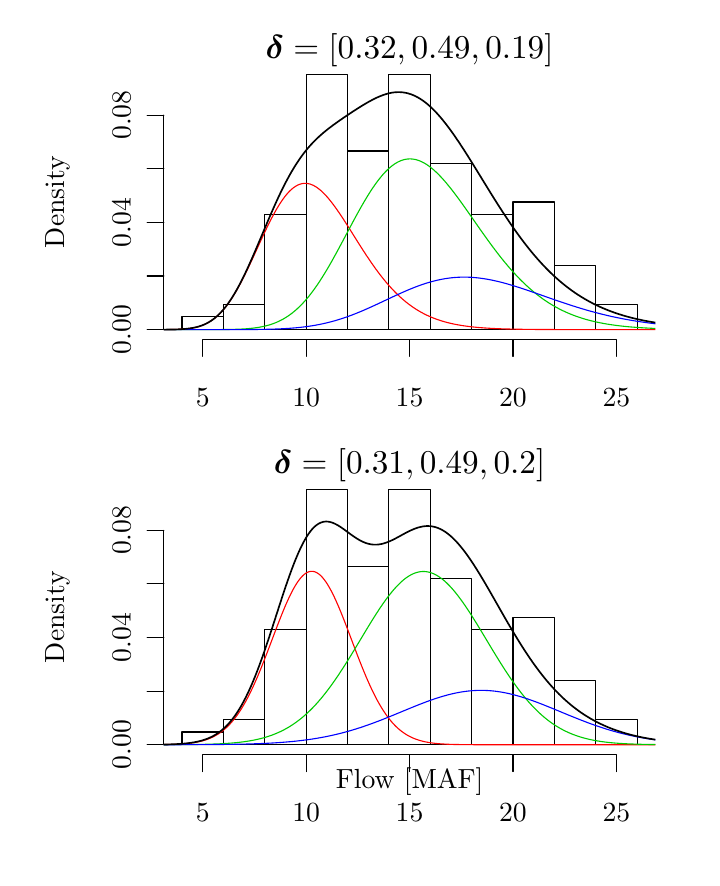
\begin{tikzpicture}[x=1pt,y=1pt]
\definecolor[named]{drawColor}{rgb}{0.00,0.00,0.00}
\definecolor[named]{fillColor}{rgb}{1.00,1.00,1.00}
\fill[color=fillColor,] (0,0) rectangle (240.00,300.00);
\begin{scope}
\path[clip] (  0.00,150.00) rectangle (240.00,300.00);
\definecolor[named]{drawColor}{rgb}{0.00,0.00,0.00}

\node[rotate= 90.00,color=drawColor,anchor=base,inner sep=0pt, outer sep=0pt, scale=  1.00] at ( 13.20,237.00) {Density%
};
\end{scope}
\begin{scope}
\path[clip] (  0.00,  0.00) rectangle (240.00,300.00);
\definecolor[named]{drawColor}{rgb}{0.00,0.00,0.00}

\draw[color=drawColor,line cap=round,line join=round,fill opacity=0.00,] ( 63.25,187.20) -- (212.75,187.20);

\draw[color=drawColor,line cap=round,line join=round,fill opacity=0.00,] ( 63.25,187.20) -- ( 63.25,181.20);

\draw[color=drawColor,line cap=round,line join=round,fill opacity=0.00,] (100.63,187.20) -- (100.63,181.20);

\draw[color=drawColor,line cap=round,line join=round,fill opacity=0.00,] (138.00,187.20) -- (138.00,181.20);

\draw[color=drawColor,line cap=round,line join=round,fill opacity=0.00,] (175.37,187.20) -- (175.37,181.20);

\draw[color=drawColor,line cap=round,line join=round,fill opacity=0.00,] (212.75,187.20) -- (212.75,181.20);

\node[color=drawColor,anchor=base,inner sep=0pt, outer sep=0pt, scale=  1.00] at ( 63.25,163.20) {5%
};

\node[color=drawColor,anchor=base,inner sep=0pt, outer sep=0pt, scale=  1.00] at (100.63,163.20) {10%
};

\node[color=drawColor,anchor=base,inner sep=0pt, outer sep=0pt, scale=  1.00] at (138.00,163.20) {15%
};

\node[color=drawColor,anchor=base,inner sep=0pt, outer sep=0pt, scale=  1.00] at (175.37,163.20) {20%
};

\node[color=drawColor,anchor=base,inner sep=0pt, outer sep=0pt, scale=  1.00] at (212.75,163.20) {25%
};

\draw[color=drawColor,line cap=round,line join=round,fill opacity=0.00,] ( 49.20,190.89) -- ( 49.20,268.36);

\draw[color=drawColor,line cap=round,line join=round,fill opacity=0.00,] ( 49.20,190.89) -- ( 43.20,190.89);

\draw[color=drawColor,line cap=round,line join=round,fill opacity=0.00,] ( 49.20,210.26) -- ( 43.20,210.26);

\draw[color=drawColor,line cap=round,line join=round,fill opacity=0.00,] ( 49.20,229.62) -- ( 43.20,229.62);

\draw[color=drawColor,line cap=round,line join=round,fill opacity=0.00,] ( 49.20,248.99) -- ( 43.20,248.99);

\draw[color=drawColor,line cap=round,line join=round,fill opacity=0.00,] ( 49.20,268.36) -- ( 43.20,268.36);

\node[rotate= 90.00,color=drawColor,anchor=base,inner sep=0pt, outer sep=0pt, scale=  1.00] at ( 37.20,190.89) {0.00%
};

\node[rotate= 90.00,color=drawColor,anchor=base,inner sep=0pt, outer sep=0pt, scale=  1.00] at ( 37.20,229.62) {0.04%
};

\node[rotate= 90.00,color=drawColor,anchor=base,inner sep=0pt, outer sep=0pt, scale=  1.00] at ( 37.20,268.36) {0.08%
};
\end{scope}
\begin{scope}
\path[clip] ( 49.20,187.20) rectangle (226.80,286.80);
\definecolor[named]{drawColor}{rgb}{0.00,0.00,0.00}

\draw[color=drawColor,line cap=round,line join=round,fill opacity=0.00,] ( 55.78,190.89) rectangle ( 70.73,195.50);

\draw[color=drawColor,line cap=round,line join=round,fill opacity=0.00,] ( 70.73,190.89) rectangle ( 85.68,200.11);

\draw[color=drawColor,line cap=round,line join=round,fill opacity=0.00,] ( 85.68,190.89) rectangle (100.63,232.39);

\draw[color=drawColor,line cap=round,line join=round,fill opacity=0.00,] (100.63,190.89) rectangle (115.58,283.11);

\draw[color=drawColor,line cap=round,line join=round,fill opacity=0.00,] (115.58,190.89) rectangle (130.53,255.44);

\draw[color=drawColor,line cap=round,line join=round,fill opacity=0.00,] (130.53,190.89) rectangle (145.47,283.11);

\draw[color=drawColor,line cap=round,line join=round,fill opacity=0.00,] (145.47,190.89) rectangle (160.42,250.83);

\draw[color=drawColor,line cap=round,line join=round,fill opacity=0.00,] (160.42,190.89) rectangle (175.37,232.39);

\draw[color=drawColor,line cap=round,line join=round,fill opacity=0.00,] (175.37,190.89) rectangle (190.32,237.00);

\draw[color=drawColor,line cap=round,line join=round,fill opacity=0.00,] (190.32,190.89) rectangle (205.27,213.94);

\draw[color=drawColor,line cap=round,line join=round,fill opacity=0.00,] (205.27,190.89) rectangle (220.22,200.11);
\definecolor[named]{drawColor}{rgb}{1.00,0.00,0.00}

\draw[color=drawColor,line cap=round,line join=round,fill opacity=0.00,] ( 29.22,190.89) --
	( 29.44,190.89) --
	( 29.67,190.89) --
	( 29.89,190.89) --
	( 30.12,190.89) --
	( 30.34,190.89) --
	( 30.57,190.89) --
	( 30.79,190.89) --
	( 31.01,190.89) --
	( 31.24,190.89) --
	( 31.46,190.89) --
	( 31.69,190.89) --
	( 31.91,190.89) --
	( 32.14,190.89) --
	( 32.36,190.89) --
	( 32.58,190.89) --
	( 32.81,190.89) --
	( 33.03,190.89) --
	( 33.26,190.89) --
	( 33.48,190.89) --
	( 33.71,190.89) --
	( 33.93,190.89) --
	( 34.15,190.89) --
	( 34.38,190.89) --
	( 34.60,190.89) --
	( 34.83,190.89) --
	( 35.05,190.89) --
	( 35.28,190.89) --
	( 35.50,190.89) --
	( 35.72,190.89) --
	( 35.95,190.89) --
	( 36.17,190.89) --
	( 36.40,190.89) --
	( 36.62,190.89) --
	( 36.85,190.89) --
	( 37.07,190.89) --
	( 37.29,190.89) --
	( 37.52,190.89) --
	( 37.74,190.89) --
	( 37.97,190.89) --
	( 38.19,190.89) --
	( 38.42,190.89) --
	( 38.64,190.89) --
	( 38.86,190.89) --
	( 39.09,190.89) --
	( 39.31,190.89) --
	( 39.54,190.89) --
	( 39.76,190.89) --
	( 39.99,190.89) --
	( 40.21,190.89) --
	( 40.43,190.89) --
	( 40.66,190.89) --
	( 40.88,190.89) --
	( 41.11,190.89) --
	( 41.33,190.89) --
	( 41.56,190.89) --
	( 41.78,190.89) --
	( 42.00,190.89) --
	( 42.23,190.89) --
	( 42.45,190.89) --
	( 42.68,190.89) --
	( 42.90,190.89) --
	( 43.13,190.89) --
	( 43.35,190.89) --
	( 43.57,190.89) --
	( 43.80,190.89) --
	( 44.02,190.89) --
	( 44.25,190.89) --
	( 44.47,190.89) --
	( 44.70,190.89) --
	( 44.92,190.89) --
	( 45.14,190.89) --
	( 45.37,190.89) --
	( 45.59,190.89) --
	( 45.82,190.89) --
	( 46.04,190.89) --
	( 46.27,190.89) --
	( 46.49,190.89) --
	( 46.71,190.89) --
	( 46.94,190.89) --
	( 47.16,190.89) --
	( 47.39,190.89) --
	( 47.61,190.89) --
	( 47.83,190.89) --
	( 48.06,190.89) --
	( 48.28,190.89) --
	( 48.51,190.90) --
	( 48.73,190.90) --
	( 48.96,190.90) --
	( 49.18,190.90) --
	( 49.40,190.90) --
	( 49.63,190.90) --
	( 49.85,190.90) --
	( 50.08,190.90) --
	( 50.30,190.91) --
	( 50.53,190.91) --
	( 50.75,190.91) --
	( 50.97,190.91) --
	( 51.20,190.91) --
	( 51.42,190.92) --
	( 51.65,190.92) --
	( 51.87,190.92) --
	( 52.10,190.93) --
	( 52.32,190.93) --
	( 52.54,190.94) --
	( 52.77,190.94) --
	( 52.99,190.95) --
	( 53.22,190.95) --
	( 53.44,190.96) --
	( 53.67,190.96) --
	( 53.89,190.97) --
	( 54.11,190.98) --
	( 54.34,190.99) --
	( 54.56,191.00) --
	( 54.79,191.01) --
	( 55.01,191.02) --
	( 55.24,191.03) --
	( 55.46,191.04) --
	( 55.68,191.06) --
	( 55.91,191.07) --
	( 56.13,191.08) --
	( 56.36,191.10) --
	( 56.58,191.12) --
	( 56.81,191.14) --
	( 57.03,191.16) --
	( 57.25,191.18) --
	( 57.48,191.20) --
	( 57.70,191.22) --
	( 57.93,191.25) --
	( 58.15,191.28) --
	( 58.38,191.31) --
	( 58.60,191.34) --
	( 58.82,191.37) --
	( 59.05,191.40) --
	( 59.27,191.44) --
	( 59.50,191.48) --
	( 59.72,191.52) --
	( 59.95,191.56) --
	( 60.17,191.60) --
	( 60.39,191.65) --
	( 60.62,191.70) --
	( 60.84,191.75) --
	( 61.07,191.81) --
	( 61.29,191.87) --
	( 61.52,191.93) --
	( 61.74,191.99) --
	( 61.96,192.06) --
	( 62.19,192.13) --
	( 62.41,192.20) --
	( 62.64,192.28) --
	( 62.86,192.36) --
	( 63.09,192.44) --
	( 63.31,192.53) --
	( 63.53,192.62) --
	( 63.76,192.72) --
	( 63.98,192.82) --
	( 64.21,192.92) --
	( 64.43,193.03) --
	( 64.66,193.14) --
	( 64.88,193.25) --
	( 65.10,193.37) --
	( 65.33,193.50) --
	( 65.55,193.63) --
	( 65.78,193.76) --
	( 66.00,193.90) --
	( 66.23,194.05) --
	( 66.45,194.20) --
	( 66.67,194.35) --
	( 66.90,194.51) --
	( 67.12,194.68) --
	( 67.35,194.85) --
	( 67.57,195.02) --
	( 67.80,195.20) --
	( 68.02,195.39) --
	( 68.24,195.58) --
	( 68.47,195.78) --
	( 68.69,195.99) --
	( 68.92,196.20) --
	( 69.14,196.41) --
	( 69.37,196.63) --
	( 69.59,196.86) --
	( 69.81,197.10) --
	( 70.04,197.34) --
	( 70.26,197.58) --
	( 70.49,197.84) --
	( 70.71,198.09) --
	( 70.94,198.36) --
	( 71.16,198.63) --
	( 71.38,198.91) --
	( 71.61,199.19) --
	( 71.83,199.48) --
	( 72.06,199.78) --
	( 72.28,200.08) --
	( 72.51,200.39) --
	( 72.73,200.70) --
	( 72.95,201.02) --
	( 73.18,201.35) --
	( 73.40,201.68) --
	( 73.63,202.02) --
	( 73.85,202.37) --
	( 74.08,202.72) --
	( 74.30,203.08) --
	( 74.52,203.44) --
	( 74.75,203.81) --
	( 74.97,204.18) --
	( 75.20,204.56) --
	( 75.42,204.95) --
	( 75.65,205.34) --
	( 75.87,205.74) --
	( 76.09,206.14) --
	( 76.32,206.55) --
	( 76.54,206.96) --
	( 76.77,207.37) --
	( 76.99,207.80) --
	( 77.22,208.22) --
	( 77.44,208.65) --
	( 77.66,209.09) --
	( 77.89,209.53) --
	( 78.11,209.97) --
	( 78.34,210.42) --
	( 78.56,210.87) --
	( 78.79,211.33) --
	( 79.01,211.79) --
	( 79.23,212.25) --
	( 79.46,212.72) --
	( 79.68,213.18) --
	( 79.91,213.66) --
	( 80.13,214.13) --
	( 80.35,214.61) --
	( 80.58,215.09) --
	( 80.80,215.57) --
	( 81.03,216.05) --
	( 81.25,216.53) --
	( 81.48,217.02) --
	( 81.70,217.51) --
	( 81.92,217.99) --
	( 82.15,218.48) --
	( 82.37,218.97) --
	( 82.60,219.46) --
	( 82.82,219.95) --
	( 83.05,220.45) --
	( 83.27,220.94) --
	( 83.49,221.43) --
	( 83.72,221.92) --
	( 83.94,222.40) --
	( 84.17,222.89) --
	( 84.39,223.38) --
	( 84.62,223.86) --
	( 84.84,224.35) --
	( 85.06,224.83) --
	( 85.29,225.31) --
	( 85.51,225.78) --
	( 85.74,226.26) --
	( 85.96,226.73) --
	( 86.19,227.20) --
	( 86.41,227.66) --
	( 86.63,228.12) --
	( 86.86,228.58) --
	( 87.08,229.04) --
	( 87.31,229.49) --
	( 87.53,229.94) --
	( 87.76,230.38) --
	( 87.98,230.81) --
	( 88.20,231.25) --
	( 88.43,231.68) --
	( 88.65,232.10) --
	( 88.88,232.52) --
	( 89.10,232.93) --
	( 89.33,233.33) --
	( 89.55,233.73) --
	( 89.77,234.13) --
	( 90.00,234.52) --
	( 90.22,234.90) --
	( 90.45,235.27) --
	( 90.67,235.64) --
	( 90.90,236.00) --
	( 91.12,236.36) --
	( 91.34,236.70) --
	( 91.57,237.04) --
	( 91.79,237.38) --
	( 92.02,237.70) --
	( 92.24,238.02) --
	( 92.47,238.33) --
	( 92.69,238.63) --
	( 92.91,238.93) --
	( 93.14,239.21) --
	( 93.36,239.49) --
	( 93.59,239.76) --
	( 93.81,240.02) --
	( 94.04,240.28) --
	( 94.26,240.52) --
	( 94.48,240.76) --
	( 94.71,240.98) --
	( 94.93,241.20) --
	( 95.16,241.41) --
	( 95.38,241.61) --
	( 95.61,241.80) --
	( 95.83,241.99) --
	( 96.05,242.16) --
	( 96.28,242.33) --
	( 96.50,242.48) --
	( 96.73,242.63) --
	( 96.95,242.77) --
	( 97.18,242.89) --
	( 97.40,243.01) --
	( 97.62,243.12) --
	( 97.85,243.23) --
	( 98.07,243.32) --
	( 98.30,243.40) --
	( 98.52,243.47) --
	( 98.75,243.54) --
	( 98.97,243.60) --
	( 99.19,243.64) --
	( 99.42,243.68) --
	( 99.64,243.71) --
	( 99.87,243.73) --
	(100.09,243.74) --
	(100.32,243.74) --
	(100.54,243.74) --
	(100.76,243.72) --
	(100.99,243.70) --
	(101.21,243.66) --
	(101.44,243.62) --
	(101.66,243.57) --
	(101.89,243.52) --
	(102.11,243.45) --
	(102.33,243.38) --
	(102.56,243.29) --
	(102.78,243.20) --
	(103.01,243.10) --
	(103.23,243.00) --
	(103.46,242.88) --
	(103.68,242.76) --
	(103.90,242.63) --
	(104.13,242.50) --
	(104.35,242.35) --
	(104.58,242.20) --
	(104.80,242.04) --
	(105.03,241.88) --
	(105.25,241.70) --
	(105.47,241.52) --
	(105.70,241.34) --
	(105.92,241.15) --
	(106.15,240.95) --
	(106.37,240.74) --
	(106.60,240.53) --
	(106.82,240.31) --
	(107.04,240.09) --
	(107.27,239.86) --
	(107.49,239.62) --
	(107.72,239.38) --
	(107.94,239.14) --
	(108.17,238.89) --
	(108.39,238.63) --
	(108.61,238.37) --
	(108.84,238.10) --
	(109.06,237.83) --
	(109.29,237.55) --
	(109.51,237.27) --
	(109.74,236.99) --
	(109.96,236.70) --
	(110.18,236.41) --
	(110.41,236.11) --
	(110.63,235.81) --
	(110.86,235.50) --
	(111.08,235.20) --
	(111.31,234.88) --
	(111.53,234.57) --
	(111.75,234.25) --
	(111.98,233.93) --
	(112.20,233.60) --
	(112.43,233.28) --
	(112.65,232.95) --
	(112.87,232.62) --
	(113.10,232.28) --
	(113.32,231.94) --
	(113.55,231.61) --
	(113.77,231.26) --
	(114.00,230.92) --
	(114.22,230.58) --
	(114.44,230.23) --
	(114.67,229.88) --
	(114.89,229.53) --
	(115.12,229.18) --
	(115.34,228.83) --
	(115.57,228.48) --
	(115.79,228.12) --
	(116.01,227.77) --
	(116.24,227.41) --
	(116.46,227.06) --
	(116.69,226.70) --
	(116.91,226.34) --
	(117.14,225.99) --
	(117.36,225.63) --
	(117.58,225.27) --
	(117.81,224.91) --
	(118.03,224.55) --
	(118.26,224.20) --
	(118.48,223.84) --
	(118.71,223.48) --
	(118.93,223.13) --
	(119.15,222.77) --
	(119.38,222.41) --
	(119.60,222.06) --
	(119.83,221.70) --
	(120.05,221.35) --
	(120.28,221.00) --
	(120.50,220.65) --
	(120.72,220.30) --
	(120.95,219.95) --
	(121.17,219.60) --
	(121.40,219.25) --
	(121.62,218.91) --
	(121.85,218.57) --
	(122.07,218.22) --
	(122.29,217.88) --
	(122.52,217.54) --
	(122.74,217.21) --
	(122.97,216.87) --
	(123.19,216.54) --
	(123.42,216.20) --
	(123.64,215.87) --
	(123.86,215.55) --
	(124.09,215.22) --
	(124.31,214.89) --
	(124.54,214.57) --
	(124.76,214.25) --
	(124.99,213.93) --
	(125.21,213.62) --
	(125.43,213.31) --
	(125.66,212.99) --
	(125.88,212.68) --
	(126.11,212.38) --
	(126.33,212.07) --
	(126.56,211.77) --
	(126.78,211.47) --
	(127.00,211.18) --
	(127.23,210.88) --
	(127.45,210.59) --
	(127.68,210.30) --
	(127.90,210.01) --
	(128.13,209.73) --
	(128.35,209.45) --
	(128.57,209.17) --
	(128.80,208.89) --
	(129.02,208.62) --
	(129.25,208.35) --
	(129.47,208.08) --
	(129.70,207.81) --
	(129.92,207.55) --
	(130.14,207.29) --
	(130.37,207.03) --
	(130.59,206.78) --
	(130.82,206.52) --
	(131.04,206.28) --
	(131.27,206.03) --
	(131.49,205.78) --
	(131.71,205.54) --
	(131.94,205.30) --
	(132.16,205.07) --
	(132.39,204.84) --
	(132.61,204.60) --
	(132.84,204.38) --
	(133.06,204.15) --
	(133.28,203.93) --
	(133.51,203.71) --
	(133.73,203.49) --
	(133.96,203.28) --
	(134.18,203.07) --
	(134.41,202.86) --
	(134.63,202.65) --
	(134.85,202.45) --
	(135.08,202.25) --
	(135.30,202.05) --
	(135.53,201.85) --
	(135.75,201.66) --
	(135.98,201.47) --
	(136.20,201.28) --
	(136.42,201.10) --
	(136.65,200.91) --
	(136.87,200.73) --
	(137.10,200.56) --
	(137.32,200.38) --
	(137.55,200.21) --
	(137.77,200.04) --
	(137.99,199.87) --
	(138.22,199.71) --
	(138.44,199.54) --
	(138.67,199.38) --
	(138.89,199.22) --
	(139.12,199.07) --
	(139.34,198.91) --
	(139.56,198.76) --
	(139.79,198.61) --
	(140.01,198.47) --
	(140.24,198.32) --
	(140.46,198.18) --
	(140.69,198.04) --
	(140.91,197.90) --
	(141.13,197.77) --
	(141.36,197.63) --
	(141.58,197.50) --
	(141.81,197.37) --
	(142.03,197.25) --
	(142.26,197.12) --
	(142.48,197.00) --
	(142.70,196.88) --
	(142.93,196.76) --
	(143.15,196.64) --
	(143.38,196.53) --
	(143.60,196.41) --
	(143.83,196.30) --
	(144.05,196.19) --
	(144.27,196.09) --
	(144.50,195.98) --
	(144.72,195.88) --
	(144.95,195.78) --
	(145.17,195.68) --
	(145.40,195.58) --
	(145.62,195.48) --
	(145.84,195.39) --
	(146.07,195.29) --
	(146.29,195.20) --
	(146.52,195.11) --
	(146.74,195.02) --
	(146.96,194.93) --
	(147.19,194.85) --
	(147.41,194.77) --
	(147.64,194.68) --
	(147.86,194.60) --
	(148.09,194.52) --
	(148.31,194.45) --
	(148.53,194.37) --
	(148.76,194.30) --
	(148.98,194.22) --
	(149.21,194.15) --
	(149.43,194.08) --
	(149.66,194.01) --
	(149.88,193.94) --
	(150.10,193.88) --
	(150.33,193.81) --
	(150.55,193.75) --
	(150.78,193.68) --
	(151.00,193.62) --
	(151.23,193.56) --
	(151.45,193.50) --
	(151.67,193.44) --
	(151.90,193.39) --
	(152.12,193.33) --
	(152.35,193.28) --
	(152.57,193.22) --
	(152.80,193.17) --
	(153.02,193.12) --
	(153.24,193.07) --
	(153.47,193.02) --
	(153.69,192.97) --
	(153.92,192.92) --
	(154.14,192.88) --
	(154.37,192.83) --
	(154.59,192.79) --
	(154.81,192.74) --
	(155.04,192.70) --
	(155.26,192.66) --
	(155.49,192.62) --
	(155.71,192.58) --
	(155.94,192.54) --
	(156.16,192.50) --
	(156.38,192.46) --
	(156.61,192.42) --
	(156.83,192.39) --
	(157.06,192.35) --
	(157.28,192.32) --
	(157.51,192.28) --
	(157.73,192.25) --
	(157.95,192.22) --
	(158.18,192.19) --
	(158.40,192.16) --
	(158.63,192.13) --
	(158.85,192.10) --
	(159.08,192.07) --
	(159.30,192.04) --
	(159.52,192.01) --
	(159.75,191.98) --
	(159.97,191.96) --
	(160.20,191.93) --
	(160.42,191.91) --
	(160.65,191.88) --
	(160.87,191.86) --
	(161.09,191.83) --
	(161.32,191.81) --
	(161.54,191.79) --
	(161.77,191.77) --
	(161.99,191.74) --
	(162.22,191.72) --
	(162.44,191.70) --
	(162.66,191.68) --
	(162.89,191.66) --
	(163.11,191.64) --
	(163.34,191.62) --
	(163.56,191.61) --
	(163.79,191.59) --
	(164.01,191.57) --
	(164.23,191.55) --
	(164.46,191.54) --
	(164.68,191.52) --
	(164.91,191.50) --
	(165.13,191.49) --
	(165.36,191.47) --
	(165.58,191.46) --
	(165.80,191.44) --
	(166.03,191.43) --
	(166.25,191.42) --
	(166.48,191.40) --
	(166.70,191.39) --
	(166.93,191.38) --
	(167.15,191.36) --
	(167.37,191.35) --
	(167.60,191.34) --
	(167.82,191.33) --
	(168.05,191.32) --
	(168.27,191.31) --
	(168.50,191.29) --
	(168.72,191.28) --
	(168.94,191.27) --
	(169.17,191.26) --
	(169.39,191.25) --
	(169.62,191.24) --
	(169.84,191.24) --
	(170.07,191.23) --
	(170.29,191.22) --
	(170.51,191.21) --
	(170.74,191.20) --
	(170.96,191.19) --
	(171.19,191.18) --
	(171.41,191.18) --
	(171.64,191.17) --
	(171.86,191.16) --
	(172.08,191.15) --
	(172.31,191.15) --
	(172.53,191.14) --
	(172.76,191.13) --
	(172.98,191.13) --
	(173.21,191.12) --
	(173.43,191.11) --
	(173.65,191.11) --
	(173.88,191.10) --
	(174.10,191.10) --
	(174.33,191.09) --
	(174.55,191.08) --
	(174.78,191.08) --
	(175.00,191.07) --
	(175.22,191.07) --
	(175.45,191.06) --
	(175.67,191.06) --
	(175.90,191.05) --
	(176.12,191.05) --
	(176.35,191.05) --
	(176.57,191.04) --
	(176.79,191.04) --
	(177.02,191.03) --
	(177.24,191.03) --
	(177.47,191.03) --
	(177.69,191.02) --
	(177.92,191.02) --
	(178.14,191.01) --
	(178.36,191.01) --
	(178.59,191.01) --
	(178.81,191.00) --
	(179.04,191.00) --
	(179.26,191.00) --
	(179.48,190.99) --
	(179.71,190.99) --
	(179.93,190.99) --
	(180.16,190.99) --
	(180.38,190.98) --
	(180.61,190.98) --
	(180.83,190.98) --
	(181.05,190.98) --
	(181.28,190.97) --
	(181.50,190.97) --
	(181.73,190.97) --
	(181.95,190.97) --
	(182.18,190.96) --
	(182.40,190.96) --
	(182.62,190.96) --
	(182.85,190.96) --
	(183.07,190.96) --
	(183.30,190.95) --
	(183.52,190.95) --
	(183.75,190.95) --
	(183.97,190.95) --
	(184.19,190.95) --
	(184.42,190.95) --
	(184.64,190.94) --
	(184.87,190.94) --
	(185.09,190.94) --
	(185.32,190.94) --
	(185.54,190.94) --
	(185.76,190.94) --
	(185.99,190.93) --
	(186.21,190.93) --
	(186.44,190.93) --
	(186.66,190.93) --
	(186.89,190.93) --
	(187.11,190.93) --
	(187.33,190.93) --
	(187.56,190.93) --
	(187.78,190.92) --
	(188.01,190.92) --
	(188.23,190.92) --
	(188.46,190.92) --
	(188.68,190.92) --
	(188.90,190.92) --
	(189.13,190.92) --
	(189.35,190.92) --
	(189.58,190.92) --
	(189.80,190.92) --
	(190.03,190.92) --
	(190.25,190.91) --
	(190.47,190.91) --
	(190.70,190.91) --
	(190.92,190.91) --
	(191.15,190.91) --
	(191.37,190.91) --
	(191.60,190.91) --
	(191.82,190.91) --
	(192.04,190.91) --
	(192.27,190.91) --
	(192.49,190.91) --
	(192.72,190.91) --
	(192.94,190.91) --
	(193.17,190.91) --
	(193.39,190.91) --
	(193.61,190.91) --
	(193.84,190.90) --
	(194.06,190.90) --
	(194.29,190.90) --
	(194.51,190.90) --
	(194.74,190.90) --
	(194.96,190.90) --
	(195.18,190.90) --
	(195.41,190.90) --
	(195.63,190.90) --
	(195.86,190.90) --
	(196.08,190.90) --
	(196.31,190.90) --
	(196.53,190.90) --
	(196.75,190.90) --
	(196.98,190.90) --
	(197.20,190.90) --
	(197.43,190.90) --
	(197.65,190.90) --
	(197.88,190.90) --
	(198.10,190.90) --
	(198.32,190.90) --
	(198.55,190.90) --
	(198.77,190.90) --
	(199.00,190.90) --
	(199.22,190.90) --
	(199.45,190.90) --
	(199.67,190.90) --
	(199.89,190.90) --
	(200.12,190.90) --
	(200.34,190.90) --
	(200.57,190.90) --
	(200.79,190.89) --
	(201.02,190.89) --
	(201.24,190.89) --
	(201.46,190.89) --
	(201.69,190.89) --
	(201.91,190.89) --
	(202.14,190.89) --
	(202.36,190.89) --
	(202.59,190.89) --
	(202.81,190.89) --
	(203.03,190.89) --
	(203.26,190.89) --
	(203.48,190.89) --
	(203.71,190.89) --
	(203.93,190.89) --
	(204.16,190.89) --
	(204.38,190.89) --
	(204.60,190.89) --
	(204.83,190.89) --
	(205.05,190.89) --
	(205.28,190.89) --
	(205.50,190.89) --
	(205.73,190.89) --
	(205.95,190.89) --
	(206.17,190.89) --
	(206.40,190.89) --
	(206.62,190.89) --
	(206.85,190.89) --
	(207.07,190.89) --
	(207.30,190.89) --
	(207.52,190.89) --
	(207.74,190.89) --
	(207.97,190.89) --
	(208.19,190.89) --
	(208.42,190.89) --
	(208.64,190.89) --
	(208.87,190.89) --
	(209.09,190.89) --
	(209.31,190.89) --
	(209.54,190.89) --
	(209.76,190.89) --
	(209.99,190.89) --
	(210.21,190.89) --
	(210.44,190.89) --
	(210.66,190.89) --
	(210.88,190.89) --
	(211.11,190.89) --
	(211.33,190.89) --
	(211.56,190.89) --
	(211.78,190.89) --
	(212.00,190.89) --
	(212.23,190.89) --
	(212.45,190.89) --
	(212.68,190.89) --
	(212.90,190.89) --
	(213.13,190.89) --
	(213.35,190.89) --
	(213.57,190.89) --
	(213.80,190.89) --
	(214.02,190.89) --
	(214.25,190.89) --
	(214.47,190.89) --
	(214.70,190.89) --
	(214.92,190.89) --
	(215.14,190.89) --
	(215.37,190.89) --
	(215.59,190.89) --
	(215.82,190.89) --
	(216.04,190.89) --
	(216.27,190.89) --
	(216.49,190.89) --
	(216.71,190.89) --
	(216.94,190.89) --
	(217.16,190.89) --
	(217.39,190.89) --
	(217.61,190.89) --
	(217.84,190.89) --
	(218.06,190.89) --
	(218.28,190.89) --
	(218.51,190.89) --
	(218.73,190.89) --
	(218.96,190.89) --
	(219.18,190.89) --
	(219.41,190.89) --
	(219.63,190.89) --
	(219.85,190.89) --
	(220.08,190.89) --
	(220.30,190.89) --
	(220.53,190.89) --
	(220.75,190.89) --
	(220.98,190.89) --
	(221.20,190.89) --
	(221.42,190.89) --
	(221.65,190.89) --
	(221.87,190.89) --
	(222.10,190.89) --
	(222.32,190.89) --
	(222.55,190.89) --
	(222.77,190.89) --
	(222.99,190.89) --
	(223.22,190.89) --
	(223.44,190.89) --
	(223.67,190.89) --
	(223.89,190.89) --
	(224.12,190.89) --
	(224.34,190.89) --
	(224.56,190.89) --
	(224.79,190.89) --
	(225.01,190.89) --
	(225.24,190.89) --
	(225.46,190.89) --
	(225.69,190.89) --
	(225.91,190.89) --
	(226.13,190.89) --
	(226.36,190.89) --
	(226.58,190.89) --
	(226.81,190.89) --
	(227.03,190.89) --
	(227.26,190.89) --
	(227.48,190.89) --
	(227.70,190.89) --
	(227.93,190.89) --
	(228.15,190.89) --
	(228.38,190.89) --
	(228.60,190.89) --
	(228.83,190.89) --
	(229.05,190.89) --
	(229.27,190.89) --
	(229.50,190.89) --
	(229.72,190.89) --
	(229.95,190.89) --
	(230.17,190.89) --
	(230.40,190.89) --
	(230.62,190.89) --
	(230.84,190.89) --
	(231.07,190.89) --
	(231.29,190.89) --
	(231.52,190.89) --
	(231.74,190.89) --
	(231.97,190.89) --
	(232.19,190.89) --
	(232.41,190.89) --
	(232.64,190.89) --
	(232.86,190.89) --
	(233.09,190.89) --
	(233.31,190.89) --
	(233.54,190.89) --
	(233.76,190.89) --
	(233.98,190.89) --
	(234.21,190.89) --
	(234.43,190.89) --
	(234.66,190.89) --
	(234.88,190.89) --
	(235.11,190.89) --
	(235.33,190.89) --
	(235.55,190.89) --
	(235.78,190.89) --
	(236.00,190.89) --
	(236.23,190.89) --
	(236.45,190.89) --
	(236.68,190.89) --
	(236.90,190.89) --
	(237.12,190.89) --
	(237.35,190.89) --
	(237.57,190.89) --
	(237.80,190.89) --
	(238.02,190.89) --
	(238.25,190.89) --
	(238.47,190.89) --
	(238.69,190.89) --
	(238.92,190.89) --
	(239.14,190.89) --
	(239.37,190.89) --
	(239.59,190.89) --
	(239.82,190.89) --
	(240.00,190.89);
\definecolor[named]{drawColor}{rgb}{0.00,0.80,0.00}

\draw[color=drawColor,line cap=round,line join=round,fill opacity=0.00,] ( 29.22,190.89) --
	( 29.44,190.89) --
	( 29.67,190.89) --
	( 29.89,190.89) --
	( 30.12,190.89) --
	( 30.34,190.89) --
	( 30.57,190.89) --
	( 30.79,190.89) --
	( 31.01,190.89) --
	( 31.24,190.89) --
	( 31.46,190.89) --
	( 31.69,190.89) --
	( 31.91,190.89) --
	( 32.14,190.89) --
	( 32.36,190.89) --
	( 32.58,190.89) --
	( 32.81,190.89) --
	( 33.03,190.89) --
	( 33.26,190.89) --
	( 33.48,190.89) --
	( 33.71,190.89) --
	( 33.93,190.89) --
	( 34.15,190.89) --
	( 34.38,190.89) --
	( 34.60,190.89) --
	( 34.83,190.89) --
	( 35.05,190.89) --
	( 35.28,190.89) --
	( 35.50,190.89) --
	( 35.72,190.89) --
	( 35.95,190.89) --
	( 36.17,190.89) --
	( 36.40,190.89) --
	( 36.62,190.89) --
	( 36.85,190.89) --
	( 37.07,190.89) --
	( 37.29,190.89) --
	( 37.52,190.89) --
	( 37.74,190.89) --
	( 37.97,190.89) --
	( 38.19,190.89) --
	( 38.42,190.89) --
	( 38.64,190.89) --
	( 38.86,190.89) --
	( 39.09,190.89) --
	( 39.31,190.89) --
	( 39.54,190.89) --
	( 39.76,190.89) --
	( 39.99,190.89) --
	( 40.21,190.89) --
	( 40.43,190.89) --
	( 40.66,190.89) --
	( 40.88,190.89) --
	( 41.11,190.89) --
	( 41.33,190.89) --
	( 41.56,190.89) --
	( 41.78,190.89) --
	( 42.00,190.89) --
	( 42.23,190.89) --
	( 42.45,190.89) --
	( 42.68,190.89) --
	( 42.90,190.89) --
	( 43.13,190.89) --
	( 43.35,190.89) --
	( 43.57,190.89) --
	( 43.80,190.89) --
	( 44.02,190.89) --
	( 44.25,190.89) --
	( 44.47,190.89) --
	( 44.70,190.89) --
	( 44.92,190.89) --
	( 45.14,190.89) --
	( 45.37,190.89) --
	( 45.59,190.89) --
	( 45.82,190.89) --
	( 46.04,190.89) --
	( 46.27,190.89) --
	( 46.49,190.89) --
	( 46.71,190.89) --
	( 46.94,190.89) --
	( 47.16,190.89) --
	( 47.39,190.89) --
	( 47.61,190.89) --
	( 47.83,190.89) --
	( 48.06,190.89) --
	( 48.28,190.89) --
	( 48.51,190.89) --
	( 48.73,190.89) --
	( 48.96,190.89) --
	( 49.18,190.89) --
	( 49.40,190.89) --
	( 49.63,190.89) --
	( 49.85,190.89) --
	( 50.08,190.89) --
	( 50.30,190.89) --
	( 50.53,190.89) --
	( 50.75,190.89) --
	( 50.97,190.89) --
	( 51.20,190.89) --
	( 51.42,190.89) --
	( 51.65,190.89) --
	( 51.87,190.89) --
	( 52.10,190.89) --
	( 52.32,190.89) --
	( 52.54,190.89) --
	( 52.77,190.89) --
	( 52.99,190.89) --
	( 53.22,190.89) --
	( 53.44,190.89) --
	( 53.67,190.89) --
	( 53.89,190.89) --
	( 54.11,190.89) --
	( 54.34,190.89) --
	( 54.56,190.89) --
	( 54.79,190.89) --
	( 55.01,190.89) --
	( 55.24,190.89) --
	( 55.46,190.89) --
	( 55.68,190.89) --
	( 55.91,190.89) --
	( 56.13,190.89) --
	( 56.36,190.89) --
	( 56.58,190.89) --
	( 56.81,190.89) --
	( 57.03,190.89) --
	( 57.25,190.89) --
	( 57.48,190.89) --
	( 57.70,190.89) --
	( 57.93,190.89) --
	( 58.15,190.89) --
	( 58.38,190.89) --
	( 58.60,190.89) --
	( 58.82,190.89) --
	( 59.05,190.89) --
	( 59.27,190.89) --
	( 59.50,190.89) --
	( 59.72,190.89) --
	( 59.95,190.89) --
	( 60.17,190.89) --
	( 60.39,190.89) --
	( 60.62,190.89) --
	( 60.84,190.89) --
	( 61.07,190.89) --
	( 61.29,190.89) --
	( 61.52,190.89) --
	( 61.74,190.89) --
	( 61.96,190.89) --
	( 62.19,190.89) --
	( 62.41,190.89) --
	( 62.64,190.89) --
	( 62.86,190.89) --
	( 63.09,190.89) --
	( 63.31,190.89) --
	( 63.53,190.89) --
	( 63.76,190.89) --
	( 63.98,190.89) --
	( 64.21,190.89) --
	( 64.43,190.89) --
	( 64.66,190.89) --
	( 64.88,190.89) --
	( 65.10,190.89) --
	( 65.33,190.89) --
	( 65.55,190.89) --
	( 65.78,190.89) --
	( 66.00,190.89) --
	( 66.23,190.90) --
	( 66.45,190.90) --
	( 66.67,190.90) --
	( 66.90,190.90) --
	( 67.12,190.90) --
	( 67.35,190.90) --
	( 67.57,190.90) --
	( 67.80,190.90) --
	( 68.02,190.90) --
	( 68.24,190.90) --
	( 68.47,190.90) --
	( 68.69,190.90) --
	( 68.92,190.91) --
	( 69.14,190.91) --
	( 69.37,190.91) --
	( 69.59,190.91) --
	( 69.81,190.91) --
	( 70.04,190.91) --
	( 70.26,190.92) --
	( 70.49,190.92) --
	( 70.71,190.92) --
	( 70.94,190.92) --
	( 71.16,190.92) --
	( 71.38,190.93) --
	( 71.61,190.93) --
	( 71.83,190.93) --
	( 72.06,190.94) --
	( 72.28,190.94) --
	( 72.51,190.94) --
	( 72.73,190.95) --
	( 72.95,190.95) --
	( 73.18,190.96) --
	( 73.40,190.96) --
	( 73.63,190.96) --
	( 73.85,190.97) --
	( 74.08,190.97) --
	( 74.30,190.98) --
	( 74.52,190.99) --
	( 74.75,190.99) --
	( 74.97,191.00) --
	( 75.20,191.01) --
	( 75.42,191.01) --
	( 75.65,191.02) --
	( 75.87,191.03) --
	( 76.09,191.04) --
	( 76.32,191.05) --
	( 76.54,191.06) --
	( 76.77,191.07) --
	( 76.99,191.08) --
	( 77.22,191.09) --
	( 77.44,191.10) --
	( 77.66,191.11) --
	( 77.89,191.12) --
	( 78.11,191.14) --
	( 78.34,191.15) --
	( 78.56,191.17) --
	( 78.79,191.18) --
	( 79.01,191.20) --
	( 79.23,191.22) --
	( 79.46,191.23) --
	( 79.68,191.25) --
	( 79.91,191.27) --
	( 80.13,191.29) --
	( 80.35,191.31) --
	( 80.58,191.33) --
	( 80.80,191.36) --
	( 81.03,191.38) --
	( 81.25,191.40) --
	( 81.48,191.43) --
	( 81.70,191.46) --
	( 81.92,191.49) --
	( 82.15,191.52) --
	( 82.37,191.55) --
	( 82.60,191.58) --
	( 82.82,191.61) --
	( 83.05,191.64) --
	( 83.27,191.68) --
	( 83.49,191.72) --
	( 83.72,191.75) --
	( 83.94,191.79) --
	( 84.17,191.84) --
	( 84.39,191.88) --
	( 84.62,191.92) --
	( 84.84,191.97) --
	( 85.06,192.02) --
	( 85.29,192.06) --
	( 85.51,192.12) --
	( 85.74,192.17) --
	( 85.96,192.22) --
	( 86.19,192.28) --
	( 86.41,192.34) --
	( 86.63,192.40) --
	( 86.86,192.46) --
	( 87.08,192.52) --
	( 87.31,192.59) --
	( 87.53,192.66) --
	( 87.76,192.73) --
	( 87.98,192.80) --
	( 88.20,192.88) --
	( 88.43,192.95) --
	( 88.65,193.03) --
	( 88.88,193.11) --
	( 89.10,193.20) --
	( 89.33,193.29) --
	( 89.55,193.37) --
	( 89.77,193.47) --
	( 90.00,193.56) --
	( 90.22,193.66) --
	( 90.45,193.76) --
	( 90.67,193.86) --
	( 90.90,193.97) --
	( 91.12,194.07) --
	( 91.34,194.19) --
	( 91.57,194.30) --
	( 91.79,194.42) --
	( 92.02,194.54) --
	( 92.24,194.66) --
	( 92.47,194.79) --
	( 92.69,194.92) --
	( 92.91,195.05) --
	( 93.14,195.18) --
	( 93.36,195.32) --
	( 93.59,195.47) --
	( 93.81,195.61) --
	( 94.04,195.76) --
	( 94.26,195.91) --
	( 94.48,196.07) --
	( 94.71,196.23) --
	( 94.93,196.39) --
	( 95.16,196.56) --
	( 95.38,196.73) --
	( 95.61,196.90) --
	( 95.83,197.08) --
	( 96.05,197.26) --
	( 96.28,197.44) --
	( 96.50,197.63) --
	( 96.73,197.82) --
	( 96.95,198.02) --
	( 97.18,198.22) --
	( 97.40,198.42) --
	( 97.62,198.63) --
	( 97.85,198.84) --
	( 98.07,199.05) --
	( 98.30,199.27) --
	( 98.52,199.49) --
	( 98.75,199.72) --
	( 98.97,199.95) --
	( 99.19,200.18) --
	( 99.42,200.42) --
	( 99.64,200.66) --
	( 99.87,200.91) --
	(100.09,201.16) --
	(100.32,201.41) --
	(100.54,201.67) --
	(100.76,201.93) --
	(100.99,202.20) --
	(101.21,202.46) --
	(101.44,202.74) --
	(101.66,203.01) --
	(101.89,203.30) --
	(102.11,203.58) --
	(102.33,203.87) --
	(102.56,204.16) --
	(102.78,204.46) --
	(103.01,204.76) --
	(103.23,205.06) --
	(103.46,205.37) --
	(103.68,205.68) --
	(103.90,205.99) --
	(104.13,206.31) --
	(104.35,206.64) --
	(104.58,206.96) --
	(104.80,207.29) --
	(105.03,207.62) --
	(105.25,207.96) --
	(105.47,208.30) --
	(105.70,208.64) --
	(105.92,208.99) --
	(106.15,209.34) --
	(106.37,209.69) --
	(106.60,210.05) --
	(106.82,210.41) --
	(107.04,210.77) --
	(107.27,211.14) --
	(107.49,211.50) --
	(107.72,211.88) --
	(107.94,212.25) --
	(108.17,212.63) --
	(108.39,213.01) --
	(108.61,213.39) --
	(108.84,213.77) --
	(109.06,214.16) --
	(109.29,214.55) --
	(109.51,214.94) --
	(109.74,215.34) --
	(109.96,215.73) --
	(110.18,216.13) --
	(110.41,216.53) --
	(110.63,216.94) --
	(110.86,217.34) --
	(111.08,217.75) --
	(111.31,218.16) --
	(111.53,218.57) --
	(111.75,218.98) --
	(111.98,219.39) --
	(112.20,219.81) --
	(112.43,220.22) --
	(112.65,220.64) --
	(112.87,221.06) --
	(113.10,221.48) --
	(113.32,221.90) --
	(113.55,222.32) --
	(113.77,222.74) --
	(114.00,223.16) --
	(114.22,223.59) --
	(114.44,224.01) --
	(114.67,224.43) --
	(114.89,224.86) --
	(115.12,225.28) --
	(115.34,225.70) --
	(115.57,226.13) --
	(115.79,226.55) --
	(116.01,226.97) --
	(116.24,227.40) --
	(116.46,227.82) --
	(116.69,228.24) --
	(116.91,228.66) --
	(117.14,229.08) --
	(117.36,229.50) --
	(117.58,229.92) --
	(117.81,230.34) --
	(118.03,230.76) --
	(118.26,231.17) --
	(118.48,231.58) --
	(118.71,232.00) --
	(118.93,232.41) --
	(119.15,232.82) --
	(119.38,233.22) --
	(119.60,233.63) --
	(119.83,234.03) --
	(120.05,234.43) --
	(120.28,234.83) --
	(120.50,235.22) --
	(120.72,235.62) --
	(120.95,236.01) --
	(121.17,236.40) --
	(121.40,236.78) --
	(121.62,237.17) --
	(121.85,237.55) --
	(122.07,237.92) --
	(122.29,238.30) --
	(122.52,238.67) --
	(122.74,239.04) --
	(122.97,239.40) --
	(123.19,239.76) --
	(123.42,240.12) --
	(123.64,240.47) --
	(123.86,240.82) --
	(124.09,241.16) --
	(124.31,241.51) --
	(124.54,241.84) --
	(124.76,242.18) --
	(124.99,242.51) --
	(125.21,242.83) --
	(125.43,243.15) --
	(125.66,243.47) --
	(125.88,243.78) --
	(126.11,244.09) --
	(126.33,244.39) --
	(126.56,244.69) --
	(126.78,244.98) --
	(127.00,245.27) --
	(127.23,245.55) --
	(127.45,245.83) --
	(127.68,246.11) --
	(127.90,246.38) --
	(128.13,246.64) --
	(128.35,246.90) --
	(128.57,247.15) --
	(128.80,247.40) --
	(129.02,247.64) --
	(129.25,247.88) --
	(129.47,248.11) --
	(129.70,248.33) --
	(129.92,248.55) --
	(130.14,248.77) --
	(130.37,248.98) --
	(130.59,249.18) --
	(130.82,249.38) --
	(131.04,249.57) --
	(131.27,249.76) --
	(131.49,249.94) --
	(131.71,250.11) --
	(131.94,250.28) --
	(132.16,250.44) --
	(132.39,250.60) --
	(132.61,250.75) --
	(132.84,250.90) --
	(133.06,251.04) --
	(133.28,251.17) --
	(133.51,251.30) --
	(133.73,251.42) --
	(133.96,251.53) --
	(134.18,251.64) --
	(134.41,251.74) --
	(134.63,251.84) --
	(134.85,251.93) --
	(135.08,252.02) --
	(135.30,252.10) --
	(135.53,252.17) --
	(135.75,252.23) --
	(135.98,252.30) --
	(136.20,252.35) --
	(136.42,252.40) --
	(136.65,252.44) --
	(136.87,252.48) --
	(137.10,252.51) --
	(137.32,252.53) --
	(137.55,252.55) --
	(137.77,252.56) --
	(137.99,252.57) --
	(138.22,252.57) --
	(138.44,252.57) --
	(138.67,252.55) --
	(138.89,252.54) --
	(139.12,252.51) --
	(139.34,252.49) --
	(139.56,252.45) --
	(139.79,252.41) --
	(140.01,252.37) --
	(140.24,252.32) --
	(140.46,252.26) --
	(140.69,252.20) --
	(140.91,252.13) --
	(141.13,252.05) --
	(141.36,251.98) --
	(141.58,251.89) --
	(141.81,251.80) --
	(142.03,251.71) --
	(142.26,251.61) --
	(142.48,251.50) --
	(142.70,251.39) --
	(142.93,251.28) --
	(143.15,251.15) --
	(143.38,251.03) --
	(143.60,250.90) --
	(143.83,250.76) --
	(144.05,250.62) --
	(144.27,250.48) --
	(144.50,250.33) --
	(144.72,250.17) --
	(144.95,250.01) --
	(145.17,249.85) --
	(145.40,249.68) --
	(145.62,249.51) --
	(145.84,249.33) --
	(146.07,249.15) --
	(146.29,248.96) --
	(146.52,248.77) --
	(146.74,248.58) --
	(146.96,248.38) --
	(147.19,248.18) --
	(147.41,247.97) --
	(147.64,247.76) --
	(147.86,247.55) --
	(148.09,247.33) --
	(148.31,247.11) --
	(148.53,246.88) --
	(148.76,246.65) --
	(148.98,246.42) --
	(149.21,246.18) --
	(149.43,245.95) --
	(149.66,245.70) --
	(149.88,245.46) --
	(150.10,245.21) --
	(150.33,244.96) --
	(150.55,244.70) --
	(150.78,244.44) --
	(151.00,244.18) --
	(151.23,243.92) --
	(151.45,243.65) --
	(151.67,243.39) --
	(151.90,243.11) --
	(152.12,242.84) --
	(152.35,242.56) --
	(152.57,242.29) --
	(152.80,242.00) --
	(153.02,241.72) --
	(153.24,241.44) --
	(153.47,241.15) --
	(153.69,240.86) --
	(153.92,240.57) --
	(154.14,240.27) --
	(154.37,239.98) --
	(154.59,239.68) --
	(154.81,239.38) --
	(155.04,239.08) --
	(155.26,238.78) --
	(155.49,238.47) --
	(155.71,238.17) --
	(155.94,237.86) --
	(156.16,237.55) --
	(156.38,237.24) --
	(156.61,236.93) --
	(156.83,236.62) --
	(157.06,236.31) --
	(157.28,236.00) --
	(157.51,235.68) --
	(157.73,235.37) --
	(157.95,235.05) --
	(158.18,234.73) --
	(158.40,234.41) --
	(158.63,234.10) --
	(158.85,233.78) --
	(159.08,233.46) --
	(159.30,233.14) --
	(159.52,232.82) --
	(159.75,232.50) --
	(159.97,232.17) --
	(160.20,231.85) --
	(160.42,231.53) --
	(160.65,231.21) --
	(160.87,230.89) --
	(161.09,230.57) --
	(161.32,230.24) --
	(161.54,229.92) --
	(161.77,229.60) --
	(161.99,229.28) --
	(162.22,228.96) --
	(162.44,228.63) --
	(162.66,228.31) --
	(162.89,227.99) --
	(163.11,227.67) --
	(163.34,227.35) --
	(163.56,227.03) --
	(163.79,226.71) --
	(164.01,226.40) --
	(164.23,226.08) --
	(164.46,225.76) --
	(164.68,225.45) --
	(164.91,225.13) --
	(165.13,224.82) --
	(165.36,224.50) --
	(165.58,224.19) --
	(165.80,223.88) --
	(166.03,223.56) --
	(166.25,223.25) --
	(166.48,222.94) --
	(166.70,222.64) --
	(166.93,222.33) --
	(167.15,222.02) --
	(167.37,221.72) --
	(167.60,221.41) --
	(167.82,221.11) --
	(168.05,220.81) --
	(168.27,220.51) --
	(168.50,220.21) --
	(168.72,219.91) --
	(168.94,219.62) --
	(169.17,219.32) --
	(169.39,219.03) --
	(169.62,218.74) --
	(169.84,218.44) --
	(170.07,218.16) --
	(170.29,217.87) --
	(170.51,217.58) --
	(170.74,217.30) --
	(170.96,217.01) --
	(171.19,216.73) --
	(171.41,216.45) --
	(171.64,216.17) --
	(171.86,215.90) --
	(172.08,215.62) --
	(172.31,215.35) --
	(172.53,215.07) --
	(172.76,214.80) --
	(172.98,214.54) --
	(173.21,214.27) --
	(173.43,214.00) --
	(173.65,213.74) --
	(173.88,213.48) --
	(174.10,213.22) --
	(174.33,212.96) --
	(174.55,212.70) --
	(174.78,212.45) --
	(175.00,212.20) --
	(175.22,211.95) --
	(175.45,211.70) --
	(175.67,211.45) --
	(175.90,211.20) --
	(176.12,210.96) --
	(176.35,210.72) --
	(176.57,210.48) --
	(176.79,210.24) --
	(177.02,210.01) --
	(177.24,209.77) --
	(177.47,209.54) --
	(177.69,209.31) --
	(177.92,209.08) --
	(178.14,208.85) --
	(178.36,208.63) --
	(178.59,208.41) --
	(178.81,208.19) --
	(179.04,207.97) --
	(179.26,207.75) --
	(179.48,207.53) --
	(179.71,207.32) --
	(179.93,207.11) --
	(180.16,206.90) --
	(180.38,206.69) --
	(180.61,206.49) --
	(180.83,206.28) --
	(181.05,206.08) --
	(181.28,205.88) --
	(181.50,205.68) --
	(181.73,205.49) --
	(181.95,205.29) --
	(182.18,205.10) --
	(182.40,204.91) --
	(182.62,204.72) --
	(182.85,204.54) --
	(183.07,204.35) --
	(183.30,204.17) --
	(183.52,203.99) --
	(183.75,203.81) --
	(183.97,203.63) --
	(184.19,203.45) --
	(184.42,203.28) --
	(184.64,203.11) --
	(184.87,202.94) --
	(185.09,202.77) --
	(185.32,202.60) --
	(185.54,202.44) --
	(185.76,202.27) --
	(185.99,202.11) --
	(186.21,201.95) --
	(186.44,201.80) --
	(186.66,201.64) --
	(186.89,201.49) --
	(187.11,201.33) --
	(187.33,201.18) --
	(187.56,201.03) --
	(187.78,200.89) --
	(188.01,200.74) --
	(188.23,200.60) --
	(188.46,200.45) --
	(188.68,200.31) --
	(188.90,200.17) --
	(189.13,200.04) --
	(189.35,199.90) --
	(189.58,199.77) --
	(189.80,199.63) --
	(190.03,199.50) --
	(190.25,199.37) --
	(190.47,199.25) --
	(190.70,199.12) --
	(190.92,199.00) --
	(191.15,198.87) --
	(191.37,198.75) --
	(191.60,198.63) --
	(191.82,198.51) --
	(192.04,198.39) --
	(192.27,198.28) --
	(192.49,198.17) --
	(192.72,198.05) --
	(192.94,197.94) --
	(193.17,197.83) --
	(193.39,197.72) --
	(193.61,197.62) --
	(193.84,197.51) --
	(194.06,197.41) --
	(194.29,197.30) --
	(194.51,197.20) --
	(194.74,197.10) --
	(194.96,197.00) --
	(195.18,196.90) --
	(195.41,196.81) --
	(195.63,196.71) --
	(195.86,196.62) --
	(196.08,196.53) --
	(196.31,196.44) --
	(196.53,196.35) --
	(196.75,196.26) --
	(196.98,196.17) --
	(197.20,196.08) --
	(197.43,196.00) --
	(197.65,195.92) --
	(197.88,195.83) --
	(198.10,195.75) --
	(198.32,195.67) --
	(198.55,195.59) --
	(198.77,195.51) --
	(199.00,195.44) --
	(199.22,195.36) --
	(199.45,195.29) --
	(199.67,195.21) --
	(199.89,195.14) --
	(200.12,195.07) --
	(200.34,195.00) --
	(200.57,194.93) --
	(200.79,194.86) --
	(201.02,194.79) --
	(201.24,194.73) --
	(201.46,194.66) --
	(201.69,194.60) --
	(201.91,194.53) --
	(202.14,194.47) --
	(202.36,194.41) --
	(202.59,194.35) --
	(202.81,194.29) --
	(203.03,194.23) --
	(203.26,194.17) --
	(203.48,194.11) --
	(203.71,194.06) --
	(203.93,194.00) --
	(204.16,193.95) --
	(204.38,193.89) --
	(204.60,193.84) --
	(204.83,193.79) --
	(205.05,193.74) --
	(205.28,193.69) --
	(205.50,193.64) --
	(205.73,193.59) --
	(205.95,193.54) --
	(206.17,193.49) --
	(206.40,193.45) --
	(206.62,193.40) --
	(206.85,193.35) --
	(207.07,193.31) --
	(207.30,193.27) --
	(207.52,193.22) --
	(207.74,193.18) --
	(207.97,193.14) --
	(208.19,193.10) --
	(208.42,193.06) --
	(208.64,193.02) --
	(208.87,192.98) --
	(209.09,192.94) --
	(209.31,192.90) --
	(209.54,192.87) --
	(209.76,192.83) --
	(209.99,192.79) --
	(210.21,192.76) --
	(210.44,192.72) --
	(210.66,192.69) --
	(210.88,192.66) --
	(211.11,192.62) --
	(211.33,192.59) --
	(211.56,192.56) --
	(211.78,192.53) --
	(212.00,192.50) --
	(212.23,192.47) --
	(212.45,192.44) --
	(212.68,192.41) --
	(212.90,192.38) --
	(213.13,192.35) --
	(213.35,192.32) --
	(213.57,192.30) --
	(213.80,192.27) --
	(214.02,192.24) --
	(214.25,192.22) --
	(214.47,192.19) --
	(214.70,192.17) --
	(214.92,192.14) --
	(215.14,192.12) --
	(215.37,192.09) --
	(215.59,192.07) --
	(215.82,192.05) --
	(216.04,192.03) --
	(216.27,192.00) --
	(216.49,191.98) --
	(216.71,191.96) --
	(216.94,191.94) --
	(217.16,191.92) --
	(217.39,191.90) --
	(217.61,191.88) --
	(217.84,191.86) --
	(218.06,191.84) --
	(218.28,191.82) --
	(218.51,191.80) --
	(218.73,191.79) --
	(218.96,191.77) --
	(219.18,191.75) --
	(219.41,191.73) --
	(219.63,191.72) --
	(219.85,191.70) --
	(220.08,191.68) --
	(220.30,191.67) --
	(220.53,191.65) --
	(220.75,191.64) --
	(220.98,191.62) --
	(221.20,191.61) --
	(221.42,191.59) --
	(221.65,191.58) --
	(221.87,191.56) --
	(222.10,191.55) --
	(222.32,191.54) --
	(222.55,191.52) --
	(222.77,191.51) --
	(222.99,191.50) --
	(223.22,191.49) --
	(223.44,191.47) --
	(223.67,191.46) --
	(223.89,191.45) --
	(224.12,191.44) --
	(224.34,191.43) --
	(224.56,191.42) --
	(224.79,191.41) --
	(225.01,191.40) --
	(225.24,191.38) --
	(225.46,191.37) --
	(225.69,191.36) --
	(225.91,191.35) --
	(226.13,191.34) --
	(226.36,191.34) --
	(226.58,191.33) --
	(226.81,191.32) --
	(227.03,191.31) --
	(227.26,191.30) --
	(227.48,191.29) --
	(227.70,191.28) --
	(227.93,191.27) --
	(228.15,191.27) --
	(228.38,191.26) --
	(228.60,191.25) --
	(228.83,191.24) --
	(229.05,191.24) --
	(229.27,191.23) --
	(229.50,191.22) --
	(229.72,191.21) --
	(229.95,191.21) --
	(230.17,191.20) --
	(230.40,191.19) --
	(230.62,191.19) --
	(230.84,191.18) --
	(231.07,191.17) --
	(231.29,191.17) --
	(231.52,191.16) --
	(231.74,191.16) --
	(231.97,191.15) --
	(232.19,191.14) --
	(232.41,191.14) --
	(232.64,191.13) --
	(232.86,191.13) --
	(233.09,191.12) --
	(233.31,191.12) --
	(233.54,191.11) --
	(233.76,191.11) --
	(233.98,191.10) --
	(234.21,191.10) --
	(234.43,191.09) --
	(234.66,191.09) --
	(234.88,191.09) --
	(235.11,191.08) --
	(235.33,191.08) --
	(235.55,191.07) --
	(235.78,191.07) --
	(236.00,191.06) --
	(236.23,191.06) --
	(236.45,191.06) --
	(236.68,191.05) --
	(236.90,191.05) --
	(237.12,191.05) --
	(237.35,191.04) --
	(237.57,191.04) --
	(237.80,191.04) --
	(238.02,191.03) --
	(238.25,191.03) --
	(238.47,191.03) --
	(238.69,191.02) --
	(238.92,191.02) --
	(239.14,191.02) --
	(239.37,191.01) --
	(239.59,191.01) --
	(239.82,191.01) --
	(240.00,191.01);
\definecolor[named]{drawColor}{rgb}{0.00,0.00,1.00}

\draw[color=drawColor,line cap=round,line join=round,fill opacity=0.00,] ( 29.22,190.89) --
	( 29.44,190.89) --
	( 29.67,190.89) --
	( 29.89,190.89) --
	( 30.12,190.89) --
	( 30.34,190.89) --
	( 30.57,190.89) --
	( 30.79,190.89) --
	( 31.01,190.89) --
	( 31.24,190.89) --
	( 31.46,190.89) --
	( 31.69,190.89) --
	( 31.91,190.89) --
	( 32.14,190.89) --
	( 32.36,190.89) --
	( 32.58,190.89) --
	( 32.81,190.89) --
	( 33.03,190.89) --
	( 33.26,190.89) --
	( 33.48,190.89) --
	( 33.71,190.89) --
	( 33.93,190.89) --
	( 34.15,190.89) --
	( 34.38,190.89) --
	( 34.60,190.89) --
	( 34.83,190.89) --
	( 35.05,190.89) --
	( 35.28,190.89) --
	( 35.50,190.89) --
	( 35.72,190.89) --
	( 35.95,190.89) --
	( 36.17,190.89) --
	( 36.40,190.89) --
	( 36.62,190.89) --
	( 36.85,190.89) --
	( 37.07,190.89) --
	( 37.29,190.89) --
	( 37.52,190.89) --
	( 37.74,190.89) --
	( 37.97,190.89) --
	( 38.19,190.89) --
	( 38.42,190.89) --
	( 38.64,190.89) --
	( 38.86,190.89) --
	( 39.09,190.89) --
	( 39.31,190.89) --
	( 39.54,190.89) --
	( 39.76,190.89) --
	( 39.99,190.89) --
	( 40.21,190.89) --
	( 40.43,190.89) --
	( 40.66,190.89) --
	( 40.88,190.89) --
	( 41.11,190.89) --
	( 41.33,190.89) --
	( 41.56,190.89) --
	( 41.78,190.89) --
	( 42.00,190.89) --
	( 42.23,190.89) --
	( 42.45,190.89) --
	( 42.68,190.89) --
	( 42.90,190.89) --
	( 43.13,190.89) --
	( 43.35,190.89) --
	( 43.57,190.89) --
	( 43.80,190.89) --
	( 44.02,190.89) --
	( 44.25,190.89) --
	( 44.47,190.89) --
	( 44.70,190.89) --
	( 44.92,190.89) --
	( 45.14,190.89) --
	( 45.37,190.89) --
	( 45.59,190.89) --
	( 45.82,190.89) --
	( 46.04,190.89) --
	( 46.27,190.89) --
	( 46.49,190.89) --
	( 46.71,190.89) --
	( 46.94,190.89) --
	( 47.16,190.89) --
	( 47.39,190.89) --
	( 47.61,190.89) --
	( 47.83,190.89) --
	( 48.06,190.89) --
	( 48.28,190.89) --
	( 48.51,190.89) --
	( 48.73,190.89) --
	( 48.96,190.89) --
	( 49.18,190.89) --
	( 49.40,190.89) --
	( 49.63,190.89) --
	( 49.85,190.89) --
	( 50.08,190.89) --
	( 50.30,190.89) --
	( 50.53,190.89) --
	( 50.75,190.89) --
	( 50.97,190.89) --
	( 51.20,190.89) --
	( 51.42,190.89) --
	( 51.65,190.89) --
	( 51.87,190.89) --
	( 52.10,190.89) --
	( 52.32,190.89) --
	( 52.54,190.89) --
	( 52.77,190.89) --
	( 52.99,190.89) --
	( 53.22,190.89) --
	( 53.44,190.89) --
	( 53.67,190.89) --
	( 53.89,190.89) --
	( 54.11,190.89) --
	( 54.34,190.89) --
	( 54.56,190.89) --
	( 54.79,190.89) --
	( 55.01,190.89) --
	( 55.24,190.89) --
	( 55.46,190.89) --
	( 55.68,190.89) --
	( 55.91,190.89) --
	( 56.13,190.89) --
	( 56.36,190.89) --
	( 56.58,190.89) --
	( 56.81,190.89) --
	( 57.03,190.89) --
	( 57.25,190.89) --
	( 57.48,190.89) --
	( 57.70,190.89) --
	( 57.93,190.89) --
	( 58.15,190.89) --
	( 58.38,190.89) --
	( 58.60,190.89) --
	( 58.82,190.89) --
	( 59.05,190.89) --
	( 59.27,190.89) --
	( 59.50,190.89) --
	( 59.72,190.89) --
	( 59.95,190.89) --
	( 60.17,190.89) --
	( 60.39,190.89) --
	( 60.62,190.89) --
	( 60.84,190.89) --
	( 61.07,190.89) --
	( 61.29,190.89) --
	( 61.52,190.89) --
	( 61.74,190.89) --
	( 61.96,190.89) --
	( 62.19,190.89) --
	( 62.41,190.89) --
	( 62.64,190.89) --
	( 62.86,190.89) --
	( 63.09,190.89) --
	( 63.31,190.89) --
	( 63.53,190.89) --
	( 63.76,190.89) --
	( 63.98,190.89) --
	( 64.21,190.89) --
	( 64.43,190.89) --
	( 64.66,190.89) --
	( 64.88,190.89) --
	( 65.10,190.89) --
	( 65.33,190.89) --
	( 65.55,190.89) --
	( 65.78,190.89) --
	( 66.00,190.89) --
	( 66.23,190.89) --
	( 66.45,190.89) --
	( 66.67,190.89) --
	( 66.90,190.89) --
	( 67.12,190.89) --
	( 67.35,190.89) --
	( 67.57,190.89) --
	( 67.80,190.89) --
	( 68.02,190.89) --
	( 68.24,190.89) --
	( 68.47,190.89) --
	( 68.69,190.89) --
	( 68.92,190.89) --
	( 69.14,190.89) --
	( 69.37,190.89) --
	( 69.59,190.89) --
	( 69.81,190.89) --
	( 70.04,190.89) --
	( 70.26,190.89) --
	( 70.49,190.89) --
	( 70.71,190.89) --
	( 70.94,190.89) --
	( 71.16,190.89) --
	( 71.38,190.89) --
	( 71.61,190.89) --
	( 71.83,190.89) --
	( 72.06,190.89) --
	( 72.28,190.89) --
	( 72.51,190.89) --
	( 72.73,190.89) --
	( 72.95,190.89) --
	( 73.18,190.89) --
	( 73.40,190.89) --
	( 73.63,190.89) --
	( 73.85,190.90) --
	( 74.08,190.90) --
	( 74.30,190.90) --
	( 74.52,190.90) --
	( 74.75,190.90) --
	( 74.97,190.90) --
	( 75.20,190.90) --
	( 75.42,190.90) --
	( 75.65,190.90) --
	( 75.87,190.90) --
	( 76.09,190.90) --
	( 76.32,190.90) --
	( 76.54,190.90) --
	( 76.77,190.90) --
	( 76.99,190.90) --
	( 77.22,190.90) --
	( 77.44,190.91) --
	( 77.66,190.91) --
	( 77.89,190.91) --
	( 78.11,190.91) --
	( 78.34,190.91) --
	( 78.56,190.91) --
	( 78.79,190.91) --
	( 79.01,190.91) --
	( 79.23,190.91) --
	( 79.46,190.92) --
	( 79.68,190.92) --
	( 79.91,190.92) --
	( 80.13,190.92) --
	( 80.35,190.92) --
	( 80.58,190.92) --
	( 80.80,190.93) --
	( 81.03,190.93) --
	( 81.25,190.93) --
	( 81.48,190.93) --
	( 81.70,190.93) --
	( 81.92,190.94) --
	( 82.15,190.94) --
	( 82.37,190.94) --
	( 82.60,190.94) --
	( 82.82,190.95) --
	( 83.05,190.95) --
	( 83.27,190.95) --
	( 83.49,190.96) --
	( 83.72,190.96) --
	( 83.94,190.96) --
	( 84.17,190.97) --
	( 84.39,190.97) --
	( 84.62,190.97) --
	( 84.84,190.98) --
	( 85.06,190.98) --
	( 85.29,190.98) --
	( 85.51,190.99) --
	( 85.74,190.99) --
	( 85.96,191.00) --
	( 86.19,191.00) --
	( 86.41,191.01) --
	( 86.63,191.01) --
	( 86.86,191.02) --
	( 87.08,191.02) --
	( 87.31,191.03) --
	( 87.53,191.04) --
	( 87.76,191.04) --
	( 87.98,191.05) --
	( 88.20,191.05) --
	( 88.43,191.06) --
	( 88.65,191.07) --
	( 88.88,191.08) --
	( 89.10,191.08) --
	( 89.33,191.09) --
	( 89.55,191.10) --
	( 89.77,191.11) --
	( 90.00,191.12) --
	( 90.22,191.13) --
	( 90.45,191.13) --
	( 90.67,191.14) --
	( 90.90,191.15) --
	( 91.12,191.16) --
	( 91.34,191.17) --
	( 91.57,191.18) --
	( 91.79,191.20) --
	( 92.02,191.21) --
	( 92.24,191.22) --
	( 92.47,191.23) --
	( 92.69,191.24) --
	( 92.91,191.26) --
	( 93.14,191.27) --
	( 93.36,191.28) --
	( 93.59,191.30) --
	( 93.81,191.31) --
	( 94.04,191.32) --
	( 94.26,191.34) --
	( 94.48,191.35) --
	( 94.71,191.37) --
	( 94.93,191.39) --
	( 95.16,191.40) --
	( 95.38,191.42) --
	( 95.61,191.44) --
	( 95.83,191.46) --
	( 96.05,191.47) --
	( 96.28,191.49) --
	( 96.50,191.51) --
	( 96.73,191.53) --
	( 96.95,191.55) --
	( 97.18,191.57) --
	( 97.40,191.60) --
	( 97.62,191.62) --
	( 97.85,191.64) --
	( 98.07,191.66) --
	( 98.30,191.69) --
	( 98.52,191.71) --
	( 98.75,191.73) --
	( 98.97,191.76) --
	( 99.19,191.79) --
	( 99.42,191.81) --
	( 99.64,191.84) --
	( 99.87,191.87) --
	(100.09,191.89) --
	(100.32,191.92) --
	(100.54,191.95) --
	(100.76,191.98) --
	(100.99,192.01) --
	(101.21,192.04) --
	(101.44,192.08) --
	(101.66,192.11) --
	(101.89,192.14) --
	(102.11,192.18) --
	(102.33,192.21) --
	(102.56,192.24) --
	(102.78,192.28) --
	(103.01,192.32) --
	(103.23,192.35) --
	(103.46,192.39) --
	(103.68,192.43) --
	(103.90,192.47) --
	(104.13,192.51) --
	(104.35,192.55) --
	(104.58,192.59) --
	(104.80,192.63) --
	(105.03,192.68) --
	(105.25,192.72) --
	(105.47,192.76) --
	(105.70,192.81) --
	(105.92,192.86) --
	(106.15,192.90) --
	(106.37,192.95) --
	(106.60,193.00) --
	(106.82,193.05) --
	(107.04,193.10) --
	(107.27,193.15) --
	(107.49,193.20) --
	(107.72,193.25) --
	(107.94,193.30) --
	(108.17,193.36) --
	(108.39,193.41) --
	(108.61,193.47) --
	(108.84,193.52) --
	(109.06,193.58) --
	(109.29,193.64) --
	(109.51,193.69) --
	(109.74,193.75) --
	(109.96,193.81) --
	(110.18,193.87) --
	(110.41,193.94) --
	(110.63,194.00) --
	(110.86,194.06) --
	(111.08,194.13) --
	(111.31,194.19) --
	(111.53,194.26) --
	(111.75,194.32) --
	(111.98,194.39) --
	(112.20,194.46) --
	(112.43,194.53) --
	(112.65,194.60) --
	(112.87,194.67) --
	(113.10,194.74) --
	(113.32,194.81) --
	(113.55,194.88) --
	(113.77,194.96) --
	(114.00,195.03) --
	(114.22,195.10) --
	(114.44,195.18) --
	(114.67,195.26) --
	(114.89,195.33) --
	(115.12,195.41) --
	(115.34,195.49) --
	(115.57,195.57) --
	(115.79,195.65) --
	(116.01,195.73) --
	(116.24,195.81) --
	(116.46,195.90) --
	(116.69,195.98) --
	(116.91,196.06) --
	(117.14,196.15) --
	(117.36,196.23) --
	(117.58,196.32) --
	(117.81,196.41) --
	(118.03,196.49) --
	(118.26,196.58) --
	(118.48,196.67) --
	(118.71,196.76) --
	(118.93,196.85) --
	(119.15,196.94) --
	(119.38,197.03) --
	(119.60,197.12) --
	(119.83,197.21) --
	(120.05,197.31) --
	(120.28,197.40) --
	(120.50,197.50) --
	(120.72,197.59) --
	(120.95,197.69) --
	(121.17,197.78) --
	(121.40,197.88) --
	(121.62,197.97) --
	(121.85,198.07) --
	(122.07,198.17) --
	(122.29,198.27) --
	(122.52,198.37) --
	(122.74,198.47) --
	(122.97,198.57) --
	(123.19,198.67) --
	(123.42,198.77) --
	(123.64,198.87) --
	(123.86,198.97) --
	(124.09,199.07) --
	(124.31,199.17) --
	(124.54,199.27) --
	(124.76,199.38) --
	(124.99,199.48) --
	(125.21,199.58) --
	(125.43,199.69) --
	(125.66,199.79) --
	(125.88,199.89) --
	(126.11,200.00) --
	(126.33,200.10) --
	(126.56,200.21) --
	(126.78,200.31) --
	(127.00,200.42) --
	(127.23,200.52) --
	(127.45,200.63) --
	(127.68,200.73) --
	(127.90,200.84) --
	(128.13,200.94) --
	(128.35,201.05) --
	(128.57,201.16) --
	(128.80,201.26) --
	(129.02,201.37) --
	(129.25,201.47) --
	(129.47,201.58) --
	(129.70,201.68) --
	(129.92,201.79) --
	(130.14,201.90) --
	(130.37,202.00) --
	(130.59,202.11) --
	(130.82,202.21) --
	(131.04,202.32) --
	(131.27,202.42) --
	(131.49,202.53) --
	(131.71,202.63) --
	(131.94,202.74) --
	(132.16,202.84) --
	(132.39,202.95) --
	(132.61,203.05) --
	(132.84,203.15) --
	(133.06,203.26) --
	(133.28,203.36) --
	(133.51,203.46) --
	(133.73,203.57) --
	(133.96,203.67) --
	(134.18,203.77) --
	(134.41,203.87) --
	(134.63,203.97) --
	(134.85,204.07) --
	(135.08,204.17) --
	(135.30,204.27) --
	(135.53,204.37) --
	(135.75,204.47) --
	(135.98,204.57) --
	(136.20,204.67) --
	(136.42,204.77) --
	(136.65,204.86) --
	(136.87,204.96) --
	(137.10,205.06) --
	(137.32,205.15) --
	(137.55,205.24) --
	(137.77,205.34) --
	(137.99,205.43) --
	(138.22,205.52) --
	(138.44,205.62) --
	(138.67,205.71) --
	(138.89,205.80) --
	(139.12,205.89) --
	(139.34,205.98) --
	(139.56,206.07) --
	(139.79,206.15) --
	(140.01,206.24) --
	(140.24,206.33) --
	(140.46,206.41) --
	(140.69,206.50) --
	(140.91,206.58) --
	(141.13,206.66) --
	(141.36,206.74) --
	(141.58,206.83) --
	(141.81,206.91) --
	(142.03,206.99) --
	(142.26,207.06) --
	(142.48,207.14) --
	(142.70,207.22) --
	(142.93,207.29) --
	(143.15,207.37) --
	(143.38,207.44) --
	(143.60,207.52) --
	(143.83,207.59) --
	(144.05,207.66) --
	(144.27,207.73) --
	(144.50,207.80) --
	(144.72,207.86) --
	(144.95,207.93) --
	(145.17,208.00) --
	(145.40,208.06) --
	(145.62,208.13) --
	(145.84,208.19) --
	(146.07,208.25) --
	(146.29,208.31) --
	(146.52,208.37) --
	(146.74,208.43) --
	(146.96,208.49) --
	(147.19,208.54) --
	(147.41,208.60) --
	(147.64,208.65) --
	(147.86,208.70) --
	(148.09,208.76) --
	(148.31,208.81) --
	(148.53,208.86) --
	(148.76,208.90) --
	(148.98,208.95) --
	(149.21,209.00) --
	(149.43,209.04) --
	(149.66,209.09) --
	(149.88,209.13) --
	(150.10,209.17) --
	(150.33,209.21) --
	(150.55,209.25) --
	(150.78,209.29) --
	(151.00,209.32) --
	(151.23,209.36) --
	(151.45,209.39) --
	(151.67,209.42) --
	(151.90,209.46) --
	(152.12,209.49) --
	(152.35,209.52) --
	(152.57,209.54) --
	(152.80,209.57) --
	(153.02,209.60) --
	(153.24,209.62) --
	(153.47,209.64) --
	(153.69,209.67) --
	(153.92,209.69) --
	(154.14,209.71) --
	(154.37,209.73) --
	(154.59,209.74) --
	(154.81,209.76) --
	(155.04,209.77) --
	(155.26,209.79) --
	(155.49,209.80) --
	(155.71,209.81) --
	(155.94,209.82) --
	(156.16,209.83) --
	(156.38,209.84) --
	(156.61,209.84) --
	(156.83,209.85) --
	(157.06,209.85) --
	(157.28,209.86) --
	(157.51,209.86) --
	(157.73,209.86) --
	(157.95,209.86) --
	(158.18,209.85) --
	(158.40,209.85) --
	(158.63,209.85) --
	(158.85,209.84) --
	(159.08,209.84) --
	(159.30,209.83) --
	(159.52,209.82) --
	(159.75,209.81) --
	(159.97,209.80) --
	(160.20,209.79) --
	(160.42,209.77) --
	(160.65,209.76) --
	(160.87,209.74) --
	(161.09,209.73) --
	(161.32,209.71) --
	(161.54,209.69) --
	(161.77,209.67) --
	(161.99,209.65) --
	(162.22,209.63) --
	(162.44,209.60) --
	(162.66,209.58) --
	(162.89,209.56) --
	(163.11,209.53) --
	(163.34,209.50) --
	(163.56,209.47) --
	(163.79,209.44) --
	(164.01,209.41) --
	(164.23,209.38) --
	(164.46,209.35) --
	(164.68,209.32) --
	(164.91,209.28) --
	(165.13,209.25) --
	(165.36,209.21) --
	(165.58,209.18) --
	(165.80,209.14) --
	(166.03,209.10) --
	(166.25,209.06) --
	(166.48,209.02) --
	(166.70,208.98) --
	(166.93,208.93) --
	(167.15,208.89) --
	(167.37,208.85) --
	(167.60,208.80) --
	(167.82,208.76) --
	(168.05,208.71) --
	(168.27,208.66) --
	(168.50,208.61) --
	(168.72,208.56) --
	(168.94,208.51) --
	(169.17,208.46) --
	(169.39,208.41) --
	(169.62,208.36) --
	(169.84,208.31) --
	(170.07,208.25) --
	(170.29,208.20) --
	(170.51,208.14) --
	(170.74,208.09) --
	(170.96,208.03) --
	(171.19,207.97) --
	(171.41,207.92) --
	(171.64,207.86) --
	(171.86,207.80) --
	(172.08,207.74) --
	(172.31,207.68) --
	(172.53,207.62) --
	(172.76,207.56) --
	(172.98,207.49) --
	(173.21,207.43) --
	(173.43,207.37) --
	(173.65,207.30) --
	(173.88,207.24) --
	(174.10,207.17) --
	(174.33,207.11) --
	(174.55,207.04) --
	(174.78,206.97) --
	(175.00,206.91) --
	(175.22,206.84) --
	(175.45,206.77) --
	(175.67,206.70) --
	(175.90,206.63) --
	(176.12,206.56) --
	(176.35,206.49) --
	(176.57,206.42) --
	(176.79,206.35) --
	(177.02,206.28) --
	(177.24,206.21) --
	(177.47,206.14) --
	(177.69,206.07) --
	(177.92,205.99) --
	(178.14,205.92) --
	(178.36,205.85) --
	(178.59,205.77) --
	(178.81,205.70) --
	(179.04,205.62) --
	(179.26,205.55) --
	(179.48,205.47) --
	(179.71,205.40) --
	(179.93,205.32) --
	(180.16,205.25) --
	(180.38,205.17) --
	(180.61,205.09) --
	(180.83,205.02) --
	(181.05,204.94) --
	(181.28,204.86) --
	(181.50,204.79) --
	(181.73,204.71) --
	(181.95,204.63) --
	(182.18,204.56) --
	(182.40,204.48) --
	(182.62,204.40) --
	(182.85,204.32) --
	(183.07,204.24) --
	(183.30,204.16) --
	(183.52,204.09) --
	(183.75,204.01) --
	(183.97,203.93) --
	(184.19,203.85) --
	(184.42,203.77) --
	(184.64,203.69) --
	(184.87,203.61) --
	(185.09,203.53) --
	(185.32,203.46) --
	(185.54,203.38) --
	(185.76,203.30) --
	(185.99,203.22) --
	(186.21,203.14) --
	(186.44,203.06) --
	(186.66,202.98) --
	(186.89,202.90) --
	(187.11,202.82) --
	(187.33,202.74) --
	(187.56,202.66) --
	(187.78,202.59) --
	(188.01,202.51) --
	(188.23,202.43) --
	(188.46,202.35) --
	(188.68,202.27) --
	(188.90,202.19) --
	(189.13,202.11) --
	(189.35,202.03) --
	(189.58,201.96) --
	(189.80,201.88) --
	(190.03,201.80) --
	(190.25,201.72) --
	(190.47,201.64) --
	(190.70,201.57) --
	(190.92,201.49) --
	(191.15,201.41) --
	(191.37,201.33) --
	(191.60,201.26) --
	(191.82,201.18) --
	(192.04,201.10) --
	(192.27,201.03) --
	(192.49,200.95) --
	(192.72,200.87) --
	(192.94,200.80) --
	(193.17,200.72) --
	(193.39,200.65) --
	(193.61,200.57) --
	(193.84,200.50) --
	(194.06,200.42) --
	(194.29,200.35) --
	(194.51,200.27) --
	(194.74,200.20) --
	(194.96,200.12) --
	(195.18,200.05) --
	(195.41,199.98) --
	(195.63,199.90) --
	(195.86,199.83) --
	(196.08,199.76) --
	(196.31,199.68) --
	(196.53,199.61) --
	(196.75,199.54) --
	(196.98,199.47) --
	(197.20,199.40) --
	(197.43,199.33) --
	(197.65,199.26) --
	(197.88,199.18) --
	(198.10,199.11) --
	(198.32,199.04) --
	(198.55,198.97) --
	(198.77,198.91) --
	(199.00,198.84) --
	(199.22,198.77) --
	(199.45,198.70) --
	(199.67,198.63) --
	(199.89,198.56) --
	(200.12,198.50) --
	(200.34,198.43) --
	(200.57,198.36) --
	(200.79,198.30) --
	(201.02,198.23) --
	(201.24,198.16) --
	(201.46,198.10) --
	(201.69,198.03) --
	(201.91,197.97) --
	(202.14,197.90) --
	(202.36,197.84) --
	(202.59,197.78) --
	(202.81,197.71) --
	(203.03,197.65) --
	(203.26,197.59) --
	(203.48,197.52) --
	(203.71,197.46) --
	(203.93,197.40) --
	(204.16,197.34) --
	(204.38,197.28) --
	(204.60,197.22) --
	(204.83,197.16) --
	(205.05,197.10) --
	(205.28,197.04) --
	(205.50,196.98) --
	(205.73,196.92) --
	(205.95,196.86) --
	(206.17,196.81) --
	(206.40,196.75) --
	(206.62,196.69) --
	(206.85,196.63) --
	(207.07,196.58) --
	(207.30,196.52) --
	(207.52,196.47) --
	(207.74,196.41) --
	(207.97,196.35) --
	(208.19,196.30) --
	(208.42,196.25) --
	(208.64,196.19) --
	(208.87,196.14) --
	(209.09,196.09) --
	(209.31,196.03) --
	(209.54,195.98) --
	(209.76,195.93) --
	(209.99,195.88) --
	(210.21,195.83) --
	(210.44,195.77) --
	(210.66,195.72) --
	(210.88,195.67) --
	(211.11,195.62) --
	(211.33,195.57) --
	(211.56,195.53) --
	(211.78,195.48) --
	(212.00,195.43) --
	(212.23,195.38) --
	(212.45,195.33) --
	(212.68,195.29) --
	(212.90,195.24) --
	(213.13,195.19) --
	(213.35,195.15) --
	(213.57,195.10) --
	(213.80,195.06) --
	(214.02,195.01) --
	(214.25,194.97) --
	(214.47,194.92) --
	(214.70,194.88) --
	(214.92,194.83) --
	(215.14,194.79) --
	(215.37,194.75) --
	(215.59,194.71) --
	(215.82,194.66) --
	(216.04,194.62) --
	(216.27,194.58) --
	(216.49,194.54) --
	(216.71,194.50) --
	(216.94,194.46) --
	(217.16,194.42) --
	(217.39,194.38) --
	(217.61,194.34) --
	(217.84,194.30) --
	(218.06,194.26) --
	(218.28,194.22) --
	(218.51,194.18) --
	(218.73,194.15) --
	(218.96,194.11) --
	(219.18,194.07) --
	(219.41,194.04) --
	(219.63,194.00) --
	(219.85,193.96) --
	(220.08,193.93) --
	(220.30,193.89) --
	(220.53,193.86) --
	(220.75,193.82) --
	(220.98,193.79) --
	(221.20,193.76) --
	(221.42,193.72) --
	(221.65,193.69) --
	(221.87,193.66) --
	(222.10,193.62) --
	(222.32,193.59) --
	(222.55,193.56) --
	(222.77,193.53) --
	(222.99,193.49) --
	(223.22,193.46) --
	(223.44,193.43) --
	(223.67,193.40) --
	(223.89,193.37) --
	(224.12,193.34) --
	(224.34,193.31) --
	(224.56,193.28) --
	(224.79,193.25) --
	(225.01,193.22) --
	(225.24,193.20) --
	(225.46,193.17) --
	(225.69,193.14) --
	(225.91,193.11) --
	(226.13,193.08) --
	(226.36,193.06) --
	(226.58,193.03) --
	(226.81,193.00) --
	(227.03,192.98) --
	(227.26,192.95) --
	(227.48,192.93) --
	(227.70,192.90) --
	(227.93,192.88) --
	(228.15,192.85) --
	(228.38,192.83) --
	(228.60,192.80) --
	(228.83,192.78) --
	(229.05,192.75) --
	(229.27,192.73) --
	(229.50,192.71) --
	(229.72,192.68) --
	(229.95,192.66) --
	(230.17,192.64) --
	(230.40,192.61) --
	(230.62,192.59) --
	(230.84,192.57) --
	(231.07,192.55) --
	(231.29,192.53) --
	(231.52,192.51) --
	(231.74,192.49) --
	(231.97,192.46) --
	(232.19,192.44) --
	(232.41,192.42) --
	(232.64,192.40) --
	(232.86,192.38) --
	(233.09,192.36) --
	(233.31,192.35) --
	(233.54,192.33) --
	(233.76,192.31) --
	(233.98,192.29) --
	(234.21,192.27) --
	(234.43,192.25) --
	(234.66,192.23) --
	(234.88,192.22) --
	(235.11,192.20) --
	(235.33,192.18) --
	(235.55,192.16) --
	(235.78,192.15) --
	(236.00,192.13) --
	(236.23,192.11) --
	(236.45,192.10) --
	(236.68,192.08) --
	(236.90,192.06) --
	(237.12,192.05) --
	(237.35,192.03) --
	(237.57,192.02) --
	(237.80,192.00) --
	(238.02,191.99) --
	(238.25,191.97) --
	(238.47,191.96) --
	(238.69,191.94) --
	(238.92,191.93) --
	(239.14,191.91) --
	(239.37,191.90) --
	(239.59,191.88) --
	(239.82,191.87) --
	(240.00,191.86);
\definecolor[named]{drawColor}{rgb}{0.00,0.00,0.00}

\draw[color=drawColor,line width= 0.6pt,line cap=round,line join=round,fill opacity=0.00,] ( 29.22,190.89) --
	( 29.44,190.89) --
	( 29.67,190.89) --
	( 29.89,190.89) --
	( 30.12,190.89) --
	( 30.34,190.89) --
	( 30.57,190.89) --
	( 30.79,190.89) --
	( 31.01,190.89) --
	( 31.24,190.89) --
	( 31.46,190.89) --
	( 31.69,190.89) --
	( 31.91,190.89) --
	( 32.14,190.89) --
	( 32.36,190.89) --
	( 32.58,190.89) --
	( 32.81,190.89) --
	( 33.03,190.89) --
	( 33.26,190.89) --
	( 33.48,190.89) --
	( 33.71,190.89) --
	( 33.93,190.89) --
	( 34.15,190.89) --
	( 34.38,190.89) --
	( 34.60,190.89) --
	( 34.83,190.89) --
	( 35.05,190.89) --
	( 35.28,190.89) --
	( 35.50,190.89) --
	( 35.72,190.89) --
	( 35.95,190.89) --
	( 36.17,190.89) --
	( 36.40,190.89) --
	( 36.62,190.89) --
	( 36.85,190.89) --
	( 37.07,190.89) --
	( 37.29,190.89) --
	( 37.52,190.89) --
	( 37.74,190.89) --
	( 37.97,190.89) --
	( 38.19,190.89) --
	( 38.42,190.89) --
	( 38.64,190.89) --
	( 38.86,190.89) --
	( 39.09,190.89) --
	( 39.31,190.89) --
	( 39.54,190.89) --
	( 39.76,190.89) --
	( 39.99,190.89) --
	( 40.21,190.89) --
	( 40.43,190.89) --
	( 40.66,190.89) --
	( 40.88,190.89) --
	( 41.11,190.89) --
	( 41.33,190.89) --
	( 41.56,190.89) --
	( 41.78,190.89) --
	( 42.00,190.89) --
	( 42.23,190.89) --
	( 42.45,190.89) --
	( 42.68,190.89) --
	( 42.90,190.89) --
	( 43.13,190.89) --
	( 43.35,190.89) --
	( 43.57,190.89) --
	( 43.80,190.89) --
	( 44.02,190.89) --
	( 44.25,190.89) --
	( 44.47,190.89) --
	( 44.70,190.89) --
	( 44.92,190.89) --
	( 45.14,190.89) --
	( 45.37,190.89) --
	( 45.59,190.89) --
	( 45.82,190.89) --
	( 46.04,190.89) --
	( 46.27,190.89) --
	( 46.49,190.89) --
	( 46.71,190.89) --
	( 46.94,190.89) --
	( 47.16,190.89) --
	( 47.39,190.89) --
	( 47.61,190.89) --
	( 47.83,190.89) --
	( 48.06,190.89) --
	( 48.28,190.89) --
	( 48.51,190.90) --
	( 48.73,190.90) --
	( 48.96,190.90) --
	( 49.18,190.90) --
	( 49.40,190.90) --
	( 49.63,190.90) --
	( 49.85,190.90) --
	( 50.08,190.90) --
	( 50.30,190.91) --
	( 50.53,190.91) --
	( 50.75,190.91) --
	( 50.97,190.91) --
	( 51.20,190.91) --
	( 51.42,190.92) --
	( 51.65,190.92) --
	( 51.87,190.92) --
	( 52.10,190.93) --
	( 52.32,190.93) --
	( 52.54,190.94) --
	( 52.77,190.94) --
	( 52.99,190.95) --
	( 53.22,190.95) --
	( 53.44,190.96) --
	( 53.67,190.96) --
	( 53.89,190.97) --
	( 54.11,190.98) --
	( 54.34,190.99) --
	( 54.56,191.00) --
	( 54.79,191.01) --
	( 55.01,191.02) --
	( 55.24,191.03) --
	( 55.46,191.04) --
	( 55.68,191.06) --
	( 55.91,191.07) --
	( 56.13,191.08) --
	( 56.36,191.10) --
	( 56.58,191.12) --
	( 56.81,191.14) --
	( 57.03,191.16) --
	( 57.25,191.18) --
	( 57.48,191.20) --
	( 57.70,191.22) --
	( 57.93,191.25) --
	( 58.15,191.28) --
	( 58.38,191.31) --
	( 58.60,191.34) --
	( 58.82,191.37) --
	( 59.05,191.40) --
	( 59.27,191.44) --
	( 59.50,191.48) --
	( 59.72,191.52) --
	( 59.95,191.56) --
	( 60.17,191.61) --
	( 60.39,191.65) --
	( 60.62,191.70) --
	( 60.84,191.76) --
	( 61.07,191.81) --
	( 61.29,191.87) --
	( 61.52,191.93) --
	( 61.74,191.99) --
	( 61.96,192.06) --
	( 62.19,192.13) --
	( 62.41,192.20) --
	( 62.64,192.28) --
	( 62.86,192.36) --
	( 63.09,192.44) --
	( 63.31,192.53) --
	( 63.53,192.62) --
	( 63.76,192.72) --
	( 63.98,192.82) --
	( 64.21,192.92) --
	( 64.43,193.03) --
	( 64.66,193.14) --
	( 64.88,193.26) --
	( 65.10,193.38) --
	( 65.33,193.50) --
	( 65.55,193.63) --
	( 65.78,193.77) --
	( 66.00,193.91) --
	( 66.23,194.05) --
	( 66.45,194.20) --
	( 66.67,194.36) --
	( 66.90,194.52) --
	( 67.12,194.69) --
	( 67.35,194.86) --
	( 67.57,195.03) --
	( 67.80,195.22) --
	( 68.02,195.40) --
	( 68.24,195.60) --
	( 68.47,195.80) --
	( 68.69,196.00) --
	( 68.92,196.22) --
	( 69.14,196.43) --
	( 69.37,196.66) --
	( 69.59,196.89) --
	( 69.81,197.12) --
	( 70.04,197.36) --
	( 70.26,197.61) --
	( 70.49,197.87) --
	( 70.71,198.13) --
	( 70.94,198.40) --
	( 71.16,198.67) --
	( 71.38,198.95) --
	( 71.61,199.24) --
	( 71.83,199.53) --
	( 72.06,199.83) --
	( 72.28,200.13) --
	( 72.51,200.45) --
	( 72.73,200.76) --
	( 72.95,201.09) --
	( 73.18,201.42) --
	( 73.40,201.76) --
	( 73.63,202.10) --
	( 73.85,202.45) --
	( 74.08,202.81) --
	( 74.30,203.18) --
	( 74.52,203.54) --
	( 74.75,203.92) --
	( 74.97,204.30) --
	( 75.20,204.69) --
	( 75.42,205.08) --
	( 75.65,205.48) --
	( 75.87,205.89) --
	( 76.09,206.30) --
	( 76.32,206.72) --
	( 76.54,207.14) --
	( 76.77,207.57) --
	( 76.99,208.00) --
	( 77.22,208.44) --
	( 77.44,208.88) --
	( 77.66,209.33) --
	( 77.89,209.78) --
	( 78.11,210.24) --
	( 78.34,210.71) --
	( 78.56,211.17) --
	( 78.79,211.65) --
	( 79.01,212.12) --
	( 79.23,212.60) --
	( 79.46,213.09) --
	( 79.68,213.58) --
	( 79.91,214.07) --
	( 80.13,214.56) --
	( 80.35,215.06) --
	( 80.58,215.57) --
	( 80.80,216.07) --
	( 81.03,216.58) --
	( 81.25,217.09) --
	( 81.48,217.60) --
	( 81.70,218.12) --
	( 81.92,218.64) --
	( 82.15,219.16) --
	( 82.37,219.68) --
	( 82.60,220.21) --
	( 82.82,220.73) --
	( 83.05,221.26) --
	( 83.27,221.79) --
	( 83.49,222.32) --
	( 83.72,222.85) --
	( 83.94,223.38) --
	( 84.17,223.91) --
	( 84.39,224.45) --
	( 84.62,224.98) --
	( 84.84,225.51) --
	( 85.06,226.04) --
	( 85.29,226.58) --
	( 85.51,227.11) --
	( 85.74,227.64) --
	( 85.96,228.17) --
	( 86.19,228.70) --
	( 86.41,229.23) --
	( 86.63,229.76) --
	( 86.86,230.28) --
	( 87.08,230.81) --
	( 87.31,231.33) --
	( 87.53,231.85) --
	( 87.76,232.37) --
	( 87.98,232.89) --
	( 88.20,233.40) --
	( 88.43,233.91) --
	( 88.65,234.42) --
	( 88.88,234.93) --
	( 89.10,235.43) --
	( 89.33,235.93) --
	( 89.55,236.43) --
	( 89.77,236.92) --
	( 90.00,237.42) --
	( 90.22,237.90) --
	( 90.45,238.39) --
	( 90.67,238.87) --
	( 90.90,239.34) --
	( 91.12,239.82) --
	( 91.34,240.29) --
	( 91.57,240.75) --
	( 91.79,241.21) --
	( 92.02,241.67) --
	( 92.24,242.12) --
	( 92.47,242.57) --
	( 92.69,243.01) --
	( 92.91,243.45) --
	( 93.14,243.89) --
	( 93.36,244.32) --
	( 93.59,244.74) --
	( 93.81,245.17) --
	( 94.04,245.58) --
	( 94.26,245.99) --
	( 94.48,246.40) --
	( 94.71,246.80) --
	( 94.93,247.20) --
	( 95.16,247.59) --
	( 95.38,247.98) --
	( 95.61,248.36) --
	( 95.83,248.74) --
	( 96.05,249.11) --
	( 96.28,249.48) --
	( 96.50,249.85) --
	( 96.73,250.20) --
	( 96.95,250.56) --
	( 97.18,250.91) --
	( 97.40,251.25) --
	( 97.62,251.59) --
	( 97.85,251.92) --
	( 98.07,252.25) --
	( 98.30,252.58) --
	( 98.52,252.90) --
	( 98.75,253.22) --
	( 98.97,253.53) --
	( 99.19,253.83) --
	( 99.42,254.13) --
	( 99.64,254.43) --
	( 99.87,254.73) --
	(100.09,255.01) --
	(100.32,255.30) --
	(100.54,255.58) --
	(100.76,255.86) --
	(100.99,256.13) --
	(101.21,256.40) --
	(101.44,256.66) --
	(101.66,256.92) --
	(101.89,257.18) --
	(102.11,257.43) --
	(102.33,257.68) --
	(102.56,257.92) --
	(102.78,258.16) --
	(103.01,258.40) --
	(103.23,258.64) --
	(103.46,258.87) --
	(103.68,259.10) --
	(103.90,259.32) --
	(104.13,259.54) --
	(104.35,259.76) --
	(104.58,259.98) --
	(104.80,260.19) --
	(105.03,260.40) --
	(105.25,260.61) --
	(105.47,260.81) --
	(105.70,261.01) --
	(105.92,261.21) --
	(106.15,261.41) --
	(106.37,261.61) --
	(106.60,261.80) --
	(106.82,261.99) --
	(107.04,262.18) --
	(107.27,262.36) --
	(107.49,262.55) --
	(107.72,262.73) --
	(107.94,262.91) --
	(108.17,263.09) --
	(108.39,263.27) --
	(108.61,263.44) --
	(108.84,263.62) --
	(109.06,263.79) --
	(109.29,263.96) --
	(109.51,264.13) --
	(109.74,264.30) --
	(109.96,264.47) --
	(110.18,264.64) --
	(110.41,264.80) --
	(110.63,264.97) --
	(110.86,265.13) --
	(111.08,265.29) --
	(111.31,265.45) --
	(111.53,265.61) --
	(111.75,265.77) --
	(111.98,265.93) --
	(112.20,266.09) --
	(112.43,266.25) --
	(112.65,266.41) --
	(112.87,266.56) --
	(113.10,266.72) --
	(113.32,266.87) --
	(113.55,267.03) --
	(113.77,267.18) --
	(114.00,267.34) --
	(114.22,267.49) --
	(114.44,267.64) --
	(114.67,267.79) --
	(114.89,267.95) --
	(115.12,268.10) --
	(115.34,268.25) --
	(115.57,268.40) --
	(115.79,268.55) --
	(116.01,268.70) --
	(116.24,268.85) --
	(116.46,269.00) --
	(116.69,269.14) --
	(116.91,269.29) --
	(117.14,269.44) --
	(117.36,269.59) --
	(117.58,269.73) --
	(117.81,269.88) --
	(118.03,270.03) --
	(118.26,270.17) --
	(118.48,270.32) --
	(118.71,270.46) --
	(118.93,270.60) --
	(119.15,270.75) --
	(119.38,270.89) --
	(119.60,271.03) --
	(119.83,271.17) --
	(120.05,271.31) --
	(120.28,271.45) --
	(120.50,271.59) --
	(120.72,271.73) --
	(120.95,271.87) --
	(121.17,272.00) --
	(121.40,272.14) --
	(121.62,272.27) --
	(121.85,272.41) --
	(122.07,272.54) --
	(122.29,272.67) --
	(122.52,272.80) --
	(122.74,272.93) --
	(122.97,273.06) --
	(123.19,273.18) --
	(123.42,273.31) --
	(123.64,273.43) --
	(123.86,273.55) --
	(124.09,273.67) --
	(124.31,273.79) --
	(124.54,273.91) --
	(124.76,274.03) --
	(124.99,274.14) --
	(125.21,274.25) --
	(125.43,274.37) --
	(125.66,274.47) --
	(125.88,274.58) --
	(126.11,274.69) --
	(126.33,274.79) --
	(126.56,274.89) --
	(126.78,274.99) --
	(127.00,275.09) --
	(127.23,275.18) --
	(127.45,275.27) --
	(127.68,275.36) --
	(127.90,275.45) --
	(128.13,275.53) --
	(128.35,275.62) --
	(128.57,275.70) --
	(128.80,275.77) --
	(129.02,275.85) --
	(129.25,275.92) --
	(129.47,275.99) --
	(129.70,276.05) --
	(129.92,276.12) --
	(130.14,276.18) --
	(130.37,276.23) --
	(130.59,276.29) --
	(130.82,276.34) --
	(131.04,276.39) --
	(131.27,276.43) --
	(131.49,276.47) --
	(131.71,276.51) --
	(131.94,276.55) --
	(132.16,276.58) --
	(132.39,276.61) --
	(132.61,276.63) --
	(132.84,276.65) --
	(133.06,276.67) --
	(133.28,276.68) --
	(133.51,276.69) --
	(133.73,276.70) --
	(133.96,276.70) --
	(134.18,276.70) --
	(134.41,276.70) --
	(134.63,276.69) --
	(134.85,276.68) --
	(135.08,276.66) --
	(135.30,276.64) --
	(135.53,276.62) --
	(135.75,276.59) --
	(135.98,276.56) --
	(136.20,276.52) --
	(136.42,276.48) --
	(136.65,276.44) --
	(136.87,276.39) --
	(137.10,276.34) --
	(137.32,276.29) --
	(137.55,276.23) --
	(137.77,276.16) --
	(137.99,276.09) --
	(138.22,276.02) --
	(138.44,275.95) --
	(138.67,275.87) --
	(138.89,275.78) --
	(139.12,275.69) --
	(139.34,275.60) --
	(139.56,275.50) --
	(139.79,275.40) --
	(140.01,275.30) --
	(140.24,275.19) --
	(140.46,275.07) --
	(140.69,274.96) --
	(140.91,274.83) --
	(141.13,274.71) --
	(141.36,274.58) --
	(141.58,274.44) --
	(141.81,274.30) --
	(142.03,274.16) --
	(142.26,274.02) --
	(142.48,273.86) --
	(142.70,273.71) --
	(142.93,273.55) --
	(143.15,273.39) --
	(143.38,273.22) --
	(143.60,273.05) --
	(143.83,272.88) --
	(144.05,272.70) --
	(144.27,272.51) --
	(144.50,272.33) --
	(144.72,272.14) --
	(144.95,271.94) --
	(145.17,271.74) --
	(145.40,271.54) --
	(145.62,271.34) --
	(145.84,271.13) --
	(146.07,270.91) --
	(146.29,270.70) --
	(146.52,270.47) --
	(146.74,270.25) --
	(146.96,270.02) --
	(147.19,269.79) --
	(147.41,269.56) --
	(147.64,269.32) --
	(147.86,269.08) --
	(148.09,268.83) --
	(148.31,268.58) --
	(148.53,268.33) --
	(148.76,268.07) --
	(148.98,267.82) --
	(149.21,267.55) --
	(149.43,267.29) --
	(149.66,267.02) --
	(149.88,266.75) --
	(150.10,266.48) --
	(150.33,266.20) --
	(150.55,265.92) --
	(150.78,265.64) --
	(151.00,265.35) --
	(151.23,265.06) --
	(151.45,264.77) --
	(151.67,264.48) --
	(151.90,264.18) --
	(152.12,263.88) --
	(152.35,263.58) --
	(152.57,263.27) --
	(152.80,262.97) --
	(153.02,262.66) --
	(153.24,262.35) --
	(153.47,262.03) --
	(153.69,261.72) --
	(153.92,261.40) --
	(154.14,261.08) --
	(154.37,260.75) --
	(154.59,260.43) --
	(154.81,260.10) --
	(155.04,259.77) --
	(155.26,259.44) --
	(155.49,259.11) --
	(155.71,258.78) --
	(155.94,258.44) --
	(156.16,258.10) --
	(156.38,257.76) --
	(156.61,257.42) --
	(156.83,257.08) --
	(157.06,256.74) --
	(157.28,256.39) --
	(157.51,256.05) --
	(157.73,255.70) --
	(157.95,255.35) --
	(158.18,255.00) --
	(158.40,254.64) --
	(158.63,254.29) --
	(158.85,253.94) --
	(159.08,253.58) --
	(159.30,253.23) --
	(159.52,252.87) --
	(159.75,252.51) --
	(159.97,252.15) --
	(160.20,251.79) --
	(160.42,251.43) --
	(160.65,251.07) --
	(160.87,250.71) --
	(161.09,250.35) --
	(161.32,249.98) --
	(161.54,249.62) --
	(161.77,249.26) --
	(161.99,248.89) --
	(162.22,248.53) --
	(162.44,248.16) --
	(162.66,247.80) --
	(162.89,247.43) --
	(163.11,247.07) --
	(163.34,246.70) --
	(163.56,246.34) --
	(163.79,245.97) --
	(164.01,245.60) --
	(164.23,245.24) --
	(164.46,244.87) --
	(164.68,244.51) --
	(164.91,244.14) --
	(165.13,243.77) --
	(165.36,243.41) --
	(165.58,243.04) --
	(165.80,242.68) --
	(166.03,242.32) --
	(166.25,241.95) --
	(166.48,241.59) --
	(166.70,241.23) --
	(166.93,240.86) --
	(167.15,240.50) --
	(167.37,240.14) --
	(167.60,239.78) --
	(167.82,239.42) --
	(168.05,239.06) --
	(168.27,238.70) --
	(168.50,238.34) --
	(168.72,237.98) --
	(168.94,237.63) --
	(169.17,237.27) --
	(169.39,236.92) --
	(169.62,236.56) --
	(169.84,236.21) --
	(170.07,235.86) --
	(170.29,235.51) --
	(170.51,235.16) --
	(170.74,234.81) --
	(170.96,234.46) --
	(171.19,234.11) --
	(171.41,233.77) --
	(171.64,233.42) --
	(171.86,233.08) --
	(172.08,232.73) --
	(172.31,232.39) --
	(172.53,232.05) --
	(172.76,231.71) --
	(172.98,231.38) --
	(173.21,231.04) --
	(173.43,230.71) --
	(173.65,230.37) --
	(173.88,230.04) --
	(174.10,229.71) --
	(174.33,229.38) --
	(174.55,229.05) --
	(174.78,228.73) --
	(175.00,228.40) --
	(175.22,228.08) --
	(175.45,227.75) --
	(175.67,227.43) --
	(175.90,227.11) --
	(176.12,226.80) --
	(176.35,226.48) --
	(176.57,226.17) --
	(176.79,225.85) --
	(177.02,225.54) --
	(177.24,225.23) --
	(177.47,224.92) --
	(177.69,224.62) --
	(177.92,224.31) --
	(178.14,224.01) --
	(178.36,223.71) --
	(178.59,223.41) --
	(178.81,223.11) --
	(179.04,222.81) --
	(179.26,222.52) --
	(179.48,222.23) --
	(179.71,221.93) --
	(179.93,221.64) --
	(180.16,221.36) --
	(180.38,221.07) --
	(180.61,220.79) --
	(180.83,220.50) --
	(181.05,220.22) --
	(181.28,219.94) --
	(181.50,219.66) --
	(181.73,219.39) --
	(181.95,219.11) --
	(182.18,218.84) --
	(182.40,218.57) --
	(182.62,218.30) --
	(182.85,218.04) --
	(183.07,217.77) --
	(183.30,217.51) --
	(183.52,217.25) --
	(183.75,216.99) --
	(183.97,216.73) --
	(184.19,216.47) --
	(184.42,216.22) --
	(184.64,215.97) --
	(184.87,215.72) --
	(185.09,215.47) --
	(185.32,215.22) --
	(185.54,214.97) --
	(185.76,214.73) --
	(185.99,214.49) --
	(186.21,214.25) --
	(186.44,214.01) --
	(186.66,213.77) --
	(186.89,213.54) --
	(187.11,213.31) --
	(187.33,213.08) --
	(187.56,212.85) --
	(187.78,212.62) --
	(188.01,212.39) --
	(188.23,212.17) --
	(188.46,211.95) --
	(188.68,211.73) --
	(188.90,211.51) --
	(189.13,211.29) --
	(189.35,211.08) --
	(189.58,210.86) --
	(189.80,210.65) --
	(190.03,210.44) --
	(190.25,210.23) --
	(190.47,210.03) --
	(190.70,209.82) --
	(190.92,209.62) --
	(191.15,209.42) --
	(191.37,209.22) --
	(191.60,209.02) --
	(191.82,208.82) --
	(192.04,208.63) --
	(192.27,208.44) --
	(192.49,208.25) --
	(192.72,208.06) --
	(192.94,207.87) --
	(193.17,207.68) --
	(193.39,207.50) --
	(193.61,207.31) --
	(193.84,207.13) --
	(194.06,206.95) --
	(194.29,206.78) --
	(194.51,206.60) --
	(194.74,206.42) --
	(194.96,206.25) --
	(195.18,206.08) --
	(195.41,205.91) --
	(195.63,205.74) --
	(195.86,205.57) --
	(196.08,205.41) --
	(196.31,205.24) --
	(196.53,205.08) --
	(196.75,204.92) --
	(196.98,204.76) --
	(197.20,204.60) --
	(197.43,204.45) --
	(197.65,204.29) --
	(197.88,204.14) --
	(198.10,203.99) --
	(198.32,203.83) --
	(198.55,203.69) --
	(198.77,203.54) --
	(199.00,203.39) --
	(199.22,203.25) --
	(199.45,203.10) --
	(199.67,202.96) --
	(199.89,202.82) --
	(200.12,202.68) --
	(200.34,202.54) --
	(200.57,202.41) --
	(200.79,202.27) --
	(201.02,202.14) --
	(201.24,202.01) --
	(201.46,201.87) --
	(201.69,201.75) --
	(201.91,201.62) --
	(202.14,201.49) --
	(202.36,201.36) --
	(202.59,201.24) --
	(202.81,201.12) --
	(203.03,200.99) --
	(203.26,200.87) --
	(203.48,200.75) --
	(203.71,200.63) --
	(203.93,200.52) --
	(204.16,200.40) --
	(204.38,200.29) --
	(204.60,200.17) --
	(204.83,200.06) --
	(205.05,199.95) --
	(205.28,199.84) --
	(205.50,199.73) --
	(205.73,199.62) --
	(205.95,199.52) --
	(206.17,199.41) --
	(206.40,199.31) --
	(206.62,199.20) --
	(206.85,199.10) --
	(207.07,199.00) --
	(207.30,198.90) --
	(207.52,198.80) --
	(207.74,198.70) --
	(207.97,198.61) --
	(208.19,198.51) --
	(208.42,198.42) --
	(208.64,198.32) --
	(208.87,198.23) --
	(209.09,198.14) --
	(209.31,198.05) --
	(209.54,197.96) --
	(209.76,197.87) --
	(209.99,197.78) --
	(210.21,197.70) --
	(210.44,197.61) --
	(210.66,197.53) --
	(210.88,197.44) --
	(211.11,197.36) --
	(211.33,197.28) --
	(211.56,197.20) --
	(211.78,197.12) --
	(212.00,197.04) --
	(212.23,196.96) --
	(212.45,196.88) --
	(212.68,196.81) --
	(212.90,196.73) --
	(213.13,196.66) --
	(213.35,196.58) --
	(213.57,196.51) --
	(213.80,196.44) --
	(214.02,196.37) --
	(214.25,196.30) --
	(214.47,196.23) --
	(214.70,196.16) --
	(214.92,196.09) --
	(215.14,196.02) --
	(215.37,195.95) --
	(215.59,195.89) --
	(215.82,195.82) --
	(216.04,195.76) --
	(216.27,195.70) --
	(216.49,195.63) --
	(216.71,195.57) --
	(216.94,195.51) --
	(217.16,195.45) --
	(217.39,195.39) --
	(217.61,195.33) --
	(217.84,195.27) --
	(218.06,195.21) --
	(218.28,195.16) --
	(218.51,195.10) --
	(218.73,195.04) --
	(218.96,194.99) --
	(219.18,194.94) --
	(219.41,194.88) --
	(219.63,194.83) --
	(219.85,194.78) --
	(220.08,194.72) --
	(220.30,194.67) --
	(220.53,194.62) --
	(220.75,194.57) --
	(220.98,194.52) --
	(221.20,194.47) --
	(221.42,194.43) --
	(221.65,194.38) --
	(221.87,194.33) --
	(222.10,194.28) --
	(222.32,194.24) --
	(222.55,194.19) --
	(222.77,194.15) --
	(222.99,194.10) --
	(223.22,194.06) --
	(223.44,194.02) --
	(223.67,193.98) --
	(223.89,193.93) --
	(224.12,193.89) --
	(224.34,193.85) --
	(224.56,193.81) --
	(224.79,193.77) --
	(225.01,193.73) --
	(225.24,193.69) --
	(225.46,193.65) --
	(225.69,193.62) --
	(225.91,193.58) --
	(226.13,193.54) --
	(226.36,193.50) --
	(226.58,193.47) --
	(226.81,193.43) --
	(227.03,193.40) --
	(227.26,193.36) --
	(227.48,193.33) --
	(227.70,193.29) --
	(227.93,193.26) --
	(228.15,193.23) --
	(228.38,193.19) --
	(228.60,193.16) --
	(228.83,193.13) --
	(229.05,193.10) --
	(229.27,193.07) --
	(229.50,193.04) --
	(229.72,193.01) --
	(229.95,192.98) --
	(230.17,192.95) --
	(230.40,192.92) --
	(230.62,192.89) --
	(230.84,192.86) --
	(231.07,192.83) --
	(231.29,192.81) --
	(231.52,192.78) --
	(231.74,192.75) --
	(231.97,192.73) --
	(232.19,192.70) --
	(232.41,192.67) --
	(232.64,192.65) --
	(232.86,192.62) --
	(233.09,192.60) --
	(233.31,192.57) --
	(233.54,192.55) --
	(233.76,192.53) --
	(233.98,192.50) --
	(234.21,192.48) --
	(234.43,192.46) --
	(234.66,192.43) --
	(234.88,192.41) --
	(235.11,192.39) --
	(235.33,192.37) --
	(235.55,192.35) --
	(235.78,192.33) --
	(236.00,192.30) --
	(236.23,192.28) --
	(236.45,192.26) --
	(236.68,192.24) --
	(236.90,192.22) --
	(237.12,192.20) --
	(237.35,192.19) --
	(237.57,192.17) --
	(237.80,192.15) --
	(238.02,192.13) --
	(238.25,192.11) --
	(238.47,192.09) --
	(238.69,192.08) --
	(238.92,192.06) --
	(239.14,192.04) --
	(239.37,192.02) --
	(239.59,192.01) --
	(239.82,191.99) --
	(240.00,191.98);
\end{scope}
\begin{scope}
\path[clip] (  0.00,150.00) rectangle (240.00,300.00);
\definecolor[named]{drawColor}{rgb}{0.00,0.00,0.00}

\node[color=drawColor,anchor=base,inner sep=0pt, outer sep=0pt, scale=  1.20] at (138.00,288.87) {\bfseries $\boldsymbol\delta=[0.32, 0.49, 0.19]$%
};
\end{scope}
\begin{scope}
\path[clip] ( 49.20, 37.20) rectangle (226.80,136.80);
\end{scope}
\begin{scope}
\path[clip] (  0.00,  0.00) rectangle (240.00,150.00);
\definecolor[named]{drawColor}{rgb}{0.00,0.00,0.00}

\node[rotate= 90.00,color=drawColor,anchor=base,inner sep=0pt, outer sep=0pt, scale=  1.00] at ( 13.20, 87.00) {Density%
};
\end{scope}
\begin{scope}
\path[clip] (  0.00,  0.00) rectangle (240.00,300.00);
\definecolor[named]{drawColor}{rgb}{0.00,0.00,0.00}

\draw[color=drawColor,line cap=round,line join=round,fill opacity=0.00,] ( 63.25, 37.20) -- (212.75, 37.20);

\draw[color=drawColor,line cap=round,line join=round,fill opacity=0.00,] ( 63.25, 37.20) -- ( 63.25, 31.20);

\draw[color=drawColor,line cap=round,line join=round,fill opacity=0.00,] (100.63, 37.20) -- (100.63, 31.20);

\draw[color=drawColor,line cap=round,line join=round,fill opacity=0.00,] (138.00, 37.20) -- (138.00, 31.20);

\draw[color=drawColor,line cap=round,line join=round,fill opacity=0.00,] (175.37, 37.20) -- (175.37, 31.20);

\draw[color=drawColor,line cap=round,line join=round,fill opacity=0.00,] (212.75, 37.20) -- (212.75, 31.20);

\node[color=drawColor,anchor=base,inner sep=0pt, outer sep=0pt, scale=  1.00] at ( 63.25, 13.20) {5%
};

\node[color=drawColor,anchor=base,inner sep=0pt, outer sep=0pt, scale=  1.00] at (100.63, 13.20) {10%
};

\node[color=drawColor,anchor=base,inner sep=0pt, outer sep=0pt, scale=  1.00] at (138.00, 13.20) {15%
};

\node[color=drawColor,anchor=base,inner sep=0pt, outer sep=0pt, scale=  1.00] at (175.37, 13.20) {20%
};

\node[color=drawColor,anchor=base,inner sep=0pt, outer sep=0pt, scale=  1.00] at (212.75, 13.20) {25%
};

\draw[color=drawColor,line cap=round,line join=round,fill opacity=0.00,] ( 49.20, 40.89) -- ( 49.20,118.36);

\draw[color=drawColor,line cap=round,line join=round,fill opacity=0.00,] ( 49.20, 40.89) -- ( 43.20, 40.89);

\draw[color=drawColor,line cap=round,line join=round,fill opacity=0.00,] ( 49.20, 60.26) -- ( 43.20, 60.26);

\draw[color=drawColor,line cap=round,line join=round,fill opacity=0.00,] ( 49.20, 79.62) -- ( 43.20, 79.62);

\draw[color=drawColor,line cap=round,line join=round,fill opacity=0.00,] ( 49.20, 98.99) -- ( 43.20, 98.99);

\draw[color=drawColor,line cap=round,line join=round,fill opacity=0.00,] ( 49.20,118.36) -- ( 43.20,118.36);

\node[rotate= 90.00,color=drawColor,anchor=base,inner sep=0pt, outer sep=0pt, scale=  1.00] at ( 37.20, 40.89) {0.00%
};

\node[rotate= 90.00,color=drawColor,anchor=base,inner sep=0pt, outer sep=0pt, scale=  1.00] at ( 37.20, 79.62) {0.04%
};

\node[rotate= 90.00,color=drawColor,anchor=base,inner sep=0pt, outer sep=0pt, scale=  1.00] at ( 37.20,118.36) {0.08%
};
\end{scope}
\begin{scope}
\path[clip] ( 49.20, 37.20) rectangle (226.80,136.80);
\definecolor[named]{drawColor}{rgb}{0.00,0.00,0.00}

\draw[color=drawColor,line cap=round,line join=round,fill opacity=0.00,] ( 55.78, 40.89) rectangle ( 70.73, 45.50);

\draw[color=drawColor,line cap=round,line join=round,fill opacity=0.00,] ( 70.73, 40.89) rectangle ( 85.68, 50.11);

\draw[color=drawColor,line cap=round,line join=round,fill opacity=0.00,] ( 85.68, 40.89) rectangle (100.63, 82.39);

\draw[color=drawColor,line cap=round,line join=round,fill opacity=0.00,] (100.63, 40.89) rectangle (115.58,133.11);

\draw[color=drawColor,line cap=round,line join=round,fill opacity=0.00,] (115.58, 40.89) rectangle (130.53,105.44);

\draw[color=drawColor,line cap=round,line join=round,fill opacity=0.00,] (130.53, 40.89) rectangle (145.47,133.11);

\draw[color=drawColor,line cap=round,line join=round,fill opacity=0.00,] (145.47, 40.89) rectangle (160.42,100.83);

\draw[color=drawColor,line cap=round,line join=round,fill opacity=0.00,] (160.42, 40.89) rectangle (175.37, 82.39);

\draw[color=drawColor,line cap=round,line join=round,fill opacity=0.00,] (175.37, 40.89) rectangle (190.32, 87.00);

\draw[color=drawColor,line cap=round,line join=round,fill opacity=0.00,] (190.32, 40.89) rectangle (205.27, 63.94);

\draw[color=drawColor,line cap=round,line join=round,fill opacity=0.00,] (205.27, 40.89) rectangle (220.22, 50.11);
\definecolor[named]{drawColor}{rgb}{1.00,0.00,0.00}

\draw[color=drawColor,line cap=round,line join=round,fill opacity=0.00,] ( 29.22, 40.89) --
	( 29.44, 40.89) --
	( 29.67, 40.89) --
	( 29.89, 40.89) --
	( 30.12, 40.89) --
	( 30.34, 40.89) --
	( 30.57, 40.89) --
	( 30.79, 40.89) --
	( 31.01, 40.89) --
	( 31.24, 40.89) --
	( 31.46, 40.89) --
	( 31.69, 40.89) --
	( 31.91, 40.89) --
	( 32.14, 40.89) --
	( 32.36, 40.89) --
	( 32.58, 40.89) --
	( 32.81, 40.89) --
	( 33.03, 40.89) --
	( 33.26, 40.89) --
	( 33.48, 40.89) --
	( 33.71, 40.89) --
	( 33.93, 40.89) --
	( 34.15, 40.89) --
	( 34.38, 40.89) --
	( 34.60, 40.89) --
	( 34.83, 40.89) --
	( 35.05, 40.89) --
	( 35.28, 40.89) --
	( 35.50, 40.89) --
	( 35.72, 40.89) --
	( 35.95, 40.89) --
	( 36.17, 40.89) --
	( 36.40, 40.89) --
	( 36.62, 40.89) --
	( 36.85, 40.89) --
	( 37.07, 40.89) --
	( 37.29, 40.89) --
	( 37.52, 40.89) --
	( 37.74, 40.89) --
	( 37.97, 40.89) --
	( 38.19, 40.89) --
	( 38.42, 40.89) --
	( 38.64, 40.89) --
	( 38.86, 40.89) --
	( 39.09, 40.89) --
	( 39.31, 40.89) --
	( 39.54, 40.89) --
	( 39.76, 40.89) --
	( 39.99, 40.89) --
	( 40.21, 40.89) --
	( 40.43, 40.89) --
	( 40.66, 40.89) --
	( 40.88, 40.89) --
	( 41.11, 40.90) --
	( 41.33, 40.90) --
	( 41.56, 40.90) --
	( 41.78, 40.90) --
	( 42.00, 40.90) --
	( 42.23, 40.90) --
	( 42.45, 40.90) --
	( 42.68, 40.90) --
	( 42.90, 40.90) --
	( 43.13, 40.90) --
	( 43.35, 40.90) --
	( 43.57, 40.90) --
	( 43.80, 40.90) --
	( 44.02, 40.90) --
	( 44.25, 40.90) --
	( 44.47, 40.91) --
	( 44.70, 40.91) --
	( 44.92, 40.91) --
	( 45.14, 40.91) --
	( 45.37, 40.91) --
	( 45.59, 40.91) --
	( 45.82, 40.91) --
	( 46.04, 40.91) --
	( 46.27, 40.92) --
	( 46.49, 40.92) --
	( 46.71, 40.92) --
	( 46.94, 40.92) --
	( 47.16, 40.92) --
	( 47.39, 40.93) --
	( 47.61, 40.93) --
	( 47.83, 40.93) --
	( 48.06, 40.93) --
	( 48.28, 40.94) --
	( 48.51, 40.94) --
	( 48.73, 40.94) --
	( 48.96, 40.95) --
	( 49.18, 40.95) --
	( 49.40, 40.95) --
	( 49.63, 40.96) --
	( 49.85, 40.96) --
	( 50.08, 40.96) --
	( 50.30, 40.97) --
	( 50.53, 40.97) --
	( 50.75, 40.98) --
	( 50.97, 40.98) --
	( 51.20, 40.99) --
	( 51.42, 40.99) --
	( 51.65, 41.00) --
	( 51.87, 41.01) --
	( 52.10, 41.01) --
	( 52.32, 41.02) --
	( 52.54, 41.03) --
	( 52.77, 41.04) --
	( 52.99, 41.04) --
	( 53.22, 41.05) --
	( 53.44, 41.06) --
	( 53.67, 41.07) --
	( 53.89, 41.08) --
	( 54.11, 41.09) --
	( 54.34, 41.10) --
	( 54.56, 41.11) --
	( 54.79, 41.13) --
	( 55.01, 41.14) --
	( 55.24, 41.15) --
	( 55.46, 41.17) --
	( 55.68, 41.18) --
	( 55.91, 41.20) --
	( 56.13, 41.21) --
	( 56.36, 41.23) --
	( 56.58, 41.25) --
	( 56.81, 41.27) --
	( 57.03, 41.29) --
	( 57.25, 41.31) --
	( 57.48, 41.33) --
	( 57.70, 41.35) --
	( 57.93, 41.37) --
	( 58.15, 41.40) --
	( 58.38, 41.42) --
	( 58.60, 41.45) --
	( 58.82, 41.47) --
	( 59.05, 41.50) --
	( 59.27, 41.53) --
	( 59.50, 41.56) --
	( 59.72, 41.60) --
	( 59.95, 41.63) --
	( 60.17, 41.67) --
	( 60.39, 41.70) --
	( 60.62, 41.74) --
	( 60.84, 41.78) --
	( 61.07, 41.82) --
	( 61.29, 41.87) --
	( 61.52, 41.91) --
	( 61.74, 41.96) --
	( 61.96, 42.01) --
	( 62.19, 42.06) --
	( 62.41, 42.11) --
	( 62.64, 42.16) --
	( 62.86, 42.22) --
	( 63.09, 42.28) --
	( 63.31, 42.34) --
	( 63.53, 42.40) --
	( 63.76, 42.47) --
	( 63.98, 42.54) --
	( 64.21, 42.61) --
	( 64.43, 42.68) --
	( 64.66, 42.76) --
	( 64.88, 42.84) --
	( 65.10, 42.92) --
	( 65.33, 43.00) --
	( 65.55, 43.09) --
	( 65.78, 43.18) --
	( 66.00, 43.28) --
	( 66.23, 43.37) --
	( 66.45, 43.47) --
	( 66.67, 43.58) --
	( 66.90, 43.68) --
	( 67.12, 43.79) --
	( 67.35, 43.91) --
	( 67.57, 44.03) --
	( 67.80, 44.15) --
	( 68.02, 44.28) --
	( 68.24, 44.41) --
	( 68.47, 44.54) --
	( 68.69, 44.68) --
	( 68.92, 44.82) --
	( 69.14, 44.97) --
	( 69.37, 45.12) --
	( 69.59, 45.27) --
	( 69.81, 45.43) --
	( 70.04, 45.60) --
	( 70.26, 45.77) --
	( 70.49, 45.94) --
	( 70.71, 46.12) --
	( 70.94, 46.31) --
	( 71.16, 46.50) --
	( 71.38, 46.70) --
	( 71.61, 46.90) --
	( 71.83, 47.10) --
	( 72.06, 47.31) --
	( 72.28, 47.53) --
	( 72.51, 47.75) --
	( 72.73, 47.98) --
	( 72.95, 48.22) --
	( 73.18, 48.46) --
	( 73.40, 48.70) --
	( 73.63, 48.96) --
	( 73.85, 49.21) --
	( 74.08, 49.48) --
	( 74.30, 49.75) --
	( 74.52, 50.03) --
	( 74.75, 50.31) --
	( 74.97, 50.60) --
	( 75.20, 50.90) --
	( 75.42, 51.20) --
	( 75.65, 51.51) --
	( 75.87, 51.83) --
	( 76.09, 52.15) --
	( 76.32, 52.48) --
	( 76.54, 52.82) --
	( 76.77, 53.16) --
	( 76.99, 53.51) --
	( 77.22, 53.87) --
	( 77.44, 54.23) --
	( 77.66, 54.60) --
	( 77.89, 54.98) --
	( 78.11, 55.36) --
	( 78.34, 55.75) --
	( 78.56, 56.15) --
	( 78.79, 56.55) --
	( 79.01, 56.97) --
	( 79.23, 57.38) --
	( 79.46, 57.81) --
	( 79.68, 58.24) --
	( 79.91, 58.68) --
	( 80.13, 59.12) --
	( 80.35, 59.57) --
	( 80.58, 60.03) --
	( 80.80, 60.50) --
	( 81.03, 60.97) --
	( 81.25, 61.44) --
	( 81.48, 61.93) --
	( 81.70, 62.42) --
	( 81.92, 62.91) --
	( 82.15, 63.41) --
	( 82.37, 63.92) --
	( 82.60, 64.43) --
	( 82.82, 64.95) --
	( 83.05, 65.47) --
	( 83.27, 66.00) --
	( 83.49, 66.53) --
	( 83.72, 67.07) --
	( 83.94, 67.62) --
	( 84.17, 68.16) --
	( 84.39, 68.72) --
	( 84.62, 69.27) --
	( 84.84, 69.83) --
	( 85.06, 70.40) --
	( 85.29, 70.97) --
	( 85.51, 71.54) --
	( 85.74, 72.11) --
	( 85.96, 72.69) --
	( 86.19, 73.27) --
	( 86.41, 73.85) --
	( 86.63, 74.44) --
	( 86.86, 75.03) --
	( 87.08, 75.62) --
	( 87.31, 76.21) --
	( 87.53, 76.80) --
	( 87.76, 77.39) --
	( 87.98, 77.99) --
	( 88.20, 78.58) --
	( 88.43, 79.18) --
	( 88.65, 79.77) --
	( 88.88, 80.36) --
	( 89.10, 80.96) --
	( 89.33, 81.55) --
	( 89.55, 82.14) --
	( 89.77, 82.73) --
	( 90.00, 83.32) --
	( 90.22, 83.90) --
	( 90.45, 84.48) --
	( 90.67, 85.06) --
	( 90.90, 85.64) --
	( 91.12, 86.21) --
	( 91.34, 86.78) --
	( 91.57, 87.34) --
	( 91.79, 87.90) --
	( 92.02, 88.46) --
	( 92.24, 89.01) --
	( 92.47, 89.55) --
	( 92.69, 90.09) --
	( 92.91, 90.62) --
	( 93.14, 91.15) --
	( 93.36, 91.67) --
	( 93.59, 92.18) --
	( 93.81, 92.68) --
	( 94.04, 93.18) --
	( 94.26, 93.67) --
	( 94.48, 94.14) --
	( 94.71, 94.62) --
	( 94.93, 95.08) --
	( 95.16, 95.53) --
	( 95.38, 95.97) --
	( 95.61, 96.40) --
	( 95.83, 96.83) --
	( 96.05, 97.24) --
	( 96.28, 97.64) --
	( 96.50, 98.03) --
	( 96.73, 98.41) --
	( 96.95, 98.77) --
	( 97.18, 99.13) --
	( 97.40, 99.47) --
	( 97.62, 99.80) --
	( 97.85,100.12) --
	( 98.07,100.42) --
	( 98.30,100.71) --
	( 98.52,100.99) --
	( 98.75,101.26) --
	( 98.97,101.51) --
	( 99.19,101.74) --
	( 99.42,101.97) --
	( 99.64,102.18) --
	( 99.87,102.37) --
	(100.09,102.55) --
	(100.32,102.72) --
	(100.54,102.87) --
	(100.76,103.01) --
	(100.99,103.13) --
	(101.21,103.23) --
	(101.44,103.32) --
	(101.66,103.40) --
	(101.89,103.46) --
	(102.11,103.51) --
	(102.33,103.54) --
	(102.56,103.55) --
	(102.78,103.55) --
	(103.01,103.54) --
	(103.23,103.50) --
	(103.46,103.46) --
	(103.68,103.40) --
	(103.90,103.32) --
	(104.13,103.23) --
	(104.35,103.12) --
	(104.58,103.00) --
	(104.80,102.86) --
	(105.03,102.71) --
	(105.25,102.54) --
	(105.47,102.36) --
	(105.70,102.17) --
	(105.92,101.96) --
	(106.15,101.73) --
	(106.37,101.49) --
	(106.60,101.24) --
	(106.82,100.98) --
	(107.04,100.70) --
	(107.27,100.41) --
	(107.49,100.10) --
	(107.72, 99.78) --
	(107.94, 99.45) --
	(108.17, 99.11) --
	(108.39, 98.75) --
	(108.61, 98.39) --
	(108.84, 98.01) --
	(109.06, 97.62) --
	(109.29, 97.22) --
	(109.51, 96.80) --
	(109.74, 96.38) --
	(109.96, 95.95) --
	(110.18, 95.51) --
	(110.41, 95.05) --
	(110.63, 94.59) --
	(110.86, 94.12) --
	(111.08, 93.64) --
	(111.31, 93.15) --
	(111.53, 92.66) --
	(111.75, 92.15) --
	(111.98, 91.64) --
	(112.20, 91.12) --
	(112.43, 90.59) --
	(112.65, 90.06) --
	(112.87, 89.52) --
	(113.10, 88.98) --
	(113.32, 88.43) --
	(113.55, 87.87) --
	(113.77, 87.31) --
	(114.00, 86.75) --
	(114.22, 86.18) --
	(114.44, 85.61) --
	(114.67, 85.03) --
	(114.89, 84.45) --
	(115.12, 83.87) --
	(115.34, 83.29) --
	(115.57, 82.70) --
	(115.79, 82.11) --
	(116.01, 81.52) --
	(116.24, 80.93) --
	(116.46, 80.33) --
	(116.69, 79.74) --
	(116.91, 79.14) --
	(117.14, 78.55) --
	(117.36, 77.96) --
	(117.58, 77.36) --
	(117.81, 76.77) --
	(118.03, 76.18) --
	(118.26, 75.59) --
	(118.48, 75.00) --
	(118.71, 74.41) --
	(118.93, 73.82) --
	(119.15, 73.24) --
	(119.38, 72.66) --
	(119.60, 72.08) --
	(119.83, 71.51) --
	(120.05, 70.94) --
	(120.28, 70.37) --
	(120.50, 69.80) --
	(120.72, 69.24) --
	(120.95, 68.69) --
	(121.17, 68.14) --
	(121.40, 67.59) --
	(121.62, 67.05) --
	(121.85, 66.51) --
	(122.07, 65.97) --
	(122.29, 65.45) --
	(122.52, 64.92) --
	(122.74, 64.40) --
	(122.97, 63.89) --
	(123.19, 63.39) --
	(123.42, 62.89) --
	(123.64, 62.39) --
	(123.86, 61.90) --
	(124.09, 61.42) --
	(124.31, 60.94) --
	(124.54, 60.47) --
	(124.76, 60.01) --
	(124.99, 59.55) --
	(125.21, 59.10) --
	(125.43, 58.66) --
	(125.66, 58.22) --
	(125.88, 57.79) --
	(126.11, 57.36) --
	(126.33, 56.94) --
	(126.56, 56.53) --
	(126.78, 56.13) --
	(127.00, 55.73) --
	(127.23, 55.34) --
	(127.45, 54.96) --
	(127.68, 54.58) --
	(127.90, 54.21) --
	(128.13, 53.85) --
	(128.35, 53.49) --
	(128.57, 53.14) --
	(128.80, 52.80) --
	(129.02, 52.46) --
	(129.25, 52.13) --
	(129.47, 51.81) --
	(129.70, 51.49) --
	(129.92, 51.19) --
	(130.14, 50.88) --
	(130.37, 50.59) --
	(130.59, 50.30) --
	(130.82, 50.01) --
	(131.04, 49.74) --
	(131.27, 49.47) --
	(131.49, 49.20) --
	(131.71, 48.94) --
	(131.94, 48.69) --
	(132.16, 48.44) --
	(132.39, 48.20) --
	(132.61, 47.97) --
	(132.84, 47.74) --
	(133.06, 47.52) --
	(133.28, 47.30) --
	(133.51, 47.09) --
	(133.73, 46.89) --
	(133.96, 46.68) --
	(134.18, 46.49) --
	(134.41, 46.30) --
	(134.63, 46.12) --
	(134.85, 45.94) --
	(135.08, 45.76) --
	(135.30, 45.59) --
	(135.53, 45.43) --
	(135.75, 45.27) --
	(135.98, 45.11) --
	(136.20, 44.96) --
	(136.42, 44.81) --
	(136.65, 44.67) --
	(136.87, 44.53) --
	(137.10, 44.40) --
	(137.32, 44.27) --
	(137.55, 44.14) --
	(137.77, 44.02) --
	(137.99, 43.90) --
	(138.22, 43.79) --
	(138.44, 43.68) --
	(138.67, 43.57) --
	(138.89, 43.47) --
	(139.12, 43.37) --
	(139.34, 43.27) --
	(139.56, 43.18) --
	(139.79, 43.09) --
	(140.01, 43.00) --
	(140.24, 42.91) --
	(140.46, 42.83) --
	(140.69, 42.75) --
	(140.91, 42.68) --
	(141.13, 42.60) --
	(141.36, 42.53) --
	(141.58, 42.47) --
	(141.81, 42.40) --
	(142.03, 42.34) --
	(142.26, 42.28) --
	(142.48, 42.22) --
	(142.70, 42.16) --
	(142.93, 42.11) --
	(143.15, 42.05) --
	(143.38, 42.00) --
	(143.60, 41.95) --
	(143.83, 41.91) --
	(144.05, 41.86) --
	(144.27, 41.82) --
	(144.50, 41.78) --
	(144.72, 41.74) --
	(144.95, 41.70) --
	(145.17, 41.66) --
	(145.40, 41.63) --
	(145.62, 41.59) --
	(145.84, 41.56) --
	(146.07, 41.53) --
	(146.29, 41.50) --
	(146.52, 41.47) --
	(146.74, 41.45) --
	(146.96, 41.42) --
	(147.19, 41.39) --
	(147.41, 41.37) --
	(147.64, 41.35) --
	(147.86, 41.33) --
	(148.09, 41.30) --
	(148.31, 41.28) --
	(148.53, 41.27) --
	(148.76, 41.25) --
	(148.98, 41.23) --
	(149.21, 41.21) --
	(149.43, 41.20) --
	(149.66, 41.18) --
	(149.88, 41.17) --
	(150.10, 41.15) --
	(150.33, 41.14) --
	(150.55, 41.13) --
	(150.78, 41.11) --
	(151.00, 41.10) --
	(151.23, 41.09) --
	(151.45, 41.08) --
	(151.67, 41.07) --
	(151.90, 41.06) --
	(152.12, 41.05) --
	(152.35, 41.04) --
	(152.57, 41.04) --
	(152.80, 41.03) --
	(153.02, 41.02) --
	(153.24, 41.01) --
	(153.47, 41.01) --
	(153.69, 41.00) --
	(153.92, 40.99) --
	(154.14, 40.99) --
	(154.37, 40.98) --
	(154.59, 40.98) --
	(154.81, 40.97) --
	(155.04, 40.97) --
	(155.26, 40.96) --
	(155.49, 40.96) --
	(155.71, 40.96) --
	(155.94, 40.95) --
	(156.16, 40.95) --
	(156.38, 40.95) --
	(156.61, 40.94) --
	(156.83, 40.94) --
	(157.06, 40.94) --
	(157.28, 40.93) --
	(157.51, 40.93) --
	(157.73, 40.93) --
	(157.95, 40.93) --
	(158.18, 40.92) --
	(158.40, 40.92) --
	(158.63, 40.92) --
	(158.85, 40.92) --
	(159.08, 40.92) --
	(159.30, 40.91) --
	(159.52, 40.91) --
	(159.75, 40.91) --
	(159.97, 40.91) --
	(160.20, 40.91) --
	(160.42, 40.91) --
	(160.65, 40.91) --
	(160.87, 40.91) --
	(161.09, 40.90) --
	(161.32, 40.90) --
	(161.54, 40.90) --
	(161.77, 40.90) --
	(161.99, 40.90) --
	(162.22, 40.90) --
	(162.44, 40.90) --
	(162.66, 40.90) --
	(162.89, 40.90) --
	(163.11, 40.90) --
	(163.34, 40.90) --
	(163.56, 40.90) --
	(163.79, 40.90) --
	(164.01, 40.90) --
	(164.23, 40.90) --
	(164.46, 40.89) --
	(164.68, 40.89) --
	(164.91, 40.89) --
	(165.13, 40.89) --
	(165.36, 40.89) --
	(165.58, 40.89) --
	(165.80, 40.89) --
	(166.03, 40.89) --
	(166.25, 40.89) --
	(166.48, 40.89) --
	(166.70, 40.89) --
	(166.93, 40.89) --
	(167.15, 40.89) --
	(167.37, 40.89) --
	(167.60, 40.89) --
	(167.82, 40.89) --
	(168.05, 40.89) --
	(168.27, 40.89) --
	(168.50, 40.89) --
	(168.72, 40.89) --
	(168.94, 40.89) --
	(169.17, 40.89) --
	(169.39, 40.89) --
	(169.62, 40.89) --
	(169.84, 40.89) --
	(170.07, 40.89) --
	(170.29, 40.89) --
	(170.51, 40.89) --
	(170.74, 40.89) --
	(170.96, 40.89) --
	(171.19, 40.89) --
	(171.41, 40.89) --
	(171.64, 40.89) --
	(171.86, 40.89) --
	(172.08, 40.89) --
	(172.31, 40.89) --
	(172.53, 40.89) --
	(172.76, 40.89) --
	(172.98, 40.89) --
	(173.21, 40.89) --
	(173.43, 40.89) --
	(173.65, 40.89) --
	(173.88, 40.89) --
	(174.10, 40.89) --
	(174.33, 40.89) --
	(174.55, 40.89) --
	(174.78, 40.89) --
	(175.00, 40.89) --
	(175.22, 40.89) --
	(175.45, 40.89) --
	(175.67, 40.89) --
	(175.90, 40.89) --
	(176.12, 40.89) --
	(176.35, 40.89) --
	(176.57, 40.89) --
	(176.79, 40.89) --
	(177.02, 40.89) --
	(177.24, 40.89) --
	(177.47, 40.89) --
	(177.69, 40.89) --
	(177.92, 40.89) --
	(178.14, 40.89) --
	(178.36, 40.89) --
	(178.59, 40.89) --
	(178.81, 40.89) --
	(179.04, 40.89) --
	(179.26, 40.89) --
	(179.48, 40.89) --
	(179.71, 40.89) --
	(179.93, 40.89) --
	(180.16, 40.89) --
	(180.38, 40.89) --
	(180.61, 40.89) --
	(180.83, 40.89) --
	(181.05, 40.89) --
	(181.28, 40.89) --
	(181.50, 40.89) --
	(181.73, 40.89) --
	(181.95, 40.89) --
	(182.18, 40.89) --
	(182.40, 40.89) --
	(182.62, 40.89) --
	(182.85, 40.89) --
	(183.07, 40.89) --
	(183.30, 40.89) --
	(183.52, 40.89) --
	(183.75, 40.89) --
	(183.97, 40.89) --
	(184.19, 40.89) --
	(184.42, 40.89) --
	(184.64, 40.89) --
	(184.87, 40.89) --
	(185.09, 40.89) --
	(185.32, 40.89) --
	(185.54, 40.89) --
	(185.76, 40.89) --
	(185.99, 40.89) --
	(186.21, 40.89) --
	(186.44, 40.89) --
	(186.66, 40.89) --
	(186.89, 40.89) --
	(187.11, 40.89) --
	(187.33, 40.89) --
	(187.56, 40.89) --
	(187.78, 40.89) --
	(188.01, 40.89) --
	(188.23, 40.89) --
	(188.46, 40.89) --
	(188.68, 40.89) --
	(188.90, 40.89) --
	(189.13, 40.89) --
	(189.35, 40.89) --
	(189.58, 40.89) --
	(189.80, 40.89) --
	(190.03, 40.89) --
	(190.25, 40.89) --
	(190.47, 40.89) --
	(190.70, 40.89) --
	(190.92, 40.89) --
	(191.15, 40.89) --
	(191.37, 40.89) --
	(191.60, 40.89) --
	(191.82, 40.89) --
	(192.04, 40.89) --
	(192.27, 40.89) --
	(192.49, 40.89) --
	(192.72, 40.89) --
	(192.94, 40.89) --
	(193.17, 40.89) --
	(193.39, 40.89) --
	(193.61, 40.89) --
	(193.84, 40.89) --
	(194.06, 40.89) --
	(194.29, 40.89) --
	(194.51, 40.89) --
	(194.74, 40.89) --
	(194.96, 40.89) --
	(195.18, 40.89) --
	(195.41, 40.89) --
	(195.63, 40.89) --
	(195.86, 40.89) --
	(196.08, 40.89) --
	(196.31, 40.89) --
	(196.53, 40.89) --
	(196.75, 40.89) --
	(196.98, 40.89) --
	(197.20, 40.89) --
	(197.43, 40.89) --
	(197.65, 40.89) --
	(197.88, 40.89) --
	(198.10, 40.89) --
	(198.32, 40.89) --
	(198.55, 40.89) --
	(198.77, 40.89) --
	(199.00, 40.89) --
	(199.22, 40.89) --
	(199.45, 40.89) --
	(199.67, 40.89) --
	(199.89, 40.89) --
	(200.12, 40.89) --
	(200.34, 40.89) --
	(200.57, 40.89) --
	(200.79, 40.89) --
	(201.02, 40.89) --
	(201.24, 40.89) --
	(201.46, 40.89) --
	(201.69, 40.89) --
	(201.91, 40.89) --
	(202.14, 40.89) --
	(202.36, 40.89) --
	(202.59, 40.89) --
	(202.81, 40.89) --
	(203.03, 40.89) --
	(203.26, 40.89) --
	(203.48, 40.89) --
	(203.71, 40.89) --
	(203.93, 40.89) --
	(204.16, 40.89) --
	(204.38, 40.89) --
	(204.60, 40.89) --
	(204.83, 40.89) --
	(205.05, 40.89) --
	(205.28, 40.89) --
	(205.50, 40.89) --
	(205.73, 40.89) --
	(205.95, 40.89) --
	(206.17, 40.89) --
	(206.40, 40.89) --
	(206.62, 40.89) --
	(206.85, 40.89) --
	(207.07, 40.89) --
	(207.30, 40.89) --
	(207.52, 40.89) --
	(207.74, 40.89) --
	(207.97, 40.89) --
	(208.19, 40.89) --
	(208.42, 40.89) --
	(208.64, 40.89) --
	(208.87, 40.89) --
	(209.09, 40.89) --
	(209.31, 40.89) --
	(209.54, 40.89) --
	(209.76, 40.89) --
	(209.99, 40.89) --
	(210.21, 40.89) --
	(210.44, 40.89) --
	(210.66, 40.89) --
	(210.88, 40.89) --
	(211.11, 40.89) --
	(211.33, 40.89) --
	(211.56, 40.89) --
	(211.78, 40.89) --
	(212.00, 40.89) --
	(212.23, 40.89) --
	(212.45, 40.89) --
	(212.68, 40.89) --
	(212.90, 40.89) --
	(213.13, 40.89) --
	(213.35, 40.89) --
	(213.57, 40.89) --
	(213.80, 40.89) --
	(214.02, 40.89) --
	(214.25, 40.89) --
	(214.47, 40.89) --
	(214.70, 40.89) --
	(214.92, 40.89) --
	(215.14, 40.89) --
	(215.37, 40.89) --
	(215.59, 40.89) --
	(215.82, 40.89) --
	(216.04, 40.89) --
	(216.27, 40.89) --
	(216.49, 40.89) --
	(216.71, 40.89) --
	(216.94, 40.89) --
	(217.16, 40.89) --
	(217.39, 40.89) --
	(217.61, 40.89) --
	(217.84, 40.89) --
	(218.06, 40.89) --
	(218.28, 40.89) --
	(218.51, 40.89) --
	(218.73, 40.89) --
	(218.96, 40.89) --
	(219.18, 40.89) --
	(219.41, 40.89) --
	(219.63, 40.89) --
	(219.85, 40.89) --
	(220.08, 40.89) --
	(220.30, 40.89) --
	(220.53, 40.89) --
	(220.75, 40.89) --
	(220.98, 40.89) --
	(221.20, 40.89) --
	(221.42, 40.89) --
	(221.65, 40.89) --
	(221.87, 40.89) --
	(222.10, 40.89) --
	(222.32, 40.89) --
	(222.55, 40.89) --
	(222.77, 40.89) --
	(222.99, 40.89) --
	(223.22, 40.89) --
	(223.44, 40.89) --
	(223.67, 40.89) --
	(223.89, 40.89) --
	(224.12, 40.89) --
	(224.34, 40.89) --
	(224.56, 40.89) --
	(224.79, 40.89) --
	(225.01, 40.89) --
	(225.24, 40.89) --
	(225.46, 40.89) --
	(225.69, 40.89) --
	(225.91, 40.89) --
	(226.13, 40.89) --
	(226.36, 40.89) --
	(226.58, 40.89) --
	(226.81, 40.89) --
	(227.03, 40.89) --
	(227.26, 40.89) --
	(227.48, 40.89) --
	(227.70, 40.89) --
	(227.93, 40.89) --
	(228.15, 40.89) --
	(228.38, 40.89) --
	(228.60, 40.89) --
	(228.83, 40.89) --
	(229.05, 40.89) --
	(229.27, 40.89) --
	(229.50, 40.89) --
	(229.72, 40.89) --
	(229.95, 40.89) --
	(230.17, 40.89) --
	(230.40, 40.89) --
	(230.62, 40.89) --
	(230.84, 40.89) --
	(231.07, 40.89) --
	(231.29, 40.89) --
	(231.52, 40.89) --
	(231.74, 40.89) --
	(231.97, 40.89) --
	(232.19, 40.89) --
	(232.41, 40.89) --
	(232.64, 40.89) --
	(232.86, 40.89) --
	(233.09, 40.89) --
	(233.31, 40.89) --
	(233.54, 40.89) --
	(233.76, 40.89) --
	(233.98, 40.89) --
	(234.21, 40.89) --
	(234.43, 40.89) --
	(234.66, 40.89) --
	(234.88, 40.89) --
	(235.11, 40.89) --
	(235.33, 40.89) --
	(235.55, 40.89) --
	(235.78, 40.89) --
	(236.00, 40.89) --
	(236.23, 40.89) --
	(236.45, 40.89) --
	(236.68, 40.89) --
	(236.90, 40.89) --
	(237.12, 40.89) --
	(237.35, 40.89) --
	(237.57, 40.89) --
	(237.80, 40.89) --
	(238.02, 40.89) --
	(238.25, 40.89) --
	(238.47, 40.89) --
	(238.69, 40.89) --
	(238.92, 40.89) --
	(239.14, 40.89) --
	(239.37, 40.89) --
	(239.59, 40.89) --
	(239.82, 40.89) --
	(240.00, 40.89);
\definecolor[named]{drawColor}{rgb}{0.00,0.80,0.00}

\draw[color=drawColor,line cap=round,line join=round,fill opacity=0.00,] ( 29.22, 40.89) --
	( 29.44, 40.89) --
	( 29.67, 40.89) --
	( 29.89, 40.89) --
	( 30.12, 40.89) --
	( 30.34, 40.89) --
	( 30.57, 40.89) --
	( 30.79, 40.89) --
	( 31.01, 40.89) --
	( 31.24, 40.89) --
	( 31.46, 40.89) --
	( 31.69, 40.89) --
	( 31.91, 40.89) --
	( 32.14, 40.89) --
	( 32.36, 40.89) --
	( 32.58, 40.89) --
	( 32.81, 40.89) --
	( 33.03, 40.89) --
	( 33.26, 40.89) --
	( 33.48, 40.89) --
	( 33.71, 40.89) --
	( 33.93, 40.89) --
	( 34.15, 40.89) --
	( 34.38, 40.89) --
	( 34.60, 40.89) --
	( 34.83, 40.89) --
	( 35.05, 40.89) --
	( 35.28, 40.89) --
	( 35.50, 40.89) --
	( 35.72, 40.89) --
	( 35.95, 40.89) --
	( 36.17, 40.89) --
	( 36.40, 40.89) --
	( 36.62, 40.89) --
	( 36.85, 40.89) --
	( 37.07, 40.89) --
	( 37.29, 40.89) --
	( 37.52, 40.89) --
	( 37.74, 40.89) --
	( 37.97, 40.89) --
	( 38.19, 40.89) --
	( 38.42, 40.89) --
	( 38.64, 40.89) --
	( 38.86, 40.89) --
	( 39.09, 40.89) --
	( 39.31, 40.89) --
	( 39.54, 40.89) --
	( 39.76, 40.89) --
	( 39.99, 40.89) --
	( 40.21, 40.89) --
	( 40.43, 40.89) --
	( 40.66, 40.89) --
	( 40.88, 40.89) --
	( 41.11, 40.89) --
	( 41.33, 40.89) --
	( 41.56, 40.89) --
	( 41.78, 40.89) --
	( 42.00, 40.89) --
	( 42.23, 40.89) --
	( 42.45, 40.89) --
	( 42.68, 40.89) --
	( 42.90, 40.89) --
	( 43.13, 40.89) --
	( 43.35, 40.89) --
	( 43.57, 40.89) --
	( 43.80, 40.89) --
	( 44.02, 40.89) --
	( 44.25, 40.89) --
	( 44.47, 40.89) --
	( 44.70, 40.89) --
	( 44.92, 40.89) --
	( 45.14, 40.89) --
	( 45.37, 40.90) --
	( 45.59, 40.90) --
	( 45.82, 40.90) --
	( 46.04, 40.90) --
	( 46.27, 40.90) --
	( 46.49, 40.90) --
	( 46.71, 40.90) --
	( 46.94, 40.90) --
	( 47.16, 40.90) --
	( 47.39, 40.90) --
	( 47.61, 40.90) --
	( 47.83, 40.90) --
	( 48.06, 40.90) --
	( 48.28, 40.90) --
	( 48.51, 40.90) --
	( 48.73, 40.90) --
	( 48.96, 40.90) --
	( 49.18, 40.90) --
	( 49.40, 40.90) --
	( 49.63, 40.90) --
	( 49.85, 40.90) --
	( 50.08, 40.90) --
	( 50.30, 40.90) --
	( 50.53, 40.91) --
	( 50.75, 40.91) --
	( 50.97, 40.91) --
	( 51.20, 40.91) --
	( 51.42, 40.91) --
	( 51.65, 40.91) --
	( 51.87, 40.91) --
	( 52.10, 40.91) --
	( 52.32, 40.91) --
	( 52.54, 40.91) --
	( 52.77, 40.91) --
	( 52.99, 40.91) --
	( 53.22, 40.92) --
	( 53.44, 40.92) --
	( 53.67, 40.92) --
	( 53.89, 40.92) --
	( 54.11, 40.92) --
	( 54.34, 40.92) --
	( 54.56, 40.92) --
	( 54.79, 40.92) --
	( 55.01, 40.92) --
	( 55.24, 40.93) --
	( 55.46, 40.93) --
	( 55.68, 40.93) --
	( 55.91, 40.93) --
	( 56.13, 40.93) --
	( 56.36, 40.93) --
	( 56.58, 40.94) --
	( 56.81, 40.94) --
	( 57.03, 40.94) --
	( 57.25, 40.94) --
	( 57.48, 40.94) --
	( 57.70, 40.94) --
	( 57.93, 40.95) --
	( 58.15, 40.95) --
	( 58.38, 40.95) --
	( 58.60, 40.95) --
	( 58.82, 40.96) --
	( 59.05, 40.96) --
	( 59.27, 40.96) --
	( 59.50, 40.96) --
	( 59.72, 40.97) --
	( 59.95, 40.97) --
	( 60.17, 40.97) --
	( 60.39, 40.98) --
	( 60.62, 40.98) --
	( 60.84, 40.98) --
	( 61.07, 40.98) --
	( 61.29, 40.99) --
	( 61.52, 40.99) --
	( 61.74, 41.00) --
	( 61.96, 41.00) --
	( 62.19, 41.00) --
	( 62.41, 41.01) --
	( 62.64, 41.01) --
	( 62.86, 41.02) --
	( 63.09, 41.02) --
	( 63.31, 41.03) --
	( 63.53, 41.03) --
	( 63.76, 41.03) --
	( 63.98, 41.04) --
	( 64.21, 41.05) --
	( 64.43, 41.05) --
	( 64.66, 41.06) --
	( 64.88, 41.06) --
	( 65.10, 41.07) --
	( 65.33, 41.07) --
	( 65.55, 41.08) --
	( 65.78, 41.09) --
	( 66.00, 41.09) --
	( 66.23, 41.10) --
	( 66.45, 41.11) --
	( 66.67, 41.12) --
	( 66.90, 41.12) --
	( 67.12, 41.13) --
	( 67.35, 41.14) --
	( 67.57, 41.15) --
	( 67.80, 41.16) --
	( 68.02, 41.16) --
	( 68.24, 41.17) --
	( 68.47, 41.18) --
	( 68.69, 41.19) --
	( 68.92, 41.20) --
	( 69.14, 41.21) --
	( 69.37, 41.22) --
	( 69.59, 41.23) --
	( 69.81, 41.24) --
	( 70.04, 41.26) --
	( 70.26, 41.27) --
	( 70.49, 41.28) --
	( 70.71, 41.29) --
	( 70.94, 41.31) --
	( 71.16, 41.32) --
	( 71.38, 41.33) --
	( 71.61, 41.35) --
	( 71.83, 41.36) --
	( 72.06, 41.38) --
	( 72.28, 41.39) --
	( 72.51, 41.41) --
	( 72.73, 41.42) --
	( 72.95, 41.44) --
	( 73.18, 41.46) --
	( 73.40, 41.47) --
	( 73.63, 41.49) --
	( 73.85, 41.51) --
	( 74.08, 41.53) --
	( 74.30, 41.55) --
	( 74.52, 41.57) --
	( 74.75, 41.59) --
	( 74.97, 41.61) --
	( 75.20, 41.63) --
	( 75.42, 41.65) --
	( 75.65, 41.67) --
	( 75.87, 41.70) --
	( 76.09, 41.72) --
	( 76.32, 41.75) --
	( 76.54, 41.77) --
	( 76.77, 41.80) --
	( 76.99, 41.82) --
	( 77.22, 41.85) --
	( 77.44, 41.88) --
	( 77.66, 41.91) --
	( 77.89, 41.93) --
	( 78.11, 41.96) --
	( 78.34, 42.00) --
	( 78.56, 42.03) --
	( 78.79, 42.06) --
	( 79.01, 42.09) --
	( 79.23, 42.13) --
	( 79.46, 42.16) --
	( 79.68, 42.20) --
	( 79.91, 42.23) --
	( 80.13, 42.27) --
	( 80.35, 42.31) --
	( 80.58, 42.35) --
	( 80.80, 42.39) --
	( 81.03, 42.43) --
	( 81.25, 42.47) --
	( 81.48, 42.51) --
	( 81.70, 42.55) --
	( 81.92, 42.60) --
	( 82.15, 42.64) --
	( 82.37, 42.69) --
	( 82.60, 42.74) --
	( 82.82, 42.79) --
	( 83.05, 42.84) --
	( 83.27, 42.89) --
	( 83.49, 42.94) --
	( 83.72, 43.00) --
	( 83.94, 43.05) --
	( 84.17, 43.11) --
	( 84.39, 43.16) --
	( 84.62, 43.22) --
	( 84.84, 43.28) --
	( 85.06, 43.34) --
	( 85.29, 43.40) --
	( 85.51, 43.47) --
	( 85.74, 43.53) --
	( 85.96, 43.60) --
	( 86.19, 43.67) --
	( 86.41, 43.73) --
	( 86.63, 43.81) --
	( 86.86, 43.88) --
	( 87.08, 43.95) --
	( 87.31, 44.03) --
	( 87.53, 44.10) --
	( 87.76, 44.18) --
	( 87.98, 44.26) --
	( 88.20, 44.34) --
	( 88.43, 44.42) --
	( 88.65, 44.51) --
	( 88.88, 44.59) --
	( 89.10, 44.68) --
	( 89.33, 44.77) --
	( 89.55, 44.86) --
	( 89.77, 44.95) --
	( 90.00, 45.05) --
	( 90.22, 45.15) --
	( 90.45, 45.24) --
	( 90.67, 45.34) --
	( 90.90, 45.45) --
	( 91.12, 45.55) --
	( 91.34, 45.65) --
	( 91.57, 45.76) --
	( 91.79, 45.87) --
	( 92.02, 45.98) --
	( 92.24, 46.10) --
	( 92.47, 46.21) --
	( 92.69, 46.33) --
	( 92.91, 46.45) --
	( 93.14, 46.57) --
	( 93.36, 46.69) --
	( 93.59, 46.82) --
	( 93.81, 46.95) --
	( 94.04, 47.08) --
	( 94.26, 47.21) --
	( 94.48, 47.35) --
	( 94.71, 47.48) --
	( 94.93, 47.62) --
	( 95.16, 47.76) --
	( 95.38, 47.91) --
	( 95.61, 48.05) --
	( 95.83, 48.20) --
	( 96.05, 48.35) --
	( 96.28, 48.50) --
	( 96.50, 48.66) --
	( 96.73, 48.82) --
	( 96.95, 48.98) --
	( 97.18, 49.14) --
	( 97.40, 49.30) --
	( 97.62, 49.47) --
	( 97.85, 49.64) --
	( 98.07, 49.81) --
	( 98.30, 49.99) --
	( 98.52, 50.17) --
	( 98.75, 50.34) --
	( 98.97, 50.53) --
	( 99.19, 50.71) --
	( 99.42, 50.90) --
	( 99.64, 51.09) --
	( 99.87, 51.28) --
	(100.09, 51.48) --
	(100.32, 51.68) --
	(100.54, 51.88) --
	(100.76, 52.08) --
	(100.99, 52.29) --
	(101.21, 52.50) --
	(101.44, 52.71) --
	(101.66, 52.92) --
	(101.89, 53.14) --
	(102.11, 53.36) --
	(102.33, 53.58) --
	(102.56, 53.80) --
	(102.78, 54.03) --
	(103.01, 54.26) --
	(103.23, 54.49) --
	(103.46, 54.73) --
	(103.68, 54.97) --
	(103.90, 55.21) --
	(104.13, 55.45) --
	(104.35, 55.70) --
	(104.58, 55.95) --
	(104.80, 56.20) --
	(105.03, 56.45) --
	(105.25, 56.71) --
	(105.47, 56.97) --
	(105.70, 57.23) --
	(105.92, 57.50) --
	(106.15, 57.77) --
	(106.37, 58.04) --
	(106.60, 58.31) --
	(106.82, 58.59) --
	(107.04, 58.87) --
	(107.27, 59.15) --
	(107.49, 59.43) --
	(107.72, 59.72) --
	(107.94, 60.01) --
	(108.17, 60.30) --
	(108.39, 60.59) --
	(108.61, 60.89) --
	(108.84, 61.19) --
	(109.06, 61.49) --
	(109.29, 61.79) --
	(109.51, 62.10) --
	(109.74, 62.41) --
	(109.96, 62.72) --
	(110.18, 63.03) --
	(110.41, 63.35) --
	(110.63, 63.67) --
	(110.86, 63.99) --
	(111.08, 64.31) --
	(111.31, 64.63) --
	(111.53, 64.96) --
	(111.75, 65.29) --
	(111.98, 65.62) --
	(112.20, 65.95) --
	(112.43, 66.29) --
	(112.65, 66.63) --
	(112.87, 66.97) --
	(113.10, 67.31) --
	(113.32, 67.65) --
	(113.55, 67.99) --
	(113.77, 68.34) --
	(114.00, 68.69) --
	(114.22, 69.04) --
	(114.44, 69.39) --
	(114.67, 69.74) --
	(114.89, 70.10) --
	(115.12, 70.45) --
	(115.34, 70.81) --
	(115.57, 71.17) --
	(115.79, 71.53) --
	(116.01, 71.89) --
	(116.24, 72.26) --
	(116.46, 72.62) --
	(116.69, 72.98) --
	(116.91, 73.35) --
	(117.14, 73.72) --
	(117.36, 74.09) --
	(117.58, 74.45) --
	(117.81, 74.82) --
	(118.03, 75.19) --
	(118.26, 75.57) --
	(118.48, 75.94) --
	(118.71, 76.31) --
	(118.93, 76.68) --
	(119.15, 77.06) --
	(119.38, 77.43) --
	(119.60, 77.80) --
	(119.83, 78.18) --
	(120.05, 78.55) --
	(120.28, 78.93) --
	(120.50, 79.30) --
	(120.72, 79.67) --
	(120.95, 80.05) --
	(121.17, 80.42) --
	(121.40, 80.79) --
	(121.62, 81.17) --
	(121.85, 81.54) --
	(122.07, 81.91) --
	(122.29, 82.28) --
	(122.52, 82.65) --
	(122.74, 83.02) --
	(122.97, 83.39) --
	(123.19, 83.76) --
	(123.42, 84.13) --
	(123.64, 84.49) --
	(123.86, 84.86) --
	(124.09, 85.22) --
	(124.31, 85.58) --
	(124.54, 85.94) --
	(124.76, 86.30) --
	(124.99, 86.66) --
	(125.21, 87.02) --
	(125.43, 87.37) --
	(125.66, 87.72) --
	(125.88, 88.08) --
	(126.11, 88.42) --
	(126.33, 88.77) --
	(126.56, 89.11) --
	(126.78, 89.46) --
	(127.00, 89.80) --
	(127.23, 90.13) --
	(127.45, 90.47) --
	(127.68, 90.80) --
	(127.90, 91.13) --
	(128.13, 91.46) --
	(128.35, 91.78) --
	(128.57, 92.10) --
	(128.80, 92.42) --
	(129.02, 92.74) --
	(129.25, 93.05) --
	(129.47, 93.36) --
	(129.70, 93.66) --
	(129.92, 93.97) --
	(130.14, 94.26) --
	(130.37, 94.56) --
	(130.59, 94.85) --
	(130.82, 95.14) --
	(131.04, 95.42) --
	(131.27, 95.70) --
	(131.49, 95.98) --
	(131.71, 96.25) --
	(131.94, 96.52) --
	(132.16, 96.78) --
	(132.39, 97.04) --
	(132.61, 97.30) --
	(132.84, 97.55) --
	(133.06, 97.80) --
	(133.28, 98.04) --
	(133.51, 98.28) --
	(133.73, 98.51) --
	(133.96, 98.74) --
	(134.18, 98.96) --
	(134.41, 99.18) --
	(134.63, 99.40) --
	(134.85, 99.61) --
	(135.08, 99.81) --
	(135.30,100.01) --
	(135.53,100.21) --
	(135.75,100.40) --
	(135.98,100.58) --
	(136.20,100.76) --
	(136.42,100.93) --
	(136.65,101.10) --
	(136.87,101.26) --
	(137.10,101.42) --
	(137.32,101.57) --
	(137.55,101.72) --
	(137.77,101.86) --
	(137.99,101.99) --
	(138.22,102.12) --
	(138.44,102.25) --
	(138.67,102.36) --
	(138.89,102.48) --
	(139.12,102.58) --
	(139.34,102.68) --
	(139.56,102.78) --
	(139.79,102.87) --
	(140.01,102.95) --
	(140.24,103.03) --
	(140.46,103.10) --
	(140.69,103.16) --
	(140.91,103.22) --
	(141.13,103.28) --
	(141.36,103.32) --
	(141.58,103.36) --
	(141.81,103.40) --
	(142.03,103.43) --
	(142.26,103.45) --
	(142.48,103.47) --
	(142.70,103.48) --
	(142.93,103.48) --
	(143.15,103.48) --
	(143.38,103.48) --
	(143.60,103.46) --
	(143.83,103.44) --
	(144.05,103.42) --
	(144.27,103.38) --
	(144.50,103.35) --
	(144.72,103.30) --
	(144.95,103.25) --
	(145.17,103.20) --
	(145.40,103.14) --
	(145.62,103.07) --
	(145.84,102.99) --
	(146.07,102.91) --
	(146.29,102.83) --
	(146.52,102.74) --
	(146.74,102.64) --
	(146.96,102.54) --
	(147.19,102.43) --
	(147.41,102.31) --
	(147.64,102.19) --
	(147.86,102.07) --
	(148.09,101.94) --
	(148.31,101.80) --
	(148.53,101.65) --
	(148.76,101.51) --
	(148.98,101.35) --
	(149.21,101.19) --
	(149.43,101.03) --
	(149.66,100.86) --
	(149.88,100.68) --
	(150.10,100.50) --
	(150.33,100.31) --
	(150.55,100.12) --
	(150.78, 99.93) --
	(151.00, 99.72) --
	(151.23, 99.52) --
	(151.45, 99.31) --
	(151.67, 99.09) --
	(151.90, 98.87) --
	(152.12, 98.64) --
	(152.35, 98.41) --
	(152.57, 98.18) --
	(152.80, 97.94) --
	(153.02, 97.69) --
	(153.24, 97.44) --
	(153.47, 97.19) --
	(153.69, 96.93) --
	(153.92, 96.67) --
	(154.14, 96.40) --
	(154.37, 96.13) --
	(154.59, 95.86) --
	(154.81, 95.58) --
	(155.04, 95.30) --
	(155.26, 95.01) --
	(155.49, 94.72) --
	(155.71, 94.43) --
	(155.94, 94.13) --
	(156.16, 93.83) --
	(156.38, 93.53) --
	(156.61, 93.22) --
	(156.83, 92.91) --
	(157.06, 92.60) --
	(157.28, 92.28) --
	(157.51, 91.96) --
	(157.73, 91.64) --
	(157.95, 91.32) --
	(158.18, 90.99) --
	(158.40, 90.66) --
	(158.63, 90.32) --
	(158.85, 89.99) --
	(159.08, 89.65) --
	(159.30, 89.31) --
	(159.52, 88.97) --
	(159.75, 88.62) --
	(159.97, 88.27) --
	(160.20, 87.92) --
	(160.42, 87.57) --
	(160.65, 87.22) --
	(160.87, 86.86) --
	(161.09, 86.51) --
	(161.32, 86.15) --
	(161.54, 85.79) --
	(161.77, 85.43) --
	(161.99, 85.06) --
	(162.22, 84.70) --
	(162.44, 84.33) --
	(162.66, 83.97) --
	(162.89, 83.60) --
	(163.11, 83.23) --
	(163.34, 82.86) --
	(163.56, 82.49) --
	(163.79, 82.12) --
	(164.01, 81.75) --
	(164.23, 81.38) --
	(164.46, 81.01) --
	(164.68, 80.63) --
	(164.91, 80.26) --
	(165.13, 79.88) --
	(165.36, 79.51) --
	(165.58, 79.14) --
	(165.80, 78.76) --
	(166.03, 78.39) --
	(166.25, 78.01) --
	(166.48, 77.64) --
	(166.70, 77.27) --
	(166.93, 76.89) --
	(167.15, 76.52) --
	(167.37, 76.15) --
	(167.60, 75.78) --
	(167.82, 75.40) --
	(168.05, 75.03) --
	(168.27, 74.66) --
	(168.50, 74.29) --
	(168.72, 73.93) --
	(168.94, 73.56) --
	(169.17, 73.19) --
	(169.39, 72.83) --
	(169.62, 72.46) --
	(169.84, 72.10) --
	(170.07, 71.74) --
	(170.29, 71.37) --
	(170.51, 71.01) --
	(170.74, 70.66) --
	(170.96, 70.30) --
	(171.19, 69.94) --
	(171.41, 69.59) --
	(171.64, 69.24) --
	(171.86, 68.89) --
	(172.08, 68.54) --
	(172.31, 68.19) --
	(172.53, 67.84) --
	(172.76, 67.50) --
	(172.98, 67.16) --
	(173.21, 66.82) --
	(173.43, 66.48) --
	(173.65, 66.14) --
	(173.88, 65.81) --
	(174.10, 65.48) --
	(174.33, 65.15) --
	(174.55, 64.82) --
	(174.78, 64.49) --
	(175.00, 64.17) --
	(175.22, 63.85) --
	(175.45, 63.53) --
	(175.67, 63.21) --
	(175.90, 62.90) --
	(176.12, 62.58) --
	(176.35, 62.27) --
	(176.57, 61.97) --
	(176.79, 61.66) --
	(177.02, 61.36) --
	(177.24, 61.06) --
	(177.47, 60.76) --
	(177.69, 60.46) --
	(177.92, 60.17) --
	(178.14, 59.88) --
	(178.36, 59.59) --
	(178.59, 59.31) --
	(178.81, 59.03) --
	(179.04, 58.75) --
	(179.26, 58.47) --
	(179.48, 58.19) --
	(179.71, 57.92) --
	(179.93, 57.65) --
	(180.16, 57.38) --
	(180.38, 57.12) --
	(180.61, 56.86) --
	(180.83, 56.60) --
	(181.05, 56.34) --
	(181.28, 56.09) --
	(181.50, 55.84) --
	(181.73, 55.59) --
	(181.95, 55.35) --
	(182.18, 55.10) --
	(182.40, 54.86) --
	(182.62, 54.63) --
	(182.85, 54.39) --
	(183.07, 54.16) --
	(183.30, 53.93) --
	(183.52, 53.71) --
	(183.75, 53.48) --
	(183.97, 53.26) --
	(184.19, 53.04) --
	(184.42, 52.83) --
	(184.64, 52.61) --
	(184.87, 52.40) --
	(185.09, 52.20) --
	(185.32, 51.99) --
	(185.54, 51.79) --
	(185.76, 51.59) --
	(185.99, 51.39) --
	(186.21, 51.20) --
	(186.44, 51.01) --
	(186.66, 50.82) --
	(186.89, 50.63) --
	(187.11, 50.45) --
	(187.33, 50.27) --
	(187.56, 50.09) --
	(187.78, 49.91) --
	(188.01, 49.74) --
	(188.23, 49.57) --
	(188.46, 49.40) --
	(188.68, 49.23) --
	(188.90, 49.07) --
	(189.13, 48.91) --
	(189.35, 48.75) --
	(189.58, 48.59) --
	(189.80, 48.44) --
	(190.03, 48.28) --
	(190.25, 48.14) --
	(190.47, 47.99) --
	(190.70, 47.84) --
	(190.92, 47.70) --
	(191.15, 47.56) --
	(191.37, 47.42) --
	(191.60, 47.29) --
	(191.82, 47.15) --
	(192.04, 47.02) --
	(192.27, 46.89) --
	(192.49, 46.77) --
	(192.72, 46.64) --
	(192.94, 46.52) --
	(193.17, 46.40) --
	(193.39, 46.28) --
	(193.61, 46.16) --
	(193.84, 46.05) --
	(194.06, 45.93) --
	(194.29, 45.82) --
	(194.51, 45.72) --
	(194.74, 45.61) --
	(194.96, 45.50) --
	(195.18, 45.40) --
	(195.41, 45.30) --
	(195.63, 45.20) --
	(195.86, 45.10) --
	(196.08, 45.01) --
	(196.31, 44.91) --
	(196.53, 44.82) --
	(196.75, 44.73) --
	(196.98, 44.64) --
	(197.20, 44.56) --
	(197.43, 44.47) --
	(197.65, 44.39) --
	(197.88, 44.31) --
	(198.10, 44.22) --
	(198.32, 44.15) --
	(198.55, 44.07) --
	(198.77, 43.99) --
	(199.00, 43.92) --
	(199.22, 43.85) --
	(199.45, 43.77) --
	(199.67, 43.70) --
	(199.89, 43.64) --
	(200.12, 43.57) --
	(200.34, 43.50) --
	(200.57, 43.44) --
	(200.79, 43.38) --
	(201.02, 43.31) --
	(201.24, 43.25) --
	(201.46, 43.20) --
	(201.69, 43.14) --
	(201.91, 43.08) --
	(202.14, 43.03) --
	(202.36, 42.97) --
	(202.59, 42.92) --
	(202.81, 42.87) --
	(203.03, 42.82) --
	(203.26, 42.77) --
	(203.48, 42.72) --
	(203.71, 42.67) --
	(203.93, 42.62) --
	(204.16, 42.58) --
	(204.38, 42.54) --
	(204.60, 42.49) --
	(204.83, 42.45) --
	(205.05, 42.41) --
	(205.28, 42.37) --
	(205.50, 42.33) --
	(205.73, 42.29) --
	(205.95, 42.25) --
	(206.17, 42.22) --
	(206.40, 42.18) --
	(206.62, 42.14) --
	(206.85, 42.11) --
	(207.07, 42.08) --
	(207.30, 42.04) --
	(207.52, 42.01) --
	(207.74, 41.98) --
	(207.97, 41.95) --
	(208.19, 41.92) --
	(208.42, 41.89) --
	(208.64, 41.86) --
	(208.87, 41.84) --
	(209.09, 41.81) --
	(209.31, 41.78) --
	(209.54, 41.76) --
	(209.76, 41.73) --
	(209.99, 41.71) --
	(210.21, 41.69) --
	(210.44, 41.66) --
	(210.66, 41.64) --
	(210.88, 41.62) --
	(211.11, 41.60) --
	(211.33, 41.58) --
	(211.56, 41.56) --
	(211.78, 41.54) --
	(212.00, 41.52) --
	(212.23, 41.50) --
	(212.45, 41.48) --
	(212.68, 41.46) --
	(212.90, 41.45) --
	(213.13, 41.43) --
	(213.35, 41.41) --
	(213.57, 41.40) --
	(213.80, 41.38) --
	(214.02, 41.37) --
	(214.25, 41.35) --
	(214.47, 41.34) --
	(214.70, 41.33) --
	(214.92, 41.31) --
	(215.14, 41.30) --
	(215.37, 41.29) --
	(215.59, 41.27) --
	(215.82, 41.26) --
	(216.04, 41.25) --
	(216.27, 41.24) --
	(216.49, 41.23) --
	(216.71, 41.22) --
	(216.94, 41.21) --
	(217.16, 41.20) --
	(217.39, 41.19) --
	(217.61, 41.18) --
	(217.84, 41.17) --
	(218.06, 41.16) --
	(218.28, 41.15) --
	(218.51, 41.14) --
	(218.73, 41.14) --
	(218.96, 41.13) --
	(219.18, 41.12) --
	(219.41, 41.11) --
	(219.63, 41.10) --
	(219.85, 41.10) --
	(220.08, 41.09) --
	(220.30, 41.08) --
	(220.53, 41.08) --
	(220.75, 41.07) --
	(220.98, 41.07) --
	(221.20, 41.06) --
	(221.42, 41.05) --
	(221.65, 41.05) --
	(221.87, 41.04) --
	(222.10, 41.04) --
	(222.32, 41.03) --
	(222.55, 41.03) --
	(222.77, 41.02) --
	(222.99, 41.02) --
	(223.22, 41.01) --
	(223.44, 41.01) --
	(223.67, 41.01) --
	(223.89, 41.00) --
	(224.12, 41.00) --
	(224.34, 40.99) --
	(224.56, 40.99) --
	(224.79, 40.99) --
	(225.01, 40.98) --
	(225.24, 40.98) --
	(225.46, 40.98) --
	(225.69, 40.97) --
	(225.91, 40.97) --
	(226.13, 40.97) --
	(226.36, 40.97) --
	(226.58, 40.96) --
	(226.81, 40.96) --
	(227.03, 40.96) --
	(227.26, 40.95) --
	(227.48, 40.95) --
	(227.70, 40.95) --
	(227.93, 40.95) --
	(228.15, 40.95) --
	(228.38, 40.94) --
	(228.60, 40.94) --
	(228.83, 40.94) --
	(229.05, 40.94) --
	(229.27, 40.94) --
	(229.50, 40.93) --
	(229.72, 40.93) --
	(229.95, 40.93) --
	(230.17, 40.93) --
	(230.40, 40.93) --
	(230.62, 40.93) --
	(230.84, 40.93) --
	(231.07, 40.92) --
	(231.29, 40.92) --
	(231.52, 40.92) --
	(231.74, 40.92) --
	(231.97, 40.92) --
	(232.19, 40.92) --
	(232.41, 40.92) --
	(232.64, 40.92) --
	(232.86, 40.91) --
	(233.09, 40.91) --
	(233.31, 40.91) --
	(233.54, 40.91) --
	(233.76, 40.91) --
	(233.98, 40.91) --
	(234.21, 40.91) --
	(234.43, 40.91) --
	(234.66, 40.91) --
	(234.88, 40.91) --
	(235.11, 40.91) --
	(235.33, 40.91) --
	(235.55, 40.90) --
	(235.78, 40.90) --
	(236.00, 40.90) --
	(236.23, 40.90) --
	(236.45, 40.90) --
	(236.68, 40.90) --
	(236.90, 40.90) --
	(237.12, 40.90) --
	(237.35, 40.90) --
	(237.57, 40.90) --
	(237.80, 40.90) --
	(238.02, 40.90) --
	(238.25, 40.90) --
	(238.47, 40.90) --
	(238.69, 40.90) --
	(238.92, 40.90) --
	(239.14, 40.90) --
	(239.37, 40.90) --
	(239.59, 40.90) --
	(239.82, 40.90) --
	(240.00, 40.90);
\definecolor[named]{drawColor}{rgb}{0.00,0.00,1.00}

\draw[color=drawColor,line cap=round,line join=round,fill opacity=0.00,] ( 29.22, 40.89) --
	( 29.44, 40.89) --
	( 29.67, 40.89) --
	( 29.89, 40.89) --
	( 30.12, 40.89) --
	( 30.34, 40.89) --
	( 30.57, 40.89) --
	( 30.79, 40.89) --
	( 31.01, 40.89) --
	( 31.24, 40.89) --
	( 31.46, 40.89) --
	( 31.69, 40.89) --
	( 31.91, 40.89) --
	( 32.14, 40.89) --
	( 32.36, 40.89) --
	( 32.58, 40.89) --
	( 32.81, 40.89) --
	( 33.03, 40.89) --
	( 33.26, 40.89) --
	( 33.48, 40.89) --
	( 33.71, 40.89) --
	( 33.93, 40.89) --
	( 34.15, 40.89) --
	( 34.38, 40.89) --
	( 34.60, 40.89) --
	( 34.83, 40.89) --
	( 35.05, 40.89) --
	( 35.28, 40.89) --
	( 35.50, 40.89) --
	( 35.72, 40.89) --
	( 35.95, 40.89) --
	( 36.17, 40.89) --
	( 36.40, 40.89) --
	( 36.62, 40.89) --
	( 36.85, 40.89) --
	( 37.07, 40.89) --
	( 37.29, 40.89) --
	( 37.52, 40.89) --
	( 37.74, 40.89) --
	( 37.97, 40.89) --
	( 38.19, 40.89) --
	( 38.42, 40.89) --
	( 38.64, 40.89) --
	( 38.86, 40.89) --
	( 39.09, 40.89) --
	( 39.31, 40.89) --
	( 39.54, 40.89) --
	( 39.76, 40.89) --
	( 39.99, 40.89) --
	( 40.21, 40.89) --
	( 40.43, 40.89) --
	( 40.66, 40.89) --
	( 40.88, 40.89) --
	( 41.11, 40.89) --
	( 41.33, 40.89) --
	( 41.56, 40.89) --
	( 41.78, 40.89) --
	( 42.00, 40.89) --
	( 42.23, 40.89) --
	( 42.45, 40.89) --
	( 42.68, 40.89) --
	( 42.90, 40.89) --
	( 43.13, 40.89) --
	( 43.35, 40.89) --
	( 43.57, 40.89) --
	( 43.80, 40.89) --
	( 44.02, 40.89) --
	( 44.25, 40.89) --
	( 44.47, 40.89) --
	( 44.70, 40.89) --
	( 44.92, 40.89) --
	( 45.14, 40.89) --
	( 45.37, 40.89) --
	( 45.59, 40.89) --
	( 45.82, 40.89) --
	( 46.04, 40.89) --
	( 46.27, 40.89) --
	( 46.49, 40.89) --
	( 46.71, 40.89) --
	( 46.94, 40.89) --
	( 47.16, 40.89) --
	( 47.39, 40.89) --
	( 47.61, 40.89) --
	( 47.83, 40.89) --
	( 48.06, 40.89) --
	( 48.28, 40.89) --
	( 48.51, 40.90) --
	( 48.73, 40.90) --
	( 48.96, 40.90) --
	( 49.18, 40.90) --
	( 49.40, 40.90) --
	( 49.63, 40.90) --
	( 49.85, 40.90) --
	( 50.08, 40.90) --
	( 50.30, 40.90) --
	( 50.53, 40.90) --
	( 50.75, 40.90) --
	( 50.97, 40.90) --
	( 51.20, 40.90) --
	( 51.42, 40.90) --
	( 51.65, 40.90) --
	( 51.87, 40.90) --
	( 52.10, 40.90) --
	( 52.32, 40.90) --
	( 52.54, 40.90) --
	( 52.77, 40.90) --
	( 52.99, 40.90) --
	( 53.22, 40.90) --
	( 53.44, 40.90) --
	( 53.67, 40.90) --
	( 53.89, 40.90) --
	( 54.11, 40.90) --
	( 54.34, 40.90) --
	( 54.56, 40.90) --
	( 54.79, 40.90) --
	( 55.01, 40.90) --
	( 55.24, 40.90) --
	( 55.46, 40.90) --
	( 55.68, 40.91) --
	( 55.91, 40.91) --
	( 56.13, 40.91) --
	( 56.36, 40.91) --
	( 56.58, 40.91) --
	( 56.81, 40.91) --
	( 57.03, 40.91) --
	( 57.25, 40.91) --
	( 57.48, 40.91) --
	( 57.70, 40.91) --
	( 57.93, 40.91) --
	( 58.15, 40.91) --
	( 58.38, 40.91) --
	( 58.60, 40.91) --
	( 58.82, 40.91) --
	( 59.05, 40.91) --
	( 59.27, 40.92) --
	( 59.50, 40.92) --
	( 59.72, 40.92) --
	( 59.95, 40.92) --
	( 60.17, 40.92) --
	( 60.39, 40.92) --
	( 60.62, 40.92) --
	( 60.84, 40.92) --
	( 61.07, 40.92) --
	( 61.29, 40.92) --
	( 61.52, 40.92) --
	( 61.74, 40.92) --
	( 61.96, 40.93) --
	( 62.19, 40.93) --
	( 62.41, 40.93) --
	( 62.64, 40.93) --
	( 62.86, 40.93) --
	( 63.09, 40.93) --
	( 63.31, 40.93) --
	( 63.53, 40.93) --
	( 63.76, 40.93) --
	( 63.98, 40.94) --
	( 64.21, 40.94) --
	( 64.43, 40.94) --
	( 64.66, 40.94) --
	( 64.88, 40.94) --
	( 65.10, 40.94) --
	( 65.33, 40.94) --
	( 65.55, 40.95) --
	( 65.78, 40.95) --
	( 66.00, 40.95) --
	( 66.23, 40.95) --
	( 66.45, 40.95) --
	( 66.67, 40.95) --
	( 66.90, 40.96) --
	( 67.12, 40.96) --
	( 67.35, 40.96) --
	( 67.57, 40.96) --
	( 67.80, 40.96) --
	( 68.02, 40.96) --
	( 68.24, 40.97) --
	( 68.47, 40.97) --
	( 68.69, 40.97) --
	( 68.92, 40.97) --
	( 69.14, 40.97) --
	( 69.37, 40.98) --
	( 69.59, 40.98) --
	( 69.81, 40.98) --
	( 70.04, 40.98) --
	( 70.26, 40.99) --
	( 70.49, 40.99) --
	( 70.71, 40.99) --
	( 70.94, 40.99) --
	( 71.16, 41.00) --
	( 71.38, 41.00) --
	( 71.61, 41.00) --
	( 71.83, 41.01) --
	( 72.06, 41.01) --
	( 72.28, 41.01) --
	( 72.51, 41.01) --
	( 72.73, 41.02) --
	( 72.95, 41.02) --
	( 73.18, 41.02) --
	( 73.40, 41.03) --
	( 73.63, 41.03) --
	( 73.85, 41.03) --
	( 74.08, 41.04) --
	( 74.30, 41.04) --
	( 74.52, 41.05) --
	( 74.75, 41.05) --
	( 74.97, 41.05) --
	( 75.20, 41.06) --
	( 75.42, 41.06) --
	( 75.65, 41.07) --
	( 75.87, 41.07) --
	( 76.09, 41.07) --
	( 76.32, 41.08) --
	( 76.54, 41.08) --
	( 76.77, 41.09) --
	( 76.99, 41.09) --
	( 77.22, 41.10) --
	( 77.44, 41.10) --
	( 77.66, 41.11) --
	( 77.89, 41.11) --
	( 78.11, 41.12) --
	( 78.34, 41.12) --
	( 78.56, 41.13) --
	( 78.79, 41.13) --
	( 79.01, 41.14) --
	( 79.23, 41.15) --
	( 79.46, 41.15) --
	( 79.68, 41.16) --
	( 79.91, 41.16) --
	( 80.13, 41.17) --
	( 80.35, 41.18) --
	( 80.58, 41.18) --
	( 80.80, 41.19) --
	( 81.03, 41.20) --
	( 81.25, 41.20) --
	( 81.48, 41.21) --
	( 81.70, 41.22) --
	( 81.92, 41.23) --
	( 82.15, 41.23) --
	( 82.37, 41.24) --
	( 82.60, 41.25) --
	( 82.82, 41.26) --
	( 83.05, 41.27) --
	( 83.27, 41.27) --
	( 83.49, 41.28) --
	( 83.72, 41.29) --
	( 83.94, 41.30) --
	( 84.17, 41.31) --
	( 84.39, 41.32) --
	( 84.62, 41.33) --
	( 84.84, 41.34) --
	( 85.06, 41.35) --
	( 85.29, 41.36) --
	( 85.51, 41.37) --
	( 85.74, 41.38) --
	( 85.96, 41.39) --
	( 86.19, 41.40) --
	( 86.41, 41.41) --
	( 86.63, 41.42) --
	( 86.86, 41.43) --
	( 87.08, 41.44) --
	( 87.31, 41.45) --
	( 87.53, 41.47) --
	( 87.76, 41.48) --
	( 87.98, 41.49) --
	( 88.20, 41.50) --
	( 88.43, 41.52) --
	( 88.65, 41.53) --
	( 88.88, 41.54) --
	( 89.10, 41.56) --
	( 89.33, 41.57) --
	( 89.55, 41.58) --
	( 89.77, 41.60) --
	( 90.00, 41.61) --
	( 90.22, 41.63) --
	( 90.45, 41.64) --
	( 90.67, 41.66) --
	( 90.90, 41.67) --
	( 91.12, 41.69) --
	( 91.34, 41.70) --
	( 91.57, 41.72) --
	( 91.79, 41.74) --
	( 92.02, 41.75) --
	( 92.24, 41.77) --
	( 92.47, 41.79) --
	( 92.69, 41.81) --
	( 92.91, 41.82) --
	( 93.14, 41.84) --
	( 93.36, 41.86) --
	( 93.59, 41.88) --
	( 93.81, 41.90) --
	( 94.04, 41.92) --
	( 94.26, 41.94) --
	( 94.48, 41.96) --
	( 94.71, 41.98) --
	( 94.93, 42.00) --
	( 95.16, 42.02) --
	( 95.38, 42.04) --
	( 95.61, 42.06) --
	( 95.83, 42.08) --
	( 96.05, 42.11) --
	( 96.28, 42.13) --
	( 96.50, 42.15) --
	( 96.73, 42.17) --
	( 96.95, 42.20) --
	( 97.18, 42.22) --
	( 97.40, 42.25) --
	( 97.62, 42.27) --
	( 97.85, 42.30) --
	( 98.07, 42.32) --
	( 98.30, 42.35) --
	( 98.52, 42.37) --
	( 98.75, 42.40) --
	( 98.97, 42.43) --
	( 99.19, 42.45) --
	( 99.42, 42.48) --
	( 99.64, 42.51) --
	( 99.87, 42.54) --
	(100.09, 42.57) --
	(100.32, 42.60) --
	(100.54, 42.63) --
	(100.76, 42.66) --
	(100.99, 42.69) --
	(101.21, 42.72) --
	(101.44, 42.75) --
	(101.66, 42.78) --
	(101.89, 42.81) --
	(102.11, 42.84) --
	(102.33, 42.88) --
	(102.56, 42.91) --
	(102.78, 42.94) --
	(103.01, 42.98) --
	(103.23, 43.01) --
	(103.46, 43.05) --
	(103.68, 43.08) --
	(103.90, 43.12) --
	(104.13, 43.16) --
	(104.35, 43.19) --
	(104.58, 43.23) --
	(104.80, 43.27) --
	(105.03, 43.31) --
	(105.25, 43.35) --
	(105.47, 43.39) --
	(105.70, 43.43) --
	(105.92, 43.47) --
	(106.15, 43.51) --
	(106.37, 43.55) --
	(106.60, 43.59) --
	(106.82, 43.63) --
	(107.04, 43.68) --
	(107.27, 43.72) --
	(107.49, 43.76) --
	(107.72, 43.81) --
	(107.94, 43.85) --
	(108.17, 43.90) --
	(108.39, 43.94) --
	(108.61, 43.99) --
	(108.84, 44.04) --
	(109.06, 44.08) --
	(109.29, 44.13) --
	(109.51, 44.18) --
	(109.74, 44.23) --
	(109.96, 44.28) --
	(110.18, 44.33) --
	(110.41, 44.38) --
	(110.63, 44.43) --
	(110.86, 44.48) --
	(111.08, 44.53) --
	(111.31, 44.58) --
	(111.53, 44.64) --
	(111.75, 44.69) --
	(111.98, 44.75) --
	(112.20, 44.80) --
	(112.43, 44.85) --
	(112.65, 44.91) --
	(112.87, 44.97) --
	(113.10, 45.02) --
	(113.32, 45.08) --
	(113.55, 45.14) --
	(113.77, 45.20) --
	(114.00, 45.26) --
	(114.22, 45.32) --
	(114.44, 45.38) --
	(114.67, 45.44) --
	(114.89, 45.50) --
	(115.12, 45.56) --
	(115.34, 45.62) --
	(115.57, 45.68) --
	(115.79, 45.75) --
	(116.01, 45.81) --
	(116.24, 45.87) --
	(116.46, 45.94) --
	(116.69, 46.00) --
	(116.91, 46.07) --
	(117.14, 46.14) --
	(117.36, 46.20) --
	(117.58, 46.27) --
	(117.81, 46.34) --
	(118.03, 46.41) --
	(118.26, 46.48) --
	(118.48, 46.54) --
	(118.71, 46.61) --
	(118.93, 46.69) --
	(119.15, 46.76) --
	(119.38, 46.83) --
	(119.60, 46.90) --
	(119.83, 46.97) --
	(120.05, 47.04) --
	(120.28, 47.12) --
	(120.50, 47.19) --
	(120.72, 47.27) --
	(120.95, 47.34) --
	(121.17, 47.42) --
	(121.40, 47.49) --
	(121.62, 47.57) --
	(121.85, 47.65) --
	(122.07, 47.72) --
	(122.29, 47.80) --
	(122.52, 47.88) --
	(122.74, 47.96) --
	(122.97, 48.04) --
	(123.19, 48.12) --
	(123.42, 48.20) --
	(123.64, 48.28) --
	(123.86, 48.36) --
	(124.09, 48.44) --
	(124.31, 48.52) --
	(124.54, 48.60) --
	(124.76, 48.69) --
	(124.99, 48.77) --
	(125.21, 48.85) --
	(125.43, 48.94) --
	(125.66, 49.02) --
	(125.88, 49.11) --
	(126.11, 49.19) --
	(126.33, 49.28) --
	(126.56, 49.36) --
	(126.78, 49.45) --
	(127.00, 49.53) --
	(127.23, 49.62) --
	(127.45, 49.71) --
	(127.68, 49.79) --
	(127.90, 49.88) --
	(128.13, 49.97) --
	(128.35, 50.06) --
	(128.57, 50.15) --
	(128.80, 50.24) --
	(129.02, 50.32) --
	(129.25, 50.41) --
	(129.47, 50.50) --
	(129.70, 50.59) --
	(129.92, 50.68) --
	(130.14, 50.77) --
	(130.37, 50.86) --
	(130.59, 50.96) --
	(130.82, 51.05) --
	(131.04, 51.14) --
	(131.27, 51.23) --
	(131.49, 51.32) --
	(131.71, 51.41) --
	(131.94, 51.50) --
	(132.16, 51.60) --
	(132.39, 51.69) --
	(132.61, 51.78) --
	(132.84, 51.87) --
	(133.06, 51.97) --
	(133.28, 52.06) --
	(133.51, 52.15) --
	(133.73, 52.24) --
	(133.96, 52.34) --
	(134.18, 52.43) --
	(134.41, 52.52) --
	(134.63, 52.62) --
	(134.85, 52.71) --
	(135.08, 52.80) --
	(135.30, 52.89) --
	(135.53, 52.99) --
	(135.75, 53.08) --
	(135.98, 53.17) --
	(136.20, 53.27) --
	(136.42, 53.36) --
	(136.65, 53.45) --
	(136.87, 53.54) --
	(137.10, 53.64) --
	(137.32, 53.73) --
	(137.55, 53.82) --
	(137.77, 53.91) --
	(137.99, 54.01) --
	(138.22, 54.10) --
	(138.44, 54.19) --
	(138.67, 54.28) --
	(138.89, 54.37) --
	(139.12, 54.46) --
	(139.34, 54.56) --
	(139.56, 54.65) --
	(139.79, 54.74) --
	(140.01, 54.83) --
	(140.24, 54.92) --
	(140.46, 55.01) --
	(140.69, 55.10) --
	(140.91, 55.19) --
	(141.13, 55.27) --
	(141.36, 55.36) --
	(141.58, 55.45) --
	(141.81, 55.54) --
	(142.03, 55.63) --
	(142.26, 55.71) --
	(142.48, 55.80) --
	(142.70, 55.89) --
	(142.93, 55.97) --
	(143.15, 56.06) --
	(143.38, 56.14) --
	(143.60, 56.23) --
	(143.83, 56.31) --
	(144.05, 56.40) --
	(144.27, 56.48) --
	(144.50, 56.56) --
	(144.72, 56.64) --
	(144.95, 56.72) --
	(145.17, 56.81) --
	(145.40, 56.89) --
	(145.62, 56.97) --
	(145.84, 57.04) --
	(146.07, 57.12) --
	(146.29, 57.20) --
	(146.52, 57.28) --
	(146.74, 57.36) --
	(146.96, 57.43) --
	(147.19, 57.51) --
	(147.41, 57.58) --
	(147.64, 57.66) --
	(147.86, 57.73) --
	(148.09, 57.80) --
	(148.31, 57.87) --
	(148.53, 57.94) --
	(148.76, 58.02) --
	(148.98, 58.09) --
	(149.21, 58.15) --
	(149.43, 58.22) --
	(149.66, 58.29) --
	(149.88, 58.36) --
	(150.10, 58.42) --
	(150.33, 58.49) --
	(150.55, 58.55) --
	(150.78, 58.61) --
	(151.00, 58.68) --
	(151.23, 58.74) --
	(151.45, 58.80) --
	(151.67, 58.86) --
	(151.90, 58.92) --
	(152.12, 58.98) --
	(152.35, 59.03) --
	(152.57, 59.09) --
	(152.80, 59.14) --
	(153.02, 59.20) --
	(153.24, 59.25) --
	(153.47, 59.30) --
	(153.69, 59.35) --
	(153.92, 59.40) --
	(154.14, 59.45) --
	(154.37, 59.50) --
	(154.59, 59.55) --
	(154.81, 59.60) --
	(155.04, 59.64) --
	(155.26, 59.69) --
	(155.49, 59.73) --
	(155.71, 59.77) --
	(155.94, 59.81) --
	(156.16, 59.85) --
	(156.38, 59.89) --
	(156.61, 59.93) --
	(156.83, 59.97) --
	(157.06, 60.00) --
	(157.28, 60.04) --
	(157.51, 60.07) --
	(157.73, 60.10) --
	(157.95, 60.13) --
	(158.18, 60.16) --
	(158.40, 60.19) --
	(158.63, 60.22) --
	(158.85, 60.25) --
	(159.08, 60.27) --
	(159.30, 60.30) --
	(159.52, 60.32) --
	(159.75, 60.34) --
	(159.97, 60.36) --
	(160.20, 60.38) --
	(160.42, 60.40) --
	(160.65, 60.42) --
	(160.87, 60.43) --
	(161.09, 60.45) --
	(161.32, 60.46) --
	(161.54, 60.48) --
	(161.77, 60.49) --
	(161.99, 60.50) --
	(162.22, 60.51) --
	(162.44, 60.51) --
	(162.66, 60.52) --
	(162.89, 60.53) --
	(163.11, 60.53) --
	(163.34, 60.53) --
	(163.56, 60.54) --
	(163.79, 60.54) --
	(164.01, 60.54) --
	(164.23, 60.53) --
	(164.46, 60.53) --
	(164.68, 60.53) --
	(164.91, 60.52) --
	(165.13, 60.52) --
	(165.36, 60.51) --
	(165.58, 60.50) --
	(165.80, 60.49) --
	(166.03, 60.48) --
	(166.25, 60.47) --
	(166.48, 60.45) --
	(166.70, 60.44) --
	(166.93, 60.42) --
	(167.15, 60.41) --
	(167.37, 60.39) --
	(167.60, 60.37) --
	(167.82, 60.35) --
	(168.05, 60.32) --
	(168.27, 60.30) --
	(168.50, 60.28) --
	(168.72, 60.25) --
	(168.94, 60.23) --
	(169.17, 60.20) --
	(169.39, 60.17) --
	(169.62, 60.14) --
	(169.84, 60.11) --
	(170.07, 60.08) --
	(170.29, 60.04) --
	(170.51, 60.01) --
	(170.74, 59.97) --
	(170.96, 59.94) --
	(171.19, 59.90) --
	(171.41, 59.86) --
	(171.64, 59.82) --
	(171.86, 59.78) --
	(172.08, 59.74) --
	(172.31, 59.70) --
	(172.53, 59.65) --
	(172.76, 59.61) --
	(172.98, 59.56) --
	(173.21, 59.51) --
	(173.43, 59.47) --
	(173.65, 59.42) --
	(173.88, 59.37) --
	(174.10, 59.32) --
	(174.33, 59.26) --
	(174.55, 59.21) --
	(174.78, 59.16) --
	(175.00, 59.10) --
	(175.22, 59.05) --
	(175.45, 58.99) --
	(175.67, 58.93) --
	(175.90, 58.87) --
	(176.12, 58.81) --
	(176.35, 58.75) --
	(176.57, 58.69) --
	(176.79, 58.63) --
	(177.02, 58.57) --
	(177.24, 58.50) --
	(177.47, 58.44) --
	(177.69, 58.37) --
	(177.92, 58.31) --
	(178.14, 58.24) --
	(178.36, 58.17) --
	(178.59, 58.10) --
	(178.81, 58.03) --
	(179.04, 57.96) --
	(179.26, 57.89) --
	(179.48, 57.82) --
	(179.71, 57.75) --
	(179.93, 57.67) --
	(180.16, 57.60) --
	(180.38, 57.53) --
	(180.61, 57.45) --
	(180.83, 57.38) --
	(181.05, 57.30) --
	(181.28, 57.22) --
	(181.50, 57.14) --
	(181.73, 57.07) --
	(181.95, 56.99) --
	(182.18, 56.91) --
	(182.40, 56.83) --
	(182.62, 56.75) --
	(182.85, 56.66) --
	(183.07, 56.58) --
	(183.30, 56.50) --
	(183.52, 56.42) --
	(183.75, 56.33) --
	(183.97, 56.25) --
	(184.19, 56.17) --
	(184.42, 56.08) --
	(184.64, 55.99) --
	(184.87, 55.91) --
	(185.09, 55.82) --
	(185.32, 55.74) --
	(185.54, 55.65) --
	(185.76, 55.56) --
	(185.99, 55.47) --
	(186.21, 55.39) --
	(186.44, 55.30) --
	(186.66, 55.21) --
	(186.89, 55.12) --
	(187.11, 55.03) --
	(187.33, 54.94) --
	(187.56, 54.85) --
	(187.78, 54.76) --
	(188.01, 54.67) --
	(188.23, 54.58) --
	(188.46, 54.49) --
	(188.68, 54.40) --
	(188.90, 54.31) --
	(189.13, 54.21) --
	(189.35, 54.12) --
	(189.58, 54.03) --
	(189.80, 53.94) --
	(190.03, 53.85) --
	(190.25, 53.75) --
	(190.47, 53.66) --
	(190.70, 53.57) --
	(190.92, 53.48) --
	(191.15, 53.38) --
	(191.37, 53.29) --
	(191.60, 53.20) --
	(191.82, 53.10) --
	(192.04, 53.01) --
	(192.27, 52.92) --
	(192.49, 52.83) --
	(192.72, 52.73) --
	(192.94, 52.64) --
	(193.17, 52.55) --
	(193.39, 52.45) --
	(193.61, 52.36) --
	(193.84, 52.27) --
	(194.06, 52.17) --
	(194.29, 52.08) --
	(194.51, 51.99) --
	(194.74, 51.90) --
	(194.96, 51.80) --
	(195.18, 51.71) --
	(195.41, 51.62) --
	(195.63, 51.53) --
	(195.86, 51.44) --
	(196.08, 51.34) --
	(196.31, 51.25) --
	(196.53, 51.16) --
	(196.75, 51.07) --
	(196.98, 50.98) --
	(197.20, 50.89) --
	(197.43, 50.80) --
	(197.65, 50.71) --
	(197.88, 50.62) --
	(198.10, 50.53) --
	(198.32, 50.44) --
	(198.55, 50.35) --
	(198.77, 50.26) --
	(199.00, 50.17) --
	(199.22, 50.08) --
	(199.45, 49.99) --
	(199.67, 49.90) --
	(199.89, 49.82) --
	(200.12, 49.73) --
	(200.34, 49.64) --
	(200.57, 49.56) --
	(200.79, 49.47) --
	(201.02, 49.38) --
	(201.24, 49.30) --
	(201.46, 49.21) --
	(201.69, 49.13) --
	(201.91, 49.04) --
	(202.14, 48.96) --
	(202.36, 48.87) --
	(202.59, 48.79) --
	(202.81, 48.71) --
	(203.03, 48.63) --
	(203.26, 48.54) --
	(203.48, 48.46) --
	(203.71, 48.38) --
	(203.93, 48.30) --
	(204.16, 48.22) --
	(204.38, 48.14) --
	(204.60, 48.06) --
	(204.83, 47.98) --
	(205.05, 47.90) --
	(205.28, 47.82) --
	(205.50, 47.74) --
	(205.73, 47.67) --
	(205.95, 47.59) --
	(206.17, 47.51) --
	(206.40, 47.44) --
	(206.62, 47.36) --
	(206.85, 47.29) --
	(207.07, 47.21) --
	(207.30, 47.14) --
	(207.52, 47.06) --
	(207.74, 46.99) --
	(207.97, 46.92) --
	(208.19, 46.85) --
	(208.42, 46.77) --
	(208.64, 46.70) --
	(208.87, 46.63) --
	(209.09, 46.56) --
	(209.31, 46.49) --
	(209.54, 46.42) --
	(209.76, 46.36) --
	(209.99, 46.29) --
	(210.21, 46.22) --
	(210.44, 46.15) --
	(210.66, 46.09) --
	(210.88, 46.02) --
	(211.11, 45.96) --
	(211.33, 45.89) --
	(211.56, 45.83) --
	(211.78, 45.76) --
	(212.00, 45.70) --
	(212.23, 45.64) --
	(212.45, 45.57) --
	(212.68, 45.51) --
	(212.90, 45.45) --
	(213.13, 45.39) --
	(213.35, 45.33) --
	(213.57, 45.27) --
	(213.80, 45.21) --
	(214.02, 45.15) --
	(214.25, 45.10) --
	(214.47, 45.04) --
	(214.70, 44.98) --
	(214.92, 44.93) --
	(215.14, 44.87) --
	(215.37, 44.81) --
	(215.59, 44.76) --
	(215.82, 44.71) --
	(216.04, 44.65) --
	(216.27, 44.60) --
	(216.49, 44.55) --
	(216.71, 44.49) --
	(216.94, 44.44) --
	(217.16, 44.39) --
	(217.39, 44.34) --
	(217.61, 44.29) --
	(217.84, 44.24) --
	(218.06, 44.19) --
	(218.28, 44.14) --
	(218.51, 44.10) --
	(218.73, 44.05) --
	(218.96, 44.00) --
	(219.18, 43.95) --
	(219.41, 43.91) --
	(219.63, 43.86) --
	(219.85, 43.82) --
	(220.08, 43.77) --
	(220.30, 43.73) --
	(220.53, 43.69) --
	(220.75, 43.64) --
	(220.98, 43.60) --
	(221.20, 43.56) --
	(221.42, 43.52) --
	(221.65, 43.48) --
	(221.87, 43.44) --
	(222.10, 43.40) --
	(222.32, 43.36) --
	(222.55, 43.32) --
	(222.77, 43.28) --
	(222.99, 43.24) --
	(223.22, 43.20) --
	(223.44, 43.17) --
	(223.67, 43.13) --
	(223.89, 43.09) --
	(224.12, 43.06) --
	(224.34, 43.02) --
	(224.56, 42.99) --
	(224.79, 42.95) --
	(225.01, 42.92) --
	(225.24, 42.89) --
	(225.46, 42.85) --
	(225.69, 42.82) --
	(225.91, 42.79) --
	(226.13, 42.76) --
	(226.36, 42.72) --
	(226.58, 42.69) --
	(226.81, 42.66) --
	(227.03, 42.63) --
	(227.26, 42.60) --
	(227.48, 42.57) --
	(227.70, 42.55) --
	(227.93, 42.52) --
	(228.15, 42.49) --
	(228.38, 42.46) --
	(228.60, 42.43) --
	(228.83, 42.41) --
	(229.05, 42.38) --
	(229.27, 42.35) --
	(229.50, 42.33) --
	(229.72, 42.30) --
	(229.95, 42.28) --
	(230.17, 42.25) --
	(230.40, 42.23) --
	(230.62, 42.20) --
	(230.84, 42.18) --
	(231.07, 42.16) --
	(231.29, 42.13) --
	(231.52, 42.11) --
	(231.74, 42.09) --
	(231.97, 42.07) --
	(232.19, 42.04) --
	(232.41, 42.02) --
	(232.64, 42.00) --
	(232.86, 41.98) --
	(233.09, 41.96) --
	(233.31, 41.94) --
	(233.54, 41.92) --
	(233.76, 41.90) --
	(233.98, 41.88) --
	(234.21, 41.86) --
	(234.43, 41.85) --
	(234.66, 41.83) --
	(234.88, 41.81) --
	(235.11, 41.79) --
	(235.33, 41.77) --
	(235.55, 41.76) --
	(235.78, 41.74) --
	(236.00, 41.72) --
	(236.23, 41.71) --
	(236.45, 41.69) --
	(236.68, 41.68) --
	(236.90, 41.66) --
	(237.12, 41.65) --
	(237.35, 41.63) --
	(237.57, 41.62) --
	(237.80, 41.60) --
	(238.02, 41.59) --
	(238.25, 41.57) --
	(238.47, 41.56) --
	(238.69, 41.55) --
	(238.92, 41.53) --
	(239.14, 41.52) --
	(239.37, 41.51) --
	(239.59, 41.49) --
	(239.82, 41.48) --
	(240.00, 41.47);
\definecolor[named]{drawColor}{rgb}{0.00,0.00,0.00}

\draw[color=drawColor,line width= 0.6pt,line cap=round,line join=round,fill opacity=0.00,] ( 29.22, 40.89) --
	( 29.44, 40.89) --
	( 29.67, 40.89) --
	( 29.89, 40.89) --
	( 30.12, 40.89) --
	( 30.34, 40.89) --
	( 30.57, 40.89) --
	( 30.79, 40.89) --
	( 31.01, 40.89) --
	( 31.24, 40.89) --
	( 31.46, 40.89) --
	( 31.69, 40.89) --
	( 31.91, 40.89) --
	( 32.14, 40.89) --
	( 32.36, 40.89) --
	( 32.58, 40.89) --
	( 32.81, 40.89) --
	( 33.03, 40.89) --
	( 33.26, 40.89) --
	( 33.48, 40.89) --
	( 33.71, 40.89) --
	( 33.93, 40.89) --
	( 34.15, 40.89) --
	( 34.38, 40.89) --
	( 34.60, 40.89) --
	( 34.83, 40.89) --
	( 35.05, 40.89) --
	( 35.28, 40.89) --
	( 35.50, 40.89) --
	( 35.72, 40.89) --
	( 35.95, 40.89) --
	( 36.17, 40.89) --
	( 36.40, 40.89) --
	( 36.62, 40.89) --
	( 36.85, 40.89) --
	( 37.07, 40.89) --
	( 37.29, 40.89) --
	( 37.52, 40.89) --
	( 37.74, 40.89) --
	( 37.97, 40.89) --
	( 38.19, 40.89) --
	( 38.42, 40.89) --
	( 38.64, 40.90) --
	( 38.86, 40.90) --
	( 39.09, 40.90) --
	( 39.31, 40.90) --
	( 39.54, 40.90) --
	( 39.76, 40.90) --
	( 39.99, 40.90) --
	( 40.21, 40.90) --
	( 40.43, 40.90) --
	( 40.66, 40.90) --
	( 40.88, 40.90) --
	( 41.11, 40.90) --
	( 41.33, 40.90) --
	( 41.56, 40.90) --
	( 41.78, 40.90) --
	( 42.00, 40.90) --
	( 42.23, 40.90) --
	( 42.45, 40.90) --
	( 42.68, 40.91) --
	( 42.90, 40.91) --
	( 43.13, 40.91) --
	( 43.35, 40.91) --
	( 43.57, 40.91) --
	( 43.80, 40.91) --
	( 44.02, 40.91) --
	( 44.25, 40.91) --
	( 44.47, 40.91) --
	( 44.70, 40.92) --
	( 44.92, 40.92) --
	( 45.14, 40.92) --
	( 45.37, 40.92) --
	( 45.59, 40.92) --
	( 45.82, 40.92) --
	( 46.04, 40.93) --
	( 46.27, 40.93) --
	( 46.49, 40.93) --
	( 46.71, 40.93) --
	( 46.94, 40.94) --
	( 47.16, 40.94) --
	( 47.39, 40.94) --
	( 47.61, 40.94) --
	( 47.83, 40.95) --
	( 48.06, 40.95) --
	( 48.28, 40.95) --
	( 48.51, 40.96) --
	( 48.73, 40.96) --
	( 48.96, 40.96) --
	( 49.18, 40.97) --
	( 49.40, 40.97) --
	( 49.63, 40.98) --
	( 49.85, 40.98) --
	( 50.08, 40.99) --
	( 50.30, 40.99) --
	( 50.53, 41.00) --
	( 50.75, 41.00) --
	( 50.97, 41.01) --
	( 51.20, 41.02) --
	( 51.42, 41.02) --
	( 51.65, 41.03) --
	( 51.87, 41.04) --
	( 52.10, 41.05) --
	( 52.32, 41.05) --
	( 52.54, 41.06) --
	( 52.77, 41.07) --
	( 52.99, 41.08) --
	( 53.22, 41.09) --
	( 53.44, 41.10) --
	( 53.67, 41.11) --
	( 53.89, 41.12) --
	( 54.11, 41.14) --
	( 54.34, 41.15) --
	( 54.56, 41.16) --
	( 54.79, 41.18) --
	( 55.01, 41.19) --
	( 55.24, 41.21) --
	( 55.46, 41.22) --
	( 55.68, 41.24) --
	( 55.91, 41.26) --
	( 56.13, 41.27) --
	( 56.36, 41.29) --
	( 56.58, 41.31) --
	( 56.81, 41.33) --
	( 57.03, 41.35) --
	( 57.25, 41.38) --
	( 57.48, 41.40) --
	( 57.70, 41.43) --
	( 57.93, 41.45) --
	( 58.15, 41.48) --
	( 58.38, 41.51) --
	( 58.60, 41.54) --
	( 58.82, 41.57) --
	( 59.05, 41.60) --
	( 59.27, 41.63) --
	( 59.50, 41.67) --
	( 59.72, 41.70) --
	( 59.95, 41.74) --
	( 60.17, 41.78) --
	( 60.39, 41.82) --
	( 60.62, 41.86) --
	( 60.84, 41.91) --
	( 61.07, 41.95) --
	( 61.29, 42.00) --
	( 61.52, 42.05) --
	( 61.74, 42.10) --
	( 61.96, 42.15) --
	( 62.19, 42.21) --
	( 62.41, 42.27) --
	( 62.64, 42.33) --
	( 62.86, 42.39) --
	( 63.09, 42.45) --
	( 63.31, 42.52) --
	( 63.53, 42.59) --
	( 63.76, 42.66) --
	( 63.98, 42.74) --
	( 64.21, 42.81) --
	( 64.43, 42.89) --
	( 64.66, 42.98) --
	( 64.88, 43.06) --
	( 65.10, 43.15) --
	( 65.33, 43.24) --
	( 65.55, 43.34) --
	( 65.78, 43.44) --
	( 66.00, 43.54) --
	( 66.23, 43.65) --
	( 66.45, 43.75) --
	( 66.67, 43.87) --
	( 66.90, 43.98) --
	( 67.12, 44.10) --
	( 67.35, 44.23) --
	( 67.57, 44.36) --
	( 67.80, 44.49) --
	( 68.02, 44.63) --
	( 68.24, 44.77) --
	( 68.47, 44.91) --
	( 68.69, 45.06) --
	( 68.92, 45.22) --
	( 69.14, 45.38) --
	( 69.37, 45.54) --
	( 69.59, 45.71) --
	( 69.81, 45.88) --
	( 70.04, 46.06) --
	( 70.26, 46.25) --
	( 70.49, 46.44) --
	( 70.71, 46.63) --
	( 70.94, 46.83) --
	( 71.16, 47.04) --
	( 71.38, 47.25) --
	( 71.61, 47.47) --
	( 71.83, 47.69) --
	( 72.06, 47.92) --
	( 72.28, 48.15) --
	( 72.51, 48.40) --
	( 72.73, 48.64) --
	( 72.95, 48.90) --
	( 73.18, 49.16) --
	( 73.40, 49.43) --
	( 73.63, 49.70) --
	( 73.85, 49.98) --
	( 74.08, 50.27) --
	( 74.30, 50.56) --
	( 74.52, 50.86) --
	( 74.75, 51.17) --
	( 74.97, 51.48) --
	( 75.20, 51.81) --
	( 75.42, 52.14) --
	( 75.65, 52.47) --
	( 75.87, 52.82) --
	( 76.09, 53.17) --
	( 76.32, 53.53) --
	( 76.54, 53.89) --
	( 76.77, 54.27) --
	( 76.99, 54.65) --
	( 77.22, 55.03) --
	( 77.44, 55.43) --
	( 77.66, 55.84) --
	( 77.89, 56.25) --
	( 78.11, 56.67) --
	( 78.34, 57.09) --
	( 78.56, 57.53) --
	( 78.79, 57.97) --
	( 79.01, 58.42) --
	( 79.23, 58.88) --
	( 79.46, 59.34) --
	( 79.68, 59.82) --
	( 79.91, 60.30) --
	( 80.13, 60.78) --
	( 80.35, 61.28) --
	( 80.58, 61.78) --
	( 80.80, 62.29) --
	( 81.03, 62.81) --
	( 81.25, 63.34) --
	( 81.48, 63.87) --
	( 81.70, 64.41) --
	( 81.92, 64.96) --
	( 82.15, 65.51) --
	( 82.37, 66.07) --
	( 82.60, 66.64) --
	( 82.82, 67.22) --
	( 83.05, 67.80) --
	( 83.27, 68.39) --
	( 83.49, 68.98) --
	( 83.72, 69.58) --
	( 83.94, 70.19) --
	( 84.17, 70.80) --
	( 84.39, 71.42) --
	( 84.62, 72.04) --
	( 84.84, 72.67) --
	( 85.06, 73.31) --
	( 85.29, 73.95) --
	( 85.51, 74.60) --
	( 85.74, 75.25) --
	( 85.96, 75.90) --
	( 86.19, 76.56) --
	( 86.41, 77.22) --
	( 86.63, 77.89) --
	( 86.86, 78.56) --
	( 87.08, 79.23) --
	( 87.31, 79.91) --
	( 87.53, 80.59) --
	( 87.76, 81.27) --
	( 87.98, 81.96) --
	( 88.20, 82.65) --
	( 88.43, 83.34) --
	( 88.65, 84.03) --
	( 88.88, 84.72) --
	( 89.10, 85.42) --
	( 89.33, 86.11) --
	( 89.55, 86.81) --
	( 89.77, 87.50) --
	( 90.00, 88.20) --
	( 90.22, 88.89) --
	( 90.45, 89.59) --
	( 90.67, 90.28) --
	( 90.90, 90.98) --
	( 91.12, 91.67) --
	( 91.34, 92.36) --
	( 91.57, 93.05) --
	( 91.79, 93.73) --
	( 92.02, 94.42) --
	( 92.24, 95.10) --
	( 92.47, 95.77) --
	( 92.69, 96.45) --
	( 92.91, 97.12) --
	( 93.14, 97.78) --
	( 93.36, 98.44) --
	( 93.59, 99.10) --
	( 93.81, 99.75) --
	( 94.04,100.39) --
	( 94.26,101.03) --
	( 94.48,101.67) --
	( 94.71,102.30) --
	( 94.93,102.92) --
	( 95.16,103.53) --
	( 95.38,104.14) --
	( 95.61,104.74) --
	( 95.83,105.33) --
	( 96.05,105.91) --
	( 96.28,106.49) --
	( 96.50,107.06) --
	( 96.73,107.62) --
	( 96.95,108.17) --
	( 97.18,108.71) --
	( 97.40,109.24) --
	( 97.62,109.76) --
	( 97.85,110.28) --
	( 98.07,110.78) --
	( 98.30,111.27) --
	( 98.52,111.75) --
	( 98.75,112.22) --
	( 98.97,112.68) --
	( 99.19,113.13) --
	( 99.42,113.57) --
	( 99.64,114.00) --
	( 99.87,114.41) --
	(100.09,114.82) --
	(100.32,115.21) --
	(100.54,115.59) --
	(100.76,115.96) --
	(100.99,116.32) --
	(101.21,116.67) --
	(101.44,117.00) --
	(101.66,117.32) --
	(101.89,117.63) --
	(102.11,117.93) --
	(102.33,118.22) --
	(102.56,118.49) --
	(102.78,118.75) --
	(103.01,119.00) --
	(103.23,119.23) --
	(103.46,119.46) --
	(103.68,119.67) --
	(103.90,119.87) --
	(104.13,120.06) --
	(104.35,120.24) --
	(104.58,120.40) --
	(104.80,120.55) --
	(105.03,120.70) --
	(105.25,120.83) --
	(105.47,120.94) --
	(105.70,121.05) --
	(105.92,121.15) --
	(106.15,121.23) --
	(106.37,121.30) --
	(106.60,121.37) --
	(106.82,121.42) --
	(107.04,121.46) --
	(107.27,121.50) --
	(107.49,121.52) --
	(107.72,121.53) --
	(107.94,121.53) --
	(108.17,121.53) --
	(108.39,121.51) --
	(108.61,121.49) --
	(108.84,121.45) --
	(109.06,121.41) --
	(109.29,121.36) --
	(109.51,121.31) --
	(109.74,121.24) --
	(109.96,121.17) --
	(110.18,121.09) --
	(110.41,121.00) --
	(110.63,120.91) --
	(110.86,120.81) --
	(111.08,120.70) --
	(111.31,120.59) --
	(111.53,120.48) --
	(111.75,120.35) --
	(111.98,120.23) --
	(112.20,120.10) --
	(112.43,119.96) --
	(112.65,119.82) --
	(112.87,119.68) --
	(113.10,119.53) --
	(113.32,119.38) --
	(113.55,119.23) --
	(113.77,119.07) --
	(114.00,118.92) --
	(114.22,118.76) --
	(114.44,118.60) --
	(114.67,118.43) --
	(114.89,118.27) --
	(115.12,118.10) --
	(115.34,117.94) --
	(115.57,117.77) --
	(115.79,117.61) --
	(116.01,117.44) --
	(116.24,117.28) --
	(116.46,117.11) --
	(116.69,116.95) --
	(116.91,116.79) --
	(117.14,116.63) --
	(117.36,116.47) --
	(117.58,116.31) --
	(117.81,116.15) --
	(118.03,116.00) --
	(118.26,115.85) --
	(118.48,115.70) --
	(118.71,115.56) --
	(118.93,115.41) --
	(119.15,115.28) --
	(119.38,115.14) --
	(119.60,115.01) --
	(119.83,114.88) --
	(120.05,114.76) --
	(120.28,114.64) --
	(120.50,114.52) --
	(120.72,114.41) --
	(120.95,114.30) --
	(121.17,114.20) --
	(121.40,114.10) --
	(121.62,114.00) --
	(121.85,113.92) --
	(122.07,113.83) --
	(122.29,113.75) --
	(122.52,113.68) --
	(122.74,113.61) --
	(122.97,113.54) --
	(123.19,113.49) --
	(123.42,113.43) --
	(123.64,113.38) --
	(123.86,113.34) --
	(124.09,113.30) --
	(124.31,113.27) --
	(124.54,113.24) --
	(124.76,113.22) --
	(124.99,113.20) --
	(125.21,113.19) --
	(125.43,113.19) --
	(125.66,113.19) --
	(125.88,113.19) --
	(126.11,113.20) --
	(126.33,113.21) --
	(126.56,113.23) --
	(126.78,113.25) --
	(127.00,113.28) --
	(127.23,113.32) --
	(127.45,113.36) --
	(127.68,113.40) --
	(127.90,113.45) --
	(128.13,113.50) --
	(128.35,113.55) --
	(128.57,113.61) --
	(128.80,113.68) --
	(129.02,113.75) --
	(129.25,113.82) --
	(129.47,113.89) --
	(129.70,113.97) --
	(129.92,114.06) --
	(130.14,114.14) --
	(130.37,114.23) --
	(130.59,114.32) --
	(130.82,114.42) --
	(131.04,114.52) --
	(131.27,114.62) --
	(131.49,114.72) --
	(131.71,114.83) --
	(131.94,114.94) --
	(132.16,115.05) --
	(132.39,115.16) --
	(132.61,115.27) --
	(132.84,115.39) --
	(133.06,115.51) --
	(133.28,115.62) --
	(133.51,115.74) --
	(133.73,115.86) --
	(133.96,115.98) --
	(134.18,116.11) --
	(134.41,116.23) --
	(134.63,116.35) --
	(134.85,116.47) --
	(135.08,116.60) --
	(135.30,116.72) --
	(135.53,116.84) --
	(135.75,116.96) --
	(135.98,117.08) --
	(136.20,117.21) --
	(136.42,117.33) --
	(136.65,117.44) --
	(136.87,117.56) --
	(137.10,117.68) --
	(137.32,117.79) --
	(137.55,117.90) --
	(137.77,118.02) --
	(137.99,118.12) --
	(138.22,118.23) --
	(138.44,118.34) --
	(138.67,118.44) --
	(138.89,118.54) --
	(139.12,118.64) --
	(139.34,118.73) --
	(139.56,118.82) --
	(139.79,118.91) --
	(140.01,119.00) --
	(140.24,119.08) --
	(140.46,119.16) --
	(140.69,119.24) --
	(140.91,119.31) --
	(141.13,119.38) --
	(141.36,119.44) --
	(141.58,119.50) --
	(141.81,119.56) --
	(142.03,119.61) --
	(142.26,119.66) --
	(142.48,119.71) --
	(142.70,119.75) --
	(142.93,119.79) --
	(143.15,119.82) --
	(143.38,119.84) --
	(143.60,119.87) --
	(143.83,119.88) --
	(144.05,119.90) --
	(144.27,119.91) --
	(144.50,119.91) --
	(144.72,119.91) --
	(144.95,119.90) --
	(145.17,119.89) --
	(145.40,119.87) --
	(145.62,119.85) --
	(145.84,119.82) --
	(146.07,119.79) --
	(146.29,119.75) --
	(146.52,119.71) --
	(146.74,119.66) --
	(146.96,119.61) --
	(147.19,119.55) --
	(147.41,119.49) --
	(147.64,119.42) --
	(147.86,119.34) --
	(148.09,119.26) --
	(148.31,119.18) --
	(148.53,119.09) --
	(148.76,118.99) --
	(148.98,118.89) --
	(149.21,118.78) --
	(149.43,118.67) --
	(149.66,118.55) --
	(149.88,118.43) --
	(150.10,118.30) --
	(150.33,118.16) --
	(150.55,118.02) --
	(150.78,117.88) --
	(151.00,117.73) --
	(151.23,117.57) --
	(151.45,117.41) --
	(151.67,117.24) --
	(151.90,117.07) --
	(152.12,116.89) --
	(152.35,116.71) --
	(152.57,116.52) --
	(152.80,116.33) --
	(153.02,116.13) --
	(153.24,115.93) --
	(153.47,115.72) --
	(153.69,115.51) --
	(153.92,115.29) --
	(154.14,115.07) --
	(154.37,114.84) --
	(154.59,114.61) --
	(154.81,114.37) --
	(155.04,114.13) --
	(155.26,113.89) --
	(155.49,113.64) --
	(155.71,113.38) --
	(155.94,113.12) --
	(156.16,112.86) --
	(156.38,112.59) --
	(156.61,112.32) --
	(156.83,112.04) --
	(157.06,111.76) --
	(157.28,111.47) --
	(157.51,111.19) --
	(157.73,110.89) --
	(157.95,110.60) --
	(158.18,110.30) --
	(158.40,109.99) --
	(158.63,109.69) --
	(158.85,109.37) --
	(159.08,109.06) --
	(159.30,108.74) --
	(159.52,108.42) --
	(159.75,108.10) --
	(159.97,107.77) --
	(160.20,107.44) --
	(160.42,107.10) --
	(160.65,106.77) --
	(160.87,106.43) --
	(161.09,106.08) --
	(161.32,105.74) --
	(161.54,105.39) --
	(161.77,105.04) --
	(161.99,104.69) --
	(162.22,104.33) --
	(162.44,103.97) --
	(162.66,103.61) --
	(162.89,103.25) --
	(163.11,102.88) --
	(163.34,102.52) --
	(163.56,102.15) --
	(163.79,101.78) --
	(164.01,101.40) --
	(164.23,101.03) --
	(164.46,100.65) --
	(164.68,100.28) --
	(164.91, 99.90) --
	(165.13, 99.52) --
	(165.36, 99.14) --
	(165.58, 98.75) --
	(165.80, 98.37) --
	(166.03, 97.98) --
	(166.25, 97.60) --
	(166.48, 97.21) --
	(166.70, 96.82) --
	(166.93, 96.43) --
	(167.15, 96.04) --
	(167.37, 95.65) --
	(167.60, 95.26) --
	(167.82, 94.86) --
	(168.05, 94.47) --
	(168.27, 94.08) --
	(168.50, 93.69) --
	(168.72, 93.29) --
	(168.94, 92.90) --
	(169.17, 92.50) --
	(169.39, 92.11) --
	(169.62, 91.71) --
	(169.84, 91.32) --
	(170.07, 90.93) --
	(170.29, 90.53) --
	(170.51, 90.14) --
	(170.74, 89.74) --
	(170.96, 89.35) --
	(171.19, 88.96) --
	(171.41, 88.56) --
	(171.64, 88.17) --
	(171.86, 87.78) --
	(172.08, 87.39) --
	(172.31, 87.00) --
	(172.53, 86.61) --
	(172.76, 86.22) --
	(172.98, 85.83) --
	(173.21, 85.44) --
	(173.43, 85.06) --
	(173.65, 84.67) --
	(173.88, 84.29) --
	(174.10, 83.90) --
	(174.33, 83.52) --
	(174.55, 83.14) --
	(174.78, 82.76) --
	(175.00, 82.38) --
	(175.22, 82.01) --
	(175.45, 81.63) --
	(175.67, 81.25) --
	(175.90, 80.88) --
	(176.12, 80.51) --
	(176.35, 80.14) --
	(176.57, 79.77) --
	(176.79, 79.40) --
	(177.02, 79.04) --
	(177.24, 78.67) --
	(177.47, 78.31) --
	(177.69, 77.95) --
	(177.92, 77.59) --
	(178.14, 77.23) --
	(178.36, 76.88) --
	(178.59, 76.52) --
	(178.81, 76.17) --
	(179.04, 75.82) --
	(179.26, 75.47) --
	(179.48, 75.12) --
	(179.71, 74.78) --
	(179.93, 74.44) --
	(180.16, 74.10) --
	(180.38, 73.76) --
	(180.61, 73.42) --
	(180.83, 73.09) --
	(181.05, 72.75) --
	(181.28, 72.42) --
	(181.50, 72.09) --
	(181.73, 71.77) --
	(181.95, 71.44) --
	(182.18, 71.12) --
	(182.40, 70.80) --
	(182.62, 70.48) --
	(182.85, 70.17) --
	(183.07, 69.85) --
	(183.30, 69.54) --
	(183.52, 69.23) --
	(183.75, 68.93) --
	(183.97, 68.62) --
	(184.19, 68.32) --
	(184.42, 68.02) --
	(184.64, 67.72) --
	(184.87, 67.42) --
	(185.09, 67.13) --
	(185.32, 66.84) --
	(185.54, 66.55) --
	(185.76, 66.26) --
	(185.99, 65.98) --
	(186.21, 65.70) --
	(186.44, 65.42) --
	(186.66, 65.14) --
	(186.89, 64.86) --
	(187.11, 64.59) --
	(187.33, 64.32) --
	(187.56, 64.05) --
	(187.78, 63.78) --
	(188.01, 63.52) --
	(188.23, 63.26) --
	(188.46, 63.00) --
	(188.68, 62.74) --
	(188.90, 62.48) --
	(189.13, 62.23) --
	(189.35, 61.98) --
	(189.58, 61.73) --
	(189.80, 61.49) --
	(190.03, 61.24) --
	(190.25, 61.00) --
	(190.47, 60.76) --
	(190.70, 60.52) --
	(190.92, 60.29) --
	(191.15, 60.05) --
	(191.37, 59.82) --
	(191.60, 59.60) --
	(191.82, 59.37) --
	(192.04, 59.14) --
	(192.27, 58.92) --
	(192.49, 58.70) --
	(192.72, 58.48) --
	(192.94, 58.27) --
	(193.17, 58.05) --
	(193.39, 57.84) --
	(193.61, 57.63) --
	(193.84, 57.43) --
	(194.06, 57.22) --
	(194.29, 57.02) --
	(194.51, 56.82) --
	(194.74, 56.62) --
	(194.96, 56.42) --
	(195.18, 56.22) --
	(195.41, 56.03) --
	(195.63, 55.84) --
	(195.86, 55.65) --
	(196.08, 55.46) --
	(196.31, 55.28) --
	(196.53, 55.09) --
	(196.75, 54.91) --
	(196.98, 54.73) --
	(197.20, 54.55) --
	(197.43, 54.38) --
	(197.65, 54.20) --
	(197.88, 54.03) --
	(198.10, 53.86) --
	(198.32, 53.69) --
	(198.55, 53.53) --
	(198.77, 53.36) --
	(199.00, 53.20) --
	(199.22, 53.04) --
	(199.45, 52.88) --
	(199.67, 52.72) --
	(199.89, 52.56) --
	(200.12, 52.41) --
	(200.34, 52.26) --
	(200.57, 52.11) --
	(200.79, 51.96) --
	(201.02, 51.81) --
	(201.24, 51.66) --
	(201.46, 51.52) --
	(201.69, 51.38) --
	(201.91, 51.23) --
	(202.14, 51.10) --
	(202.36, 50.96) --
	(202.59, 50.82) --
	(202.81, 50.69) --
	(203.03, 50.55) --
	(203.26, 50.42) --
	(203.48, 50.29) --
	(203.71, 50.16) --
	(203.93, 50.03) --
	(204.16, 49.91) --
	(204.38, 49.78) --
	(204.60, 49.66) --
	(204.83, 49.54) --
	(205.05, 49.42) --
	(205.28, 49.30) --
	(205.50, 49.18) --
	(205.73, 49.07) --
	(205.95, 48.95) --
	(206.17, 48.84) --
	(206.40, 48.73) --
	(206.62, 48.62) --
	(206.85, 48.51) --
	(207.07, 48.40) --
	(207.30, 48.29) --
	(207.52, 48.19) --
	(207.74, 48.08) --
	(207.97, 47.98) --
	(208.19, 47.88) --
	(208.42, 47.78) --
	(208.64, 47.68) --
	(208.87, 47.58) --
	(209.09, 47.48) --
	(209.31, 47.39) --
	(209.54, 47.29) --
	(209.76, 47.20) --
	(209.99, 47.11) --
	(210.21, 47.02) --
	(210.44, 46.93) --
	(210.66, 46.84) --
	(210.88, 46.75) --
	(211.11, 46.67) --
	(211.33, 46.58) --
	(211.56, 46.50) --
	(211.78, 46.41) --
	(212.00, 46.33) --
	(212.23, 46.25) --
	(212.45, 46.17) --
	(212.68, 46.09) --
	(212.90, 46.01) --
	(213.13, 45.93) --
	(213.35, 45.86) --
	(213.57, 45.78) --
	(213.80, 45.71) --
	(214.02, 45.63) --
	(214.25, 45.56) --
	(214.47, 45.49) --
	(214.70, 45.42) --
	(214.92, 45.35) --
	(215.14, 45.28) --
	(215.37, 45.21) --
	(215.59, 45.15) --
	(215.82, 45.08) --
	(216.04, 45.01) --
	(216.27, 44.95) --
	(216.49, 44.89) --
	(216.71, 44.82) --
	(216.94, 44.76) --
	(217.16, 44.70) --
	(217.39, 44.64) --
	(217.61, 44.58) --
	(217.84, 44.52) --
	(218.06, 44.46) --
	(218.28, 44.41) --
	(218.51, 44.35) --
	(218.73, 44.29) --
	(218.96, 44.24) --
	(219.18, 44.19) --
	(219.41, 44.13) --
	(219.63, 44.08) --
	(219.85, 44.03) --
	(220.08, 43.98) --
	(220.30, 43.93) --
	(220.53, 43.88) --
	(220.75, 43.83) --
	(220.98, 43.78) --
	(221.20, 43.73) --
	(221.42, 43.68) --
	(221.65, 43.64) --
	(221.87, 43.59) --
	(222.10, 43.55) --
	(222.32, 43.50) --
	(222.55, 43.46) --
	(222.77, 43.41) --
	(222.99, 43.37) --
	(223.22, 43.33) --
	(223.44, 43.29) --
	(223.67, 43.25) --
	(223.89, 43.21) --
	(224.12, 43.17) --
	(224.34, 43.13) --
	(224.56, 43.09) --
	(224.79, 43.05) --
	(225.01, 43.01) --
	(225.24, 42.98) --
	(225.46, 42.94) --
	(225.69, 42.91) --
	(225.91, 42.87) --
	(226.13, 42.84) --
	(226.36, 42.80) --
	(226.58, 42.77) --
	(226.81, 42.73) --
	(227.03, 42.70) --
	(227.26, 42.67) --
	(227.48, 42.64) --
	(227.70, 42.61) --
	(227.93, 42.58) --
	(228.15, 42.55) --
	(228.38, 42.52) --
	(228.60, 42.49) --
	(228.83, 42.46) --
	(229.05, 42.43) --
	(229.27, 42.40) --
	(229.50, 42.37) --
	(229.72, 42.35) --
	(229.95, 42.32) --
	(230.17, 42.29) --
	(230.40, 42.27) --
	(230.62, 42.24) --
	(230.84, 42.22) --
	(231.07, 42.19) --
	(231.29, 42.17) --
	(231.52, 42.14) --
	(231.74, 42.12) --
	(231.97, 42.10) --
	(232.19, 42.07) --
	(232.41, 42.05) --
	(232.64, 42.03) --
	(232.86, 42.01) --
	(233.09, 41.99) --
	(233.31, 41.97) --
	(233.54, 41.94) --
	(233.76, 41.92) --
	(233.98, 41.90) --
	(234.21, 41.88) --
	(234.43, 41.87) --
	(234.66, 41.85) --
	(234.88, 41.83) --
	(235.11, 41.81) --
	(235.33, 41.79) --
	(235.55, 41.77) --
	(235.78, 41.76) --
	(236.00, 41.74) --
	(236.23, 41.72) --
	(236.45, 41.71) --
	(236.68, 41.69) --
	(236.90, 41.67) --
	(237.12, 41.66) --
	(237.35, 41.64) --
	(237.57, 41.63) --
	(237.80, 41.61) --
	(238.02, 41.60) --
	(238.25, 41.58) --
	(238.47, 41.57) --
	(238.69, 41.56) --
	(238.92, 41.54) --
	(239.14, 41.53) --
	(239.37, 41.52) --
	(239.59, 41.50) --
	(239.82, 41.49) --
	(240.00, 41.48);
\end{scope}
\begin{scope}
\path[clip] (  0.00,  0.00) rectangle (240.00,150.00);
\definecolor[named]{drawColor}{rgb}{0.00,0.00,0.00}

\node[color=drawColor,anchor=base,inner sep=0pt, outer sep=0pt, scale=  1.20] at (138.00,138.87) {\bfseries $\boldsymbol\delta=[0.31, 0.49, 0.2]$%
};
\end{scope}
\begin{scope}
\path[clip] (  0.00,  0.00) rectangle (240.00,300.00);
\definecolor[named]{drawColor}{rgb}{0.00,0.00,0.00}

\node[color=drawColor,anchor=base,inner sep=0pt, outer sep=0pt, scale=  1.00] at (138.00, 25.20) {Flow [MAF]%
};
\end{scope}
\end{tikzpicture}

%%\noindent\includegraphics[width=20pc]{plots/hmm-sim-figure1.pdf}
%\caption{Stationary Distributions of HM2G (Top) and HM2N (Bottom).}\label{fig:statdist}
%\end{figure}

\begin{figure}
\centering
%\noindent\input{plots/decoding-period-means.tex}
\noindent\includegraphics[width=20pc]{plots/hmm-sim-figure2.pdf}
\caption{Global Decoding of the HM2G model using the Viterbi algorithm. Plotted below is the Lees Ferry annual time series with.  The horizontal lines indicate the mean of the periods above where the model was in a particular state.}\label{fig:decoding}
\end{figure}

\begin{figure}
\centering
%\noindent\input{plots/hist-annual-gamma-stats-all.tex}
\noindent\includegraphics[width=39pc]{plots/hmm-sim-figure3.pdf}
\caption{Basic simulation statistics of HM2G, HM2N and AR1 models. Boxplots represent the spread of the simulations and the horizontal line represents the observed value.}\label{fig:stats}
\end{figure}

\begin{figure}
\centering
%\noindent\input{plots/hist-annual-gamma-hmm2-pdf.tex}
\noindent\includegraphics[width=20pc]{plots/hmm-sim-figure4.pdf}
\caption{Observed (solid line) and boxplots of simulated pdf with the HM2G model.}\label{fig:density}
\end{figure}

\begin{figure}
\centering
%\noindent\input{plots/hist-annual-gamma-sim-lengths-density.tex}
\noindent\includegraphics[width=20pc]{plots/hmm-sim-figure5.pdf}
\caption{Observed and simulated (gray region) PDF of run lengths.  The gray region extends to the 5th and 95th percentiles of the simulated PDFs.}\label{fig:sim-length}
\end{figure}

\begin{figure}
\centering
%\noindent\input{plots/hist-annual-gamma-sim-lengths-cum-mean.tex}
\noindent\includegraphics[width=20pc]{plots/hmm-sim-figure6.pdf}
\caption{Mean count (Top) and cumulative mean count (Bottom) of run lengths.  Note that these are not probabilities but rather the expected number of run lengths of a given size (or greater than a given size) in a single simulation. }\label{fig:mean-count}
\end{figure}

\begin{figure}
\centering
%\noindent\input{plots/hist-annual-gamma-spectrum.tex} 
\noindent\includegraphics[width=20pc]{plots/hmm-sim-figure7.pdf}
\caption{Quartiles of simulated HM2G and AR Global Wavelet Power Spectrum (the normal HM model is similar to the Gamma HM model).}\label{fig:spectrum}
\end{figure}

\begin{table}
\centering
\caption{Median Correlation (MC) and Median Ranked probability skill score (RPSS) of forecasts for 1980--2010.  Dry RPSS, Ave RPSS and Wet RPSS represent the median RPSS for years in the lower, middle and upper tercile respectively. }\label{tab:fc-stats}
\begin{tabular}{rccccc}
\toprule
Model & MC & RPSS & Dry RPSS & Ave RPSS & Wet RPSS\\
\midrule
HM2G & 0.31 &     0.21 & 0.26 & $-$0.11 &    0.05\\
HM2N & 0.24 &     0.17 & 0.20 &    0.11 &    0.08\\
AR1  & 0.07 &  $-$0.03 & 0.07 & $-$0.03 & $-$0.25\\
\bottomrule
\end{tabular}
\begin{tablenotes}

\end{tablenotes}
\end{table}

\begin{figure}
\centering
%\noindent\input{plots/fc-hmm2.tex}
\noindent\includegraphics[width=20pc]{plots/hmm-sim-figure8.pdf}
\caption{One step ahead forecasts from 1980 to 2010 for the HM2G (Top) and the HM2N (Bottom) with the actual data (solid line).}\label{fig:fc}
\end{figure}

\begin{figure}
\centering
%\noindent% Created by tikzDevice version 0.6.1 on 2011-07-13 12:08:10
% !TEX encoding = UTF-8 Unicode
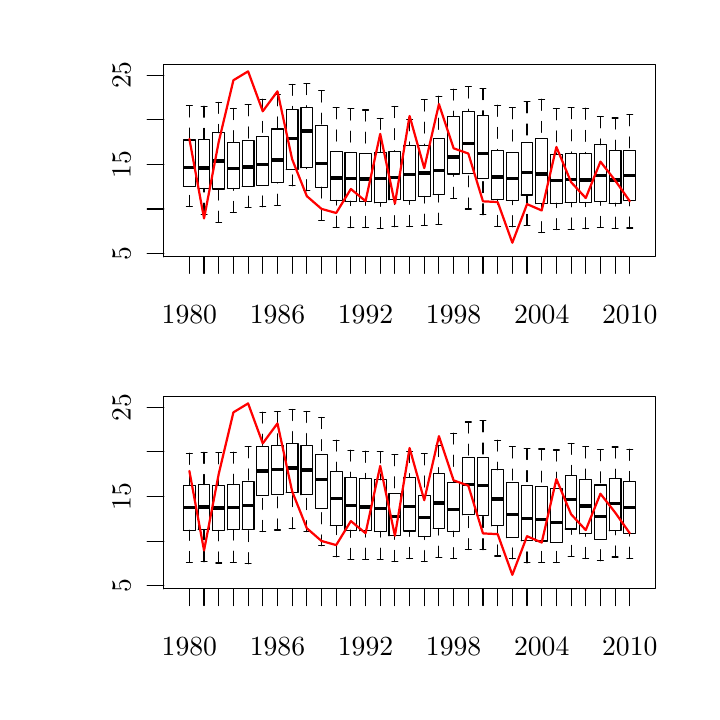
\begin{tikzpicture}[x=1pt,y=1pt]
\definecolor[named]{drawColor}{rgb}{0.00,0.00,0.00}
\definecolor[named]{fillColor}{rgb}{1.00,1.00,1.00}
\fill[color=fillColor,] (0,0) rectangle (240.00,240.00);
\begin{scope}
\path[clip] ( 49.20,157.20) rectangle (226.80,226.80);
\definecolor[named]{drawColor}{rgb}{0.00,0.00,0.00}

\draw[color=drawColor,line width= 1.2pt,line join=round,fill opacity=0.00,] ( 56.31,189.42) -- ( 60.55,189.42);

\draw[color=drawColor,dash pattern=on 4pt off 4pt ,line cap=round,line join=round,fill opacity=0.00,] ( 58.43,175.35) -- ( 58.43,182.73);

\draw[color=drawColor,dash pattern=on 4pt off 4pt ,line cap=round,line join=round,fill opacity=0.00,] ( 58.43,211.73) -- ( 58.43,199.42);

\draw[color=drawColor,line cap=round,line join=round,fill opacity=0.00,] ( 57.37,175.35) -- ( 59.49,175.35);

\draw[color=drawColor,line cap=round,line join=round,fill opacity=0.00,] ( 57.37,211.73) -- ( 59.49,211.73);

\draw[color=drawColor,line cap=round,line join=round,fill opacity=0.00,] ( 56.31,182.73) --
	( 60.55,182.73) --
	( 60.55,199.42) --
	( 56.31,199.42) --
	( 56.31,182.73);

\draw[color=drawColor,line width= 1.2pt,line join=round,fill opacity=0.00,] ( 61.61,189.30) -- ( 65.86,189.30);

\draw[color=drawColor,dash pattern=on 4pt off 4pt ,line cap=round,line join=round,fill opacity=0.00,] ( 63.73,172.61) -- ( 63.73,181.94);

\draw[color=drawColor,dash pattern=on 4pt off 4pt ,line cap=round,line join=round,fill opacity=0.00,] ( 63.73,211.61) -- ( 63.73,199.47);

\draw[color=drawColor,line cap=round,line join=round,fill opacity=0.00,] ( 62.67,172.61) -- ( 64.80,172.61);

\draw[color=drawColor,line cap=round,line join=round,fill opacity=0.00,] ( 62.67,211.61) -- ( 64.80,211.61);

\draw[color=drawColor,line cap=round,line join=round,fill opacity=0.00,] ( 61.61,181.94) --
	( 65.86,181.94) --
	( 65.86,199.47) --
	( 61.61,199.47) --
	( 61.61,181.94);

\draw[color=drawColor,line width= 1.2pt,line join=round,fill opacity=0.00,] ( 66.92,191.79) -- ( 71.16,191.79);

\draw[color=drawColor,dash pattern=on 4pt off 4pt ,line cap=round,line join=round,fill opacity=0.00,] ( 69.04,169.70) -- ( 69.04,181.72);

\draw[color=drawColor,dash pattern=on 4pt off 4pt ,line cap=round,line join=round,fill opacity=0.00,] ( 69.04,213.03) -- ( 69.04,202.04);

\draw[color=drawColor,line cap=round,line join=round,fill opacity=0.00,] ( 67.98,169.70) -- ( 70.10,169.70);

\draw[color=drawColor,line cap=round,line join=round,fill opacity=0.00,] ( 67.98,213.03) -- ( 70.10,213.03);

\draw[color=drawColor,line cap=round,line join=round,fill opacity=0.00,] ( 66.92,181.72) --
	( 71.16,181.72) --
	( 71.16,202.04) --
	( 66.92,202.04) --
	( 66.92,181.72);

\draw[color=drawColor,line width= 1.2pt,line join=round,fill opacity=0.00,] ( 72.22,189.19) -- ( 76.47,189.19);

\draw[color=drawColor,dash pattern=on 4pt off 4pt ,line cap=round,line join=round,fill opacity=0.00,] ( 74.34,173.23) -- ( 74.34,181.94);

\draw[color=drawColor,dash pattern=on 4pt off 4pt ,line cap=round,line join=round,fill opacity=0.00,] ( 74.34,210.81) -- ( 74.34,198.54);

\draw[color=drawColor,line cap=round,line join=round,fill opacity=0.00,] ( 73.28,173.23) -- ( 75.41,173.23);

\draw[color=drawColor,line cap=round,line join=round,fill opacity=0.00,] ( 73.28,210.81) -- ( 75.41,210.81);

\draw[color=drawColor,line cap=round,line join=round,fill opacity=0.00,] ( 72.22,181.94) --
	( 76.47,181.94) --
	( 76.47,198.54) --
	( 72.22,198.54) --
	( 72.22,181.94);

\draw[color=drawColor,line width= 1.2pt,line join=round,fill opacity=0.00,] ( 77.53,189.69) -- ( 81.77,189.69);

\draw[color=drawColor,dash pattern=on 4pt off 4pt ,line cap=round,line join=round,fill opacity=0.00,] ( 79.65,175.08) -- ( 79.65,182.67);

\draw[color=drawColor,dash pattern=on 4pt off 4pt ,line cap=round,line join=round,fill opacity=0.00,] ( 79.65,212.12) -- ( 79.65,199.13);

\draw[color=drawColor,line cap=round,line join=round,fill opacity=0.00,] ( 78.59,175.08) -- ( 80.71,175.08);

\draw[color=drawColor,line cap=round,line join=round,fill opacity=0.00,] ( 78.59,212.12) -- ( 80.71,212.12);

\draw[color=drawColor,line cap=round,line join=round,fill opacity=0.00,] ( 77.53,182.67) --
	( 81.77,182.67) --
	( 81.77,199.13) --
	( 77.53,199.13) --
	( 77.53,182.67);

\draw[color=drawColor,line width= 1.2pt,line join=round,fill opacity=0.00,] ( 82.83,190.49) -- ( 87.08,190.49);

\draw[color=drawColor,dash pattern=on 4pt off 4pt ,line cap=round,line join=round,fill opacity=0.00,] ( 84.95,175.23) -- ( 84.95,183.03);

\draw[color=drawColor,dash pattern=on 4pt off 4pt ,line cap=round,line join=round,fill opacity=0.00,] ( 84.95,214.15) -- ( 84.95,200.53);

\draw[color=drawColor,line cap=round,line join=round,fill opacity=0.00,] ( 83.89,175.23) -- ( 86.01,175.23);

\draw[color=drawColor,line cap=round,line join=round,fill opacity=0.00,] ( 83.89,214.15) -- ( 86.01,214.15);

\draw[color=drawColor,line cap=round,line join=round,fill opacity=0.00,] ( 82.83,183.03) --
	( 87.08,183.03) --
	( 87.08,200.53) --
	( 82.83,200.53) --
	( 82.83,183.03);

\draw[color=drawColor,line width= 1.2pt,line join=round,fill opacity=0.00,] ( 88.14,192.13) -- ( 92.38,192.13);

\draw[color=drawColor,dash pattern=on 4pt off 4pt ,line cap=round,line join=round,fill opacity=0.00,] ( 90.26,175.87) -- ( 90.26,184.00);

\draw[color=drawColor,dash pattern=on 4pt off 4pt ,line cap=round,line join=round,fill opacity=0.00,] ( 90.26,215.73) -- ( 90.26,203.37);

\draw[color=drawColor,line cap=round,line join=round,fill opacity=0.00,] ( 89.20,175.87) -- ( 91.32,175.87);

\draw[color=drawColor,line cap=round,line join=round,fill opacity=0.00,] ( 89.20,215.73) -- ( 91.32,215.73);

\draw[color=drawColor,line cap=round,line join=round,fill opacity=0.00,] ( 88.14,184.00) --
	( 92.38,184.00) --
	( 92.38,203.37) --
	( 88.14,203.37) --
	( 88.14,184.00);

\draw[color=drawColor,line width= 1.2pt,line join=round,fill opacity=0.00,] ( 93.44,199.97) -- ( 97.68,199.97);

\draw[color=drawColor,dash pattern=on 4pt off 4pt ,line cap=round,line join=round,fill opacity=0.00,] ( 95.56,182.82) -- ( 95.56,188.69);

\draw[color=drawColor,dash pattern=on 4pt off 4pt ,line cap=round,line join=round,fill opacity=0.00,] ( 95.56,219.52) -- ( 95.56,210.48);

\draw[color=drawColor,line cap=round,line join=round,fill opacity=0.00,] ( 94.50,182.82) -- ( 96.62,182.82);

\draw[color=drawColor,line cap=round,line join=round,fill opacity=0.00,] ( 94.50,219.52) -- ( 96.62,219.52);

\draw[color=drawColor,line cap=round,line join=round,fill opacity=0.00,] ( 93.44,188.69) --
	( 97.68,188.69) --
	( 97.68,210.48) --
	( 93.44,210.48) --
	( 93.44,188.69);

\draw[color=drawColor,line width= 1.2pt,line join=round,fill opacity=0.00,] ( 98.75,202.64) -- (102.99,202.64);

\draw[color=drawColor,dash pattern=on 4pt off 4pt ,line cap=round,line join=round,fill opacity=0.00,] (100.87,181.05) -- (100.87,189.39);

\draw[color=drawColor,dash pattern=on 4pt off 4pt ,line cap=round,line join=round,fill opacity=0.00,] (100.87,219.80) -- (100.87,211.16);

\draw[color=drawColor,line cap=round,line join=round,fill opacity=0.00,] ( 99.81,181.05) -- (101.93,181.05);

\draw[color=drawColor,line cap=round,line join=round,fill opacity=0.00,] ( 99.81,219.80) -- (101.93,219.80);

\draw[color=drawColor,line cap=round,line join=round,fill opacity=0.00,] ( 98.75,189.39) --
	(102.99,189.39) --
	(102.99,211.16) --
	( 98.75,211.16) --
	( 98.75,189.39);

\draw[color=drawColor,line width= 1.2pt,line join=round,fill opacity=0.00,] (104.05,190.99) -- (108.29,190.99);

\draw[color=drawColor,dash pattern=on 4pt off 4pt ,line cap=round,line join=round,fill opacity=0.00,] (106.17,170.41) -- (106.17,182.36);

\draw[color=drawColor,dash pattern=on 4pt off 4pt ,line cap=round,line join=round,fill opacity=0.00,] (106.17,217.14) -- (106.17,204.76);

\draw[color=drawColor,line cap=round,line join=round,fill opacity=0.00,] (105.11,170.41) -- (107.23,170.41);

\draw[color=drawColor,line cap=round,line join=round,fill opacity=0.00,] (105.11,217.14) -- (107.23,217.14);

\draw[color=drawColor,line cap=round,line join=round,fill opacity=0.00,] (104.05,182.36) --
	(108.29,182.36) --
	(108.29,204.76) --
	(104.05,204.76) --
	(104.05,182.36);

\draw[color=drawColor,line width= 1.2pt,line join=round,fill opacity=0.00,] (109.35,185.73) -- (113.60,185.73);

\draw[color=drawColor,dash pattern=on 4pt off 4pt ,line cap=round,line join=round,fill opacity=0.00,] (111.48,167.91) -- (111.48,177.62);

\draw[color=drawColor,dash pattern=on 4pt off 4pt ,line cap=round,line join=round,fill opacity=0.00,] (111.48,211.04) -- (111.48,195.19);

\draw[color=drawColor,line cap=round,line join=round,fill opacity=0.00,] (110.42,167.91) -- (112.54,167.91);

\draw[color=drawColor,line cap=round,line join=round,fill opacity=0.00,] (110.42,211.04) -- (112.54,211.04);

\draw[color=drawColor,line cap=round,line join=round,fill opacity=0.00,] (109.35,177.62) --
	(113.60,177.62) --
	(113.60,195.19) --
	(109.35,195.19) --
	(109.35,177.62);

\draw[color=drawColor,line width= 1.2pt,line join=round,fill opacity=0.00,] (114.66,185.39) -- (118.90,185.39);

\draw[color=drawColor,dash pattern=on 4pt off 4pt ,line cap=round,line join=round,fill opacity=0.00,] (116.78,167.71) -- (116.78,177.34);

\draw[color=drawColor,dash pattern=on 4pt off 4pt ,line cap=round,line join=round,fill opacity=0.00,] (116.78,210.63) -- (116.78,194.79);

\draw[color=drawColor,line cap=round,line join=round,fill opacity=0.00,] (115.72,167.71) -- (117.84,167.71);

\draw[color=drawColor,line cap=round,line join=round,fill opacity=0.00,] (115.72,210.63) -- (117.84,210.63);

\draw[color=drawColor,line cap=round,line join=round,fill opacity=0.00,] (114.66,177.34) --
	(118.90,177.34) --
	(118.90,194.79) --
	(114.66,194.79) --
	(114.66,177.34);

\draw[color=drawColor,line width= 1.2pt,line join=round,fill opacity=0.00,] (119.96,185.28) -- (124.21,185.28);

\draw[color=drawColor,dash pattern=on 4pt off 4pt ,line cap=round,line join=round,fill opacity=0.00,] (122.09,167.79) -- (122.09,177.32);

\draw[color=drawColor,dash pattern=on 4pt off 4pt ,line cap=round,line join=round,fill opacity=0.00,] (122.09,210.26) -- (122.09,194.55);

\draw[color=drawColor,line cap=round,line join=round,fill opacity=0.00,] (121.03,167.79) -- (123.15,167.79);

\draw[color=drawColor,line cap=round,line join=round,fill opacity=0.00,] (121.03,210.26) -- (123.15,210.26);

\draw[color=drawColor,line cap=round,line join=round,fill opacity=0.00,] (119.96,177.32) --
	(124.21,177.32) --
	(124.21,194.55) --
	(119.96,194.55) --
	(119.96,177.32);

\draw[color=drawColor,line width= 1.2pt,line join=round,fill opacity=0.00,] (125.27,185.59) -- (129.51,185.59);

\draw[color=drawColor,dash pattern=on 4pt off 4pt ,line cap=round,line join=round,fill opacity=0.00,] (127.39,167.43) -- (127.39,176.67);

\draw[color=drawColor,dash pattern=on 4pt off 4pt ,line cap=round,line join=round,fill opacity=0.00,] (127.39,207.25) -- (127.39,194.98);

\draw[color=drawColor,line cap=round,line join=round,fill opacity=0.00,] (126.33,167.43) -- (128.45,167.43);

\draw[color=drawColor,line cap=round,line join=round,fill opacity=0.00,] (126.33,207.25) -- (128.45,207.25);

\draw[color=drawColor,line cap=round,line join=round,fill opacity=0.00,] (125.27,176.67) --
	(129.51,176.67) --
	(129.51,194.98) --
	(125.27,194.98) --
	(125.27,176.67);

\draw[color=drawColor,line width= 1.2pt,line join=round,fill opacity=0.00,] (130.57,185.93) -- (134.82,185.93);

\draw[color=drawColor,dash pattern=on 4pt off 4pt ,line cap=round,line join=round,fill opacity=0.00,] (132.70,168.07) -- (132.70,177.81);

\draw[color=drawColor,dash pattern=on 4pt off 4pt ,line cap=round,line join=round,fill opacity=0.00,] (132.70,211.53) -- (132.70,195.29);

\draw[color=drawColor,line cap=round,line join=round,fill opacity=0.00,] (131.63,168.07) -- (133.76,168.07);

\draw[color=drawColor,line cap=round,line join=round,fill opacity=0.00,] (131.63,211.53) -- (133.76,211.53);

\draw[color=drawColor,line cap=round,line join=round,fill opacity=0.00,] (130.57,177.81) --
	(134.82,177.81) --
	(134.82,195.29) --
	(130.57,195.29) --
	(130.57,177.81);

\draw[color=drawColor,line width= 1.2pt,line join=round,fill opacity=0.00,] (135.88,186.95) -- (140.12,186.95);

\draw[color=drawColor,dash pattern=on 4pt off 4pt ,line cap=round,line join=round,fill opacity=0.00,] (138.00,168.16) -- (138.00,177.51);

\draw[color=drawColor,dash pattern=on 4pt off 4pt ,line cap=round,line join=round,fill opacity=0.00,] (138.00,206.70) -- (138.00,197.45);

\draw[color=drawColor,line cap=round,line join=round,fill opacity=0.00,] (136.94,168.16) -- (139.06,168.16);

\draw[color=drawColor,line cap=round,line join=round,fill opacity=0.00,] (136.94,206.70) -- (139.06,206.70);

\draw[color=drawColor,line cap=round,line join=round,fill opacity=0.00,] (135.88,177.51) --
	(140.12,177.51) --
	(140.12,197.45) --
	(135.88,197.45) --
	(135.88,177.51);

\draw[color=drawColor,line width= 1.2pt,line join=round,fill opacity=0.00,] (141.18,187.45) -- (145.43,187.45);

\draw[color=drawColor,dash pattern=on 4pt off 4pt ,line cap=round,line join=round,fill opacity=0.00,] (143.30,168.61) -- (143.30,179.06);

\draw[color=drawColor,dash pattern=on 4pt off 4pt ,line cap=round,line join=round,fill opacity=0.00,] (143.30,213.89) -- (143.30,197.37);

\draw[color=drawColor,line cap=round,line join=round,fill opacity=0.00,] (142.24,168.61) -- (144.37,168.61);

\draw[color=drawColor,line cap=round,line join=round,fill opacity=0.00,] (142.24,213.89) -- (144.37,213.89);

\draw[color=drawColor,line cap=round,line join=round,fill opacity=0.00,] (141.18,179.06) --
	(145.43,179.06) --
	(145.43,197.37) --
	(141.18,197.37) --
	(141.18,179.06);

\draw[color=drawColor,line width= 1.2pt,line join=round,fill opacity=0.00,] (146.49,188.40) -- (150.73,188.40);

\draw[color=drawColor,dash pattern=on 4pt off 4pt ,line cap=round,line join=round,fill opacity=0.00,] (148.61,169.01) -- (148.61,179.71);

\draw[color=drawColor,dash pattern=on 4pt off 4pt ,line cap=round,line join=round,fill opacity=0.00,] (148.61,215.28) -- (148.61,199.93);

\draw[color=drawColor,line cap=round,line join=round,fill opacity=0.00,] (147.55,169.01) -- (149.67,169.01);

\draw[color=drawColor,line cap=round,line join=round,fill opacity=0.00,] (147.55,215.28) -- (149.67,215.28);

\draw[color=drawColor,line cap=round,line join=round,fill opacity=0.00,] (146.49,179.71) --
	(150.73,179.71) --
	(150.73,199.93) --
	(146.49,199.93) --
	(146.49,179.71);

\draw[color=drawColor,line width= 1.2pt,line join=round,fill opacity=0.00,] (151.79,193.32) -- (156.04,193.32);

\draw[color=drawColor,dash pattern=on 4pt off 4pt ,line cap=round,line join=round,fill opacity=0.00,] (153.91,178.32) -- (153.91,187.12);

\draw[color=drawColor,dash pattern=on 4pt off 4pt ,line cap=round,line join=round,fill opacity=0.00,] (153.91,217.81) -- (153.91,208.01);

\draw[color=drawColor,line cap=round,line join=round,fill opacity=0.00,] (152.85,178.32) -- (154.97,178.32);

\draw[color=drawColor,line cap=round,line join=round,fill opacity=0.00,] (152.85,217.81) -- (154.97,217.81);

\draw[color=drawColor,line cap=round,line join=round,fill opacity=0.00,] (151.79,187.12) --
	(156.04,187.12) --
	(156.04,208.01) --
	(151.79,208.01) --
	(151.79,187.12);

\draw[color=drawColor,line width= 1.2pt,line join=round,fill opacity=0.00,] (157.10,198.03) -- (161.34,198.03);

\draw[color=drawColor,dash pattern=on 4pt off 4pt ,line cap=round,line join=round,fill opacity=0.00,] (159.22,174.47) -- (159.22,187.32);

\draw[color=drawColor,dash pattern=on 4pt off 4pt ,line cap=round,line join=round,fill opacity=0.00,] (159.22,218.58) -- (159.22,209.78);

\draw[color=drawColor,line cap=round,line join=round,fill opacity=0.00,] (158.16,174.47) -- (160.28,174.47);

\draw[color=drawColor,line cap=round,line join=round,fill opacity=0.00,] (158.16,218.58) -- (160.28,218.58);

\draw[color=drawColor,line cap=round,line join=round,fill opacity=0.00,] (157.10,187.32) --
	(161.34,187.32) --
	(161.34,209.78) --
	(157.10,209.78) --
	(157.10,187.32);

\draw[color=drawColor,line width= 1.2pt,line join=round,fill opacity=0.00,] (162.40,194.53) -- (166.65,194.53);

\draw[color=drawColor,dash pattern=on 4pt off 4pt ,line cap=round,line join=round,fill opacity=0.00,] (164.52,172.39) -- (164.52,185.57);

\draw[color=drawColor,dash pattern=on 4pt off 4pt ,line cap=round,line join=round,fill opacity=0.00,] (164.52,217.99) -- (164.52,208.21);

\draw[color=drawColor,line cap=round,line join=round,fill opacity=0.00,] (163.46,172.39) -- (165.58,172.39);

\draw[color=drawColor,line cap=round,line join=round,fill opacity=0.00,] (163.46,217.99) -- (165.58,217.99);

\draw[color=drawColor,line cap=round,line join=round,fill opacity=0.00,] (162.40,185.57) --
	(166.65,185.57) --
	(166.65,208.21) --
	(162.40,208.21) --
	(162.40,185.57);

\draw[color=drawColor,line width= 1.2pt,line join=round,fill opacity=0.00,] (167.71,186.09) -- (171.95,186.09);

\draw[color=drawColor,dash pattern=on 4pt off 4pt ,line cap=round,line join=round,fill opacity=0.00,] (169.83,168.18) -- (169.83,177.91);

\draw[color=drawColor,dash pattern=on 4pt off 4pt ,line cap=round,line join=round,fill opacity=0.00,] (169.83,211.98) -- (169.83,195.77);

\draw[color=drawColor,line cap=round,line join=round,fill opacity=0.00,] (168.77,168.18) -- (170.89,168.18);

\draw[color=drawColor,line cap=round,line join=round,fill opacity=0.00,] (168.77,211.98) -- (170.89,211.98);

\draw[color=drawColor,line cap=round,line join=round,fill opacity=0.00,] (167.71,177.91) --
	(171.95,177.91) --
	(171.95,195.77) --
	(167.71,195.77) --
	(167.71,177.91);

\draw[color=drawColor,line width= 1.2pt,line join=round,fill opacity=0.00,] (173.01,185.60) -- (177.25,185.60);

\draw[color=drawColor,dash pattern=on 4pt off 4pt ,line cap=round,line join=round,fill opacity=0.00,] (175.13,168.03) -- (175.13,177.59);

\draw[color=drawColor,dash pattern=on 4pt off 4pt ,line cap=round,line join=round,fill opacity=0.00,] (175.13,211.03) -- (175.13,195.05);

\draw[color=drawColor,line cap=round,line join=round,fill opacity=0.00,] (174.07,168.03) -- (176.19,168.03);

\draw[color=drawColor,line cap=round,line join=round,fill opacity=0.00,] (174.07,211.03) -- (176.19,211.03);

\draw[color=drawColor,line cap=round,line join=round,fill opacity=0.00,] (173.01,177.59) --
	(177.25,177.59) --
	(177.25,195.05) --
	(173.01,195.05) --
	(173.01,177.59);

\draw[color=drawColor,line width= 1.2pt,line join=round,fill opacity=0.00,] (178.32,187.76) -- (182.56,187.76);

\draw[color=drawColor,dash pattern=on 4pt off 4pt ,line cap=round,line join=round,fill opacity=0.00,] (180.44,168.54) -- (180.44,179.52);

\draw[color=drawColor,dash pattern=on 4pt off 4pt ,line cap=round,line join=round,fill opacity=0.00,] (180.44,213.21) -- (180.44,198.47);

\draw[color=drawColor,line cap=round,line join=round,fill opacity=0.00,] (179.38,168.54) -- (181.50,168.54);

\draw[color=drawColor,line cap=round,line join=round,fill opacity=0.00,] (179.38,213.21) -- (181.50,213.21);

\draw[color=drawColor,line cap=round,line join=round,fill opacity=0.00,] (178.32,179.52) --
	(182.56,179.52) --
	(182.56,198.47) --
	(178.32,198.47) --
	(178.32,179.52);

\draw[color=drawColor,line width= 1.2pt,line join=round,fill opacity=0.00,] (183.62,187.17) -- (187.86,187.17);

\draw[color=drawColor,dash pattern=on 4pt off 4pt ,line cap=round,line join=round,fill opacity=0.00,] (185.74,165.92) -- (185.74,176.42);

\draw[color=drawColor,dash pattern=on 4pt off 4pt ,line cap=round,line join=round,fill opacity=0.00,] (185.74,214.15) -- (185.74,199.84);

\draw[color=drawColor,line cap=round,line join=round,fill opacity=0.00,] (184.68,165.92) -- (186.80,165.92);

\draw[color=drawColor,line cap=round,line join=round,fill opacity=0.00,] (184.68,214.15) -- (186.80,214.15);

\draw[color=drawColor,line cap=round,line join=round,fill opacity=0.00,] (183.62,176.42) --
	(187.86,176.42) --
	(187.86,199.84) --
	(183.62,199.84) --
	(183.62,176.42);

\draw[color=drawColor,line width= 1.2pt,line join=round,fill opacity=0.00,] (188.92,184.66) -- (193.17,184.66);

\draw[color=drawColor,dash pattern=on 4pt off 4pt ,line cap=round,line join=round,fill opacity=0.00,] (191.05,167.02) -- (191.05,176.59);

\draw[color=drawColor,dash pattern=on 4pt off 4pt ,line cap=round,line join=round,fill opacity=0.00,] (191.05,210.73) -- (191.05,194.26);

\draw[color=drawColor,line cap=round,line join=round,fill opacity=0.00,] (189.99,167.02) -- (192.11,167.02);

\draw[color=drawColor,line cap=round,line join=round,fill opacity=0.00,] (189.99,210.73) -- (192.11,210.73);

\draw[color=drawColor,line cap=round,line join=round,fill opacity=0.00,] (188.92,176.59) --
	(193.17,176.59) --
	(193.17,194.26) --
	(188.92,194.26) --
	(188.92,176.59);

\draw[color=drawColor,line width= 1.2pt,line join=round,fill opacity=0.00,] (194.23,185.04) -- (198.47,185.04);

\draw[color=drawColor,dash pattern=on 4pt off 4pt ,line cap=round,line join=round,fill opacity=0.00,] (196.35,167.22) -- (196.35,176.89);

\draw[color=drawColor,dash pattern=on 4pt off 4pt ,line cap=round,line join=round,fill opacity=0.00,] (196.35,211.10) -- (196.35,194.64);

\draw[color=drawColor,line cap=round,line join=round,fill opacity=0.00,] (195.29,167.22) -- (197.41,167.22);

\draw[color=drawColor,line cap=round,line join=round,fill opacity=0.00,] (195.29,211.10) -- (197.41,211.10);

\draw[color=drawColor,line cap=round,line join=round,fill opacity=0.00,] (194.23,176.89) --
	(198.47,176.89) --
	(198.47,194.64) --
	(194.23,194.64) --
	(194.23,176.89);

\draw[color=drawColor,line width= 1.2pt,line join=round,fill opacity=0.00,] (199.53,184.97) -- (203.78,184.97);

\draw[color=drawColor,dash pattern=on 4pt off 4pt ,line cap=round,line join=round,fill opacity=0.00,] (201.66,167.31) -- (201.66,176.89);

\draw[color=drawColor,dash pattern=on 4pt off 4pt ,line cap=round,line join=round,fill opacity=0.00,] (201.66,210.90) -- (201.66,194.52);

\draw[color=drawColor,line cap=round,line join=round,fill opacity=0.00,] (200.59,167.31) -- (202.72,167.31);

\draw[color=drawColor,line cap=round,line join=round,fill opacity=0.00,] (200.59,210.90) -- (202.72,210.90);

\draw[color=drawColor,line cap=round,line join=round,fill opacity=0.00,] (199.53,176.89) --
	(203.78,176.89) --
	(203.78,194.52) --
	(199.53,194.52) --
	(199.53,176.89);

\draw[color=drawColor,line width= 1.2pt,line join=round,fill opacity=0.00,] (204.84,186.58) -- (209.08,186.58);

\draw[color=drawColor,dash pattern=on 4pt off 4pt ,line cap=round,line join=round,fill opacity=0.00,] (206.96,167.82) -- (206.96,177.20);

\draw[color=drawColor,dash pattern=on 4pt off 4pt ,line cap=round,line join=round,fill opacity=0.00,] (206.96,207.77) -- (206.96,197.70);

\draw[color=drawColor,line cap=round,line join=round,fill opacity=0.00,] (205.90,167.82) -- (208.02,167.82);

\draw[color=drawColor,line cap=round,line join=round,fill opacity=0.00,] (205.90,207.77) -- (208.02,207.77);

\draw[color=drawColor,line cap=round,line join=round,fill opacity=0.00,] (204.84,177.20) --
	(209.08,177.20) --
	(209.08,197.70) --
	(204.84,197.70) --
	(204.84,177.20);

\draw[color=drawColor,line width= 1.2pt,line join=round,fill opacity=0.00,] (210.14,184.97) -- (214.39,184.97);

\draw[color=drawColor,dash pattern=on 4pt off 4pt ,line cap=round,line join=round,fill opacity=0.00,] (212.27,167.54) -- (212.27,176.57);

\draw[color=drawColor,dash pattern=on 4pt off 4pt ,line cap=round,line join=round,fill opacity=0.00,] (212.27,207.35) -- (212.27,195.66);

\draw[color=drawColor,line cap=round,line join=round,fill opacity=0.00,] (211.20,167.54) -- (213.33,167.54);

\draw[color=drawColor,line cap=round,line join=round,fill opacity=0.00,] (211.20,207.35) -- (213.33,207.35);

\draw[color=drawColor,line cap=round,line join=round,fill opacity=0.00,] (210.14,176.57) --
	(214.39,176.57) --
	(214.39,195.66) --
	(210.14,195.66) --
	(210.14,176.57);

\draw[color=drawColor,line width= 1.2pt,line join=round,fill opacity=0.00,] (215.45,186.57) -- (219.69,186.57);

\draw[color=drawColor,dash pattern=on 4pt off 4pt ,line cap=round,line join=round,fill opacity=0.00,] (217.57,167.62) -- (217.57,177.56);

\draw[color=drawColor,dash pattern=on 4pt off 4pt ,line cap=round,line join=round,fill opacity=0.00,] (217.57,208.55) -- (217.57,195.54);

\draw[color=drawColor,line cap=round,line join=round,fill opacity=0.00,] (216.51,167.62) -- (218.63,167.62);

\draw[color=drawColor,line cap=round,line join=round,fill opacity=0.00,] (216.51,208.55) -- (218.63,208.55);

\draw[color=drawColor,line cap=round,line join=round,fill opacity=0.00,] (215.45,177.56) --
	(219.69,177.56) --
	(219.69,195.54) --
	(215.45,195.54) --
	(215.45,177.56);
\end{scope}
\begin{scope}
\path[clip] (  0.00,  0.00) rectangle (240.00,240.00);
\definecolor[named]{drawColor}{rgb}{0.00,0.00,0.00}

\draw[color=drawColor,line cap=round,line join=round,fill opacity=0.00,] ( 58.43,157.20) -- (217.57,157.20);

\draw[color=drawColor,line cap=round,line join=round,fill opacity=0.00,] ( 58.43,157.20) -- ( 58.43,151.20);

\draw[color=drawColor,line cap=round,line join=round,fill opacity=0.00,] ( 63.73,157.20) -- ( 63.73,151.20);

\draw[color=drawColor,line cap=round,line join=round,fill opacity=0.00,] ( 69.04,157.20) -- ( 69.04,151.20);

\draw[color=drawColor,line cap=round,line join=round,fill opacity=0.00,] ( 74.34,157.20) -- ( 74.34,151.20);

\draw[color=drawColor,line cap=round,line join=round,fill opacity=0.00,] ( 79.65,157.20) -- ( 79.65,151.20);

\draw[color=drawColor,line cap=round,line join=round,fill opacity=0.00,] ( 84.95,157.20) -- ( 84.95,151.20);

\draw[color=drawColor,line cap=round,line join=round,fill opacity=0.00,] ( 90.26,157.20) -- ( 90.26,151.20);

\draw[color=drawColor,line cap=round,line join=round,fill opacity=0.00,] ( 95.56,157.20) -- ( 95.56,151.20);

\draw[color=drawColor,line cap=round,line join=round,fill opacity=0.00,] (100.87,157.20) -- (100.87,151.20);

\draw[color=drawColor,line cap=round,line join=round,fill opacity=0.00,] (106.17,157.20) -- (106.17,151.20);

\draw[color=drawColor,line cap=round,line join=round,fill opacity=0.00,] (111.48,157.20) -- (111.48,151.20);

\draw[color=drawColor,line cap=round,line join=round,fill opacity=0.00,] (116.78,157.20) -- (116.78,151.20);

\draw[color=drawColor,line cap=round,line join=round,fill opacity=0.00,] (122.09,157.20) -- (122.09,151.20);

\draw[color=drawColor,line cap=round,line join=round,fill opacity=0.00,] (127.39,157.20) -- (127.39,151.20);

\draw[color=drawColor,line cap=round,line join=round,fill opacity=0.00,] (132.70,157.20) -- (132.70,151.20);

\draw[color=drawColor,line cap=round,line join=round,fill opacity=0.00,] (138.00,157.20) -- (138.00,151.20);

\draw[color=drawColor,line cap=round,line join=round,fill opacity=0.00,] (143.30,157.20) -- (143.30,151.20);

\draw[color=drawColor,line cap=round,line join=round,fill opacity=0.00,] (148.61,157.20) -- (148.61,151.20);

\draw[color=drawColor,line cap=round,line join=round,fill opacity=0.00,] (153.91,157.20) -- (153.91,151.20);

\draw[color=drawColor,line cap=round,line join=round,fill opacity=0.00,] (159.22,157.20) -- (159.22,151.20);

\draw[color=drawColor,line cap=round,line join=round,fill opacity=0.00,] (164.52,157.20) -- (164.52,151.20);

\draw[color=drawColor,line cap=round,line join=round,fill opacity=0.00,] (169.83,157.20) -- (169.83,151.20);

\draw[color=drawColor,line cap=round,line join=round,fill opacity=0.00,] (175.13,157.20) -- (175.13,151.20);

\draw[color=drawColor,line cap=round,line join=round,fill opacity=0.00,] (180.44,157.20) -- (180.44,151.20);

\draw[color=drawColor,line cap=round,line join=round,fill opacity=0.00,] (185.74,157.20) -- (185.74,151.20);

\draw[color=drawColor,line cap=round,line join=round,fill opacity=0.00,] (191.05,157.20) -- (191.05,151.20);

\draw[color=drawColor,line cap=round,line join=round,fill opacity=0.00,] (196.35,157.20) -- (196.35,151.20);

\draw[color=drawColor,line cap=round,line join=round,fill opacity=0.00,] (201.66,157.20) -- (201.66,151.20);

\draw[color=drawColor,line cap=round,line join=round,fill opacity=0.00,] (206.96,157.20) -- (206.96,151.20);

\draw[color=drawColor,line cap=round,line join=round,fill opacity=0.00,] (212.27,157.20) -- (212.27,151.20);

\draw[color=drawColor,line cap=round,line join=round,fill opacity=0.00,] (217.57,157.20) -- (217.57,151.20);

\node[color=drawColor,anchor=base,inner sep=0pt, outer sep=0pt, scale=  1.00] at ( 58.43,133.20) {1980%
};

\node[color=drawColor,anchor=base,inner sep=0pt, outer sep=0pt, scale=  1.00] at ( 90.26,133.20) {1986%
};

\node[color=drawColor,anchor=base,inner sep=0pt, outer sep=0pt, scale=  1.00] at (122.09,133.20) {1992%
};

\node[color=drawColor,anchor=base,inner sep=0pt, outer sep=0pt, scale=  1.00] at (153.91,133.20) {1998%
};

\node[color=drawColor,anchor=base,inner sep=0pt, outer sep=0pt, scale=  1.00] at (185.74,133.20) {2004%
};

\node[color=drawColor,anchor=base,inner sep=0pt, outer sep=0pt, scale=  1.00] at (217.57,133.20) {2010%
};

\draw[color=drawColor,line cap=round,line join=round,fill opacity=0.00,] ( 49.20,158.35) -- ( 49.20,222.85);

\draw[color=drawColor,line cap=round,line join=round,fill opacity=0.00,] ( 49.20,158.35) -- ( 43.20,158.35);

\draw[color=drawColor,line cap=round,line join=round,fill opacity=0.00,] ( 49.20,174.47) -- ( 43.20,174.47);

\draw[color=drawColor,line cap=round,line join=round,fill opacity=0.00,] ( 49.20,190.60) -- ( 43.20,190.60);

\draw[color=drawColor,line cap=round,line join=round,fill opacity=0.00,] ( 49.20,206.72) -- ( 43.20,206.72);

\draw[color=drawColor,line cap=round,line join=round,fill opacity=0.00,] ( 49.20,222.85) -- ( 43.20,222.85);

\node[rotate= 90.00,color=drawColor,anchor=base,inner sep=0pt, outer sep=0pt, scale=  1.00] at ( 37.20,158.35) {5%
};

\node[rotate= 90.00,color=drawColor,anchor=base,inner sep=0pt, outer sep=0pt, scale=  1.00] at ( 37.20,190.60) {15%
};

\node[rotate= 90.00,color=drawColor,anchor=base,inner sep=0pt, outer sep=0pt, scale=  1.00] at ( 37.20,222.85) {25%
};

\draw[color=drawColor,line cap=round,line join=round,fill opacity=0.00,] ( 49.20,157.20) --
	(226.80,157.20) --
	(226.80,226.80) --
	( 49.20,226.80) --
	( 49.20,157.20);
\end{scope}
\begin{scope}
\path[clip] ( 49.20,157.20) rectangle (226.80,226.80);
\definecolor[named]{drawColor}{rgb}{1.00,0.00,0.00}

\draw[color=drawColor,line width= 0.8pt,line cap=round,line join=round,fill opacity=0.00,] ( 58.43,199.82) --
	( 63.73,171.08) --
	( 69.04,198.76) --
	( 74.34,221.00) --
	( 79.65,224.22) --
	( 84.95,209.79) --
	( 90.26,217.00) --
	( 95.56,192.47) --
	(100.87,179.12) --
	(106.17,174.52) --
	(111.48,173.03) --
	(116.78,181.71) --
	(122.09,177.32) --
	(127.39,201.62) --
	(132.70,176.41) --
	(138.00,208.10) --
	(143.30,189.25) --
	(148.61,212.39) --
	(153.91,196.41) --
	(159.22,194.52) --
	(164.52,177.25) --
	(169.83,176.99) --
	(175.13,162.29) --
	(180.44,176.24) --
	(185.74,173.95) --
	(191.05,196.89) --
	(196.35,184.19) --
	(201.66,178.45) --
	(206.96,191.59) --
	(212.27,184.81) --
	(217.57,177.31);
\end{scope}
\begin{scope}
\path[clip] ( 49.20, 37.20) rectangle (226.80,106.80);
\end{scope}
\begin{scope}
\path[clip] ( 49.20, 37.20) rectangle (226.80,106.80);
\definecolor[named]{drawColor}{rgb}{0.00,0.00,0.00}

\draw[color=drawColor,line width= 1.2pt,line join=round,fill opacity=0.00,] ( 56.31, 66.51) -- ( 60.55, 66.51);

\draw[color=drawColor,dash pattern=on 4pt off 4pt ,line cap=round,line join=round,fill opacity=0.00,] ( 58.43, 46.78) -- ( 58.43, 58.42);

\draw[color=drawColor,dash pattern=on 4pt off 4pt ,line cap=round,line join=round,fill opacity=0.00,] ( 58.43, 86.24) -- ( 58.43, 74.60);

\draw[color=drawColor,line cap=round,line join=round,fill opacity=0.00,] ( 57.37, 46.78) -- ( 59.49, 46.78);

\draw[color=drawColor,line cap=round,line join=round,fill opacity=0.00,] ( 57.37, 86.24) -- ( 59.49, 86.24);

\draw[color=drawColor,line cap=round,line join=round,fill opacity=0.00,] ( 56.31, 58.42) --
	( 60.55, 58.42) --
	( 60.55, 74.60) --
	( 56.31, 74.60) --
	( 56.31, 58.42);

\draw[color=drawColor,line width= 1.2pt,line join=round,fill opacity=0.00,] ( 61.61, 66.78) -- ( 65.86, 66.78);

\draw[color=drawColor,dash pattern=on 4pt off 4pt ,line cap=round,line join=round,fill opacity=0.00,] ( 63.73, 47.01) -- ( 63.73, 58.67);

\draw[color=drawColor,dash pattern=on 4pt off 4pt ,line cap=round,line join=round,fill opacity=0.00,] ( 63.73, 86.56) -- ( 63.73, 74.89);

\draw[color=drawColor,line cap=round,line join=round,fill opacity=0.00,] ( 62.67, 47.01) -- ( 64.80, 47.01);

\draw[color=drawColor,line cap=round,line join=round,fill opacity=0.00,] ( 62.67, 86.56) -- ( 64.80, 86.56);

\draw[color=drawColor,line cap=round,line join=round,fill opacity=0.00,] ( 61.61, 58.67) --
	( 65.86, 58.67) --
	( 65.86, 74.89) --
	( 61.61, 74.89) --
	( 61.61, 58.67);

\draw[color=drawColor,line width= 1.2pt,line join=round,fill opacity=0.00,] ( 66.92, 66.46) -- ( 71.16, 66.46);

\draw[color=drawColor,dash pattern=on 4pt off 4pt ,line cap=round,line join=round,fill opacity=0.00,] ( 69.04, 46.57) -- ( 69.04, 58.30);

\draw[color=drawColor,dash pattern=on 4pt off 4pt ,line cap=round,line join=round,fill opacity=0.00,] ( 69.04, 86.37) -- ( 69.04, 74.62);

\draw[color=drawColor,line cap=round,line join=round,fill opacity=0.00,] ( 67.98, 46.57) -- ( 70.10, 46.57);

\draw[color=drawColor,line cap=round,line join=round,fill opacity=0.00,] ( 67.98, 86.37) -- ( 70.10, 86.37);

\draw[color=drawColor,line cap=round,line join=round,fill opacity=0.00,] ( 66.92, 58.30) --
	( 71.16, 58.30) --
	( 71.16, 74.62) --
	( 66.92, 74.62) --
	( 66.92, 58.30);

\draw[color=drawColor,line width= 1.2pt,line join=round,fill opacity=0.00,] ( 72.22, 66.71) -- ( 76.47, 66.71);

\draw[color=drawColor,dash pattern=on 4pt off 4pt ,line cap=round,line join=round,fill opacity=0.00,] ( 74.34, 46.81) -- ( 74.34, 58.54);

\draw[color=drawColor,dash pattern=on 4pt off 4pt ,line cap=round,line join=round,fill opacity=0.00,] ( 74.34, 86.62) -- ( 74.34, 74.87);

\draw[color=drawColor,line cap=round,line join=round,fill opacity=0.00,] ( 73.28, 46.81) -- ( 75.41, 46.81);

\draw[color=drawColor,line cap=round,line join=round,fill opacity=0.00,] ( 73.28, 86.62) -- ( 75.41, 86.62);

\draw[color=drawColor,line cap=round,line join=round,fill opacity=0.00,] ( 72.22, 58.54) --
	( 76.47, 58.54) --
	( 76.47, 74.87) --
	( 72.22, 74.87) --
	( 72.22, 58.54);

\draw[color=drawColor,line width= 1.2pt,line join=round,fill opacity=0.00,] ( 77.53, 67.40) -- ( 81.77, 67.40);

\draw[color=drawColor,dash pattern=on 4pt off 4pt ,line cap=round,line join=round,fill opacity=0.00,] ( 79.65, 46.26) -- ( 79.65, 58.72);

\draw[color=drawColor,dash pattern=on 4pt off 4pt ,line cap=round,line join=round,fill opacity=0.00,] ( 79.65, 88.55) -- ( 79.65, 76.07);

\draw[color=drawColor,line cap=round,line join=round,fill opacity=0.00,] ( 78.59, 46.26) -- ( 80.71, 46.26);

\draw[color=drawColor,line cap=round,line join=round,fill opacity=0.00,] ( 78.59, 88.55) -- ( 80.71, 88.55);

\draw[color=drawColor,line cap=round,line join=round,fill opacity=0.00,] ( 77.53, 58.72) --
	( 81.77, 58.72) --
	( 81.77, 76.07) --
	( 77.53, 76.07) --
	( 77.53, 58.72);

\draw[color=drawColor,line width= 1.2pt,line join=round,fill opacity=0.00,] ( 82.83, 79.86) -- ( 87.08, 79.86);

\draw[color=drawColor,dash pattern=on 4pt off 4pt ,line cap=round,line join=round,fill opacity=0.00,] ( 84.95, 57.91) -- ( 84.95, 70.93);

\draw[color=drawColor,dash pattern=on 4pt off 4pt ,line cap=round,line join=round,fill opacity=0.00,] ( 84.95,101.09) -- ( 84.95, 88.63);

\draw[color=drawColor,line cap=round,line join=round,fill opacity=0.00,] ( 83.89, 57.91) -- ( 86.01, 57.91);

\draw[color=drawColor,line cap=round,line join=round,fill opacity=0.00,] ( 83.89,101.09) -- ( 86.01,101.09);

\draw[color=drawColor,line cap=round,line join=round,fill opacity=0.00,] ( 82.83, 70.93) --
	( 87.08, 70.93) --
	( 87.08, 88.63) --
	( 82.83, 88.63) --
	( 82.83, 70.93);

\draw[color=drawColor,line width= 1.2pt,line join=round,fill opacity=0.00,] ( 88.14, 80.28) -- ( 92.38, 80.28);

\draw[color=drawColor,dash pattern=on 4pt off 4pt ,line cap=round,line join=round,fill opacity=0.00,] ( 90.26, 58.48) -- ( 90.26, 71.44);

\draw[color=drawColor,dash pattern=on 4pt off 4pt ,line cap=round,line join=round,fill opacity=0.00,] ( 90.26,101.25) -- ( 90.26, 88.94);

\draw[color=drawColor,line cap=round,line join=round,fill opacity=0.00,] ( 89.20, 58.48) -- ( 91.32, 58.48);

\draw[color=drawColor,line cap=round,line join=round,fill opacity=0.00,] ( 89.20,101.25) -- ( 91.32,101.25);

\draw[color=drawColor,line cap=round,line join=round,fill opacity=0.00,] ( 88.14, 71.44) --
	( 92.38, 71.44) --
	( 92.38, 88.94) --
	( 88.14, 88.94) --
	( 88.14, 71.44);

\draw[color=drawColor,line width= 1.2pt,line join=round,fill opacity=0.00,] ( 93.44, 80.93) -- ( 97.68, 80.93);

\draw[color=drawColor,dash pattern=on 4pt off 4pt ,line cap=round,line join=round,fill opacity=0.00,] ( 95.56, 58.94) -- ( 95.56, 72.03);

\draw[color=drawColor,dash pattern=on 4pt off 4pt ,line cap=round,line join=round,fill opacity=0.00,] ( 95.56,102.06) -- ( 95.56, 89.66);

\draw[color=drawColor,line cap=round,line join=round,fill opacity=0.00,] ( 94.50, 58.94) -- ( 96.62, 58.94);

\draw[color=drawColor,line cap=round,line join=round,fill opacity=0.00,] ( 94.50,102.06) -- ( 96.62,102.06);

\draw[color=drawColor,line cap=round,line join=round,fill opacity=0.00,] ( 93.44, 72.03) --
	( 97.68, 72.03) --
	( 97.68, 89.66) --
	( 93.44, 89.66) --
	( 93.44, 72.03);

\draw[color=drawColor,line width= 1.2pt,line join=round,fill opacity=0.00,] ( 98.75, 80.21) -- (102.99, 80.21);

\draw[color=drawColor,dash pattern=on 4pt off 4pt ,line cap=round,line join=round,fill opacity=0.00,] (100.87, 57.87) -- (100.87, 71.23);

\draw[color=drawColor,dash pattern=on 4pt off 4pt ,line cap=round,line join=round,fill opacity=0.00,] (100.87,101.34) -- (100.87, 88.93);

\draw[color=drawColor,line cap=round,line join=round,fill opacity=0.00,] ( 99.81, 57.87) -- (101.93, 57.87);

\draw[color=drawColor,line cap=round,line join=round,fill opacity=0.00,] ( 99.81,101.34) -- (101.93,101.34);

\draw[color=drawColor,line cap=round,line join=round,fill opacity=0.00,] ( 98.75, 71.23) --
	(102.99, 71.23) --
	(102.99, 88.93) --
	( 98.75, 88.93) --
	( 98.75, 71.23);

\draw[color=drawColor,line width= 1.2pt,line join=round,fill opacity=0.00,] (104.05, 76.61) -- (108.29, 76.61);

\draw[color=drawColor,dash pattern=on 4pt off 4pt ,line cap=round,line join=round,fill opacity=0.00,] (106.17, 52.74) -- (106.17, 66.39);

\draw[color=drawColor,dash pattern=on 4pt off 4pt ,line cap=round,line join=round,fill opacity=0.00,] (106.17, 99.16) -- (106.17, 85.78);

\draw[color=drawColor,line cap=round,line join=round,fill opacity=0.00,] (105.11, 52.74) -- (107.23, 52.74);

\draw[color=drawColor,line cap=round,line join=round,fill opacity=0.00,] (105.11, 99.16) -- (107.23, 99.16);

\draw[color=drawColor,line cap=round,line join=round,fill opacity=0.00,] (104.05, 66.39) --
	(108.29, 66.39) --
	(108.29, 85.78) --
	(104.05, 85.78) --
	(104.05, 66.39);

\draw[color=drawColor,line width= 1.2pt,line join=round,fill opacity=0.00,] (109.35, 69.89) -- (113.60, 69.89);

\draw[color=drawColor,dash pattern=on 4pt off 4pt ,line cap=round,line join=round,fill opacity=0.00,] (111.48, 48.80) -- (111.48, 60.07);

\draw[color=drawColor,dash pattern=on 4pt off 4pt ,line cap=round,line join=round,fill opacity=0.00,] (111.48, 90.97) -- (111.48, 79.74);

\draw[color=drawColor,line cap=round,line join=round,fill opacity=0.00,] (110.42, 48.80) -- (112.54, 48.80);

\draw[color=drawColor,line cap=round,line join=round,fill opacity=0.00,] (110.42, 90.97) -- (112.54, 90.97);

\draw[color=drawColor,line cap=round,line join=round,fill opacity=0.00,] (109.35, 60.07) --
	(113.60, 60.07) --
	(113.60, 79.74) --
	(109.35, 79.74) --
	(109.35, 60.07);

\draw[color=drawColor,line width= 1.2pt,line join=round,fill opacity=0.00,] (114.66, 67.36) -- (118.90, 67.36);

\draw[color=drawColor,dash pattern=on 4pt off 4pt ,line cap=round,line join=round,fill opacity=0.00,] (116.78, 47.87) -- (116.78, 58.41);

\draw[color=drawColor,dash pattern=on 4pt off 4pt ,line cap=round,line join=round,fill opacity=0.00,] (116.78, 87.37) -- (116.78, 77.53);

\draw[color=drawColor,line cap=round,line join=round,fill opacity=0.00,] (115.72, 47.87) -- (117.84, 47.87);

\draw[color=drawColor,line cap=round,line join=round,fill opacity=0.00,] (115.72, 87.37) -- (117.84, 87.37);

\draw[color=drawColor,line cap=round,line join=round,fill opacity=0.00,] (114.66, 58.41) --
	(118.90, 58.41) --
	(118.90, 77.53) --
	(114.66, 77.53) --
	(114.66, 58.41);

\draw[color=drawColor,line width= 1.2pt,line join=round,fill opacity=0.00,] (119.96, 66.76) -- (124.21, 66.76);

\draw[color=drawColor,dash pattern=on 4pt off 4pt ,line cap=round,line join=round,fill opacity=0.00,] (122.09, 47.90) -- (122.09, 58.19);

\draw[color=drawColor,dash pattern=on 4pt off 4pt ,line cap=round,line join=round,fill opacity=0.00,] (122.09, 86.97) -- (122.09, 76.96);

\draw[color=drawColor,line cap=round,line join=round,fill opacity=0.00,] (121.03, 47.90) -- (123.15, 47.90);

\draw[color=drawColor,line cap=round,line join=round,fill opacity=0.00,] (121.03, 86.97) -- (123.15, 86.97);

\draw[color=drawColor,line cap=round,line join=round,fill opacity=0.00,] (119.96, 58.19) --
	(124.21, 58.19) --
	(124.21, 76.96) --
	(119.96, 76.96) --
	(119.96, 58.19);

\draw[color=drawColor,line width= 1.2pt,line join=round,fill opacity=0.00,] (125.27, 66.31) -- (129.51, 66.31);

\draw[color=drawColor,dash pattern=on 4pt off 4pt ,line cap=round,line join=round,fill opacity=0.00,] (127.39, 47.90) -- (127.39, 57.95);

\draw[color=drawColor,dash pattern=on 4pt off 4pt ,line cap=round,line join=round,fill opacity=0.00,] (127.39, 86.71) -- (127.39, 76.64);

\draw[color=drawColor,line cap=round,line join=round,fill opacity=0.00,] (126.33, 47.90) -- (128.45, 47.90);

\draw[color=drawColor,line cap=round,line join=round,fill opacity=0.00,] (126.33, 86.71) -- (128.45, 86.71);

\draw[color=drawColor,line cap=round,line join=round,fill opacity=0.00,] (125.27, 57.95) --
	(129.51, 57.95) --
	(129.51, 76.64) --
	(125.27, 76.64) --
	(125.27, 57.95);

\draw[color=drawColor,line width= 1.2pt,line join=round,fill opacity=0.00,] (130.57, 63.40) -- (134.82, 63.40);

\draw[color=drawColor,dash pattern=on 4pt off 4pt ,line cap=round,line join=round,fill opacity=0.00,] (132.70, 47.10) -- (132.70, 56.41);

\draw[color=drawColor,dash pattern=on 4pt off 4pt ,line cap=round,line join=round,fill opacity=0.00,] (132.70, 85.71) -- (132.70, 71.79);

\draw[color=drawColor,line cap=round,line join=round,fill opacity=0.00,] (131.63, 47.10) -- (133.76, 47.10);

\draw[color=drawColor,line cap=round,line join=round,fill opacity=0.00,] (131.63, 85.71) -- (133.76, 85.71);

\draw[color=drawColor,line cap=round,line join=round,fill opacity=0.00,] (130.57, 56.41) --
	(134.82, 56.41) --
	(134.82, 71.79) --
	(130.57, 71.79) --
	(130.57, 56.41);

\draw[color=drawColor,line width= 1.2pt,line join=round,fill opacity=0.00,] (135.88, 66.90) -- (140.12, 66.90);

\draw[color=drawColor,dash pattern=on 4pt off 4pt ,line cap=round,line join=round,fill opacity=0.00,] (138.00, 48.19) -- (138.00, 58.13);

\draw[color=drawColor,dash pattern=on 4pt off 4pt ,line cap=round,line join=round,fill opacity=0.00,] (138.00, 86.86) -- (138.00, 77.56);

\draw[color=drawColor,line cap=round,line join=round,fill opacity=0.00,] (136.94, 48.19) -- (139.06, 48.19);

\draw[color=drawColor,line cap=round,line join=round,fill opacity=0.00,] (136.94, 86.86) -- (139.06, 86.86);

\draw[color=drawColor,line cap=round,line join=round,fill opacity=0.00,] (135.88, 58.13) --
	(140.12, 58.13) --
	(140.12, 77.56) --
	(135.88, 77.56) --
	(135.88, 58.13);

\draw[color=drawColor,line width= 1.2pt,line join=round,fill opacity=0.00,] (141.18, 62.90) -- (145.43, 62.90);

\draw[color=drawColor,dash pattern=on 4pt off 4pt ,line cap=round,line join=round,fill opacity=0.00,] (143.30, 47.06) -- (143.30, 56.15);

\draw[color=drawColor,dash pattern=on 4pt off 4pt ,line cap=round,line join=round,fill opacity=0.00,] (143.30, 85.99) -- (143.30, 70.83);

\draw[color=drawColor,line cap=round,line join=round,fill opacity=0.00,] (142.24, 47.06) -- (144.37, 47.06);

\draw[color=drawColor,line cap=round,line join=round,fill opacity=0.00,] (142.24, 85.99) -- (144.37, 85.99);

\draw[color=drawColor,line cap=round,line join=round,fill opacity=0.00,] (141.18, 56.15) --
	(145.43, 56.15) --
	(145.43, 70.83) --
	(141.18, 70.83) --
	(141.18, 56.15);

\draw[color=drawColor,line width= 1.2pt,line join=round,fill opacity=0.00,] (146.49, 68.27) -- (150.73, 68.27);

\draw[color=drawColor,dash pattern=on 4pt off 4pt ,line cap=round,line join=round,fill opacity=0.00,] (148.61, 48.63) -- (148.61, 59.08);

\draw[color=drawColor,dash pattern=on 4pt off 4pt ,line cap=round,line join=round,fill opacity=0.00,] (148.61, 89.04) -- (148.61, 79.06);

\draw[color=drawColor,line cap=round,line join=round,fill opacity=0.00,] (147.55, 48.63) -- (149.67, 48.63);

\draw[color=drawColor,line cap=round,line join=round,fill opacity=0.00,] (147.55, 89.04) -- (149.67, 89.04);

\draw[color=drawColor,line cap=round,line join=round,fill opacity=0.00,] (146.49, 59.08) --
	(150.73, 59.08) --
	(150.73, 79.06) --
	(146.49, 79.06) --
	(146.49, 59.08);

\draw[color=drawColor,line width= 1.2pt,line join=round,fill opacity=0.00,] (151.79, 65.82) -- (156.04, 65.82);

\draw[color=drawColor,dash pattern=on 4pt off 4pt ,line cap=round,line join=round,fill opacity=0.00,] (153.91, 48.13) -- (153.91, 58.06);

\draw[color=drawColor,dash pattern=on 4pt off 4pt ,line cap=round,line join=round,fill opacity=0.00,] (153.91, 93.51) -- (153.91, 75.69);

\draw[color=drawColor,line cap=round,line join=round,fill opacity=0.00,] (152.85, 48.13) -- (154.97, 48.13);

\draw[color=drawColor,line cap=round,line join=round,fill opacity=0.00,] (152.85, 93.51) -- (154.97, 93.51);

\draw[color=drawColor,line cap=round,line join=round,fill opacity=0.00,] (151.79, 58.06) --
	(156.04, 58.06) --
	(156.04, 75.69) --
	(151.79, 75.69) --
	(151.79, 58.06);

\draw[color=drawColor,line width= 1.2pt,line join=round,fill opacity=0.00,] (157.10, 74.91) -- (161.34, 74.91);

\draw[color=drawColor,dash pattern=on 4pt off 4pt ,line cap=round,line join=round,fill opacity=0.00,] (159.22, 51.37) -- (159.22, 63.96);

\draw[color=drawColor,dash pattern=on 4pt off 4pt ,line cap=round,line join=round,fill opacity=0.00,] (159.22, 97.52) -- (159.22, 84.56);

\draw[color=drawColor,line cap=round,line join=round,fill opacity=0.00,] (158.16, 51.37) -- (160.28, 51.37);

\draw[color=drawColor,line cap=round,line join=round,fill opacity=0.00,] (158.16, 97.52) -- (160.28, 97.52);

\draw[color=drawColor,line cap=round,line join=round,fill opacity=0.00,] (157.10, 63.96) --
	(161.34, 63.96) --
	(161.34, 84.56) --
	(157.10, 84.56) --
	(157.10, 63.96);

\draw[color=drawColor,line width= 1.2pt,line join=round,fill opacity=0.00,] (162.40, 74.46) -- (166.65, 74.46);

\draw[color=drawColor,dash pattern=on 4pt off 4pt ,line cap=round,line join=round,fill opacity=0.00,] (164.52, 51.36) -- (164.52, 63.81);

\draw[color=drawColor,dash pattern=on 4pt off 4pt ,line cap=round,line join=round,fill opacity=0.00,] (164.52, 97.94) -- (164.52, 84.54);

\draw[color=drawColor,line cap=round,line join=round,fill opacity=0.00,] (163.46, 51.36) -- (165.58, 51.36);

\draw[color=drawColor,line cap=round,line join=round,fill opacity=0.00,] (163.46, 97.94) -- (165.58, 97.94);

\draw[color=drawColor,line cap=round,line join=round,fill opacity=0.00,] (162.40, 63.81) --
	(166.65, 63.81) --
	(166.65, 84.54) --
	(162.40, 84.54) --
	(162.40, 63.81);

\draw[color=drawColor,line width= 1.2pt,line join=round,fill opacity=0.00,] (167.71, 69.69) -- (171.95, 69.69);

\draw[color=drawColor,dash pattern=on 4pt off 4pt ,line cap=round,line join=round,fill opacity=0.00,] (169.83, 49.09) -- (169.83, 59.99);

\draw[color=drawColor,dash pattern=on 4pt off 4pt ,line cap=round,line join=round,fill opacity=0.00,] (169.83, 90.96) -- (169.83, 80.23);

\draw[color=drawColor,line cap=round,line join=round,fill opacity=0.00,] (168.77, 49.09) -- (170.89, 49.09);

\draw[color=drawColor,line cap=round,line join=round,fill opacity=0.00,] (168.77, 90.96) -- (170.89, 90.96);

\draw[color=drawColor,line cap=round,line join=round,fill opacity=0.00,] (167.71, 59.99) --
	(171.95, 59.99) --
	(171.95, 80.23) --
	(167.71, 80.23) --
	(167.71, 59.99);

\draw[color=drawColor,line width= 1.2pt,line join=round,fill opacity=0.00,] (173.01, 64.06) -- (177.25, 64.06);

\draw[color=drawColor,dash pattern=on 4pt off 4pt ,line cap=round,line join=round,fill opacity=0.00,] (175.13, 48.05) -- (175.13, 55.70);

\draw[color=drawColor,dash pattern=on 4pt off 4pt ,line cap=round,line join=round,fill opacity=0.00,] (175.13, 88.51) -- (175.13, 75.59);

\draw[color=drawColor,line cap=round,line join=round,fill opacity=0.00,] (174.07, 48.05) -- (176.19, 48.05);

\draw[color=drawColor,line cap=round,line join=round,fill opacity=0.00,] (174.07, 88.51) -- (176.19, 88.51);

\draw[color=drawColor,line cap=round,line join=round,fill opacity=0.00,] (173.01, 55.70) --
	(177.25, 55.70) --
	(177.25, 75.59) --
	(173.01, 75.59) --
	(173.01, 55.70);

\draw[color=drawColor,line width= 1.2pt,line join=round,fill opacity=0.00,] (178.32, 62.64) -- (182.56, 62.64);

\draw[color=drawColor,dash pattern=on 4pt off 4pt ,line cap=round,line join=round,fill opacity=0.00,] (180.44, 46.59) -- (180.44, 54.58);

\draw[color=drawColor,dash pattern=on 4pt off 4pt ,line cap=round,line join=round,fill opacity=0.00,] (180.44, 87.95) -- (180.44, 74.48);

\draw[color=drawColor,line cap=round,line join=round,fill opacity=0.00,] (179.38, 46.59) -- (181.50, 46.59);

\draw[color=drawColor,line cap=round,line join=round,fill opacity=0.00,] (179.38, 87.95) -- (181.50, 87.95);

\draw[color=drawColor,line cap=round,line join=round,fill opacity=0.00,] (178.32, 54.58) --
	(182.56, 54.58) --
	(182.56, 74.48) --
	(178.32, 74.48) --
	(178.32, 54.58);

\draw[color=drawColor,line width= 1.2pt,line join=round,fill opacity=0.00,] (183.62, 62.31) -- (187.86, 62.31);

\draw[color=drawColor,dash pattern=on 4pt off 4pt ,line cap=round,line join=round,fill opacity=0.00,] (185.74, 46.77) -- (185.74, 54.50);

\draw[color=drawColor,dash pattern=on 4pt off 4pt ,line cap=round,line join=round,fill opacity=0.00,] (185.74, 87.76) -- (185.74, 74.29);

\draw[color=drawColor,line cap=round,line join=round,fill opacity=0.00,] (184.68, 46.77) -- (186.80, 46.77);

\draw[color=drawColor,line cap=round,line join=round,fill opacity=0.00,] (184.68, 87.76) -- (186.80, 87.76);

\draw[color=drawColor,line cap=round,line join=round,fill opacity=0.00,] (183.62, 54.50) --
	(187.86, 54.50) --
	(187.86, 74.29) --
	(183.62, 74.29) --
	(183.62, 54.50);

\draw[color=drawColor,line width= 1.2pt,line join=round,fill opacity=0.00,] (188.92, 61.18) -- (193.17, 61.18);

\draw[color=drawColor,dash pattern=on 4pt off 4pt ,line cap=round,line join=round,fill opacity=0.00,] (191.05, 46.71) -- (191.05, 54.02);

\draw[color=drawColor,dash pattern=on 4pt off 4pt ,line cap=round,line join=round,fill opacity=0.00,] (191.05, 87.38) -- (191.05, 73.45);

\draw[color=drawColor,line cap=round,line join=round,fill opacity=0.00,] (189.99, 46.71) -- (192.11, 46.71);

\draw[color=drawColor,line cap=round,line join=round,fill opacity=0.00,] (189.99, 87.38) -- (192.11, 87.38);

\draw[color=drawColor,line cap=round,line join=round,fill opacity=0.00,] (188.92, 54.02) --
	(193.17, 54.02) --
	(193.17, 73.45) --
	(188.92, 73.45) --
	(188.92, 54.02);

\draw[color=drawColor,line width= 1.2pt,line join=round,fill opacity=0.00,] (194.23, 69.47) -- (198.47, 69.47);

\draw[color=drawColor,dash pattern=on 4pt off 4pt ,line cap=round,line join=round,fill opacity=0.00,] (196.35, 48.93) -- (196.35, 58.84);

\draw[color=drawColor,dash pattern=on 4pt off 4pt ,line cap=round,line join=round,fill opacity=0.00,] (196.35, 89.79) -- (196.35, 78.33);

\draw[color=drawColor,line cap=round,line join=round,fill opacity=0.00,] (195.29, 48.93) -- (197.41, 48.93);

\draw[color=drawColor,line cap=round,line join=round,fill opacity=0.00,] (195.29, 89.79) -- (197.41, 89.79);

\draw[color=drawColor,line cap=round,line join=round,fill opacity=0.00,] (194.23, 58.84) --
	(198.47, 58.84) --
	(198.47, 78.33) --
	(194.23, 78.33) --
	(194.23, 58.84);

\draw[color=drawColor,line width= 1.2pt,line join=round,fill opacity=0.00,] (199.53, 67.19) -- (203.78, 67.19);

\draw[color=drawColor,dash pattern=on 4pt off 4pt ,line cap=round,line join=round,fill opacity=0.00,] (201.66, 48.16) -- (201.66, 57.13);

\draw[color=drawColor,dash pattern=on 4pt off 4pt ,line cap=round,line join=round,fill opacity=0.00,] (201.66, 88.51) -- (201.66, 76.86);

\draw[color=drawColor,line cap=round,line join=round,fill opacity=0.00,] (200.59, 48.16) -- (202.72, 48.16);

\draw[color=drawColor,line cap=round,line join=round,fill opacity=0.00,] (200.59, 88.51) -- (202.72, 88.51);

\draw[color=drawColor,line cap=round,line join=round,fill opacity=0.00,] (199.53, 57.13) --
	(203.78, 57.13) --
	(203.78, 76.86) --
	(199.53, 76.86) --
	(199.53, 57.13);

\draw[color=drawColor,line width= 1.2pt,line join=round,fill opacity=0.00,] (204.84, 63.34) -- (209.08, 63.34);

\draw[color=drawColor,dash pattern=on 4pt off 4pt ,line cap=round,line join=round,fill opacity=0.00,] (206.96, 47.35) -- (206.96, 55.16);

\draw[color=drawColor,dash pattern=on 4pt off 4pt ,line cap=round,line join=round,fill opacity=0.00,] (206.96, 87.52) -- (206.96, 74.75);

\draw[color=drawColor,line cap=round,line join=round,fill opacity=0.00,] (205.90, 47.35) -- (208.02, 47.35);

\draw[color=drawColor,line cap=round,line join=round,fill opacity=0.00,] (205.90, 87.52) -- (208.02, 87.52);

\draw[color=drawColor,line cap=round,line join=round,fill opacity=0.00,] (204.84, 55.16) --
	(209.08, 55.16) --
	(209.08, 74.75) --
	(204.84, 74.75) --
	(204.84, 55.16);

\draw[color=drawColor,line width= 1.2pt,line join=round,fill opacity=0.00,] (210.14, 68.11) -- (214.39, 68.11);

\draw[color=drawColor,dash pattern=on 4pt off 4pt ,line cap=round,line join=round,fill opacity=0.00,] (212.27, 48.72) -- (212.27, 58.16);

\draw[color=drawColor,dash pattern=on 4pt off 4pt ,line cap=round,line join=round,fill opacity=0.00,] (212.27, 88.46) -- (212.27, 77.14);

\draw[color=drawColor,line cap=round,line join=round,fill opacity=0.00,] (211.20, 48.72) -- (213.33, 48.72);

\draw[color=drawColor,line cap=round,line join=round,fill opacity=0.00,] (211.20, 88.46) -- (213.33, 88.46);

\draw[color=drawColor,line cap=round,line join=round,fill opacity=0.00,] (210.14, 58.16) --
	(214.39, 58.16) --
	(214.39, 77.14) --
	(210.14, 77.14) --
	(210.14, 58.16);

\draw[color=drawColor,line width= 1.2pt,line join=round,fill opacity=0.00,] (215.45, 66.71) -- (219.69, 66.71);

\draw[color=drawColor,dash pattern=on 4pt off 4pt ,line cap=round,line join=round,fill opacity=0.00,] (217.57, 48.26) -- (217.57, 57.25);

\draw[color=drawColor,dash pattern=on 4pt off 4pt ,line cap=round,line join=round,fill opacity=0.00,] (217.57, 87.68) -- (217.57, 76.14);

\draw[color=drawColor,line cap=round,line join=round,fill opacity=0.00,] (216.51, 48.26) -- (218.63, 48.26);

\draw[color=drawColor,line cap=round,line join=round,fill opacity=0.00,] (216.51, 87.68) -- (218.63, 87.68);

\draw[color=drawColor,line cap=round,line join=round,fill opacity=0.00,] (215.45, 57.25) --
	(219.69, 57.25) --
	(219.69, 76.14) --
	(215.45, 76.14) --
	(215.45, 57.25);
\end{scope}
\begin{scope}
\path[clip] (  0.00,  0.00) rectangle (240.00,240.00);
\definecolor[named]{drawColor}{rgb}{0.00,0.00,0.00}

\draw[color=drawColor,line cap=round,line join=round,fill opacity=0.00,] ( 58.43, 37.20) -- (217.57, 37.20);

\draw[color=drawColor,line cap=round,line join=round,fill opacity=0.00,] ( 58.43, 37.20) -- ( 58.43, 31.20);

\draw[color=drawColor,line cap=round,line join=round,fill opacity=0.00,] ( 63.73, 37.20) -- ( 63.73, 31.20);

\draw[color=drawColor,line cap=round,line join=round,fill opacity=0.00,] ( 69.04, 37.20) -- ( 69.04, 31.20);

\draw[color=drawColor,line cap=round,line join=round,fill opacity=0.00,] ( 74.34, 37.20) -- ( 74.34, 31.20);

\draw[color=drawColor,line cap=round,line join=round,fill opacity=0.00,] ( 79.65, 37.20) -- ( 79.65, 31.20);

\draw[color=drawColor,line cap=round,line join=round,fill opacity=0.00,] ( 84.95, 37.20) -- ( 84.95, 31.20);

\draw[color=drawColor,line cap=round,line join=round,fill opacity=0.00,] ( 90.26, 37.20) -- ( 90.26, 31.20);

\draw[color=drawColor,line cap=round,line join=round,fill opacity=0.00,] ( 95.56, 37.20) -- ( 95.56, 31.20);

\draw[color=drawColor,line cap=round,line join=round,fill opacity=0.00,] (100.87, 37.20) -- (100.87, 31.20);

\draw[color=drawColor,line cap=round,line join=round,fill opacity=0.00,] (106.17, 37.20) -- (106.17, 31.20);

\draw[color=drawColor,line cap=round,line join=round,fill opacity=0.00,] (111.48, 37.20) -- (111.48, 31.20);

\draw[color=drawColor,line cap=round,line join=round,fill opacity=0.00,] (116.78, 37.20) -- (116.78, 31.20);

\draw[color=drawColor,line cap=round,line join=round,fill opacity=0.00,] (122.09, 37.20) -- (122.09, 31.20);

\draw[color=drawColor,line cap=round,line join=round,fill opacity=0.00,] (127.39, 37.20) -- (127.39, 31.20);

\draw[color=drawColor,line cap=round,line join=round,fill opacity=0.00,] (132.70, 37.20) -- (132.70, 31.20);

\draw[color=drawColor,line cap=round,line join=round,fill opacity=0.00,] (138.00, 37.20) -- (138.00, 31.20);

\draw[color=drawColor,line cap=round,line join=round,fill opacity=0.00,] (143.30, 37.20) -- (143.30, 31.20);

\draw[color=drawColor,line cap=round,line join=round,fill opacity=0.00,] (148.61, 37.20) -- (148.61, 31.20);

\draw[color=drawColor,line cap=round,line join=round,fill opacity=0.00,] (153.91, 37.20) -- (153.91, 31.20);

\draw[color=drawColor,line cap=round,line join=round,fill opacity=0.00,] (159.22, 37.20) -- (159.22, 31.20);

\draw[color=drawColor,line cap=round,line join=round,fill opacity=0.00,] (164.52, 37.20) -- (164.52, 31.20);

\draw[color=drawColor,line cap=round,line join=round,fill opacity=0.00,] (169.83, 37.20) -- (169.83, 31.20);

\draw[color=drawColor,line cap=round,line join=round,fill opacity=0.00,] (175.13, 37.20) -- (175.13, 31.20);

\draw[color=drawColor,line cap=round,line join=round,fill opacity=0.00,] (180.44, 37.20) -- (180.44, 31.20);

\draw[color=drawColor,line cap=round,line join=round,fill opacity=0.00,] (185.74, 37.20) -- (185.74, 31.20);

\draw[color=drawColor,line cap=round,line join=round,fill opacity=0.00,] (191.05, 37.20) -- (191.05, 31.20);

\draw[color=drawColor,line cap=round,line join=round,fill opacity=0.00,] (196.35, 37.20) -- (196.35, 31.20);

\draw[color=drawColor,line cap=round,line join=round,fill opacity=0.00,] (201.66, 37.20) -- (201.66, 31.20);

\draw[color=drawColor,line cap=round,line join=round,fill opacity=0.00,] (206.96, 37.20) -- (206.96, 31.20);

\draw[color=drawColor,line cap=round,line join=round,fill opacity=0.00,] (212.27, 37.20) -- (212.27, 31.20);

\draw[color=drawColor,line cap=round,line join=round,fill opacity=0.00,] (217.57, 37.20) -- (217.57, 31.20);

\node[color=drawColor,anchor=base,inner sep=0pt, outer sep=0pt, scale=  1.00] at ( 58.43, 13.20) {1980%
};

\node[color=drawColor,anchor=base,inner sep=0pt, outer sep=0pt, scale=  1.00] at ( 90.26, 13.20) {1986%
};

\node[color=drawColor,anchor=base,inner sep=0pt, outer sep=0pt, scale=  1.00] at (122.09, 13.20) {1992%
};

\node[color=drawColor,anchor=base,inner sep=0pt, outer sep=0pt, scale=  1.00] at (153.91, 13.20) {1998%
};

\node[color=drawColor,anchor=base,inner sep=0pt, outer sep=0pt, scale=  1.00] at (185.74, 13.20) {2004%
};

\node[color=drawColor,anchor=base,inner sep=0pt, outer sep=0pt, scale=  1.00] at (217.57, 13.20) {2010%
};

\draw[color=drawColor,line cap=round,line join=round,fill opacity=0.00,] ( 49.20, 38.35) -- ( 49.20,102.85);

\draw[color=drawColor,line cap=round,line join=round,fill opacity=0.00,] ( 49.20, 38.35) -- ( 43.20, 38.35);

\draw[color=drawColor,line cap=round,line join=round,fill opacity=0.00,] ( 49.20, 54.47) -- ( 43.20, 54.47);

\draw[color=drawColor,line cap=round,line join=round,fill opacity=0.00,] ( 49.20, 70.60) -- ( 43.20, 70.60);

\draw[color=drawColor,line cap=round,line join=round,fill opacity=0.00,] ( 49.20, 86.72) -- ( 43.20, 86.72);

\draw[color=drawColor,line cap=round,line join=round,fill opacity=0.00,] ( 49.20,102.85) -- ( 43.20,102.85);

\node[rotate= 90.00,color=drawColor,anchor=base,inner sep=0pt, outer sep=0pt, scale=  1.00] at ( 37.20, 38.35) {5%
};

\node[rotate= 90.00,color=drawColor,anchor=base,inner sep=0pt, outer sep=0pt, scale=  1.00] at ( 37.20, 70.60) {15%
};

\node[rotate= 90.00,color=drawColor,anchor=base,inner sep=0pt, outer sep=0pt, scale=  1.00] at ( 37.20,102.85) {25%
};

\draw[color=drawColor,line cap=round,line join=round,fill opacity=0.00,] ( 49.20, 37.20) --
	(226.80, 37.20) --
	(226.80,106.80) --
	( 49.20,106.80) --
	( 49.20, 37.20);
\end{scope}
\begin{scope}
\path[clip] ( 49.20, 37.20) rectangle (226.80,106.80);
\definecolor[named]{drawColor}{rgb}{1.00,0.00,0.00}

\draw[color=drawColor,line width= 0.8pt,line cap=round,line join=round,fill opacity=0.00,] ( 58.43, 79.82) --
	( 63.73, 51.08) --
	( 69.04, 78.76) --
	( 74.34,101.00) --
	( 79.65,104.22) --
	( 84.95, 89.79) --
	( 90.26, 97.00) --
	( 95.56, 72.47) --
	(100.87, 59.12) --
	(106.17, 54.52) --
	(111.48, 53.03) --
	(116.78, 61.71) --
	(122.09, 57.32) --
	(127.39, 81.62) --
	(132.70, 56.41) --
	(138.00, 88.10) --
	(143.30, 69.25) --
	(148.61, 92.39) --
	(153.91, 76.41) --
	(159.22, 74.52) --
	(164.52, 57.25) --
	(169.83, 56.99) --
	(175.13, 42.29) --
	(180.44, 56.24) --
	(185.74, 53.95) --
	(191.05, 76.89) --
	(196.35, 64.19) --
	(201.66, 58.45) --
	(206.96, 71.59) --
	(212.27, 64.81) --
	(217.57, 57.31);
\end{scope}
\end{tikzpicture}

\noindent\includegraphics[width=20pc]{plots/hmm-sim-figure9.pdf}
\caption{One step ahead forecasts from 1980 to 2010 for the HM3G (Top) and the HM3N (Bottom) with the actual data (solid line).}\label{fig:fc3}
\end{figure}

\begin{figure}
\centering
%\noindent\input{plots/boxplot-skills.tex} 
\noindent\includegraphics[width=20pc]{plots/hmm-sim-figure10.pdf}
\caption{Boxplots of RPSS values for the forecast period 1980-2010. The horizontal line at 0 represents the skill of the climatological forecast.}\label{fig:rpss}
\end{figure}


\begin{figure}
\centering
%\noindent\input{plots/pdf-shift1984.tex} 
%\noindent\input{plots/pdf-shift2004.tex} 
\noindent\includegraphics[width=20pc]{plots/hmm-sim-figure11.pdf}
\noindent\includegraphics[width=20pc]{plots/hmm-sim-figure12.pdf}
\caption{Forecast Distributions for 1984 (Left) and 2004 (right).  The historical value is shown as a vertical line.}\label{fig:fcdist}
\end{figure}

%\begin{figure}
%\centering
%\noindent% Created by tikzDevice version 0.6.1 on 2011-07-13 12:08:12
% !TEX encoding = UTF-8 Unicode
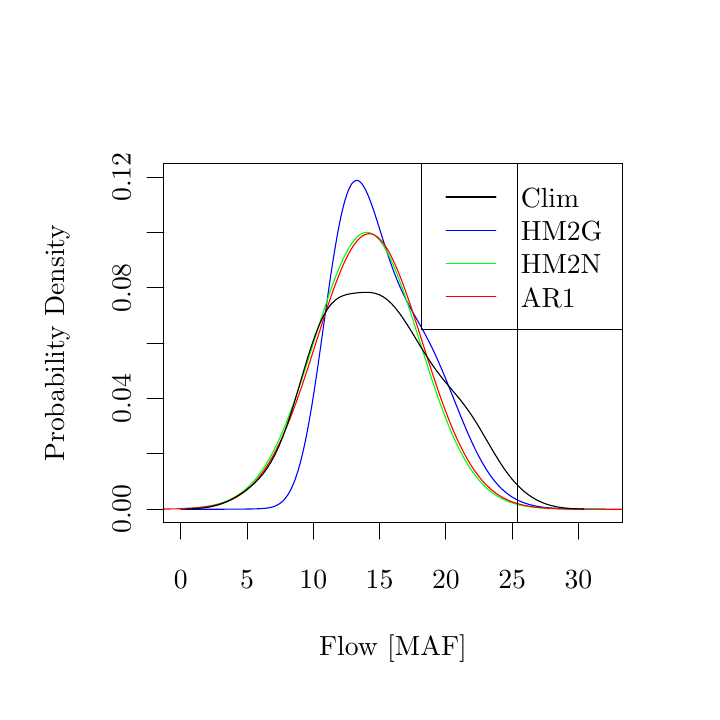
\begin{tikzpicture}[x=1pt,y=1pt]
\definecolor[named]{drawColor}{rgb}{0.00,0.00,0.00}
\definecolor[named]{fillColor}{rgb}{1.00,1.00,1.00}
\fill[color=fillColor,] (0,0) rectangle (240.00,240.00);
\begin{scope}
\path[clip] ( 49.20, 61.20) rectangle (214.80,190.80);
\definecolor[named]{drawColor}{rgb}{0.00,0.00,1.00}

\draw[color=drawColor,line cap=round,line join=round,fill opacity=0.00,] ( 55.33, 66.00) --
	( 55.64, 66.00) --
	( 55.95, 66.00) --
	( 56.26, 66.00) --
	( 56.56, 66.00) --
	( 56.87, 66.00) --
	( 57.18, 66.00) --
	( 57.48, 66.00) --
	( 57.79, 66.00) --
	( 58.10, 66.00) --
	( 58.41, 66.00) --
	( 58.71, 66.00) --
	( 59.02, 66.00) --
	( 59.33, 66.00) --
	( 59.64, 66.00) --
	( 59.94, 66.00) --
	( 60.25, 66.00) --
	( 60.56, 66.00) --
	( 60.86, 66.00) --
	( 61.17, 66.00) --
	( 61.48, 66.00) --
	( 61.79, 66.00) --
	( 62.09, 66.00) --
	( 62.40, 66.00) --
	( 62.71, 66.00) --
	( 63.02, 66.00) --
	( 63.32, 66.00) --
	( 63.63, 66.00) --
	( 63.94, 66.00) --
	( 64.24, 66.00) --
	( 64.55, 66.00) --
	( 64.86, 66.00) --
	( 65.17, 66.00) --
	( 65.47, 66.00) --
	( 65.78, 66.00) --
	( 66.09, 66.00) --
	( 66.40, 66.00) --
	( 66.70, 66.00) --
	( 67.01, 66.00) --
	( 67.32, 66.00) --
	( 67.62, 66.00) --
	( 67.93, 66.00) --
	( 68.24, 66.00) --
	( 68.55, 66.00) --
	( 68.85, 66.00) --
	( 69.16, 66.00) --
	( 69.47, 66.00) --
	( 69.78, 66.00) --
	( 70.08, 66.00) --
	( 70.39, 66.00) --
	( 70.70, 66.00) --
	( 71.00, 66.00) --
	( 71.31, 66.01) --
	( 71.62, 66.01) --
	( 71.93, 66.01) --
	( 72.23, 66.01) --
	( 72.54, 66.01) --
	( 72.85, 66.01) --
	( 73.16, 66.01) --
	( 73.46, 66.01) --
	( 73.77, 66.01) --
	( 74.08, 66.02) --
	( 74.38, 66.02) --
	( 74.69, 66.02) --
	( 75.00, 66.02) --
	( 75.31, 66.02) --
	( 75.61, 66.02) --
	( 75.92, 66.03) --
	( 76.23, 66.03) --
	( 76.54, 66.03) --
	( 76.84, 66.03) --
	( 77.15, 66.04) --
	( 77.46, 66.04) --
	( 77.76, 66.04) --
	( 78.07, 66.05) --
	( 78.38, 66.05) --
	( 78.69, 66.05) --
	( 78.99, 66.06) --
	( 79.30, 66.06) --
	( 79.61, 66.07) --
	( 79.92, 66.07) --
	( 80.22, 66.08) --
	( 80.53, 66.08) --
	( 80.84, 66.09) --
	( 81.14, 66.09) --
	( 81.45, 66.10) --
	( 81.76, 66.11) --
	( 82.07, 66.12) --
	( 82.37, 66.12) --
	( 82.68, 66.13) --
	( 82.99, 66.15) --
	( 83.30, 66.16) --
	( 83.60, 66.17) --
	( 83.91, 66.19) --
	( 84.22, 66.20) --
	( 84.53, 66.22) --
	( 84.83, 66.24) --
	( 85.14, 66.27) --
	( 85.45, 66.29) --
	( 85.75, 66.32) --
	( 86.06, 66.36) --
	( 86.37, 66.40) --
	( 86.68, 66.44) --
	( 86.98, 66.49) --
	( 87.29, 66.54) --
	( 87.60, 66.60) --
	( 87.91, 66.67) --
	( 88.21, 66.75) --
	( 88.52, 66.83) --
	( 88.83, 66.93) --
	( 89.13, 67.04) --
	( 89.44, 67.16) --
	( 89.75, 67.29) --
	( 90.06, 67.43) --
	( 90.36, 67.60) --
	( 90.67, 67.77) --
	( 90.98, 67.97) --
	( 91.29, 68.19) --
	( 91.59, 68.42) --
	( 91.90, 68.68) --
	( 92.21, 68.97) --
	( 92.51, 69.28) --
	( 92.82, 69.61) --
	( 93.13, 69.98) --
	( 93.44, 70.38) --
	( 93.74, 70.81) --
	( 94.05, 71.27) --
	( 94.36, 71.77) --
	( 94.67, 72.30) --
	( 94.97, 72.88) --
	( 95.28, 73.49) --
	( 95.59, 74.15) --
	( 95.89, 74.86) --
	( 96.20, 75.60) --
	( 96.51, 76.40) --
	( 96.82, 77.24) --
	( 97.12, 78.14) --
	( 97.43, 79.08) --
	( 97.74, 80.07) --
	( 98.05, 81.12) --
	( 98.35, 82.22) --
	( 98.66, 83.38) --
	( 98.97, 84.59) --
	( 99.27, 85.86) --
	( 99.58, 87.18) --
	( 99.89, 88.55) --
	(100.20, 89.98) --
	(100.50, 91.47) --
	(100.81, 93.01) --
	(101.12, 94.60) --
	(101.43, 96.25) --
	(101.73, 97.94) --
	(102.04, 99.69) --
	(102.35,101.48) --
	(102.65,103.32) --
	(102.96,105.21) --
	(103.27,107.13) --
	(103.58,109.10) --
	(103.88,111.10) --
	(104.19,113.14) --
	(104.50,115.21) --
	(104.81,117.31) --
	(105.11,119.44) --
	(105.42,121.58) --
	(105.73,123.75) --
	(106.03,125.93) --
	(106.34,128.12) --
	(106.65,130.32) --
	(106.96,132.52) --
	(107.26,134.72) --
	(107.57,136.92) --
	(107.88,139.11) --
	(108.19,141.28) --
	(108.49,143.44) --
	(108.80,145.58) --
	(109.11,147.69) --
	(109.41,149.78) --
	(109.72,151.83) --
	(110.03,153.85) --
	(110.34,155.82) --
	(110.64,157.76) --
	(110.95,159.64) --
	(111.26,161.48) --
	(111.57,163.26) --
	(111.87,164.98) --
	(112.18,166.65) --
	(112.49,168.25) --
	(112.79,169.79) --
	(113.10,171.26) --
	(113.41,172.66) --
	(113.72,173.99) --
	(114.02,175.24) --
	(114.33,176.42) --
	(114.64,177.53) --
	(114.95,178.55) --
	(115.25,179.50) --
	(115.56,180.37) --
	(115.87,181.16) --
	(116.18,181.88) --
	(116.48,182.51) --
	(116.79,183.06) --
	(117.10,183.54) --
	(117.40,183.94) --
	(117.71,184.26) --
	(118.02,184.50) --
	(118.33,184.67) --
	(118.63,184.77) --
	(118.94,184.79) --
	(119.25,184.75) --
	(119.56,184.64) --
	(119.86,184.46) --
	(120.17,184.21) --
	(120.48,183.91) --
	(120.78,183.55) --
	(121.09,183.13) --
	(121.40,182.65) --
	(121.71,182.13) --
	(122.01,181.56) --
	(122.32,180.94) --
	(122.63,180.28) --
	(122.94,179.57) --
	(123.24,178.83) --
	(123.55,178.06) --
	(123.86,177.25) --
	(124.16,176.42) --
	(124.47,175.56) --
	(124.78,174.67) --
	(125.09,173.77) --
	(125.39,172.84) --
	(125.70,171.90) --
	(126.01,170.95) --
	(126.32,169.99) --
	(126.62,169.02) --
	(126.93,168.04) --
	(127.24,167.06) --
	(127.54,166.08) --
	(127.85,165.10) --
	(128.16,164.12) --
	(128.47,163.15) --
	(128.77,162.18) --
	(129.08,161.22) --
	(129.39,160.27) --
	(129.70,159.32) --
	(130.00,158.39) --
	(130.31,157.47) --
	(130.62,156.57) --
	(130.92,155.67) --
	(131.23,154.80) --
	(131.54,153.93) --
	(131.85,153.08) --
	(132.15,152.25) --
	(132.46,151.44) --
	(132.77,150.64) --
	(133.08,149.86) --
	(133.38,149.09) --
	(133.69,148.34) --
	(134.00,147.61) --
	(134.30,146.89) --
	(134.61,146.19) --
	(134.92,145.50) --
	(135.23,144.83) --
	(135.53,144.17) --
	(135.84,143.52) --
	(136.15,142.89) --
	(136.46,142.27) --
	(136.76,141.66) --
	(137.07,141.06) --
	(137.38,140.47) --
	(137.68,139.88) --
	(137.99,139.31) --
	(138.30,138.75) --
	(138.61,138.19) --
	(138.91,137.63) --
	(139.22,137.08) --
	(139.53,136.53) --
	(139.84,135.99) --
	(140.14,135.45) --
	(140.45,134.91) --
	(140.76,134.37) --
	(141.06,133.83) --
	(141.37,133.28) --
	(141.68,132.74) --
	(141.99,132.19) --
	(142.29,131.64) --
	(142.60,131.09) --
	(142.91,130.53) --
	(143.22,129.96) --
	(143.52,129.39) --
	(143.83,128.82) --
	(144.14,128.24) --
	(144.44,127.65) --
	(144.75,127.05) --
	(145.06,126.45) --
	(145.37,125.84) --
	(145.67,125.22) --
	(145.98,124.59) --
	(146.29,123.96) --
	(146.60,123.31) --
	(146.90,122.66) --
	(147.21,122.00) --
	(147.52,121.33) --
	(147.82,120.66) --
	(148.13,119.97) --
	(148.44,119.28) --
	(148.75,118.58) --
	(149.05,117.87) --
	(149.36,117.16) --
	(149.67,116.44) --
	(149.98,115.71) --
	(150.28,114.98) --
	(150.59,114.24) --
	(150.90,113.50) --
	(151.21,112.75) --
	(151.51,112.00) --
	(151.82,111.24) --
	(152.13,110.48) --
	(152.43,109.71) --
	(152.74,108.95) --
	(153.05,108.18) --
	(153.36,107.41) --
	(153.66,106.64) --
	(153.97,105.87) --
	(154.28,105.09) --
	(154.59,104.32) --
	(154.89,103.55) --
	(155.20,102.79) --
	(155.51,102.02) --
	(155.81,101.26) --
	(156.12,100.49) --
	(156.43, 99.74) --
	(156.74, 98.98) --
	(157.04, 98.24) --
	(157.35, 97.49) --
	(157.66, 96.75) --
	(157.97, 96.02) --
	(158.27, 95.29) --
	(158.58, 94.58) --
	(158.89, 93.86) --
	(159.19, 93.16) --
	(159.50, 92.46) --
	(159.81, 91.77) --
	(160.12, 91.09) --
	(160.42, 90.42) --
	(160.73, 89.75) --
	(161.04, 89.10) --
	(161.35, 88.46) --
	(161.65, 87.82) --
	(161.96, 87.20) --
	(162.27, 86.58) --
	(162.57, 85.98) --
	(162.88, 85.38) --
	(163.19, 84.80) --
	(163.50, 84.23) --
	(163.80, 83.67) --
	(164.11, 83.12) --
	(164.42, 82.58) --
	(164.73, 82.05) --
	(165.03, 81.53) --
	(165.34, 81.03) --
	(165.65, 80.53) --
	(165.95, 80.05) --
	(166.26, 79.58) --
	(166.57, 79.11) --
	(166.88, 78.66) --
	(167.18, 78.23) --
	(167.49, 77.80) --
	(167.80, 77.38) --
	(168.11, 76.98) --
	(168.41, 76.58) --
	(168.72, 76.20) --
	(169.03, 75.82) --
	(169.33, 75.46) --
	(169.64, 75.10) --
	(169.95, 74.76) --
	(170.26, 74.43) --
	(170.56, 74.11) --
	(170.87, 73.79) --
	(171.18, 73.49) --
	(171.49, 73.19) --
	(171.79, 72.91) --
	(172.10, 72.63) --
	(172.41, 72.37) --
	(172.71, 72.11) --
	(173.02, 71.86) --
	(173.33, 71.62) --
	(173.64, 71.38) --
	(173.94, 71.16) --
	(174.25, 70.94) --
	(174.56, 70.73) --
	(174.87, 70.53) --
	(175.17, 70.33) --
	(175.48, 70.15) --
	(175.79, 69.96) --
	(176.09, 69.79) --
	(176.40, 69.62) --
	(176.71, 69.46) --
	(177.02, 69.31) --
	(177.32, 69.16) --
	(177.63, 69.01) --
	(177.94, 68.87) --
	(178.25, 68.74) --
	(178.55, 68.62) --
	(178.86, 68.49) --
	(179.17, 68.38) --
	(179.47, 68.26) --
	(179.78, 68.16) --
	(180.09, 68.05) --
	(180.40, 67.96) --
	(180.70, 67.86) --
	(181.01, 67.77) --
	(181.32, 67.68) --
	(181.63, 67.60) --
	(181.93, 67.52) --
	(182.24, 67.45) --
	(182.55, 67.37) --
	(182.86, 67.31) --
	(183.16, 67.24) --
	(183.47, 67.18) --
	(183.78, 67.12) --
	(184.08, 67.06) --
	(184.39, 67.00) --
	(184.70, 66.95) --
	(185.01, 66.90) --
	(185.31, 66.86) --
	(185.62, 66.81) --
	(185.93, 66.77) --
	(186.24, 66.73) --
	(186.54, 66.69) --
	(186.85, 66.65) --
	(187.16, 66.62) --
	(187.46, 66.58) --
	(187.77, 66.55) --
	(188.08, 66.52) --
	(188.39, 66.49) --
	(188.69, 66.47) --
	(189.00, 66.44) --
	(189.31, 66.42) --
	(189.62, 66.39) --
	(189.92, 66.37) --
	(190.23, 66.35) --
	(190.54, 66.33) --
	(190.84, 66.31) --
	(191.15, 66.29) --
	(191.46, 66.28) --
	(191.77, 66.26) --
	(192.07, 66.25) --
	(192.38, 66.23) --
	(192.69, 66.22) --
	(193.00, 66.20) --
	(193.30, 66.19) --
	(193.61, 66.18) --
	(193.92, 66.17) --
	(194.22, 66.16) --
	(194.53, 66.15) --
	(194.84, 66.14) --
	(195.15, 66.13) --
	(195.45, 66.13) --
	(195.76, 66.12) --
	(196.07, 66.11) --
	(196.38, 66.10) --
	(196.68, 66.10) --
	(196.99, 66.09) --
	(197.30, 66.09) --
	(197.60, 66.08) --
	(197.91, 66.08) --
	(198.22, 66.07) --
	(198.53, 66.07) --
	(198.83, 66.06) --
	(199.14, 66.06) --
	(199.45, 66.05) --
	(199.76, 66.05) --
	(200.06, 66.05) --
	(200.37, 66.05) --
	(200.68, 66.04) --
	(200.98, 66.04) --
	(201.29, 66.04) --
	(201.60, 66.03) --
	(201.91, 66.03) --
	(202.21, 66.03) --
	(202.52, 66.03) --
	(202.83, 66.03) --
	(203.14, 66.02) --
	(203.44, 66.02) --
	(203.75, 66.02) --
	(204.06, 66.02) --
	(204.36, 66.02) --
	(204.67, 66.02) --
	(204.98, 66.02) --
	(205.29, 66.02) --
	(205.59, 66.01) --
	(205.90, 66.01) --
	(206.21, 66.01) --
	(206.52, 66.01) --
	(206.82, 66.01) --
	(207.13, 66.01) --
	(207.44, 66.01) --
	(207.74, 66.01) --
	(208.05, 66.01) --
	(208.36, 66.01) --
	(208.67, 66.01);
\end{scope}
\begin{scope}
\path[clip] (  0.00,  0.00) rectangle (240.00,240.00);
\definecolor[named]{drawColor}{rgb}{0.00,0.00,0.00}

\draw[color=drawColor,line cap=round,line join=round,fill opacity=0.00,] ( 55.33, 61.20) -- (198.99, 61.20);

\draw[color=drawColor,line cap=round,line join=round,fill opacity=0.00,] ( 55.33, 61.20) -- ( 55.33, 55.20);

\draw[color=drawColor,line cap=round,line join=round,fill opacity=0.00,] ( 79.28, 61.20) -- ( 79.28, 55.20);

\draw[color=drawColor,line cap=round,line join=round,fill opacity=0.00,] (103.22, 61.20) -- (103.22, 55.20);

\draw[color=drawColor,line cap=round,line join=round,fill opacity=0.00,] (127.16, 61.20) -- (127.16, 55.20);

\draw[color=drawColor,line cap=round,line join=round,fill opacity=0.00,] (151.11, 61.20) -- (151.11, 55.20);

\draw[color=drawColor,line cap=round,line join=round,fill opacity=0.00,] (175.05, 61.20) -- (175.05, 55.20);

\draw[color=drawColor,line cap=round,line join=round,fill opacity=0.00,] (198.99, 61.20) -- (198.99, 55.20);

\node[color=drawColor,anchor=base,inner sep=0pt, outer sep=0pt, scale=  1.00] at ( 55.33, 37.20) {0%
};

\node[color=drawColor,anchor=base,inner sep=0pt, outer sep=0pt, scale=  1.00] at ( 79.28, 37.20) {5%
};

\node[color=drawColor,anchor=base,inner sep=0pt, outer sep=0pt, scale=  1.00] at (103.22, 37.20) {10%
};

\node[color=drawColor,anchor=base,inner sep=0pt, outer sep=0pt, scale=  1.00] at (127.16, 37.20) {15%
};

\node[color=drawColor,anchor=base,inner sep=0pt, outer sep=0pt, scale=  1.00] at (151.11, 37.20) {20%
};

\node[color=drawColor,anchor=base,inner sep=0pt, outer sep=0pt, scale=  1.00] at (175.05, 37.20) {25%
};

\node[color=drawColor,anchor=base,inner sep=0pt, outer sep=0pt, scale=  1.00] at (198.99, 37.20) {30%
};

\draw[color=drawColor,line cap=round,line join=round,fill opacity=0.00,] ( 49.20, 66.00) -- ( 49.20,186.00);

\draw[color=drawColor,line cap=round,line join=round,fill opacity=0.00,] ( 49.20, 66.00) -- ( 43.20, 66.00);

\draw[color=drawColor,line cap=round,line join=round,fill opacity=0.00,] ( 49.20, 86.00) -- ( 43.20, 86.00);

\draw[color=drawColor,line cap=round,line join=round,fill opacity=0.00,] ( 49.20,106.00) -- ( 43.20,106.00);

\draw[color=drawColor,line cap=round,line join=round,fill opacity=0.00,] ( 49.20,126.00) -- ( 43.20,126.00);

\draw[color=drawColor,line cap=round,line join=round,fill opacity=0.00,] ( 49.20,146.00) -- ( 43.20,146.00);

\draw[color=drawColor,line cap=round,line join=round,fill opacity=0.00,] ( 49.20,166.00) -- ( 43.20,166.00);

\draw[color=drawColor,line cap=round,line join=round,fill opacity=0.00,] ( 49.20,186.00) -- ( 43.20,186.00);

\node[rotate= 90.00,color=drawColor,anchor=base,inner sep=0pt, outer sep=0pt, scale=  1.00] at ( 37.20, 66.00) {0.00%
};

\node[rotate= 90.00,color=drawColor,anchor=base,inner sep=0pt, outer sep=0pt, scale=  1.00] at ( 37.20,106.00) {0.04%
};

\node[rotate= 90.00,color=drawColor,anchor=base,inner sep=0pt, outer sep=0pt, scale=  1.00] at ( 37.20,146.00) {0.08%
};

\node[rotate= 90.00,color=drawColor,anchor=base,inner sep=0pt, outer sep=0pt, scale=  1.00] at ( 37.20,186.00) {0.12%
};

\draw[color=drawColor,line cap=round,line join=round,fill opacity=0.00,] ( 49.20, 61.20) --
	(214.80, 61.20) --
	(214.80,190.80) --
	( 49.20,190.80) --
	( 49.20, 61.20);
\end{scope}
\begin{scope}
\path[clip] (  0.00,  0.00) rectangle (240.00,240.00);
\definecolor[named]{drawColor}{rgb}{0.00,0.00,0.00}

\node[color=drawColor,anchor=base,inner sep=0pt, outer sep=0pt, scale=  1.00] at (132.00, 13.20) {Flow [MAF]%
};

\node[rotate= 90.00,color=drawColor,anchor=base,inner sep=0pt, outer sep=0pt, scale=  1.00] at ( 13.20,126.00) {Probability Density%
};
\end{scope}
\begin{scope}
\path[clip] ( 49.20, 61.20) rectangle (214.80,190.80);
\definecolor[named]{drawColor}{rgb}{0.00,1.00,0.00}

\draw[color=drawColor,line cap=round,line join=round,fill opacity=0.00,] ( 55.33, 66.20) --
	( 55.64, 66.22) --
	( 55.95, 66.23) --
	( 56.26, 66.24) --
	( 56.56, 66.26) --
	( 56.87, 66.27) --
	( 57.18, 66.29) --
	( 57.48, 66.30) --
	( 57.79, 66.32) --
	( 58.10, 66.34) --
	( 58.41, 66.36) --
	( 58.71, 66.38) --
	( 59.02, 66.40) --
	( 59.33, 66.42) --
	( 59.64, 66.44) --
	( 59.94, 66.46) --
	( 60.25, 66.49) --
	( 60.56, 66.52) --
	( 60.86, 66.54) --
	( 61.17, 66.57) --
	( 61.48, 66.60) --
	( 61.79, 66.63) --
	( 62.09, 66.67) --
	( 62.40, 66.70) --
	( 62.71, 66.74) --
	( 63.02, 66.78) --
	( 63.32, 66.82) --
	( 63.63, 66.86) --
	( 63.94, 66.90) --
	( 64.24, 66.95) --
	( 64.55, 66.99) --
	( 64.86, 67.04) --
	( 65.17, 67.10) --
	( 65.47, 67.15) --
	( 65.78, 67.21) --
	( 66.09, 67.27) --
	( 66.40, 67.33) --
	( 66.70, 67.39) --
	( 67.01, 67.46) --
	( 67.32, 67.53) --
	( 67.62, 67.60) --
	( 67.93, 67.68) --
	( 68.24, 67.75) --
	( 68.55, 67.84) --
	( 68.85, 67.92) --
	( 69.16, 68.01) --
	( 69.47, 68.10) --
	( 69.78, 68.20) --
	( 70.08, 68.30) --
	( 70.39, 68.40) --
	( 70.70, 68.51) --
	( 71.00, 68.62) --
	( 71.31, 68.74) --
	( 71.62, 68.86) --
	( 71.93, 68.98) --
	( 72.23, 69.11) --
	( 72.54, 69.25) --
	( 72.85, 69.38) --
	( 73.16, 69.53) --
	( 73.46, 69.68) --
	( 73.77, 69.83) --
	( 74.08, 69.99) --
	( 74.38, 70.16) --
	( 74.69, 70.33) --
	( 75.00, 70.51) --
	( 75.31, 70.69) --
	( 75.61, 70.88) --
	( 75.92, 71.08) --
	( 76.23, 71.28) --
	( 76.54, 71.49) --
	( 76.84, 71.71) --
	( 77.15, 71.93) --
	( 77.46, 72.16) --
	( 77.76, 72.40) --
	( 78.07, 72.64) --
	( 78.38, 72.90) --
	( 78.69, 73.16) --
	( 78.99, 73.42) --
	( 79.30, 73.70) --
	( 79.61, 73.99) --
	( 79.92, 74.28) --
	( 80.22, 74.58) --
	( 80.53, 74.89) --
	( 80.84, 75.21) --
	( 81.14, 75.54) --
	( 81.45, 75.87) --
	( 81.76, 76.22) --
	( 82.07, 76.58) --
	( 82.37, 76.94) --
	( 82.68, 77.32) --
	( 82.99, 77.70) --
	( 83.30, 78.10) --
	( 83.60, 78.50) --
	( 83.91, 78.92) --
	( 84.22, 79.34) --
	( 84.53, 79.78) --
	( 84.83, 80.23) --
	( 85.14, 80.68) --
	( 85.45, 81.15) --
	( 85.75, 81.63) --
	( 86.06, 82.12) --
	( 86.37, 82.62) --
	( 86.68, 83.13) --
	( 86.98, 83.66) --
	( 87.29, 84.19) --
	( 87.60, 84.74) --
	( 87.91, 85.30) --
	( 88.21, 85.87) --
	( 88.52, 86.45) --
	( 88.83, 87.04) --
	( 89.13, 87.64) --
	( 89.44, 88.26) --
	( 89.75, 88.88) --
	( 90.06, 89.52) --
	( 90.36, 90.17) --
	( 90.67, 90.83) --
	( 90.98, 91.50) --
	( 91.29, 92.19) --
	( 91.59, 92.88) --
	( 91.90, 93.59) --
	( 92.21, 94.31) --
	( 92.51, 95.04) --
	( 92.82, 95.78) --
	( 93.13, 96.53) --
	( 93.44, 97.29) --
	( 93.74, 98.06) --
	( 94.05, 98.85) --
	( 94.36, 99.64) --
	( 94.67,100.44) --
	( 94.97,101.26) --
	( 95.28,102.08) --
	( 95.59,102.92) --
	( 95.89,103.76) --
	( 96.20,104.61) --
	( 96.51,105.47) --
	( 96.82,106.34) --
	( 97.12,107.22) --
	( 97.43,108.11) --
	( 97.74,109.01) --
	( 98.05,109.91) --
	( 98.35,110.82) --
	( 98.66,111.74) --
	( 98.97,112.66) --
	( 99.27,113.59) --
	( 99.58,114.53) --
	( 99.89,115.47) --
	(100.20,116.41) --
	(100.50,117.37) --
	(100.81,118.32) --
	(101.12,119.28) --
	(101.43,120.25) --
	(101.73,121.21) --
	(102.04,122.18) --
	(102.35,123.15) --
	(102.65,124.13) --
	(102.96,125.10) --
	(103.27,126.08) --
	(103.58,127.05) --
	(103.88,128.03) --
	(104.19,129.00) --
	(104.50,129.98) --
	(104.81,130.95) --
	(105.11,131.92) --
	(105.42,132.89) --
	(105.73,133.85) --
	(106.03,134.81) --
	(106.34,135.77) --
	(106.65,136.72) --
	(106.96,137.66) --
	(107.26,138.60) --
	(107.57,139.53) --
	(107.88,140.45) --
	(108.19,141.37) --
	(108.49,142.28) --
	(108.80,143.18) --
	(109.11,144.07) --
	(109.41,144.95) --
	(109.72,145.81) --
	(110.03,146.67) --
	(110.34,147.52) --
	(110.64,148.35) --
	(110.95,149.17) --
	(111.26,149.97) --
	(111.57,150.76) --
	(111.87,151.54) --
	(112.18,152.30) --
	(112.49,153.05) --
	(112.79,153.78) --
	(113.10,154.49) --
	(113.41,155.19) --
	(113.72,155.87) --
	(114.02,156.53) --
	(114.33,157.17) --
	(114.64,157.79) --
	(114.95,158.39) --
	(115.25,158.97) --
	(115.56,159.53) --
	(115.87,160.08) --
	(116.18,160.59) --
	(116.48,161.09) --
	(116.79,161.57) --
	(117.10,162.02) --
	(117.40,162.45) --
	(117.71,162.86) --
	(118.02,163.24) --
	(118.33,163.60) --
	(118.63,163.93) --
	(118.94,164.25) --
	(119.25,164.53) --
	(119.56,164.79) --
	(119.86,165.03) --
	(120.17,165.24) --
	(120.48,165.43) --
	(120.78,165.59) --
	(121.09,165.73) --
	(121.40,165.84) --
	(121.71,165.92) --
	(122.01,165.98) --
	(122.32,166.01) --
	(122.63,166.02) --
	(122.94,166.00) --
	(123.24,165.96) --
	(123.55,165.88) --
	(123.86,165.79) --
	(124.16,165.67) --
	(124.47,165.52) --
	(124.78,165.34) --
	(125.09,165.15) --
	(125.39,164.92) --
	(125.70,164.67) --
	(126.01,164.40) --
	(126.32,164.10) --
	(126.62,163.78) --
	(126.93,163.43) --
	(127.24,163.06) --
	(127.54,162.66) --
	(127.85,162.25) --
	(128.16,161.81) --
	(128.47,161.34) --
	(128.77,160.86) --
	(129.08,160.35) --
	(129.39,159.82) --
	(129.70,159.27) --
	(130.00,158.70) --
	(130.31,158.11) --
	(130.62,157.49) --
	(130.92,156.86) --
	(131.23,156.21) --
	(131.54,155.54) --
	(131.85,154.86) --
	(132.15,154.15) --
	(132.46,153.43) --
	(132.77,152.69) --
	(133.08,151.94) --
	(133.38,151.17) --
	(133.69,150.39) --
	(134.00,149.59) --
	(134.30,148.78) --
	(134.61,147.95) --
	(134.92,147.11) --
	(135.23,146.26) --
	(135.53,145.40) --
	(135.84,144.53) --
	(136.15,143.64) --
	(136.46,142.75) --
	(136.76,141.84) --
	(137.07,140.93) --
	(137.38,140.01) --
	(137.68,139.08) --
	(137.99,138.15) --
	(138.30,137.21) --
	(138.61,136.26) --
	(138.91,135.31) --
	(139.22,134.35) --
	(139.53,133.39) --
	(139.84,132.42) --
	(140.14,131.46) --
	(140.45,130.49) --
	(140.76,129.51) --
	(141.06,128.54) --
	(141.37,127.56) --
	(141.68,126.59) --
	(141.99,125.61) --
	(142.29,124.64) --
	(142.60,123.66) --
	(142.91,122.69) --
	(143.22,121.72) --
	(143.52,120.75) --
	(143.83,119.78) --
	(144.14,118.82) --
	(144.44,117.86) --
	(144.75,116.91) --
	(145.06,115.96) --
	(145.37,115.02) --
	(145.67,114.08) --
	(145.98,113.14) --
	(146.29,112.22) --
	(146.60,111.30) --
	(146.90,110.38) --
	(147.21,109.47) --
	(147.52,108.58) --
	(147.82,107.68) --
	(148.13,106.80) --
	(148.44,105.93) --
	(148.75,105.06) --
	(149.05,104.20) --
	(149.36,103.36) --
	(149.67,102.52) --
	(149.98,101.69) --
	(150.28,100.87) --
	(150.59,100.06) --
	(150.90, 99.26) --
	(151.21, 98.47) --
	(151.51, 97.69) --
	(151.82, 96.92) --
	(152.13, 96.17) --
	(152.43, 95.42) --
	(152.74, 94.69) --
	(153.05, 93.96) --
	(153.36, 93.25) --
	(153.66, 92.55) --
	(153.97, 91.86) --
	(154.28, 91.18) --
	(154.59, 90.51) --
	(154.89, 89.86) --
	(155.20, 89.21) --
	(155.51, 88.58) --
	(155.81, 87.96) --
	(156.12, 87.35) --
	(156.43, 86.75) --
	(156.74, 86.17) --
	(157.04, 85.59) --
	(157.35, 85.03) --
	(157.66, 84.48) --
	(157.97, 83.94) --
	(158.27, 83.41) --
	(158.58, 82.89) --
	(158.89, 82.38) --
	(159.19, 81.89) --
	(159.50, 81.40) --
	(159.81, 80.93) --
	(160.12, 80.46) --
	(160.42, 80.01) --
	(160.73, 79.57) --
	(161.04, 79.14) --
	(161.35, 78.72) --
	(161.65, 78.31) --
	(161.96, 77.91) --
	(162.27, 77.52) --
	(162.57, 77.14) --
	(162.88, 76.77) --
	(163.19, 76.41) --
	(163.50, 76.05) --
	(163.80, 75.71) --
	(164.11, 75.38) --
	(164.42, 75.06) --
	(164.73, 74.74) --
	(165.03, 74.43) --
	(165.34, 74.14) --
	(165.65, 73.85) --
	(165.95, 73.57) --
	(166.26, 73.29) --
	(166.57, 73.03) --
	(166.88, 72.77) --
	(167.18, 72.52) --
	(167.49, 72.28) --
	(167.80, 72.05) --
	(168.11, 71.82) --
	(168.41, 71.60) --
	(168.72, 71.39) --
	(169.03, 71.18) --
	(169.33, 70.98) --
	(169.64, 70.79) --
	(169.95, 70.60) --
	(170.26, 70.42) --
	(170.56, 70.25) --
	(170.87, 70.08) --
	(171.18, 69.92) --
	(171.49, 69.76) --
	(171.79, 69.61) --
	(172.10, 69.46) --
	(172.41, 69.32) --
	(172.71, 69.18) --
	(173.02, 69.05) --
	(173.33, 68.92) --
	(173.64, 68.80) --
	(173.94, 68.68) --
	(174.25, 68.57) --
	(174.56, 68.46) --
	(174.87, 68.35) --
	(175.17, 68.25) --
	(175.48, 68.15) --
	(175.79, 68.06) --
	(176.09, 67.97) --
	(176.40, 67.88) --
	(176.71, 67.80) --
	(177.02, 67.72) --
	(177.32, 67.64) --
	(177.63, 67.56) --
	(177.94, 67.49) --
	(178.25, 67.43) --
	(178.55, 67.36) --
	(178.86, 67.30) --
	(179.17, 67.24) --
	(179.47, 67.18) --
	(179.78, 67.12) --
	(180.09, 67.07) --
	(180.40, 67.02) --
	(180.70, 66.97) --
	(181.01, 66.92) --
	(181.32, 66.88) --
	(181.63, 66.84) --
	(181.93, 66.80) --
	(182.24, 66.76) --
	(182.55, 66.72) --
	(182.86, 66.69) --
	(183.16, 66.65) --
	(183.47, 66.62) --
	(183.78, 66.59) --
	(184.08, 66.56) --
	(184.39, 66.53) --
	(184.70, 66.50) --
	(185.01, 66.48) --
	(185.31, 66.45) --
	(185.62, 66.43) --
	(185.93, 66.41) --
	(186.24, 66.39) --
	(186.54, 66.37) --
	(186.85, 66.35) --
	(187.16, 66.33) --
	(187.46, 66.31) --
	(187.77, 66.29) --
	(188.08, 66.28) --
	(188.39, 66.26) --
	(188.69, 66.25) --
	(189.00, 66.24) --
	(189.31, 66.22) --
	(189.62, 66.21) --
	(189.92, 66.20) --
	(190.23, 66.19) --
	(190.54, 66.18) --
	(190.84, 66.17) --
	(191.15, 66.16) --
	(191.46, 66.15) --
	(191.77, 66.14) --
	(192.07, 66.13) --
	(192.38, 66.13) --
	(192.69, 66.12) --
	(193.00, 66.11) --
	(193.30, 66.10) --
	(193.61, 66.10) --
	(193.92, 66.09) --
	(194.22, 66.09) --
	(194.53, 66.08) --
	(194.84, 66.08) --
	(195.15, 66.07) --
	(195.45, 66.07) --
	(195.76, 66.06) --
	(196.07, 66.06) --
	(196.38, 66.06) --
	(196.68, 66.05) --
	(196.99, 66.05) --
	(197.30, 66.05) --
	(197.60, 66.04) --
	(197.91, 66.04) --
	(198.22, 66.04) --
	(198.53, 66.04) --
	(198.83, 66.03) --
	(199.14, 66.03) --
	(199.45, 66.03) --
	(199.76, 66.03) --
	(200.06, 66.03) --
	(200.37, 66.02) --
	(200.68, 66.02) --
	(200.98, 66.02) --
	(201.29, 66.02) --
	(201.60, 66.02) --
	(201.91, 66.02) --
	(202.21, 66.02) --
	(202.52, 66.02) --
	(202.83, 66.01) --
	(203.14, 66.01) --
	(203.44, 66.01) --
	(203.75, 66.01) --
	(204.06, 66.01) --
	(204.36, 66.01) --
	(204.67, 66.01) --
	(204.98, 66.01) --
	(205.29, 66.01) --
	(205.59, 66.01) --
	(205.90, 66.01) --
	(206.21, 66.01) --
	(206.52, 66.01) --
	(206.82, 66.01) --
	(207.13, 66.01) --
	(207.44, 66.01) --
	(207.74, 66.00) --
	(208.05, 66.00) --
	(208.36, 66.00) --
	(208.67, 66.00);
\definecolor[named]{drawColor}{rgb}{1.00,0.00,0.00}

\draw[color=drawColor,line cap=round,line join=round,fill opacity=0.00,] ( 33.55, 66.00) --
	( 33.93, 66.00) --
	( 34.32, 66.00) --
	( 34.70, 66.00) --
	( 35.09, 66.00) --
	( 35.47, 66.00) --
	( 35.85, 66.00) --
	( 36.24, 66.00) --
	( 36.62, 66.00) --
	( 37.00, 66.00) --
	( 37.39, 66.00) --
	( 37.77, 66.00) --
	( 38.15, 66.01) --
	( 38.54, 66.01) --
	( 38.92, 66.01) --
	( 39.30, 66.01) --
	( 39.69, 66.01) --
	( 40.07, 66.01) --
	( 40.45, 66.01) --
	( 40.84, 66.01) --
	( 41.22, 66.01) --
	( 41.61, 66.01) --
	( 41.99, 66.01) --
	( 42.37, 66.01) --
	( 42.76, 66.01) --
	( 43.14, 66.02) --
	( 43.52, 66.02) --
	( 43.91, 66.02) --
	( 44.29, 66.02) --
	( 44.67, 66.02) --
	( 45.06, 66.02) --
	( 45.44, 66.03) --
	( 45.82, 66.03) --
	( 46.21, 66.03) --
	( 46.59, 66.03) --
	( 46.97, 66.04) --
	( 47.36, 66.04) --
	( 47.74, 66.04) --
	( 48.13, 66.05) --
	( 48.51, 66.05) --
	( 48.89, 66.05) --
	( 49.28, 66.06) --
	( 49.66, 66.06) --
	( 50.04, 66.07) --
	( 50.43, 66.07) --
	( 50.81, 66.08) --
	( 51.19, 66.08) --
	( 51.58, 66.09) --
	( 51.96, 66.10) --
	( 52.34, 66.10) --
	( 52.73, 66.11) --
	( 53.11, 66.12) --
	( 53.49, 66.13) --
	( 53.88, 66.14) --
	( 54.26, 66.15) --
	( 54.65, 66.16) --
	( 55.03, 66.17) --
	( 55.41, 66.19) --
	( 55.80, 66.20) --
	( 56.18, 66.21) --
	( 56.56, 66.23) --
	( 56.95, 66.25) --
	( 57.33, 66.26) --
	( 57.71, 66.28) --
	( 58.10, 66.30) --
	( 58.48, 66.32) --
	( 58.86, 66.35) --
	( 59.25, 66.37) --
	( 59.63, 66.40) --
	( 60.01, 66.42) --
	( 60.40, 66.45) --
	( 60.78, 66.48) --
	( 61.17, 66.52) --
	( 61.55, 66.55) --
	( 61.93, 66.59) --
	( 62.32, 66.63) --
	( 62.70, 66.67) --
	( 63.08, 66.71) --
	( 63.47, 66.76) --
	( 63.85, 66.80) --
	( 64.23, 66.86) --
	( 64.62, 66.91) --
	( 65.00, 66.97) --
	( 65.38, 67.03) --
	( 65.77, 67.09) --
	( 66.15, 67.16) --
	( 66.53, 67.23) --
	( 66.92, 67.30) --
	( 67.30, 67.38) --
	( 67.69, 67.47) --
	( 68.07, 67.55) --
	( 68.45, 67.65) --
	( 68.84, 67.74) --
	( 69.22, 67.84) --
	( 69.60, 67.95) --
	( 69.99, 68.06) --
	( 70.37, 68.18) --
	( 70.75, 68.30) --
	( 71.14, 68.43) --
	( 71.52, 68.57) --
	( 71.90, 68.71) --
	( 72.29, 68.86) --
	( 72.67, 69.02) --
	( 73.06, 69.18) --
	( 73.44, 69.35) --
	( 73.82, 69.53) --
	( 74.21, 69.71) --
	( 74.59, 69.91) --
	( 74.97, 70.11) --
	( 75.36, 70.32) --
	( 75.74, 70.54) --
	( 76.12, 70.77) --
	( 76.51, 71.01) --
	( 76.89, 71.26) --
	( 77.27, 71.52) --
	( 77.66, 71.79) --
	( 78.04, 72.08) --
	( 78.42, 72.37) --
	( 78.81, 72.67) --
	( 79.19, 72.99) --
	( 79.58, 73.32) --
	( 79.96, 73.66) --
	( 80.34, 74.01) --
	( 80.73, 74.38) --
	( 81.11, 74.76) --
	( 81.49, 75.15) --
	( 81.88, 75.55) --
	( 82.26, 75.97) --
	( 82.64, 76.41) --
	( 83.03, 76.86) --
	( 83.41, 77.32) --
	( 83.79, 77.80) --
	( 84.18, 78.30) --
	( 84.56, 78.81) --
	( 84.94, 79.33) --
	( 85.33, 79.88) --
	( 85.71, 80.44) --
	( 86.10, 81.01) --
	( 86.48, 81.60) --
	( 86.86, 82.21) --
	( 87.25, 82.84) --
	( 87.63, 83.48) --
	( 88.01, 84.14) --
	( 88.40, 84.82) --
	( 88.78, 85.51) --
	( 89.16, 86.23) --
	( 89.55, 86.96) --
	( 89.93, 87.70) --
	( 90.31, 88.47) --
	( 90.70, 89.25) --
	( 91.08, 90.05) --
	( 91.46, 90.87) --
	( 91.85, 91.71) --
	( 92.23, 92.56) --
	( 92.62, 93.44) --
	( 93.00, 94.32) --
	( 93.38, 95.23) --
	( 93.77, 96.15) --
	( 94.15, 97.09) --
	( 94.53, 98.05) --
	( 94.92, 99.02) --
	( 95.30,100.01) --
	( 95.68,101.01) --
	( 96.07,102.03) --
	( 96.45,103.07) --
	( 96.83,104.11) --
	( 97.22,105.18) --
	( 97.60,106.25) --
	( 97.98,107.34) --
	( 98.37,108.44) --
	( 98.75,109.56) --
	( 99.14,110.68) --
	( 99.52,111.82) --
	( 99.90,112.96) --
	(100.29,114.12) --
	(100.67,115.28) --
	(101.05,116.45) --
	(101.44,117.63) --
	(101.82,118.81) --
	(102.20,120.01) --
	(102.59,121.20) --
	(102.97,122.40) --
	(103.35,123.60) --
	(103.74,124.81) --
	(104.12,126.01) --
	(104.50,127.22) --
	(104.89,128.43) --
	(105.27,129.63) --
	(105.66,130.83) --
	(106.04,132.03) --
	(106.42,133.22) --
	(106.81,134.41) --
	(107.19,135.59) --
	(107.57,136.76) --
	(107.96,137.93) --
	(108.34,139.08) --
	(108.72,140.22) --
	(109.11,141.35) --
	(109.49,142.47) --
	(109.87,143.57) --
	(110.26,144.66) --
	(110.64,145.73) --
	(111.02,146.78) --
	(111.41,147.81) --
	(111.79,148.83) --
	(112.18,149.82) --
	(112.56,150.79) --
	(112.94,151.74) --
	(113.33,152.66) --
	(113.71,153.56) --
	(114.09,154.43) --
	(114.48,155.28) --
	(114.86,156.10) --
	(115.24,156.89) --
	(115.63,157.65) --
	(116.01,158.38) --
	(116.39,159.07) --
	(116.78,159.74) --
	(117.16,160.37) --
	(117.55,160.97) --
	(117.93,161.53) --
	(118.31,162.06) --
	(118.70,162.56) --
	(119.08,163.01) --
	(119.46,163.44) --
	(119.85,163.82) --
	(120.23,164.17) --
	(120.61,164.47) --
	(121.00,164.74) --
	(121.38,164.97) --
	(121.76,165.16) --
	(122.15,165.32) --
	(122.53,165.43) --
	(122.91,165.50) --
	(123.30,165.54) --
	(123.68,165.53) --
	(124.07,165.48) --
	(124.45,165.40) --
	(124.83,165.27) --
	(125.22,165.11) --
	(125.60,164.90) --
	(125.98,164.66) --
	(126.37,164.38) --
	(126.75,164.06) --
	(127.13,163.70) --
	(127.52,163.30) --
	(127.90,162.87) --
	(128.28,162.40) --
	(128.67,161.90) --
	(129.05,161.36) --
	(129.43,160.78) --
	(129.82,160.17) --
	(130.20,159.53) --
	(130.59,158.85) --
	(130.97,158.14) --
	(131.35,157.40) --
	(131.74,156.64) --
	(132.12,155.84) --
	(132.50,155.01) --
	(132.89,154.16) --
	(133.27,153.27) --
	(133.65,152.37) --
	(134.04,151.44) --
	(134.42,150.48) --
	(134.80,149.50) --
	(135.19,148.50) --
	(135.57,147.48) --
	(135.95,146.44) --
	(136.34,145.38) --
	(136.72,144.31) --
	(137.11,143.22) --
	(137.49,142.11) --
	(137.87,140.99) --
	(138.26,139.85) --
	(138.64,138.71) --
	(139.02,137.55) --
	(139.41,136.38) --
	(139.79,135.21) --
	(140.17,134.03) --
	(140.56,132.84) --
	(140.94,131.64) --
	(141.32,130.44) --
	(141.71,129.24) --
	(142.09,128.04) --
	(142.47,126.83) --
	(142.86,125.62) --
	(143.24,124.42) --
	(143.63,123.21) --
	(144.01,122.01) --
	(144.39,120.81) --
	(144.78,119.62) --
	(145.16,118.43) --
	(145.54,117.25) --
	(145.93,116.07) --
	(146.31,114.90) --
	(146.69,113.74) --
	(147.08,112.59) --
	(147.46,111.45) --
	(147.84,110.32) --
	(148.23,109.19) --
	(148.61,108.08) --
	(148.99,106.99) --
	(149.38,105.90) --
	(149.76,104.83) --
	(150.15,103.77) --
	(150.53,102.73) --
	(150.91,101.70) --
	(151.30,100.69) --
	(151.68, 99.69) --
	(152.06, 98.71) --
	(152.45, 97.74) --
	(152.83, 96.79) --
	(153.21, 95.85) --
	(153.60, 94.94) --
	(153.98, 94.04) --
	(154.36, 93.15) --
	(154.75, 92.29) --
	(155.13, 91.44) --
	(155.52, 90.61) --
	(155.90, 89.79) --
	(156.28, 89.00) --
	(156.67, 88.22) --
	(157.05, 87.46) --
	(157.43, 86.72) --
	(157.82, 85.99) --
	(158.20, 85.29) --
	(158.58, 84.60) --
	(158.97, 83.92) --
	(159.35, 83.27) --
	(159.73, 82.63) --
	(160.12, 82.01) --
	(160.50, 81.41) --
	(160.88, 80.82) --
	(161.27, 80.25) --
	(161.65, 79.70) --
	(162.04, 79.16) --
	(162.42, 78.64) --
	(162.80, 78.14) --
	(163.19, 77.65) --
	(163.57, 77.17) --
	(163.95, 76.71) --
	(164.34, 76.27) --
	(164.72, 75.84) --
	(165.10, 75.42) --
	(165.49, 75.02) --
	(165.87, 74.63) --
	(166.25, 74.26) --
	(166.64, 73.90) --
	(167.02, 73.55) --
	(167.40, 73.21) --
	(167.79, 72.89) --
	(168.17, 72.57) --
	(168.56, 72.27) --
	(168.94, 71.98) --
	(169.32, 71.71) --
	(169.71, 71.44) --
	(170.09, 71.18) --
	(170.47, 70.94) --
	(170.86, 70.70) --
	(171.24, 70.47) --
	(171.62, 70.25) --
	(172.01, 70.04) --
	(172.39, 69.84) --
	(172.77, 69.65) --
	(173.16, 69.47) --
	(173.54, 69.29) --
	(173.92, 69.12) --
	(174.31, 68.96) --
	(174.69, 68.81) --
	(175.08, 68.66) --
	(175.46, 68.52) --
	(175.84, 68.39) --
	(176.23, 68.26) --
	(176.61, 68.14) --
	(176.99, 68.03) --
	(177.38, 67.92) --
	(177.76, 67.81) --
	(178.14, 67.71) --
	(178.53, 67.62) --
	(178.91, 67.53) --
	(179.29, 67.44) --
	(179.68, 67.36) --
	(180.06, 67.28) --
	(180.44, 67.21) --
	(180.83, 67.14) --
	(181.21, 67.07) --
	(181.60, 67.01) --
	(181.98, 66.95) --
	(182.36, 66.89) --
	(182.75, 66.84) --
	(183.13, 66.79) --
	(183.51, 66.74) --
	(183.90, 66.70) --
	(184.28, 66.65) --
	(184.66, 66.61) --
	(185.05, 66.58) --
	(185.43, 66.54) --
	(185.81, 66.51) --
	(186.20, 66.47) --
	(186.58, 66.44) --
	(186.96, 66.42) --
	(187.35, 66.39) --
	(187.73, 66.36) --
	(188.12, 66.34) --
	(188.50, 66.32) --
	(188.88, 66.30) --
	(189.27, 66.28) --
	(189.65, 66.26) --
	(190.03, 66.24) --
	(190.42, 66.23) --
	(190.80, 66.21) --
	(191.18, 66.20) --
	(191.57, 66.18) --
	(191.95, 66.17) --
	(192.33, 66.16) --
	(192.72, 66.15) --
	(193.10, 66.14) --
	(193.48, 66.13) --
	(193.87, 66.12) --
	(194.25, 66.11) --
	(194.64, 66.10) --
	(195.02, 66.09) --
	(195.40, 66.09) --
	(195.79, 66.08) --
	(196.17, 66.08) --
	(196.55, 66.07) --
	(196.94, 66.06) --
	(197.32, 66.06) --
	(197.70, 66.06) --
	(198.09, 66.05) --
	(198.47, 66.05) --
	(198.85, 66.04) --
	(199.24, 66.04) --
	(199.62, 66.04) --
	(200.01, 66.03) --
	(200.39, 66.03) --
	(200.77, 66.03) --
	(201.16, 66.03) --
	(201.54, 66.03) --
	(201.92, 66.02) --
	(202.31, 66.02) --
	(202.69, 66.02) --
	(203.07, 66.02) --
	(203.46, 66.02) --
	(203.84, 66.02) --
	(204.22, 66.01) --
	(204.61, 66.01) --
	(204.99, 66.01) --
	(205.37, 66.01) --
	(205.76, 66.01) --
	(206.14, 66.01) --
	(206.53, 66.01) --
	(206.91, 66.01) --
	(207.29, 66.01) --
	(207.68, 66.01) --
	(208.06, 66.01) --
	(208.44, 66.01) --
	(208.83, 66.00) --
	(209.21, 66.00) --
	(209.59, 66.00) --
	(209.98, 66.00) --
	(210.36, 66.00) --
	(210.74, 66.00) --
	(211.13, 66.00) --
	(211.51, 66.00) --
	(211.89, 66.00) --
	(212.28, 66.00) --
	(212.66, 66.00) --
	(213.05, 66.00) --
	(213.43, 66.00) --
	(213.81, 66.00) --
	(214.20, 66.00) --
	(214.58, 66.00) --
	(214.96, 66.00) --
	(215.35, 66.00) --
	(215.73, 66.00) --
	(216.11, 66.00) --
	(216.50, 66.00) --
	(216.88, 66.00) --
	(217.26, 66.00) --
	(217.65, 66.00) --
	(218.03, 66.00) --
	(218.41, 66.00) --
	(218.80, 66.00) --
	(219.18, 66.00) --
	(219.57, 66.00) --
	(219.95, 66.00) --
	(220.33, 66.00) --
	(220.72, 66.00) --
	(221.10, 66.00) --
	(221.48, 66.00) --
	(221.87, 66.00) --
	(222.25, 66.00) --
	(222.63, 66.00) --
	(223.02, 66.00) --
	(223.40, 66.00) --
	(223.78, 66.00) --
	(224.17, 66.00) --
	(224.55, 66.00) --
	(224.93, 66.00);
\end{scope}
\begin{scope}
\path[clip] (  0.00,  0.00) rectangle (240.00,240.00);
\definecolor[named]{drawColor}{rgb}{0.00,0.00,0.00}

\draw[color=drawColor,line cap=round,line join=round,fill opacity=0.00,] ( 49.20, 61.20) --
	(214.80, 61.20) --
	(214.80,190.80) --
	( 49.20,190.80) --
	( 49.20, 61.20);
\end{scope}
\begin{scope}
\path[clip] ( 49.20, 61.20) rectangle (214.80,190.80);
\definecolor[named]{drawColor}{rgb}{0.00,0.00,0.00}

\draw[color=drawColor,line cap=round,line join=round,fill opacity=0.00,] ( 57.47, 66.08) --
	( 58.92, 66.12) --
	( 60.37, 66.19) --
	( 61.82, 66.29) --
	( 63.27, 66.44) --
	( 64.72, 66.63) --
	( 66.17, 66.88) --
	( 67.62, 67.21) --
	( 69.07, 67.62) --
	( 70.52, 68.13) --
	( 71.97, 68.72) --
	( 73.42, 69.41) --
	( 74.87, 70.20) --
	( 76.32, 71.08) --
	( 77.77, 72.04) --
	( 79.22, 73.10) --
	( 80.67, 74.28) --
	( 82.12, 75.58) --
	( 83.57, 77.06) --
	( 85.02, 78.75) --
	( 86.47, 80.72) --
	( 87.92, 83.02) --
	( 89.37, 85.72) --
	( 90.82, 88.84) --
	( 92.27, 92.40) --
	( 93.72, 96.40) --
	( 95.17,100.78) --
	( 96.62,105.46) --
	( 98.07,110.34) --
	( 99.52,115.26) --
	(100.97,120.09) --
	(102.42,124.66) --
	(103.87,128.85) --
	(105.32,132.53) --
	(106.77,135.65) --
	(108.22,138.17) --
	(109.67,140.12) --
	(111.12,141.54) --
	(112.57,142.53) --
	(114.02,143.19) --
	(115.47,143.62) --
	(116.92,143.90) --
	(118.37,144.10) --
	(119.82,144.25) --
	(121.27,144.35) --
	(122.72,144.37) --
	(124.17,144.26) --
	(125.62,143.99) --
	(127.07,143.49) --
	(128.52,142.72) --
	(129.97,141.67) --
	(131.42,140.33) --
	(132.87,138.71) --
	(134.32,136.85) --
	(135.77,134.78) --
	(137.22,132.56) --
	(138.67,130.23) --
	(140.12,127.84) --
	(141.57,125.45) --
	(143.02,123.09) --
	(144.47,120.80) --
	(145.92,118.62) --
	(147.37,116.55) --
	(148.82,114.61) --
	(150.27,112.77) --
	(151.72,111.01) --
	(153.17,109.30) --
	(154.62,107.59) --
	(156.07,105.83) --
	(157.52,103.98) --
	(158.97,102.01) --
	(160.42, 99.90) --
	(161.87, 97.65) --
	(163.32, 95.29) --
	(164.76, 92.83) --
	(166.21, 90.34) --
	(167.66, 87.85) --
	(169.11, 85.42) --
	(170.56, 83.09) --
	(172.01, 80.89) --
	(173.46, 78.86) --
	(174.91, 77.01) --
	(176.36, 75.34) --
	(177.81, 73.85) --
	(179.26, 72.53) --
	(180.71, 71.38) --
	(182.16, 70.38) --
	(183.61, 69.52) --
	(185.06, 68.79) --
	(186.51, 68.18) --
	(187.96, 67.67) --
	(189.41, 67.26) --
	(190.86, 66.93) --
	(192.31, 66.67) --
	(193.76, 66.48) --
	(195.21, 66.33) --
	(196.66, 66.22) --
	(198.11, 66.15) --
	(199.56, 66.10) --
	(201.01, 66.06);

\draw[color=drawColor,line cap=round,line join=round,fill opacity=0.00,] (177.09, 61.20) -- (177.09,190.80);

\draw[color=drawColor,line cap=round,line join=round,fill opacity=0.00,] (142.18,190.80) rectangle (214.80,130.80);

\draw[color=drawColor,line cap=round,line join=round,fill opacity=0.00,] (151.18,178.80) -- (169.18,178.80);
\definecolor[named]{drawColor}{rgb}{0.00,0.00,1.00}

\draw[color=drawColor,line cap=round,line join=round,fill opacity=0.00,] (151.18,166.80) -- (169.18,166.80);
\definecolor[named]{drawColor}{rgb}{0.00,1.00,0.00}

\draw[color=drawColor,line cap=round,line join=round,fill opacity=0.00,] (151.18,154.80) -- (169.18,154.80);
\definecolor[named]{drawColor}{rgb}{1.00,0.00,0.00}

\draw[color=drawColor,line cap=round,line join=round,fill opacity=0.00,] (151.18,142.80) -- (169.18,142.80);
\definecolor[named]{drawColor}{rgb}{0.00,0.00,0.00}

\node[color=drawColor,anchor=base west,inner sep=0pt, outer sep=0pt, scale=  1.00] at (178.18,175.03) {Clim%
};

\node[color=drawColor,anchor=base west,inner sep=0pt, outer sep=0pt, scale=  1.00] at (178.18,163.03) {HM2G%
};

\node[color=drawColor,anchor=base west,inner sep=0pt, outer sep=0pt, scale=  1.00] at (178.18,151.03) {HM2N%
};

\node[color=drawColor,anchor=base west,inner sep=0pt, outer sep=0pt, scale=  1.00] at (178.18,139.03) {AR1%
};
\end{scope}
\end{tikzpicture}
 
%\noindent% Created by tikzDevice version 0.6.1 on 2011-07-13 12:08:12
% !TEX encoding = UTF-8 Unicode
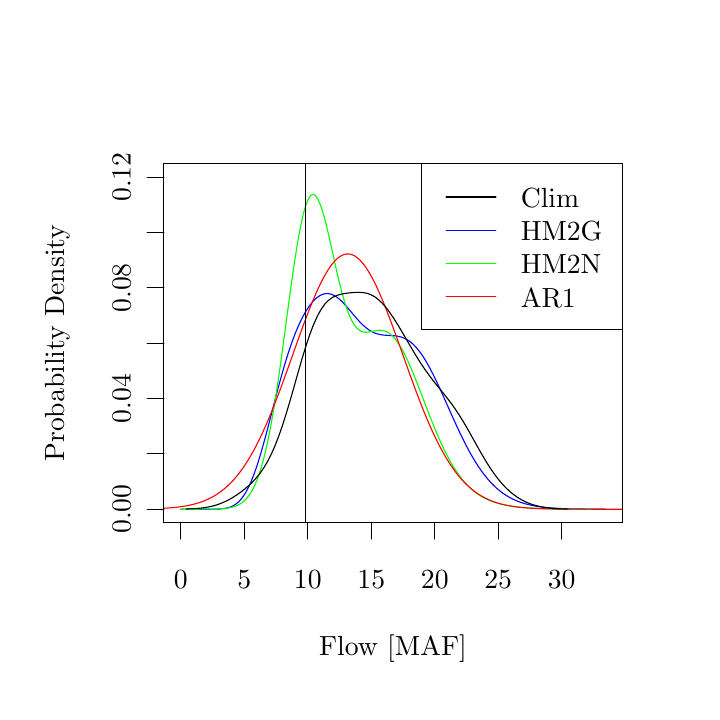
\begin{tikzpicture}[x=1pt,y=1pt]
\definecolor[named]{drawColor}{rgb}{0.00,0.00,0.00}
\definecolor[named]{fillColor}{rgb}{1.00,1.00,1.00}
\fill[color=fillColor,] (0,0) rectangle (240.00,240.00);
\begin{scope}
\path[clip] ( 49.20, 61.20) rectangle (214.80,190.80);
\definecolor[named]{drawColor}{rgb}{0.00,0.00,1.00}

\draw[color=drawColor,line cap=round,line join=round,fill opacity=0.00,] ( 55.33, 66.00) --
	( 55.64, 66.00) --
	( 55.95, 66.00) --
	( 56.26, 66.00) --
	( 56.56, 66.00) --
	( 56.87, 66.00) --
	( 57.18, 66.00) --
	( 57.48, 66.00) --
	( 57.79, 66.00) --
	( 58.10, 66.00) --
	( 58.41, 66.00) --
	( 58.71, 66.00) --
	( 59.02, 66.00) --
	( 59.33, 66.00) --
	( 59.64, 66.00) --
	( 59.94, 66.00) --
	( 60.25, 66.00) --
	( 60.56, 66.00) --
	( 60.86, 66.00) --
	( 61.17, 66.00) --
	( 61.48, 66.00) --
	( 61.79, 66.00) --
	( 62.09, 66.00) --
	( 62.40, 66.00) --
	( 62.71, 66.00) --
	( 63.02, 66.00) --
	( 63.32, 66.00) --
	( 63.63, 66.00) --
	( 63.94, 66.00) --
	( 64.24, 66.00) --
	( 64.55, 66.00) --
	( 64.86, 66.00) --
	( 65.17, 66.00) --
	( 65.47, 66.00) --
	( 65.78, 66.00) --
	( 66.09, 66.01) --
	( 66.40, 66.01) --
	( 66.70, 66.01) --
	( 67.01, 66.01) --
	( 67.32, 66.02) --
	( 67.62, 66.02) --
	( 67.93, 66.03) --
	( 68.24, 66.04) --
	( 68.55, 66.05) --
	( 68.85, 66.06) --
	( 69.16, 66.08) --
	( 69.47, 66.09) --
	( 69.78, 66.11) --
	( 70.08, 66.14) --
	( 70.39, 66.17) --
	( 70.70, 66.20) --
	( 71.00, 66.24) --
	( 71.31, 66.29) --
	( 71.62, 66.35) --
	( 71.93, 66.41) --
	( 72.23, 66.48) --
	( 72.54, 66.56) --
	( 72.85, 66.65) --
	( 73.16, 66.76) --
	( 73.46, 66.88) --
	( 73.77, 67.01) --
	( 74.08, 67.15) --
	( 74.38, 67.31) --
	( 74.69, 67.49) --
	( 75.00, 67.69) --
	( 75.31, 67.91) --
	( 75.61, 68.15) --
	( 75.92, 68.41) --
	( 76.23, 68.69) --
	( 76.54, 68.99) --
	( 76.84, 69.32) --
	( 77.15, 69.68) --
	( 77.46, 70.07) --
	( 77.76, 70.48) --
	( 78.07, 70.92) --
	( 78.38, 71.39) --
	( 78.69, 71.89) --
	( 78.99, 72.41) --
	( 79.30, 72.97) --
	( 79.61, 73.57) --
	( 79.92, 74.19) --
	( 80.22, 74.84) --
	( 80.53, 75.53) --
	( 80.84, 76.25) --
	( 81.14, 77.00) --
	( 81.45, 77.78) --
	( 81.76, 78.59) --
	( 82.07, 79.44) --
	( 82.37, 80.31) --
	( 82.68, 81.21) --
	( 82.99, 82.14) --
	( 83.30, 83.09) --
	( 83.60, 84.07) --
	( 83.91, 85.08) --
	( 84.22, 86.11) --
	( 84.53, 87.16) --
	( 84.83, 88.24) --
	( 85.14, 89.33) --
	( 85.45, 90.44) --
	( 85.75, 91.57) --
	( 86.06, 92.71) --
	( 86.37, 93.86) --
	( 86.68, 95.03) --
	( 86.98, 96.20) --
	( 87.29, 97.38) --
	( 87.60, 98.57) --
	( 87.91, 99.76) --
	( 88.21,100.95) --
	( 88.52,102.15) --
	( 88.83,103.34) --
	( 89.13,104.53) --
	( 89.44,105.72) --
	( 89.75,106.90) --
	( 90.06,108.07) --
	( 90.36,109.23) --
	( 90.67,110.38) --
	( 90.98,111.53) --
	( 91.29,112.65) --
	( 91.59,113.77) --
	( 91.90,114.87) --
	( 92.21,115.95) --
	( 92.51,117.02) --
	( 92.82,118.06) --
	( 93.13,119.09) --
	( 93.44,120.10) --
	( 93.74,121.09) --
	( 94.05,122.06) --
	( 94.36,123.01) --
	( 94.67,123.94) --
	( 94.97,124.85) --
	( 95.28,125.73) --
	( 95.59,126.60) --
	( 95.89,127.44) --
	( 96.20,128.26) --
	( 96.51,129.06) --
	( 96.82,129.83) --
	( 97.12,130.59) --
	( 97.43,131.32) --
	( 97.74,132.03) --
	( 98.05,132.72) --
	( 98.35,133.39) --
	( 98.66,134.03) --
	( 98.97,134.66) --
	( 99.27,135.26) --
	( 99.58,135.84) --
	( 99.89,136.41) --
	(100.20,136.95) --
	(100.50,137.47) --
	(100.81,137.97) --
	(101.12,138.45) --
	(101.43,138.92) --
	(101.73,139.36) --
	(102.04,139.78) --
	(102.35,140.18) --
	(102.65,140.56) --
	(102.96,140.92) --
	(103.27,141.26) --
	(103.58,141.58) --
	(103.88,141.88) --
	(104.19,142.16) --
	(104.50,142.42) --
	(104.81,142.66) --
	(105.11,142.88) --
	(105.42,143.07) --
	(105.73,143.25) --
	(106.03,143.41) --
	(106.34,143.54) --
	(106.65,143.65) --
	(106.96,143.75) --
	(107.26,143.82) --
	(107.57,143.87) --
	(107.88,143.90) --
	(108.19,143.91) --
	(108.49,143.90) --
	(108.80,143.86) --
	(109.11,143.81) --
	(109.41,143.74) --
	(109.72,143.65) --
	(110.03,143.53) --
	(110.34,143.40) --
	(110.64,143.25) --
	(110.95,143.08) --
	(111.26,142.90) --
	(111.57,142.70) --
	(111.87,142.48) --
	(112.18,142.24) --
	(112.49,141.99) --
	(112.79,141.73) --
	(113.10,141.45) --
	(113.41,141.16) --
	(113.72,140.86) --
	(114.02,140.54) --
	(114.33,140.22) --
	(114.64,139.89) --
	(114.95,139.55) --
	(115.25,139.20) --
	(115.56,138.85) --
	(115.87,138.49) --
	(116.18,138.13) --
	(116.48,137.76) --
	(116.79,137.40) --
	(117.10,137.03) --
	(117.40,136.66) --
	(117.71,136.30) --
	(118.02,135.93) --
	(118.33,135.57) --
	(118.63,135.22) --
	(118.94,134.86) --
	(119.25,134.52) --
	(119.56,134.18) --
	(119.86,133.85) --
	(120.17,133.52) --
	(120.48,133.21) --
	(120.78,132.90) --
	(121.09,132.60) --
	(121.40,132.32) --
	(121.71,132.04) --
	(122.01,131.78) --
	(122.32,131.53) --
	(122.63,131.29) --
	(122.94,131.06) --
	(123.24,130.85) --
	(123.55,130.64) --
	(123.86,130.45) --
	(124.16,130.28) --
	(124.47,130.11) --
	(124.78,129.96) --
	(125.09,129.81) --
	(125.39,129.68) --
	(125.70,129.57) --
	(126.01,129.46) --
	(126.32,129.36) --
	(126.62,129.28) --
	(126.93,129.20) --
	(127.24,129.13) --
	(127.54,129.07) --
	(127.85,129.02) --
	(128.16,128.98) --
	(128.47,128.94) --
	(128.77,128.91) --
	(129.08,128.88) --
	(129.39,128.85) --
	(129.70,128.84) --
	(130.00,128.82) --
	(130.31,128.80) --
	(130.62,128.79) --
	(130.92,128.77) --
	(131.23,128.76) --
	(131.54,128.74) --
	(131.85,128.72) --
	(132.15,128.70) --
	(132.46,128.67) --
	(132.77,128.64) --
	(133.08,128.61) --
	(133.38,128.56) --
	(133.69,128.51) --
	(134.00,128.45) --
	(134.30,128.39) --
	(134.61,128.31) --
	(134.92,128.22) --
	(135.23,128.12) --
	(135.53,128.01) --
	(135.84,127.89) --
	(136.15,127.76) --
	(136.46,127.61) --
	(136.76,127.45) --
	(137.07,127.28) --
	(137.38,127.09) --
	(137.68,126.89) --
	(137.99,126.67) --
	(138.30,126.44) --
	(138.61,126.20) --
	(138.91,125.93) --
	(139.22,125.65) --
	(139.53,125.36) --
	(139.84,125.05) --
	(140.14,124.72) --
	(140.45,124.38) --
	(140.76,124.02) --
	(141.06,123.65) --
	(141.37,123.26) --
	(141.68,122.86) --
	(141.99,122.44) --
	(142.29,122.00) --
	(142.60,121.55) --
	(142.91,121.09) --
	(143.22,120.61) --
	(143.52,120.11) --
	(143.83,119.61) --
	(144.14,119.09) --
	(144.44,118.55) --
	(144.75,118.01) --
	(145.06,117.45) --
	(145.37,116.88) --
	(145.67,116.30) --
	(145.98,115.71) --
	(146.29,115.11) --
	(146.60,114.50) --
	(146.90,113.88) --
	(147.21,113.25) --
	(147.52,112.61) --
	(147.82,111.97) --
	(148.13,111.32) --
	(148.44,110.66) --
	(148.75,110.00) --
	(149.05,109.33) --
	(149.36,108.66) --
	(149.67,107.98) --
	(149.98,107.30) --
	(150.28,106.62) --
	(150.59,105.93) --
	(150.90,105.24) --
	(151.21,104.55) --
	(151.51,103.86) --
	(151.82,103.17) --
	(152.13,102.48) --
	(152.43,101.79) --
	(152.74,101.10) --
	(153.05,100.41) --
	(153.36, 99.73) --
	(153.66, 99.05) --
	(153.97, 98.37) --
	(154.28, 97.69) --
	(154.59, 97.02) --
	(154.89, 96.35) --
	(155.20, 95.68) --
	(155.51, 95.03) --
	(155.81, 94.37) --
	(156.12, 93.73) --
	(156.43, 93.08) --
	(156.74, 92.45) --
	(157.04, 91.82) --
	(157.35, 91.20) --
	(157.66, 90.58) --
	(157.97, 89.98) --
	(158.27, 89.38) --
	(158.58, 88.78) --
	(158.89, 88.20) --
	(159.19, 87.62) --
	(159.50, 87.06) --
	(159.81, 86.50) --
	(160.12, 85.95) --
	(160.42, 85.41) --
	(160.73, 84.88) --
	(161.04, 84.35) --
	(161.35, 83.84) --
	(161.65, 83.33) --
	(161.96, 82.84) --
	(162.27, 82.35) --
	(162.57, 81.87) --
	(162.88, 81.41) --
	(163.19, 80.95) --
	(163.50, 80.50) --
	(163.80, 80.06) --
	(164.11, 79.63) --
	(164.42, 79.21) --
	(164.73, 78.80) --
	(165.03, 78.40) --
	(165.34, 78.00) --
	(165.65, 77.62) --
	(165.95, 77.25) --
	(166.26, 76.88) --
	(166.57, 76.52) --
	(166.88, 76.18) --
	(167.18, 75.84) --
	(167.49, 75.51) --
	(167.80, 75.19) --
	(168.11, 74.87) --
	(168.41, 74.57) --
	(168.72, 74.27) --
	(169.03, 73.98) --
	(169.33, 73.70) --
	(169.64, 73.43) --
	(169.95, 73.17) --
	(170.26, 72.91) --
	(170.56, 72.66) --
	(170.87, 72.42) --
	(171.18, 72.18) --
	(171.49, 71.96) --
	(171.79, 71.73) --
	(172.10, 71.52) --
	(172.41, 71.31) --
	(172.71, 71.11) --
	(173.02, 70.92) --
	(173.33, 70.73) --
	(173.64, 70.55) --
	(173.94, 70.37) --
	(174.25, 70.20) --
	(174.56, 70.04) --
	(174.87, 69.88) --
	(175.17, 69.72) --
	(175.48, 69.57) --
	(175.79, 69.43) --
	(176.09, 69.29) --
	(176.40, 69.16) --
	(176.71, 69.03) --
	(177.02, 68.90) --
	(177.32, 68.78) --
	(177.63, 68.67) --
	(177.94, 68.56) --
	(178.25, 68.45) --
	(178.55, 68.35) --
	(178.86, 68.25) --
	(179.17, 68.15) --
	(179.47, 68.06) --
	(179.78, 67.97) --
	(180.09, 67.89) --
	(180.40, 67.80) --
	(180.70, 67.73) --
	(181.01, 67.65) --
	(181.32, 67.58) --
	(181.63, 67.51) --
	(181.93, 67.44) --
	(182.24, 67.38) --
	(182.55, 67.31) --
	(182.86, 67.25) --
	(183.16, 67.20) --
	(183.47, 67.14) --
	(183.78, 67.09) --
	(184.08, 67.04) --
	(184.39, 66.99) --
	(184.70, 66.95) --
	(185.01, 66.90) --
	(185.31, 66.86) --
	(185.62, 66.82) --
	(185.93, 66.78) --
	(186.24, 66.75) --
	(186.54, 66.71) --
	(186.85, 66.68) --
	(187.16, 66.64) --
	(187.46, 66.61) --
	(187.77, 66.58) --
	(188.08, 66.55) --
	(188.39, 66.53) --
	(188.69, 66.50) --
	(189.00, 66.48) --
	(189.31, 66.45) --
	(189.62, 66.43) --
	(189.92, 66.41) --
	(190.23, 66.39) --
	(190.54, 66.37) --
	(190.84, 66.35) --
	(191.15, 66.33) --
	(191.46, 66.32) --
	(191.77, 66.30) --
	(192.07, 66.29) --
	(192.38, 66.27) --
	(192.69, 66.26) --
	(193.00, 66.24) --
	(193.30, 66.23) --
	(193.61, 66.22) --
	(193.92, 66.21) --
	(194.22, 66.20) --
	(194.53, 66.19) --
	(194.84, 66.18) --
	(195.15, 66.17) --
	(195.45, 66.16) --
	(195.76, 66.15) --
	(196.07, 66.14) --
	(196.38, 66.14) --
	(196.68, 66.13) --
	(196.99, 66.12) --
	(197.30, 66.11) --
	(197.60, 66.11) --
	(197.91, 66.10) --
	(198.22, 66.10) --
	(198.53, 66.09) --
	(198.83, 66.09) --
	(199.14, 66.08) --
	(199.45, 66.08) --
	(199.76, 66.07) --
	(200.06, 66.07) --
	(200.37, 66.07) --
	(200.68, 66.06) --
	(200.98, 66.06) --
	(201.29, 66.06) --
	(201.60, 66.05) --
	(201.91, 66.05) --
	(202.21, 66.05) --
	(202.52, 66.04) --
	(202.83, 66.04) --
	(203.14, 66.04) --
	(203.44, 66.04) --
	(203.75, 66.03) --
	(204.06, 66.03) --
	(204.36, 66.03) --
	(204.67, 66.03) --
	(204.98, 66.03) --
	(205.29, 66.03) --
	(205.59, 66.02) --
	(205.90, 66.02) --
	(206.21, 66.02) --
	(206.52, 66.02) --
	(206.82, 66.02) --
	(207.13, 66.02) --
	(207.44, 66.02) --
	(207.74, 66.02) --
	(208.05, 66.02) --
	(208.36, 66.01) --
	(208.67, 66.01);
\end{scope}
\begin{scope}
\path[clip] (  0.00,  0.00) rectangle (240.00,240.00);
\definecolor[named]{drawColor}{rgb}{0.00,0.00,0.00}

\draw[color=drawColor,line cap=round,line join=round,fill opacity=0.00,] ( 55.33, 61.20) -- (192.98, 61.20);

\draw[color=drawColor,line cap=round,line join=round,fill opacity=0.00,] ( 55.33, 61.20) -- ( 55.33, 55.20);

\draw[color=drawColor,line cap=round,line join=round,fill opacity=0.00,] ( 78.27, 61.20) -- ( 78.27, 55.20);

\draw[color=drawColor,line cap=round,line join=round,fill opacity=0.00,] (101.22, 61.20) -- (101.22, 55.20);

\draw[color=drawColor,line cap=round,line join=round,fill opacity=0.00,] (124.16, 61.20) -- (124.16, 55.20);

\draw[color=drawColor,line cap=round,line join=round,fill opacity=0.00,] (147.10, 61.20) -- (147.10, 55.20);

\draw[color=drawColor,line cap=round,line join=round,fill opacity=0.00,] (170.04, 61.20) -- (170.04, 55.20);

\draw[color=drawColor,line cap=round,line join=round,fill opacity=0.00,] (192.98, 61.20) -- (192.98, 55.20);

\node[color=drawColor,anchor=base,inner sep=0pt, outer sep=0pt, scale=  1.00] at ( 55.33, 37.20) {0%
};

\node[color=drawColor,anchor=base,inner sep=0pt, outer sep=0pt, scale=  1.00] at ( 78.27, 37.20) {5%
};

\node[color=drawColor,anchor=base,inner sep=0pt, outer sep=0pt, scale=  1.00] at (101.22, 37.20) {10%
};

\node[color=drawColor,anchor=base,inner sep=0pt, outer sep=0pt, scale=  1.00] at (124.16, 37.20) {15%
};

\node[color=drawColor,anchor=base,inner sep=0pt, outer sep=0pt, scale=  1.00] at (147.10, 37.20) {20%
};

\node[color=drawColor,anchor=base,inner sep=0pt, outer sep=0pt, scale=  1.00] at (170.04, 37.20) {25%
};

\node[color=drawColor,anchor=base,inner sep=0pt, outer sep=0pt, scale=  1.00] at (192.98, 37.20) {30%
};

\draw[color=drawColor,line cap=round,line join=round,fill opacity=0.00,] ( 49.20, 66.00) -- ( 49.20,186.00);

\draw[color=drawColor,line cap=round,line join=round,fill opacity=0.00,] ( 49.20, 66.00) -- ( 43.20, 66.00);

\draw[color=drawColor,line cap=round,line join=round,fill opacity=0.00,] ( 49.20, 86.00) -- ( 43.20, 86.00);

\draw[color=drawColor,line cap=round,line join=round,fill opacity=0.00,] ( 49.20,106.00) -- ( 43.20,106.00);

\draw[color=drawColor,line cap=round,line join=round,fill opacity=0.00,] ( 49.20,126.00) -- ( 43.20,126.00);

\draw[color=drawColor,line cap=round,line join=round,fill opacity=0.00,] ( 49.20,146.00) -- ( 43.20,146.00);

\draw[color=drawColor,line cap=round,line join=round,fill opacity=0.00,] ( 49.20,166.00) -- ( 43.20,166.00);

\draw[color=drawColor,line cap=round,line join=round,fill opacity=0.00,] ( 49.20,186.00) -- ( 43.20,186.00);

\node[rotate= 90.00,color=drawColor,anchor=base,inner sep=0pt, outer sep=0pt, scale=  1.00] at ( 37.20, 66.00) {0.00%
};

\node[rotate= 90.00,color=drawColor,anchor=base,inner sep=0pt, outer sep=0pt, scale=  1.00] at ( 37.20,106.00) {0.04%
};

\node[rotate= 90.00,color=drawColor,anchor=base,inner sep=0pt, outer sep=0pt, scale=  1.00] at ( 37.20,146.00) {0.08%
};

\node[rotate= 90.00,color=drawColor,anchor=base,inner sep=0pt, outer sep=0pt, scale=  1.00] at ( 37.20,186.00) {0.12%
};

\draw[color=drawColor,line cap=round,line join=round,fill opacity=0.00,] ( 49.20, 61.20) --
	(214.80, 61.20) --
	(214.80,190.80) --
	( 49.20,190.80) --
	( 49.20, 61.20);
\end{scope}
\begin{scope}
\path[clip] (  0.00,  0.00) rectangle (240.00,240.00);
\definecolor[named]{drawColor}{rgb}{0.00,0.00,0.00}

\node[color=drawColor,anchor=base,inner sep=0pt, outer sep=0pt, scale=  1.00] at (132.00, 13.20) {Flow [MAF]%
};

\node[rotate= 90.00,color=drawColor,anchor=base,inner sep=0pt, outer sep=0pt, scale=  1.00] at ( 13.20,126.00) {Probability Density%
};
\end{scope}
\begin{scope}
\path[clip] ( 49.20, 61.20) rectangle (214.80,190.80);
\definecolor[named]{drawColor}{rgb}{0.00,1.00,0.00}

\draw[color=drawColor,line cap=round,line join=round,fill opacity=0.00,] ( 55.33, 66.00) --
	( 55.64, 66.00) --
	( 55.95, 66.00) --
	( 56.26, 66.00) --
	( 56.56, 66.00) --
	( 56.87, 66.00) --
	( 57.18, 66.00) --
	( 57.48, 66.00) --
	( 57.79, 66.00) --
	( 58.10, 66.00) --
	( 58.41, 66.00) --
	( 58.71, 66.00) --
	( 59.02, 66.00) --
	( 59.33, 66.00) --
	( 59.64, 66.00) --
	( 59.94, 66.00) --
	( 60.25, 66.00) --
	( 60.56, 66.00) --
	( 60.86, 66.00) --
	( 61.17, 66.00) --
	( 61.48, 66.00) --
	( 61.79, 66.00) --
	( 62.09, 66.01) --
	( 62.40, 66.01) --
	( 62.71, 66.01) --
	( 63.02, 66.01) --
	( 63.32, 66.01) --
	( 63.63, 66.01) --
	( 63.94, 66.01) --
	( 64.24, 66.01) --
	( 64.55, 66.02) --
	( 64.86, 66.02) --
	( 65.17, 66.02) --
	( 65.47, 66.03) --
	( 65.78, 66.03) --
	( 66.09, 66.03) --
	( 66.40, 66.04) --
	( 66.70, 66.04) --
	( 67.01, 66.05) --
	( 67.32, 66.06) --
	( 67.62, 66.06) --
	( 67.93, 66.07) --
	( 68.24, 66.08) --
	( 68.55, 66.09) --
	( 68.85, 66.11) --
	( 69.16, 66.12) --
	( 69.47, 66.14) --
	( 69.78, 66.16) --
	( 70.08, 66.18) --
	( 70.39, 66.20) --
	( 70.70, 66.22) --
	( 71.00, 66.25) --
	( 71.31, 66.28) --
	( 71.62, 66.32) --
	( 71.93, 66.36) --
	( 72.23, 66.40) --
	( 72.54, 66.45) --
	( 72.85, 66.51) --
	( 73.16, 66.56) --
	( 73.46, 66.63) --
	( 73.77, 66.70) --
	( 74.08, 66.78) --
	( 74.38, 66.87) --
	( 74.69, 66.97) --
	( 75.00, 67.08) --
	( 75.31, 67.19) --
	( 75.61, 67.32) --
	( 75.92, 67.46) --
	( 76.23, 67.62) --
	( 76.54, 67.79) --
	( 76.84, 67.97) --
	( 77.15, 68.17) --
	( 77.46, 68.39) --
	( 77.76, 68.62) --
	( 78.07, 68.88) --
	( 78.38, 69.16) --
	( 78.69, 69.46) --
	( 78.99, 69.78) --
	( 79.30, 70.13) --
	( 79.61, 70.50) --
	( 79.92, 70.91) --
	( 80.22, 71.34) --
	( 80.53, 71.81) --
	( 80.84, 72.31) --
	( 81.14, 72.85) --
	( 81.45, 73.42) --
	( 81.76, 74.03) --
	( 82.07, 74.68) --
	( 82.37, 75.37) --
	( 82.68, 76.11) --
	( 82.99, 76.89) --
	( 83.30, 77.71) --
	( 83.60, 78.59) --
	( 83.91, 79.51) --
	( 84.22, 80.48) --
	( 84.53, 81.51) --
	( 84.83, 82.59) --
	( 85.14, 83.72) --
	( 85.45, 84.91) --
	( 85.75, 86.15) --
	( 86.06, 87.46) --
	( 86.37, 88.81) --
	( 86.68, 90.23) --
	( 86.98, 91.70) --
	( 87.29, 93.23) --
	( 87.60, 94.82) --
	( 87.91, 96.47) --
	( 88.21, 98.17) --
	( 88.52, 99.93) --
	( 88.83,101.74) --
	( 89.13,103.60) --
	( 89.44,105.51) --
	( 89.75,107.47) --
	( 90.06,109.48) --
	( 90.36,111.54) --
	( 90.67,113.63) --
	( 90.98,115.76) --
	( 91.29,117.93) --
	( 91.59,120.13) --
	( 91.90,122.36) --
	( 92.21,124.61) --
	( 92.51,126.88) --
	( 92.82,129.16) --
	( 93.13,131.46) --
	( 93.44,133.75) --
	( 93.74,136.05) --
	( 94.05,138.35) --
	( 94.36,140.63) --
	( 94.67,142.90) --
	( 94.97,145.14) --
	( 95.28,147.36) --
	( 95.59,149.55) --
	( 95.89,151.70) --
	( 96.20,153.80) --
	( 96.51,155.85) --
	( 96.82,157.85) --
	( 97.12,159.79) --
	( 97.43,161.66) --
	( 97.74,163.46) --
	( 98.05,165.19) --
	( 98.35,166.84) --
	( 98.66,168.40) --
	( 98.97,169.87) --
	( 99.27,171.25) --
	( 99.58,172.53) --
	( 99.89,173.72) --
	(100.20,174.80) --
	(100.50,175.78) --
	(100.81,176.65) --
	(101.12,177.41) --
	(101.43,178.06) --
	(101.73,178.61) --
	(102.04,179.04) --
	(102.35,179.36) --
	(102.65,179.58) --
	(102.96,179.68) --
	(103.27,179.68) --
	(103.58,179.57) --
	(103.88,179.35) --
	(104.19,179.04) --
	(104.50,178.63) --
	(104.81,178.12) --
	(105.11,177.52) --
	(105.42,176.83) --
	(105.73,176.06) --
	(106.03,175.22) --
	(106.34,174.29) --
	(106.65,173.30) --
	(106.96,172.25) --
	(107.26,171.14) --
	(107.57,169.97) --
	(107.88,168.76) --
	(108.19,167.50) --
	(108.49,166.21) --
	(108.80,164.89) --
	(109.11,163.54) --
	(109.41,162.17) --
	(109.72,160.79) --
	(110.03,159.40) --
	(110.34,158.00) --
	(110.64,156.61) --
	(110.95,155.23) --
	(111.26,153.85) --
	(111.57,152.49) --
	(111.87,151.15) --
	(112.18,149.83) --
	(112.49,148.54) --
	(112.79,147.29) --
	(113.10,146.06) --
	(113.41,144.87) --
	(113.72,143.73) --
	(114.02,142.62) --
	(114.33,141.56) --
	(114.64,140.55) --
	(114.95,139.58) --
	(115.25,138.66) --
	(115.56,137.79) --
	(115.87,136.97) --
	(116.18,136.20) --
	(116.48,135.48) --
	(116.79,134.81) --
	(117.10,134.19) --
	(117.40,133.61) --
	(117.71,133.09) --
	(118.02,132.62) --
	(118.33,132.19) --
	(118.63,131.80) --
	(118.94,131.46) --
	(119.25,131.16) --
	(119.56,130.89) --
	(119.86,130.67) --
	(120.17,130.48) --
	(120.48,130.32) --
	(120.78,130.20) --
	(121.09,130.10) --
	(121.40,130.03) --
	(121.71,129.98) --
	(122.01,129.96) --
	(122.32,129.95) --
	(122.63,129.96) --
	(122.94,129.99) --
	(123.24,130.03) --
	(123.55,130.08) --
	(123.86,130.13) --
	(124.16,130.19) --
	(124.47,130.26) --
	(124.78,130.32) --
	(125.09,130.39) --
	(125.39,130.45) --
	(125.70,130.50) --
	(126.01,130.55) --
	(126.32,130.60) --
	(126.62,130.63) --
	(126.93,130.65) --
	(127.24,130.66) --
	(127.54,130.65) --
	(127.85,130.63) --
	(128.16,130.59) --
	(128.47,130.54) --
	(128.77,130.46) --
	(129.08,130.37) --
	(129.39,130.26) --
	(129.70,130.12) --
	(130.00,129.97) --
	(130.31,129.79) --
	(130.62,129.59) --
	(130.92,129.37) --
	(131.23,129.12) --
	(131.54,128.85) --
	(131.85,128.56) --
	(132.15,128.24) --
	(132.46,127.90) --
	(132.77,127.54) --
	(133.08,127.15) --
	(133.38,126.75) --
	(133.69,126.31) --
	(134.00,125.86) --
	(134.30,125.39) --
	(134.61,124.89) --
	(134.92,124.37) --
	(135.23,123.83) --
	(135.53,123.28) --
	(135.84,122.70) --
	(136.15,122.10) --
	(136.46,121.49) --
	(136.76,120.86) --
	(137.07,120.21) --
	(137.38,119.55) --
	(137.68,118.87) --
	(137.99,118.18) --
	(138.30,117.48) --
	(138.61,116.76) --
	(138.91,116.03) --
	(139.22,115.29) --
	(139.53,114.54) --
	(139.84,113.78) --
	(140.14,113.02) --
	(140.45,112.24) --
	(140.76,111.46) --
	(141.06,110.67) --
	(141.37,109.88) --
	(141.68,109.09) --
	(141.99,108.29) --
	(142.29,107.49) --
	(142.60,106.68) --
	(142.91,105.88) --
	(143.22,105.07) --
	(143.52,104.27) --
	(143.83,103.47) --
	(144.14,102.67) --
	(144.44,101.87) --
	(144.75,101.07) --
	(145.06,100.28) --
	(145.37, 99.50) --
	(145.67, 98.72) --
	(145.98, 97.94) --
	(146.29, 97.17) --
	(146.60, 96.41) --
	(146.90, 95.66) --
	(147.21, 94.91) --
	(147.52, 94.18) --
	(147.82, 93.45) --
	(148.13, 92.73) --
	(148.44, 92.02) --
	(148.75, 91.31) --
	(149.05, 90.62) --
	(149.36, 89.94) --
	(149.67, 89.27) --
	(149.98, 88.62) --
	(150.28, 87.97) --
	(150.59, 87.33) --
	(150.90, 86.71) --
	(151.21, 86.10) --
	(151.51, 85.50) --
	(151.82, 84.91) --
	(152.13, 84.33) --
	(152.43, 83.77) --
	(152.74, 83.21) --
	(153.05, 82.67) --
	(153.36, 82.15) --
	(153.66, 81.63) --
	(153.97, 81.13) --
	(154.28, 80.63) --
	(154.59, 80.16) --
	(154.89, 79.69) --
	(155.20, 79.23) --
	(155.51, 78.79) --
	(155.81, 78.36) --
	(156.12, 77.94) --
	(156.43, 77.53) --
	(156.74, 77.13) --
	(157.04, 76.75) --
	(157.35, 76.37) --
	(157.66, 76.01) --
	(157.97, 75.65) --
	(158.27, 75.31) --
	(158.58, 74.98) --
	(158.89, 74.66) --
	(159.19, 74.35) --
	(159.50, 74.04) --
	(159.81, 73.75) --
	(160.12, 73.47) --
	(160.42, 73.19) --
	(160.73, 72.93) --
	(161.04, 72.67) --
	(161.35, 72.42) --
	(161.65, 72.18) --
	(161.96, 71.95) --
	(162.27, 71.73) --
	(162.57, 71.51) --
	(162.88, 71.30) --
	(163.19, 71.10) --
	(163.50, 70.91) --
	(163.80, 70.72) --
	(164.11, 70.54) --
	(164.42, 70.37) --
	(164.73, 70.20) --
	(165.03, 70.04) --
	(165.34, 69.88) --
	(165.65, 69.73) --
	(165.95, 69.58) --
	(166.26, 69.45) --
	(166.57, 69.31) --
	(166.88, 69.18) --
	(167.18, 69.06) --
	(167.49, 68.94) --
	(167.80, 68.82) --
	(168.11, 68.71) --
	(168.41, 68.60) --
	(168.72, 68.50) --
	(169.03, 68.40) --
	(169.33, 68.31) --
	(169.64, 68.22) --
	(169.95, 68.13) --
	(170.26, 68.04) --
	(170.56, 67.96) --
	(170.87, 67.88) --
	(171.18, 67.81) --
	(171.49, 67.74) --
	(171.79, 67.67) --
	(172.10, 67.60) --
	(172.41, 67.54) --
	(172.71, 67.47) --
	(173.02, 67.41) --
	(173.33, 67.36) --
	(173.64, 67.30) --
	(173.94, 67.25) --
	(174.25, 67.20) --
	(174.56, 67.15) --
	(174.87, 67.10) --
	(175.17, 67.06) --
	(175.48, 67.02) --
	(175.79, 66.97) --
	(176.09, 66.93) --
	(176.40, 66.90) --
	(176.71, 66.86) --
	(177.02, 66.82) --
	(177.32, 66.79) --
	(177.63, 66.76) --
	(177.94, 66.72) --
	(178.25, 66.69) --
	(178.55, 66.66) --
	(178.86, 66.64) --
	(179.17, 66.61) --
	(179.47, 66.58) --
	(179.78, 66.56) --
	(180.09, 66.54) --
	(180.40, 66.51) --
	(180.70, 66.49) --
	(181.01, 66.47) --
	(181.32, 66.45) --
	(181.63, 66.43) --
	(181.93, 66.41) --
	(182.24, 66.39) --
	(182.55, 66.38) --
	(182.86, 66.36) --
	(183.16, 66.34) --
	(183.47, 66.33) --
	(183.78, 66.31) --
	(184.08, 66.30) --
	(184.39, 66.29) --
	(184.70, 66.27) --
	(185.01, 66.26) --
	(185.31, 66.25) --
	(185.62, 66.24) --
	(185.93, 66.23) --
	(186.24, 66.22) --
	(186.54, 66.21) --
	(186.85, 66.20) --
	(187.16, 66.19) --
	(187.46, 66.18) --
	(187.77, 66.17) --
	(188.08, 66.16) --
	(188.39, 66.15) --
	(188.69, 66.15) --
	(189.00, 66.14) --
	(189.31, 66.13) --
	(189.62, 66.13) --
	(189.92, 66.12) --
	(190.23, 66.11) --
	(190.54, 66.11) --
	(190.84, 66.10) --
	(191.15, 66.10) --
	(191.46, 66.09) --
	(191.77, 66.09) --
	(192.07, 66.08) --
	(192.38, 66.08) --
	(192.69, 66.08) --
	(193.00, 66.07) --
	(193.30, 66.07) --
	(193.61, 66.06) --
	(193.92, 66.06) --
	(194.22, 66.06) --
	(194.53, 66.06) --
	(194.84, 66.05) --
	(195.15, 66.05) --
	(195.45, 66.05) --
	(195.76, 66.04) --
	(196.07, 66.04) --
	(196.38, 66.04) --
	(196.68, 66.04) --
	(196.99, 66.04) --
	(197.30, 66.03) --
	(197.60, 66.03) --
	(197.91, 66.03) --
	(198.22, 66.03) --
	(198.53, 66.03) --
	(198.83, 66.03) --
	(199.14, 66.02) --
	(199.45, 66.02) --
	(199.76, 66.02) --
	(200.06, 66.02) --
	(200.37, 66.02) --
	(200.68, 66.02) --
	(200.98, 66.02) --
	(201.29, 66.02) --
	(201.60, 66.01) --
	(201.91, 66.01) --
	(202.21, 66.01) --
	(202.52, 66.01) --
	(202.83, 66.01) --
	(203.14, 66.01) --
	(203.44, 66.01) --
	(203.75, 66.01) --
	(204.06, 66.01) --
	(204.36, 66.01) --
	(204.67, 66.01) --
	(204.98, 66.01) --
	(205.29, 66.01) --
	(205.59, 66.01) --
	(205.90, 66.01) --
	(206.21, 66.01) --
	(206.52, 66.01) --
	(206.82, 66.01) --
	(207.13, 66.00) --
	(207.44, 66.00) --
	(207.74, 66.00) --
	(208.05, 66.00) --
	(208.36, 66.00) --
	(208.67, 66.00);
\definecolor[named]{drawColor}{rgb}{1.00,0.00,0.00}

\draw[color=drawColor,line cap=round,line join=round,fill opacity=0.00,] ( 34.46, 66.02) --
	( 34.83, 66.02) --
	( 35.20, 66.02) --
	( 35.57, 66.03) --
	( 35.93, 66.03) --
	( 36.30, 66.03) --
	( 36.67, 66.03) --
	( 37.04, 66.04) --
	( 37.40, 66.04) --
	( 37.77, 66.04) --
	( 38.14, 66.04) --
	( 38.51, 66.05) --
	( 38.87, 66.05) --
	( 39.24, 66.06) --
	( 39.61, 66.06) --
	( 39.97, 66.06) --
	( 40.34, 66.07) --
	( 40.71, 66.07) --
	( 41.08, 66.08) --
	( 41.44, 66.08) --
	( 41.81, 66.09) --
	( 42.18, 66.10) --
	( 42.55, 66.10) --
	( 42.91, 66.11) --
	( 43.28, 66.12) --
	( 43.65, 66.13) --
	( 44.02, 66.14) --
	( 44.38, 66.15) --
	( 44.75, 66.16) --
	( 45.12, 66.17) --
	( 45.49, 66.18) --
	( 45.85, 66.19) --
	( 46.22, 66.20) --
	( 46.59, 66.22) --
	( 46.96, 66.23) --
	( 47.32, 66.25) --
	( 47.69, 66.26) --
	( 48.06, 66.28) --
	( 48.43, 66.30) --
	( 48.79, 66.32) --
	( 49.16, 66.34) --
	( 49.53, 66.36) --
	( 49.90, 66.38) --
	( 50.26, 66.40) --
	( 50.63, 66.43) --
	( 51.00, 66.46) --
	( 51.37, 66.48) --
	( 51.73, 66.51) --
	( 52.10, 66.55) --
	( 52.47, 66.58) --
	( 52.84, 66.61) --
	( 53.20, 66.65) --
	( 53.57, 66.69) --
	( 53.94, 66.73) --
	( 54.31, 66.77) --
	( 54.67, 66.82) --
	( 55.04, 66.87) --
	( 55.41, 66.92) --
	( 55.78, 66.97) --
	( 56.14, 67.03) --
	( 56.51, 67.08) --
	( 56.88, 67.15) --
	( 57.25, 67.21) --
	( 57.61, 67.28) --
	( 57.98, 67.35) --
	( 58.35, 67.42) --
	( 58.72, 67.50) --
	( 59.08, 67.58) --
	( 59.45, 67.67) --
	( 59.82, 67.76) --
	( 60.19, 67.85) --
	( 60.55, 67.95) --
	( 60.92, 68.05) --
	( 61.29, 68.16) --
	( 61.66, 68.27) --
	( 62.02, 68.39) --
	( 62.39, 68.51) --
	( 62.76, 68.64) --
	( 63.13, 68.77) --
	( 63.49, 68.91) --
	( 63.86, 69.05) --
	( 64.23, 69.20) --
	( 64.60, 69.36) --
	( 64.96, 69.52) --
	( 65.33, 69.69) --
	( 65.70, 69.87) --
	( 66.07, 70.06) --
	( 66.43, 70.25) --
	( 66.80, 70.45) --
	( 67.17, 70.65) --
	( 67.54, 70.87) --
	( 67.90, 71.09) --
	( 68.27, 71.32) --
	( 68.64, 71.56) --
	( 69.01, 71.81) --
	( 69.37, 72.07) --
	( 69.74, 72.33) --
	( 70.11, 72.61) --
	( 70.48, 72.90) --
	( 70.84, 73.19) --
	( 71.21, 73.50) --
	( 71.58, 73.81) --
	( 71.95, 74.14) --
	( 72.31, 74.48) --
	( 72.68, 74.83) --
	( 73.05, 75.19) --
	( 73.42, 75.56) --
	( 73.78, 75.94) --
	( 74.15, 76.33) --
	( 74.52, 76.74) --
	( 74.89, 77.16) --
	( 75.25, 77.59) --
	( 75.62, 78.03) --
	( 75.99, 78.49) --
	( 76.36, 78.96) --
	( 76.72, 79.44) --
	( 77.09, 79.93) --
	( 77.46, 80.44) --
	( 77.83, 80.96) --
	( 78.19, 81.50) --
	( 78.56, 82.05) --
	( 78.93, 82.61) --
	( 79.30, 83.19) --
	( 79.66, 83.78) --
	( 80.03, 84.38) --
	( 80.40, 85.00) --
	( 80.77, 85.63) --
	( 81.13, 86.28) --
	( 81.50, 86.94) --
	( 81.87, 87.61) --
	( 82.24, 88.30) --
	( 82.60, 89.01) --
	( 82.97, 89.72) --
	( 83.34, 90.45) --
	( 83.71, 91.20) --
	( 84.07, 91.96) --
	( 84.44, 92.73) --
	( 84.81, 93.51) --
	( 85.17, 94.31) --
	( 85.54, 95.13) --
	( 85.91, 95.95) --
	( 86.28, 96.79) --
	( 86.64, 97.64) --
	( 87.01, 98.50) --
	( 87.38, 99.38) --
	( 87.75,100.27) --
	( 88.11,101.16) --
	( 88.48,102.07) --
	( 88.85,102.99) --
	( 89.22,103.93) --
	( 89.58,104.87) --
	( 89.95,105.82) --
	( 90.32,106.78) --
	( 90.69,107.75) --
	( 91.05,108.72) --
	( 91.42,109.71) --
	( 91.79,110.70) --
	( 92.16,111.70) --
	( 92.52,112.71) --
	( 92.89,113.72) --
	( 93.26,114.74) --
	( 93.63,115.76) --
	( 93.99,116.78) --
	( 94.36,117.81) --
	( 94.73,118.84) --
	( 95.10,119.88) --
	( 95.46,120.91) --
	( 95.83,121.95) --
	( 96.20,122.98) --
	( 96.57,124.02) --
	( 96.93,125.05) --
	( 97.30,126.08) --
	( 97.67,127.11) --
	( 98.04,128.13) --
	( 98.40,129.15) --
	( 98.77,130.17) --
	( 99.14,131.18) --
	( 99.51,132.18) --
	( 99.87,133.17) --
	(100.24,134.16) --
	(100.61,135.14) --
	(100.98,136.10) --
	(101.34,137.06) --
	(101.71,138.00) --
	(102.08,138.94) --
	(102.45,139.85) --
	(102.81,140.76) --
	(103.18,141.65) --
	(103.55,142.52) --
	(103.92,143.38) --
	(104.28,144.22) --
	(104.65,145.04) --
	(105.02,145.85) --
	(105.39,146.63) --
	(105.75,147.39) --
	(106.12,148.14) --
	(106.49,148.86) --
	(106.86,149.56) --
	(107.22,150.23) --
	(107.59,150.88) --
	(107.96,151.51) --
	(108.33,152.12) --
	(108.69,152.69) --
	(109.06,153.24) --
	(109.43,153.77) --
	(109.80,154.27) --
	(110.16,154.74) --
	(110.53,155.18) --
	(110.90,155.59) --
	(111.27,155.98) --
	(111.63,156.33) --
	(112.00,156.66) --
	(112.37,156.96) --
	(112.74,157.22) --
	(113.10,157.46) --
	(113.47,157.66) --
	(113.84,157.83) --
	(114.21,157.98) --
	(114.57,158.09) --
	(114.94,158.16) --
	(115.31,158.21) --
	(115.68,158.23) --
	(116.04,158.21) --
	(116.41,158.16) --
	(116.78,158.09) --
	(117.15,157.98) --
	(117.51,157.83) --
	(117.88,157.66) --
	(118.25,157.46) --
	(118.62,157.22) --
	(118.98,156.96) --
	(119.35,156.66) --
	(119.72,156.33) --
	(120.09,155.98) --
	(120.45,155.59) --
	(120.82,155.18) --
	(121.19,154.74) --
	(121.56,154.27) --
	(121.92,153.77) --
	(122.29,153.25) --
	(122.66,152.69) --
	(123.03,152.12) --
	(123.39,151.51) --
	(123.76,150.89) --
	(124.13,150.23) --
	(124.50,149.56) --
	(124.86,148.86) --
	(125.23,148.14) --
	(125.60,147.39) --
	(125.97,146.63) --
	(126.33,145.85) --
	(126.70,145.04) --
	(127.07,144.22) --
	(127.44,143.38) --
	(127.80,142.52) --
	(128.17,141.65) --
	(128.54,140.76) --
	(128.91,139.86) --
	(129.27,138.94) --
	(129.64,138.01) --
	(130.01,137.06) --
	(130.38,136.11) --
	(130.74,135.14) --
	(131.11,134.16) --
	(131.48,133.18) --
	(131.84,132.18) --
	(132.21,131.18) --
	(132.58,130.17) --
	(132.95,129.16) --
	(133.31,128.14) --
	(133.68,127.11) --
	(134.05,126.08) --
	(134.42,125.05) --
	(134.78,124.02) --
	(135.15,122.98) --
	(135.52,121.95) --
	(135.89,120.91) --
	(136.25,119.88) --
	(136.62,118.84) --
	(136.99,117.81) --
	(137.36,116.78) --
	(137.72,115.76) --
	(138.09,114.74) --
	(138.46,113.72) --
	(138.83,112.71) --
	(139.19,111.70) --
	(139.56,110.70) --
	(139.93,109.71) --
	(140.30,108.73) --
	(140.66,107.75) --
	(141.03,106.78) --
	(141.40,105.82) --
	(141.77,104.87) --
	(142.13,103.93) --
	(142.50,103.00) --
	(142.87,102.08) --
	(143.24,101.17) --
	(143.60,100.27) --
	(143.97, 99.38) --
	(144.34, 98.50) --
	(144.71, 97.64) --
	(145.07, 96.79) --
	(145.44, 95.95) --
	(145.81, 95.13) --
	(146.18, 94.32) --
	(146.54, 93.52) --
	(146.91, 92.73) --
	(147.28, 91.96) --
	(147.65, 91.20) --
	(148.01, 90.46) --
	(148.38, 89.72) --
	(148.75, 89.01) --
	(149.12, 88.30) --
	(149.48, 87.62) --
	(149.85, 86.94) --
	(150.22, 86.28) --
	(150.59, 85.63) --
	(150.95, 85.00) --
	(151.32, 84.38) --
	(151.69, 83.78) --
	(152.06, 83.19) --
	(152.42, 82.61) --
	(152.79, 82.05) --
	(153.16, 81.50) --
	(153.53, 80.97) --
	(153.89, 80.44) --
	(154.26, 79.94) --
	(154.63, 79.44) --
	(155.00, 78.96) --
	(155.36, 78.49) --
	(155.73, 78.03) --
	(156.10, 77.59) --
	(156.47, 77.16) --
	(156.83, 76.74) --
	(157.20, 76.33) --
	(157.57, 75.94) --
	(157.94, 75.56) --
	(158.30, 75.19) --
	(158.67, 74.83) --
	(159.04, 74.48) --
	(159.41, 74.14) --
	(159.77, 73.81) --
	(160.14, 73.50) --
	(160.51, 73.19) --
	(160.88, 72.90) --
	(161.24, 72.61) --
	(161.61, 72.33) --
	(161.98, 72.07) --
	(162.35, 71.81) --
	(162.71, 71.56) --
	(163.08, 71.32) --
	(163.45, 71.09) --
	(163.82, 70.87) --
	(164.18, 70.65) --
	(164.55, 70.45) --
	(164.92, 70.25) --
	(165.29, 70.06) --
	(165.65, 69.87) --
	(166.02, 69.70) --
	(166.39, 69.52) --
	(166.76, 69.36) --
	(167.12, 69.20) --
	(167.49, 69.05) --
	(167.86, 68.91) --
	(168.23, 68.77) --
	(168.59, 68.64) --
	(168.96, 68.51) --
	(169.33, 68.39) --
	(169.70, 68.27) --
	(170.06, 68.16) --
	(170.43, 68.05) --
	(170.80, 67.95) --
	(171.17, 67.85) --
	(171.53, 67.76) --
	(171.90, 67.67) --
	(172.27, 67.58) --
	(172.64, 67.50) --
	(173.00, 67.42) --
	(173.37, 67.35) --
	(173.74, 67.28) --
	(174.11, 67.21) --
	(174.47, 67.15) --
	(174.84, 67.08) --
	(175.21, 67.03) --
	(175.58, 66.97) --
	(175.94, 66.92) --
	(176.31, 66.87) --
	(176.68, 66.82) --
	(177.05, 66.77) --
	(177.41, 66.73) --
	(177.78, 66.69) --
	(178.15, 66.65) --
	(178.51, 66.61) --
	(178.88, 66.58) --
	(179.25, 66.55) --
	(179.62, 66.51) --
	(179.98, 66.48) --
	(180.35, 66.46) --
	(180.72, 66.43) --
	(181.09, 66.40) --
	(181.45, 66.38) --
	(181.82, 66.36) --
	(182.19, 66.34) --
	(182.56, 66.32) --
	(182.92, 66.30) --
	(183.29, 66.28) --
	(183.66, 66.26) --
	(184.03, 66.25) --
	(184.39, 66.23) --
	(184.76, 66.22) --
	(185.13, 66.20) --
	(185.50, 66.19) --
	(185.86, 66.18) --
	(186.23, 66.17) --
	(186.60, 66.16) --
	(186.97, 66.15) --
	(187.33, 66.14) --
	(187.70, 66.13) --
	(188.07, 66.12) --
	(188.44, 66.11) --
	(188.80, 66.10) --
	(189.17, 66.10) --
	(189.54, 66.09) --
	(189.91, 66.08) --
	(190.27, 66.08) --
	(190.64, 66.07) --
	(191.01, 66.07) --
	(191.38, 66.06) --
	(191.74, 66.06) --
	(192.11, 66.06) --
	(192.48, 66.05) --
	(192.85, 66.05) --
	(193.21, 66.04) --
	(193.58, 66.04) --
	(193.95, 66.04) --
	(194.32, 66.04) --
	(194.68, 66.03) --
	(195.05, 66.03) --
	(195.42, 66.03) --
	(195.79, 66.03) --
	(196.15, 66.02) --
	(196.52, 66.02) --
	(196.89, 66.02) --
	(197.26, 66.02) --
	(197.62, 66.02) --
	(197.99, 66.02) --
	(198.36, 66.02) --
	(198.73, 66.01) --
	(199.09, 66.01) --
	(199.46, 66.01) --
	(199.83, 66.01) --
	(200.20, 66.01) --
	(200.56, 66.01) --
	(200.93, 66.01) --
	(201.30, 66.01) --
	(201.67, 66.01) --
	(202.03, 66.01) --
	(202.40, 66.01) --
	(202.77, 66.01) --
	(203.14, 66.01) --
	(203.50, 66.01) --
	(203.87, 66.00) --
	(204.24, 66.00) --
	(204.61, 66.00) --
	(204.97, 66.00) --
	(205.34, 66.00) --
	(205.71, 66.00) --
	(206.08, 66.00) --
	(206.44, 66.00) --
	(206.81, 66.00) --
	(207.18, 66.00) --
	(207.55, 66.00) --
	(207.91, 66.00) --
	(208.28, 66.00) --
	(208.65, 66.00) --
	(209.02, 66.00) --
	(209.38, 66.00) --
	(209.75, 66.00) --
	(210.12, 66.00) --
	(210.49, 66.00) --
	(210.85, 66.00) --
	(211.22, 66.00) --
	(211.59, 66.00) --
	(211.96, 66.00) --
	(212.32, 66.00) --
	(212.69, 66.00) --
	(213.06, 66.00) --
	(213.43, 66.00) --
	(213.79, 66.00) --
	(214.16, 66.00) --
	(214.53, 66.00) --
	(214.90, 66.00) --
	(215.26, 66.00) --
	(215.63, 66.00) --
	(216.00, 66.00) --
	(216.37, 66.00) --
	(216.73, 66.00) --
	(217.10, 66.00) --
	(217.47, 66.00) --
	(217.84, 66.00);
\end{scope}
\begin{scope}
\path[clip] (  0.00,  0.00) rectangle (240.00,240.00);
\definecolor[named]{drawColor}{rgb}{0.00,0.00,0.00}

\draw[color=drawColor,line cap=round,line join=round,fill opacity=0.00,] ( 49.20, 61.20) --
	(214.80, 61.20) --
	(214.80,190.80) --
	( 49.20,190.80) --
	( 49.20, 61.20);
\end{scope}
\begin{scope}
\path[clip] ( 49.20, 61.20) rectangle (214.80,190.80);
\definecolor[named]{drawColor}{rgb}{0.00,0.00,0.00}

\draw[color=drawColor,line cap=round,line join=round,fill opacity=0.00,] ( 57.38, 66.08) --
	( 58.77, 66.12) --
	( 60.16, 66.19) --
	( 61.55, 66.29) --
	( 62.94, 66.44) --
	( 64.33, 66.63) --
	( 65.72, 66.88) --
	( 67.11, 67.21) --
	( 68.50, 67.62) --
	( 69.89, 68.13) --
	( 71.28, 68.72) --
	( 72.67, 69.41) --
	( 74.05, 70.20) --
	( 75.44, 71.08) --
	( 76.83, 72.04) --
	( 78.22, 73.10) --
	( 79.61, 74.28) --
	( 81.00, 75.58) --
	( 82.39, 77.06) --
	( 83.78, 78.75) --
	( 85.17, 80.72) --
	( 86.56, 83.02) --
	( 87.95, 85.72) --
	( 89.34, 88.84) --
	( 90.72, 92.40) --
	( 92.11, 96.40) --
	( 93.50,100.78) --
	( 94.89,105.46) --
	( 96.28,110.34) --
	( 97.67,115.26) --
	( 99.06,120.09) --
	(100.45,124.66) --
	(101.84,128.85) --
	(103.23,132.53) --
	(104.62,135.65) --
	(106.01,138.17) --
	(107.39,140.12) --
	(108.78,141.54) --
	(110.17,142.53) --
	(111.56,143.19) --
	(112.95,143.62) --
	(114.34,143.90) --
	(115.73,144.10) --
	(117.12,144.25) --
	(118.51,144.35) --
	(119.90,144.37) --
	(121.29,144.26) --
	(122.68,143.99) --
	(124.07,143.49) --
	(125.45,142.72) --
	(126.84,141.67) --
	(128.23,140.33) --
	(129.62,138.71) --
	(131.01,136.85) --
	(132.40,134.78) --
	(133.79,132.56) --
	(135.18,130.23) --
	(136.57,127.84) --
	(137.96,125.45) --
	(139.35,123.09) --
	(140.74,120.80) --
	(142.12,118.62) --
	(143.51,116.55) --
	(144.90,114.61) --
	(146.29,112.77) --
	(147.68,111.01) --
	(149.07,109.30) --
	(150.46,107.59) --
	(151.85,105.83) --
	(153.24,103.98) --
	(154.63,102.01) --
	(156.02, 99.90) --
	(157.41, 97.65) --
	(158.79, 95.29) --
	(160.18, 92.83) --
	(161.57, 90.34) --
	(162.96, 87.85) --
	(164.35, 85.42) --
	(165.74, 83.09) --
	(167.13, 80.89) --
	(168.52, 78.86) --
	(169.91, 77.01) --
	(171.30, 75.34) --
	(172.69, 73.85) --
	(174.08, 72.53) --
	(175.47, 71.38) --
	(176.85, 70.38) --
	(178.24, 69.52) --
	(179.63, 68.79) --
	(181.02, 68.18) --
	(182.41, 67.67) --
	(183.80, 67.26) --
	(185.19, 66.93) --
	(186.58, 66.67) --
	(187.97, 66.48) --
	(189.36, 66.33) --
	(190.75, 66.22) --
	(192.14, 66.15) --
	(193.52, 66.10) --
	(194.91, 66.06);

\draw[color=drawColor,line cap=round,line join=round,fill opacity=0.00,] (100.47, 61.20) -- (100.47,190.80);

\draw[color=drawColor,line cap=round,line join=round,fill opacity=0.00,] (142.18,190.80) rectangle (214.80,130.80);

\draw[color=drawColor,line cap=round,line join=round,fill opacity=0.00,] (151.18,178.80) -- (169.18,178.80);
\definecolor[named]{drawColor}{rgb}{0.00,0.00,1.00}

\draw[color=drawColor,line cap=round,line join=round,fill opacity=0.00,] (151.18,166.80) -- (169.18,166.80);
\definecolor[named]{drawColor}{rgb}{0.00,1.00,0.00}

\draw[color=drawColor,line cap=round,line join=round,fill opacity=0.00,] (151.18,154.80) -- (169.18,154.80);
\definecolor[named]{drawColor}{rgb}{1.00,0.00,0.00}

\draw[color=drawColor,line cap=round,line join=round,fill opacity=0.00,] (151.18,142.80) -- (169.18,142.80);
\definecolor[named]{drawColor}{rgb}{0.00,0.00,0.00}

\node[color=drawColor,anchor=base west,inner sep=0pt, outer sep=0pt, scale=  1.00] at (178.18,175.03) {Clim%
};

\node[color=drawColor,anchor=base west,inner sep=0pt, outer sep=0pt, scale=  1.00] at (178.18,163.03) {HM2G%
};

\node[color=drawColor,anchor=base west,inner sep=0pt, outer sep=0pt, scale=  1.00] at (178.18,151.03) {HM2N%
};

\node[color=drawColor,anchor=base west,inner sep=0pt, outer sep=0pt, scale=  1.00] at (178.18,139.03) {AR1%
};
\end{scope}
\end{tikzpicture}
 
%%\noindent\includegraphics[width=20pc]{plots/hmm-sim-figure10.pdf}
%%\noindent\includegraphics[width=20pc]{plots/hmm-sim-figure11.pdf}
%\caption{Forecast Distributions for 1984 (Left) and 2004 (right).  The historical value is shown as a vertical line.}\label{fig:fcdist}
%\end{figure}
 
% When submitting articles through the GEMS system:
% COMMENT OUT ANY COMMANDS THAT INCLUDE GRAPHICS.

% Figure captions go below this illustration; Table captions go above tables

% ONE-COLUMN figure/table, including eps graphics
%
% \begin{figure}
% %\noindent\includegraphics[width=20pc]{samplefigure.eps}
% \caption{Caption text here}
% \end{figure}
% \end{document}
%
% \begin{table}Z
% \caption{}
% \end{table}
%
% ---------------
% TWO-COLUMN figure/table
%
% \begin{figure*}
% %\noindent\includegraphics[width=39pc]{samplefigure.eps}
% \caption{Caption text here}
% \end{figure*}
%
% \begin{table*}
% \caption{Caption text here}
% \end{table*}
%
% see below for how to make landscape figures or tables


%%% End the article here:

\end{document}

